%\documentclass[oneside]{extbook}
\documentclass[oneside]{extbook}
\usepackage{fontspec}
%\addfontfeature{LetterSpace=1.0}
\defaultfontfeatures{Ligatures=TeX}
\setmainfont{Roboto}[Mapping=tex-text]
\usepackage[paperwidth=215mm,paperheight=330mm,tmargin=1in,bmargin=1in,lmargin=1.5in,rmargin=1in,driver=xetex,verbose]{geometry}
%\geometry{verbose,tmargin=1in,bmargin=1in,lmargin=1.5in,rmargin=1in}
\usepackage{fancyhdr}
\pagestyle{fancy}
\setcounter{secnumdepth}{4}
\setcounter{tocdepth}{4}
\usepackage{array}
\usepackage{longtable}
\usepackage{refstyle}
\usepackage{float}
\usepackage{todonotes}
\reversemarginpar % place todo notes on left margin
\usepackage{graphicx}
\usepackage{microtype}
\usepackage[toc, page]{appendix}
\usepackage{pdfpages}
% necessary in two side book to remove header from empty page
\usepackage{emptypage}
%need to be installed
%refstyle todonotes appendix tocbibind multirow makecell footmisc metalogo titlesec
\makeatletter

%%%%%%%%%%%%%%%%%%%%%%%%%%%%%% LyX specific LaTeX commands.

\AtBeginDocument{\providecommand\figref[1]{\ref{fig:#1}}}
%% Because html converters don't know tabularnewline
\providecommand{\tabularnewline}{\\}
\RS@ifundefined{subsecref}
  {\newref{subsec}{name = \RSsectxt}}
  {}
\RS@ifundefined{thmref}
  {\def\RSthmtxt{theorem~}\newref{thm}{name = \RSthmtxt}}
  {}
\RS@ifundefined{lemref}
  {\def\RSlemtxt{lemma~}\newref{lem}{name = \RSlemtxt}}
  {}


%%%%%%%%%%%%%%%%%%%%%%%%%%%%%% Textclass specific LaTeX commands.
\newlength{\lyxlabelwidth}      % auxiliary length
\newcommand{\lyxaddress}[1]{
\par {\raggedright #1
\vspace{1.4em}
\noindent\par}
}

%%%%%%%%%%%%%%%%%%%%%%%%%%%%%% User specified LaTeX commands.
%\setromanfont{Lora}[Mapping=tex-text]
%% in XeTeX the fonstspec must load OpenType fonts present within Tex distribution by their file name
%% therefore the bold and italic font must also be declared separately
%\setromanfont{texgyrepagella-regular.otf}[BoldFont={texgyrepagella-bold.otf},ItalicFont={texgyrepagella-italic.otf}, Mapping=tex-text]
%% disregrad the above. XeTex will use any fonts that's installed system-wide.
\setromanfont{Roboto}[Mapping=tex-text]
\setsansfont{Roboto}[Mapping=tex-text]
\setmonofont{Envy Code R}
\tolerance=270
\emergencystretch=1.5em
% additional fonts settings
\usepackage{textcomp}
\usepackage{amssymb}
%\usepackage{fontawesome}
\usepackage{xunicode}

%% remove date in title
\date{\vspace{-5ex}}

\@ifundefined{showcaptionsetup}{}{%
 \PassOptionsToPackage{caption=false}{subfig}}
\usepackage{tocbibind}
\usepackage{subcaption}
\usepackage{booktabs}
\usepackage{colortbl}
\usepackage{xcolor}
\usepackage{multirow}
\usepackage{makecell}
\usepackage{pdflscape}
\usepackage[bottom]{footmisc} %fix footnote position
\usepackage{rotating} %for sideways
\usepackage{metalogo} %for xelatex logo
\usepackage[font={small,it}]{caption}
\makeatother
\usepackage{fancybox}
%\usepackage[raggedright,bf,sf,toctitles]{titlesec}
\usepackage[]{titlesec}
\definecolor{gray75}{gray}{0.75}
\newcommand{\hsp}{\hspace{20pt}}
\titleformat{\chapter}[hang]{\Huge\bfseries}{\thechapter\hsp\textcolor{gray75}{|}\hsp}{0pt}{\Huge\bfseries\raggedright}

%% redefine structure names
\def\subsectionautorefname{Subseksi}
\def\figureautorefname{Gambar}%
\def\tableautorefname{Tabel}%
\renewcommand\appendixpagename{Lampiran}

%% additional tabular settings
\newcommand{\ra}[1]{\renewcommand{\arraystretch}{#1}}
%\newcommand{\ra}[1]{\renewcommand{\arraystretch}{#1}}
\renewcommand{\tabcolsep}{7pt}

%% column definition for sum and percentage columns
\newcolumntype{x}{>{\centering\let\newline\\\arraybackslash\hspace{0pt}}p{}}
\newcolumntype{X}[1]{>{\centering\let\newline\\\arraybackslash\hspace{0pt}}p{#1}}
\newcolumntype{Y}[1]{>{\raggedright\let\newline\\\arraybackslash\hspace{0pt}}p{#1}}
%\newcolumntype{C}[1]{>{\centering\let\newline\\\arraybackslash\hspace{0pt}}m{#1}}
\newcolumntype{Z}[1]{>{\raggedleft\let\newline\\\arraybackslash\hspace{0pt}}p{#1}}

%% just trying something fancy
\usepackage{epigraph} 

%% Indonesian localization
%\usepackage[bahasai]{babel}
\usepackage{polyglossia} % better than babel package
%\setdefaultlanguage{bahasai} % default to Indonesian variant
\setmainlanguage[variant=indonesian]{malay} % {bahasai} sometimes doesn't work

%% some hyphenation exception
%\begin{hyphenrules}{bahasai}
%\hyphenation{
%    men-da-pat-kan
%    me-nye-leng-ga-ra-kan
%    meng-a-ma-nat-kan
%    pe-la-yan-an
%    pem-ba-ngu-nan
%    pe-nang-gu-la-ngan
%    Pus-kes-mas
%    Pem-ban-tu
%    pe-nge-ta-hu-an
%    Ke-se-ha-tan
%    meng-gu-na-kan
%    mi-kros-ko-pis
%    kon-fir-ma-si
%    la-bo-ra-to-ri-um
%    peng-o-ba-tan
%    stan-dar
%    di-ta-nga-ni
%    }
%\end{hyphenrules}

%\hyphenation{%
%    me-nye-leng-ga-ra-kan
%    }
%\newcommand{\tP}{2020\ }
%\newcommand{\namaKabupaten}{Kabupaten Belitung Timur\ }
%\newcommand{\namaKabupatenKapital}{KABUPATEN BELITUNG TIMUR\ }
\usepackage{wrapfig}

\usepackage{tikz}
\usetikzlibrary{shadows,calc}

% code adapted from https://tex.stackexchange.com/a/11483/3954
% some parameters for customization
\def\shadowshift{3pt,-3pt}
\def\shadowradius{6pt}

\colorlet{innercolor}{black!60}
\colorlet{outercolor}{gray!05}

% this draws a shadow under a rectangle node
\newcommand\drawshadow[1]{
    \begin{pgfonlayer}{shadow}
        \shade[outercolor,inner color=innercolor,outer color=outercolor] ($(#1.south west)+(\shadowshift)+(\shadowradius/2,\shadowradius/2)$) circle (\shadowradius);
        \shade[outercolor,inner color=innercolor,outer color=outercolor] ($(#1.north west)+(\shadowshift)+(\shadowradius/2,-\shadowradius/2)$) circle (\shadowradius);
        \shade[outercolor,inner color=innercolor,outer color=outercolor] ($(#1.south east)+(\shadowshift)+(-\shadowradius/2,\shadowradius/2)$) circle (\shadowradius);
        \shade[outercolor,inner color=innercolor,outer color=outercolor] ($(#1.north east)+(\shadowshift)+(-\shadowradius/2,-\shadowradius/2)$) circle (\shadowradius);
        \shade[top color=innercolor,bottom color=outercolor] ($(#1.south west)+(\shadowshift)+(\shadowradius/2,-\shadowradius/2)$) rectangle ($(#1.south east)+(\shadowshift)+(-\shadowradius/2,\shadowradius/2)$);
        \shade[left color=innercolor,right color=outercolor] ($(#1.south east)+(\shadowshift)+(-\shadowradius/2,\shadowradius/2)$) rectangle ($(#1.north east)+(\shadowshift)+(\shadowradius/2,-\shadowradius/2)$);
        \shade[bottom color=innercolor,top color=outercolor] ($(#1.north west)+(\shadowshift)+(\shadowradius/2,-\shadowradius/2)$) rectangle ($(#1.north east)+(\shadowshift)+(-\shadowradius/2,\shadowradius/2)$);
        \shade[outercolor,right color=innercolor,left color=outercolor] ($(#1.south west)+(\shadowshift)+(-\shadowradius/2,\shadowradius/2)$) rectangle ($(#1.north west)+(\shadowshift)+(\shadowradius/2,-\shadowradius/2)$);
        \filldraw ($(#1.south west)+(\shadowshift)+(\shadowradius/2,\shadowradius/2)$) rectangle ($(#1.north east)+(\shadowshift)-(\shadowradius/2,\shadowradius/2)$);
    \end{pgfonlayer}
}

% create a shadow layer, so that we don't need to worry about overdrawing other things
\pgfdeclarelayer{shadow}
\pgfsetlayers{shadow,main}

\newsavebox\mybox
\newlength\mylen

\newcommand\shadowimage[2][]{%
\setbox0=\hbox{\includegraphics[#1]{#2}}
\setlength\mylen{\wd0}
\ifnum\mylen<\ht0
\setlength\mylen{\ht0}
\fi
\divide \mylen by 120
\def\shadowshift{\mylen,-\mylen}
\def\shadowradius{\the\dimexpr\mylen+\mylen+\mylen\relax}
\begin{tikzpicture}
\node[anchor=south west,inner sep=0] (image) at (0,0) {\includegraphics[#1]{#2}};
\drawshadow{image}
\end{tikzpicture}} 

% dealing with two-side whitespaces
\raggedbottom
\usepackage[bottom]{footmisc}

% generate bibliography
\usepackage[backend=biber,sorting=nyt,style=numeric]{biblatex}
\addbibresource{pustaka.bib}

% load hyperref last
\usepackage[unicode=true,
bookmarks=true, bookmarksnumbered=true, bookmarksopen=false,
breaklinks=true, pdfstartview={0 0 1}, pdfborder={0 0 0}, pdfborderstyle={}, linktocpage=true]{hyperref}
\hypersetup{pdftitle={Profil Kesehatan Kabupaten Belitung Timur Tahun 2023},
	pdfauthor={Dinkes Belitung Timur}}
\newcommand{\tP}{2023\ }
\newcommand{\tPnos}{2023}
\newcommand{\namaKabupaten}{Kabupaten Belitung Timur\ }
\newcommand{\namaKabupatenKapital}{KABUPATEN BELITUNG TIMUR\ }

% some hyphenation exception
% newer polyglossia package seems break the {hyphenrules} babel option
% and it's deprecated anyway
% so instead we go straight to \hyphenation{} bable command
%\begin{hyphenrules}{bahasai}
\hyphenation{
		te-ri-ma-ka-sih
        men-da-pat-kan
        me-nye-leng-ga-ra-kan
        meng-a-ma-nat-kan
        pe-la-yan-an
        pem-ba-ngu-nan
        pe-nang-gu-la-ngan
        Pus-kes-mas
        Pem-ban-tu
        pe-nge-ta-hu-an
        Ke-se-ha-tan
        meng-gu-na-kan
        mi-kros-ko-pis
        kon-fir-ma-si
        la-bo-ra-to-ri-um
        peng-o-ba-tan
        stan-dar
        di-ta-nga-ni
        lim-fe
    }
%\end{hyphenrules}

\begin{document}
%
\includepdf[pages=-]{coverProfil2023.pdf}
%\frontmatter
\begin{titlepage}
    \begin{center}
        {\raggedleft Rekomendasi Kompromin\\BPS Kabupaten Belitung Timur\\No. K-23.1906.001
        
        }
        \vspace*{48ex}
            
        {\LARGE \bfseries
        	\lineskip .75em%
        	\begin{tabular}[t]{c}%
        		PROFIL KESEHATAN\\KABUPATEN BELITUNG TIMUR\\TAHUN \tPnos{}
        	\end{tabular}\par}%
            
%        \vspace{0.5cm}
%        \LARGE
%        Thesis Subtitle
            
        \vspace{3ex}
        {\large
        	\lineskip .75em%
        	\begin{tabular}[t]{c}%
        		DINAS KESEHATAN\\KABUPATEN BELITUNG TIMUR
        	\end{tabular}\par}%
            
%        \vfill
%        \raggedleft Rekomendasi Kompromin\\BPS Kabupaten Belitung Timur\\No. K-23.1906.001    
            
        \vspace{1.5ex}
%        \includegraphics[width=0.4\textwidth]{university}
    \end{center}
\end{titlepage} 
\cleardoublepage{}

%\title{DRAFT AKHIR PROFIL KESEHATAN\\KABUPATEN BELITUNG TIMUR\\
%TAHUN \tPnos{}}
%\author{DINAS KESEHATAN, PENGENDALIAN PENDUDUK\\
%DAN KELUARGA BERENCANA\\
%KABUPATEN BELITUNG TIMUR}
%\maketitle
\lyxaddress{DINAS KESEHATAN KABUPATEN BELITUNG TIMUR\\
Kompleks Perkantoran Terpadu Pemkab Belitung Timur\\
Jl. Raya Manggar - Gantung, Dusun Manggarawan, Desa Padang\\
Kecamatan Manggar, Kabupaten Belitung Timur\\[1\baselineskip]
%\leavevmode\\
\url{https://dinkes.beltim.go.id}}
\cleardoublepage
%\newpage{}
\pagestyle{plain}

\phantomsection
\addcontentsline{toc}{chapter}{Tim Penyusun}

\section*{Tim Penyusun}
{\parindent0pt
\textbf{Pengarah}\\
\smallskip
Hj. Ns. Dianita Fitriani, M.Kep\\
\emph{Kepala Dinas Kesehatan\\Kabupaten Belitung Timur}
\bigskip{}

\textbf{Ketua}\\
\smallskip
Muhammad Ikhsan, SKM\\
\emph{Sekretaris Dinas Kesehatan \\Kabupaten Belitung Timur}
\bigskip{}

%\textbf{Sekretaris}\\
%\smallskip
%\\
%\emph{Subkoordinator Perencanaan, Evaluasi dan Pelaporan}
%\bigskip{}

\textbf{Editor}\\
\smallskip
Itta Erlina, SKM\\
\emph{Kepala Bidang Bina Kesehatan Masyarakat}
\smallskip

Supardi, SKM\\
\emph{Kepala Bidang Pencegahan dan Pengendalian Penyakit}
\smallskip

Nining Yulian, S.Si, Apt.\\
\emph{Kepala Bidang Bina Pelayanan dan Sumber Daya Kesehatan}
\bigskip

\textbf{Anggota}\\
\smallskip
Marisa, S.Gz (\emph{Subkoordinator Kesehatan Keluarga dan Gizi})\\
\smallskip
Ari Wahyuni, S.Gz (\emph{Subkoordinator Promosi dan Pemberdayaan Masyarakat})\\
\smallskip
Susliliyani, SKM (\emph{Subkoordinator Kesehatan Lingkungan, Kesehatan Kerja dan Olahraga})\\
\smallskip
Dini Wahyuni, SKM (\emph{Subkoordinator Pencegahan dan Pengendalian Penyakit Menular})\\
\smallskip
Ahmad Yuniar, S.ST (\emph{Subkoordinator Pengendalian Penyakit Tidak Menular Dan Kesehatan Jiwa})\\
\smallskip
Herlina, SKM (\emph{Subkoordinator Surveilans, Epidemiologi dan Imunisasi})\\
\smallskip
Yuni Handayani, SKM (\emph{Subkoordinator Pelayanan Kesehatan})\\
\smallskip
Ismimiyati, SE (\emph{Subkoordinator Sumber Daya Manusia Kesehatan})\\
\smallskip
Syahrizal, S.Si, Apt. (\emph{Subkoordinator Kefarmasian dan Alat Kesehatan})\\
\smallskip
dr. Vonny Primasari, MARS (\emph{Direktur RSUD Muhamad Zein})\\
\smallskip
dr. Faradela (\emph{Kepala UPTD Puskesmas Manggar})\\
\smallskip
drg. Lista Anggraini (\emph{Kepala UPTD Puskesmas Mengkubang})\\
\smallskip
drg. Hj. Meysty Putiri Ranna (\emph{Kepala UPTD Puskesmas Kelapa Kampit})\\
\smallskip
drg. Ayu Nilam Sari (\emph{Kepala UPTD Puskesmas Gantung})\\
\smallskip
Winda Lestari, S.Farm, Apt (\emph{Kepala UPTD Puskesmas Renggiang})\\
\smallskip
dr. Rully Surya Darma (\emph{Kepala UPTD Puskesmas Simpang Pesak})\\
\smallskip
dr. Muhammad Reza Kurniansyah (\emph{Kepala UPTD Puskesmas Dendang})\\
\bigskip

\begin{raggedright}
\textbf{Kontributor}\\
\smallskip
Muda Sapta Setiawan, S.IP - Purnamasari, S.Si - Marthias Willy Permana, A.Md - Yurniati, SE\\
\smallskip
Sri Dahlia, A.Md.Kep - Nopriyanti, A.Md.Keb - Riris Hondarawanti, AMG - Tomi Saputra, AMKL \\
\smallskip
Gunawan Setiyadi, A.Md.Kep - Intannia Angraeni, A.Md.Keb - Happy Ida Irawan, SKM - Apriliantiny\\
\smallskip
Oktarita, A.Md.Kep - Efriyono, SKM - Budianto\\
\smallskip
RSUD Muhammad Zein - UPTD Puskesmas Manggar - UPTD Puskesmas Mengkubang
- UPTD Puskesmas Kelapa Kampit - UPTD Puskesmas Gantung - UPTD Puskesmas
Renggiang - UPTD Puskesmas Simpang Pesak - UPTD Puskesmas Dendang \\
\smallskip
Badan Pusat Statistik Kabupaten Belitung Timur\\
\smallskip
Dinas Kependudukan dan Pencatatan Sipil Kabupaten Belitung Timur
\end{raggedright}

} 
\cleardoublepage{}
%
\phantomsection
\addcontentsline{toc}{chapter}{Sambutan Kepala Dinkes Kab. Belitung Timur}
\section*{SAMBUTAN KEPALA DINAS KESEHATAN KABUPATEN BELITUNG TIMUR}
% group intextstep,wrapfigure and text to make it neatly flush on the top
\begingroup
\setlength\intextsep{0pt}
\begin{wrapfigure}{L}{0.3\textwidth}
    \centering
    \includegraphics[width=0.98\linewidth]{preamble_fotoKadin_dianita}
\end{wrapfigure}

Puji Syukur kepada Allah subhanawata'ala, atas limpahan rahmat dan  karunia-Nya sehingga penyusunan Profil Kesehatan Kabupaten Belitung Timur tahun \tPnos{} dapat diterbitkan.

Pembangunan kesehatan pada hakikatnya bertujuan untuk meningkatkan kesadaran dan kemampuan hidup sehat bagi setiap orang agar terwujud derajat kesehatan masyarakat yang setinggi-tingginya. Keberhasilan pembangunan kesehatan sangat bergantung pada keseinambungan upaya antar program dan sektor, serta peran serta masyarakat itu sendiri.

Profil Kesehatan Belitung Timur diterbitkan setiap tahun sebagai publikasi data dan informasi kesehatan yang kompeherensif, sehingga dapat menyediakan data dan informasi pembangunan kesehatan yang akurat dan dapat dipertanggungjawabkan. Profil Kesehatan Kabupaten Belitung Timur Tahun \tPnos{} ini diharapkan dapat bermanfaat bagi semua pihak, baik institusi Pemerintah maupun masyarakat, sebagai gambaran pelaksanaan dan perkembangan pembangunan dan pelayanan kesehatan masyarakat yang ada di Kabupaten Belitung Timur selama tahun \tPnos{}. 

\endgroup

Atas terbitnya buku Profil Kesehatan Tahun \tPnos{}, kami memberikan apresiasi ucapan terima kasih dan penghargaan setinggi-tingginya terutama tim penyusun pada Dinas Kesehatan beserta tim UPT Puskemas dan RSUD Kabupaten Belitung Timur, serta kepada semua pihak yang telah berkontribusi dalam penyusunan Profil Kesehatan \tPnos{} ini.


\vspace*{4ex}
\noindent Manggar,\hspace{3em}Agustus 2024\\
Kepala Dinas,\\
\\
\\
\\
\\
Hj. Ns. Dianita Fitriani, M.Kep\\
%NIP 198108022005012009


\leftskip 0pt
%% Profil tidak perlu stempel
%\begin{tikzpicture}[remember picture,overlay]
%\node[xshift=30mm,yshift=150mm,anchor=south west] at (current page.south west){%
%
\includegraphics[width=45mm]{bab_00_preamble-front/00_stempeldkppkb}};
%\end{tikzpicture}
\begin{tikzpicture}[remember picture,overlay]
\node[xshift=45mm,yshift=160mm,anchor=south west] at (current page.south west){%

\includegraphics[height=30mm]{bab_00_preamble-front/00_tandatangan_tracing}};
\end{tikzpicture}
\cleardoublepage{}
%
\phantomsection
\addcontentsline{toc}{chapter}{Kata Pengantar}

\section*{Kata Pengantar}
Puji syukur kami panjatkan kepada Allah SWT, Tuhan Yang Maha Esa,
karena berkat rahmat dan hidayah-Nya kami dapat menyusun Profil Kesehatan
Kabupaten Belitung Timur Tahun \tPnos{}. Terimakasih kami ucapkan kepada semua pihak
yang telah berkontribusi dalam penyusunan Profil Kesehatan Kabupaten
Belitung Timur Tahun \tPnos{} ini.

Profil Kesehatan Kabupaten Belitung Timur Tahun \tPnos{} merupakan salah
satu media publikasi data dan informasi yang berisi situasi dan kondisi
kesehatan Kabupaten Belitung Timur yang cukup komprehensif. Profil
Kesehatan Kabupaten Belitung Timur Tahun \tPnos{} disusun berdasarkan
ketersediaan data, informasi, dan indikator kesehatan yang bersumber
dari pengelola program kesehatan di lingkungan Dinas Kesehatan Kabupaten Belitung Timur serta institusi
terkait lainnya.

Dalam Profil Kesehatan Kabupaten Belitung Timur Tahun \tPnos{} ini pembaca
dapat memperoleh data dan informasi mengenai Gambaran Umum Kabupaten
Belitung Timur, Sarana Prasarana Kesehatan, Sumber Daya Manusia Kesehatan,
Pembiayaan Kesehatan, Kesehatan Keluarga, Pengendalian Penyakit dan Kesehatan Lingkungan di Kabupaten Belitung Timur pada tahun
\tPnos{}. Data dan informasi yang ditampilkan dapat membantu mengukur
capaian pembangunan kesehatan di Kabupaten Belitung Timur serta sebagai
dasar perencanaan program pembangunan kesehatan di masa mendatang.

Akhir kata kami berharap Profil Kesehatan Kabupaten Belitung Timur
Tahun \tPnos{} ini dapat berguna bagi semua pihak dan berkontribusi positif
bagi pembangunan kesehatan di Kabupaten Belitung Timur. Kritik dan
saran kami harapkan sebagai penyempurnaan profil yang akan datang.\\

\vspace*{4ex}
\noindent Tim Penyusun 
\cleardoublepage{}
\newpage{}

\pagestyle{fancy}

%use tocbibind package to include these in the toc without addcontentline
\tableofcontents
\clearpage{}
\listoffigures
\clearpage{}
%%the following four lines are for history purpose
%%\clearpage{}
%%\phantomsection
%%\addcontentsline{toc}{chapter}{Daftar Tabel}
%%\clearpage{}
\listoftables
\cleardoublepage{}
\newpage{}\thispagestyle{empty}
\epigraph{\emph{"When health is absent, wisdom cannot reveal itself, art cannot manifest, strength cannot fight, wealth becomes useless, and intelligence cannot be applied"}

"Ketika kesehatan hilang, hikmat kebijaksanaan tidak dapat dimunculkan, rasa seni tidak dapat diwujudkan, kekuatan tidak dapat melawan, kekayaan menjadi tidak berguna, dan kecerdasan tidak dapat diterapkan"}{Herophilus, 325-225 SM}
\clearpage{} 

\mainmatter

\chapter{GAMBARAN UMUM}
Kabupaten Belitung Timur merupakan kabupaten yang terbentuk melalui Undang-Undang No. 5 Tahun 2003. Berdasarkan undang-undang tersebut Kabupaten Belitung Timur telah menjadi daerah otonom dalam Negara Kesatuan Republik Indonesia. Kabupaten Belitung Timur merupakan hasil pemekaran Kabupaten Belitung yang merupakan bagian dari Provinsi Bangka Belitung. Ibukota Kabupaten Belitung Timur adalah Kota Manggar yang berjarak sekitar 70 Km dari Kota Tanjungpandan yang merupakan Ibukota Kabupaten Belitung.

Kabupaten Belitung Timur secara \emph{de jure} \& \emph{de facto} terbentuk pada tanggal 24
Mei 2003 dengan ditetapkannya UU Nomor 5 Tahun 2003 serta dilantiknya
Pejabat Bupati Belitung Timur. Sejak tanggal 24 Mei 2003 tersebut
secara administratif Belitung Timur telah menjalankan roda pemerintahan
dengan mengacu kepada ketentuan hukum yang berlaku, dengan segala
kewenangan dan ketentuan yang menyangkut administrasi pemerintahan
dan kebijakan publik telah dilaksanakan dengan tetap berkoordinasi
kepada Pemerintah Pusat, Pemerintah Provinsi dan Pemerintah Kabupaten
Belitung.

\section{KEADAAN WILAYAH}

\subsection{Posisi Geografis}

Secara geografis Kabupaten Belitung Timur awalnya terdiri atas 4 kecamatan,
yang kemudian dimekarkan menjadi 7 kecamatan, berdasarkan Peraturan
Daerah Kabupaten Belitung Timur Nomor 3 Tahun 2011 Tentang Pembentukan
Kecamatan Damar, Kecamatan Simpang Renggiang, Kecamatan Dendang, dan
Kecamatan Simpang Pesak.

Kabupaten Belitung Timur memiliki luas wilayah 2.506,91 km², letak
geografis terletak antara 107°45' BT - 108°18' BT dan 02°30′ LS -
03°15′ LS. Batas-batas administrasi Kabupaten Belitung Timur adalah:
\begin{itemize}
	\item Utara : Selat Karimata
	\item Selatan : Laut Jawa
	\item Barat : Kabupaten Belitung
	\item Timur : Selat Karimata
\end{itemize}

Secara geografis Kabupaten Belitung Timur yang berada di koridor Selat
Karimata, merupakan salah satu potensi tersendiri yang dimiliki kawasan
ini.

\subsection{Batas Administrasi}

Kabupaten Belitung Timur terbagi dalam 7 (Tujuh) Kecamatan yakni
Kecamatan Manggar, Kecamatan Gantung, Kecamatan Kelapa Kampit, Kecamatan
Dendang, Kecamatan Simpang Pesak, Kecamatan Damar, dan Kecamatan Simpang
Renggiang. Dari 7 kecamatan tersebut batas administrasi dibagi lagi menjadi 39 (Tiga Puluh Sembilan) desa (\autoref{tab:Daftar-Kecamatan-Luas}).

\newpage

\begin{longtable}[H]{rlrl}
\caption{Daftar Kecamatan, Luas Wilayah, Jumlah Penduduk dan Nama Desa di Kab. Belitung Timur Tahun \tP}
\label{tab:Daftar-Kecamatan-Luas}
\\\toprule %longtable need to start with an explicit linebreak (\\)
No & Kecamatan & \makecell[r]{Luas\\Wilayah (km\textsuperscript{2})} & Desa\\
\midrule
\midrule
                 1 & Manggar           & 229     & Kelubi                 \\
                   &                   &         & Padang                 \\
                   &                   &         & Lalang                 \\
                   &                   &         & Lalang Jaya            \\
                   &                   &         & Kurnia Jaya            \\
                   &                   &         & Baru                   \\
                   &                   &         & Buku Limau             \\
                   &                   &         & Mekar Jaya             \\
                   &                   &         & Bentaian Jaya          \\ \midrule
                 2 & Damar             & 236,9   & Air Kelik              \\
                   &                   &         & Mempaya                \\
                   &                   &         & Burung Mandi           \\
                   &                   &         & Mengkubang             \\
                   &                   &         & Sukamandi              \\ \midrule
                 3 & Kelapa Kampit     & 498,5   & Cendil                 \\
                   &                   &         & Buding                 \\
                   &                   &         & Mentawak               \\
                   &                   &         & Senyubuk               \\
                   &                   &         & Mayang                 \\
                   &                   &         & Pembaharuan            \\ \midrule
                 4 & Gantung           & 546,3   & Gantung                \\
                   &                   &         & Jangkar Asam           \\
                   &                   &         & Batu Penyu             \\
                   &                   &         & Lenggang               \\
                   &                   &         & Lilangan               \\
                   &                   &         & Selinsing              \\
                   &                   &         & Limbongan              \\ \midrule
                 5 & Simpang Renggiang & 390,7   & Simpang Tiga           \\
                   &                   &         & Renggiang              \\
                   &                   &         & Aik Madu               \\
                   &                   &         & Lintang                \\ \midrule
                 6 & Simpang Pesak     & 362,2   & Simpang Pesak          \\
                   &                   &         & Tanjung Batu Itam      \\
                   &                   &         & Dukong                 \\
                   &                   &         & Tanjung Kelumpang      \\ \midrule
                 7 & Dendang           & 243,3   & Nyuruk                 \\
                   &                   &         & Balok                  \\
                   &                   &         & Jangkang               \\
                   &                   &         & Dendang                \\ \midrule
\multicolumn{2}{c}{Jumlah}             & 2.506,9 & \multicolumn{1}{c}{39}\\ %longtable need to ends with an explicit linebreak (\\)
\bottomrule
\end{longtable}

\section{KEADAAN PENDUDUK}
\subsection{Jumlah dan Kepadatan Penduduk}
Jumlah penduduk Kabupaten Belitung Timur pada tahun \tP diproyeksikan sebanyak
129.048 jiwa dengan kepadatan penduduk sebesar 51,48 orang/km\textsuperscript{2}.

\begin{figure}[H]
	\centering
	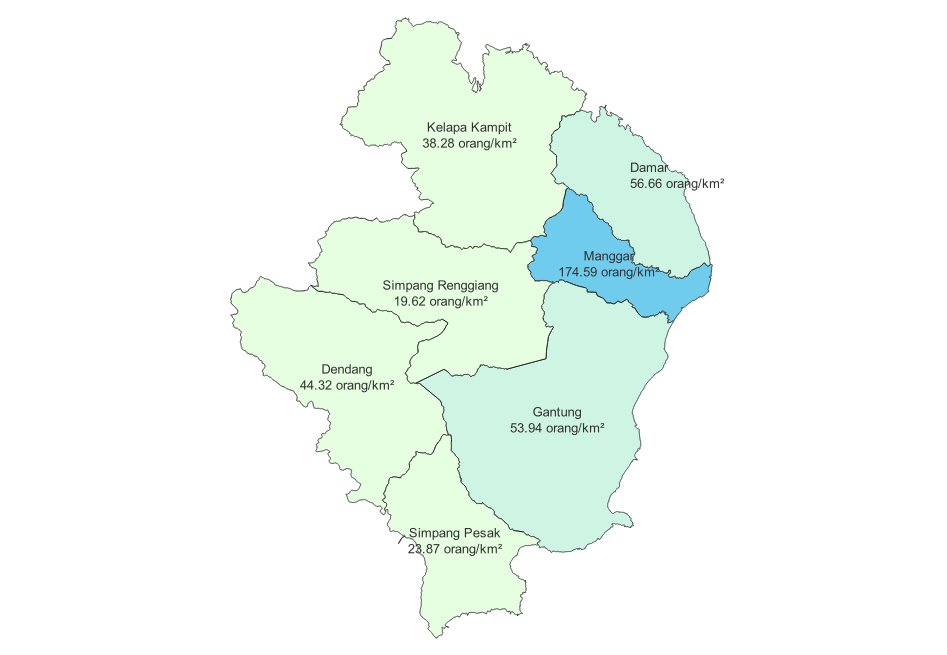
\includegraphics[width=0.85\textwidth]{bab_01/bab_01_01_kepadatanPenduduk}
	\caption{Kepadatan Penduduk di Kab. Belitung Timur Tahun \tP per Kecamatan}
	\label{fig:Kepadatan-Penduduk}
\end{figure}

Bila dikaitkan dengan pola distribusi secara spasial (\autoref{fig:Kepadatan-Penduduk}), maka terlihat
bahwa Kecamatan Manggar merupakan kecamatan dengan tingkat kepadatan
penduduk paling tinggi, sementara Kecamatan Simpang Renggiang merupakan
kecamatan dengan tingkat kepadatan penduduk paling rendah.

\subsection{Proporsi Penduduk Menurut Umur}
Proporsi penduduk menurut umur di Kabupaten Belitung Timur tahun
\tP dapat dilihat pada Piramida Penduduk Kab. Belitung Timur Tahun \tP (~\autoref{fig:Piramida-Penduduk-2022}).

\begin{figure}[!h]
    \centering{}
    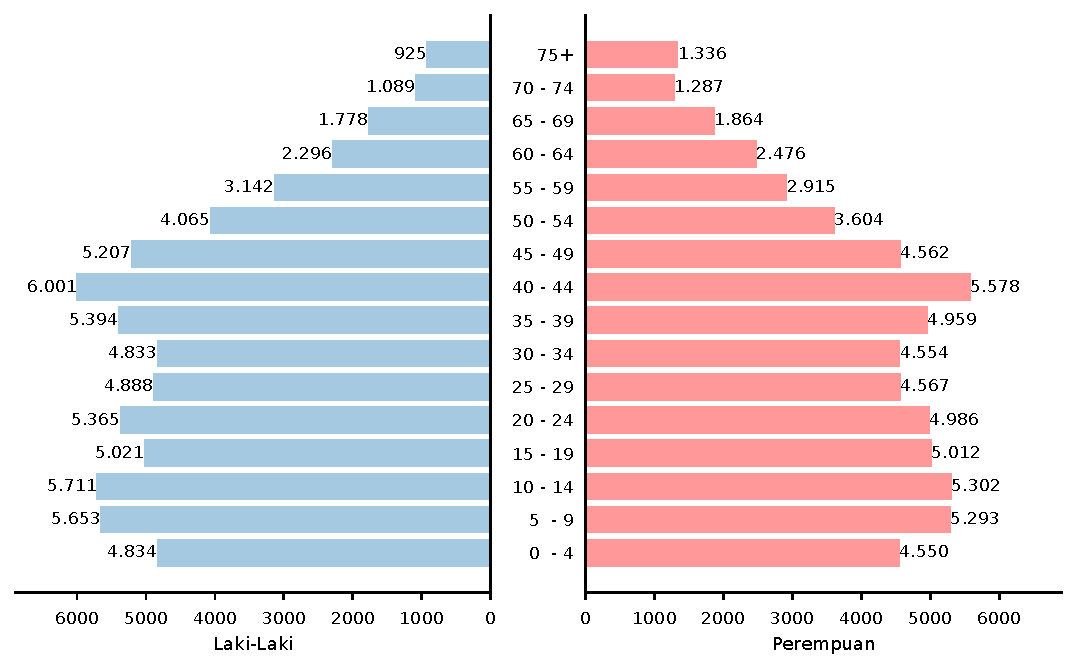
\includegraphics[width=\textwidth]{bab_01/bab_01_1_piramidaPenduduk}
%    \noindent\shadowimage[width=.9\textwidth]{bab_01/bab_01_1_piramidaPenduduk}
    \caption{Piramida Penduduk Kab. Belitung Timur Tahun \tP}
    \label{fig:Piramida-Penduduk-2022}
\end{figure}

Rasio beban tanggungan di kabupaten Belitung Timur adalah 44,31, yaitu setiap 100 orang penduduk usia produktif (umur 15 – 64 tahun) menanggung 44,31 orang penduduk usia non produktif (umur 0 – 14 tahun dan 65 – 75+ tahun).

\subsection{Proporsi Penduduk Menurut Jenis Kelamin}
Kabupaten Belitung Timur pada tahun \tP diproyeksi memiliki jumlah penduduk laki-laki sebesar 66.201 orang dan jumlah penduduk perempuan sebesar 62.847 orang, dengan total keseluruhan jumlah penduduk Kabupaten Belitung Timur yaitu 129.048 jiwa. Dengan demikian proporsi penduduk laki-laki adalah 51,30\% sedangkan proporsi penduduk perempuan adalah 48,70\% dengan rasio jenis kelamin sebesar 105,34 (\autoref{fig:Proporsi-Penduduk-Gender}).

\begin{figure}[!h]
    \centering{}
%    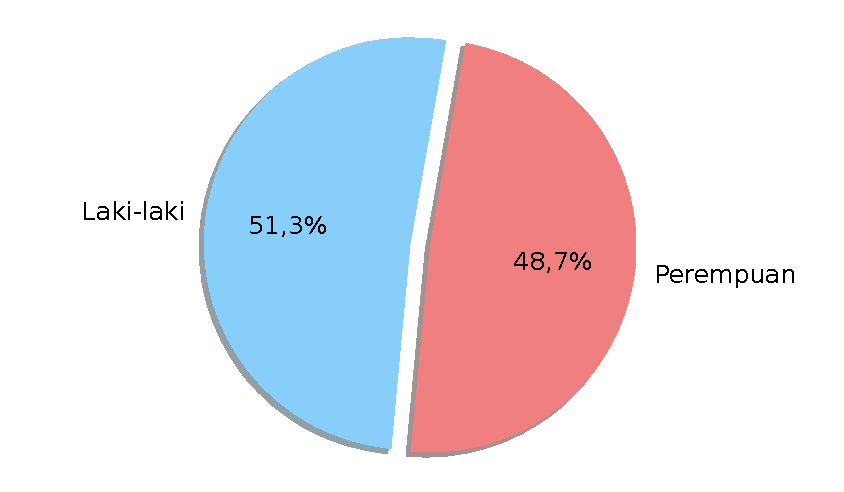
\includegraphics[width=0.7\textwidth]{bab_01/bab_01_2_distribusiGender}
%%    \noindent\shadowimage[width=.7\textwidth]{bab_01/bab_01_2_distribusiGender}
    \caption{Proporsi Penduduk Kab. Belitung Timur  Tahun \tP Menurut Jenis Kelamin}
    \label{fig:Proporsi-Penduduk-Gender}
\end{figure}

\section{KEADAAN PENDIDIKAN}
\todo{minta data BPS}
Komponen pengukuran tingkat pembangunan manusia suatu negara yang
cukup berpengaruh yaitu komponen pendidikan. Perubahan yang terjadi
secara terus menerus pada perilaku masyarakat disebabkan oleh semakin
meningkatnya tingkat pendidikan. Pendidikan juga merupakan salah satu
syarat mutlak pencapaian tujuan pembangunan manusia, dan merupakan
target pembangunan sekaligus sarana pembangunan nasional.

Salah satu capaian dalam bidang pendidikan yaitu kepemilikan ijazah
atau Surat Tanda Tamat Belajar (STTB), yang pada akhirnya akan menjadi
jalan untuk melanjutkan pendidikan ke jenjang pendidikan yang lebih
tinggi atau menjadi dasar untuk mencari pekerjaan yang sesuai. Selain
itu, ijazah/ STTB biasanya juga menjadi tolok ukur dalam pergaulan
atau hubungan sosial. Terkait dengan kualitas hidup manusia, ada kecenderungan semakin tinggi
ijazah/ STTB yang dimiliki maka pengetahuan pun semakin banyak dan
berakibat pada meningkatnya kualitas hidup terutama di bidang kesehatan
dan perumahan.

Pada tahun \tP diperkirakan terdapat 10,49\% penduduk Kabupaten Belitung Timur berusia di atas 15 tahun yang tidak memiliki ijazah SD/ sederajat. Sebanyak 32,26\% penduduk memiliki ijazah tertinggi berupa pendidikan dasar, yaitu telah menamatkan pendidikan SMA atau sederajat. Sebanyak 7,74\% penduduk telah menamatkan pendidikan tinggi (Diploma/ Sarjana) (\autoref{fig:Tingkat-Pendidikan}).

\begin{figure}[H]
    \centering
%    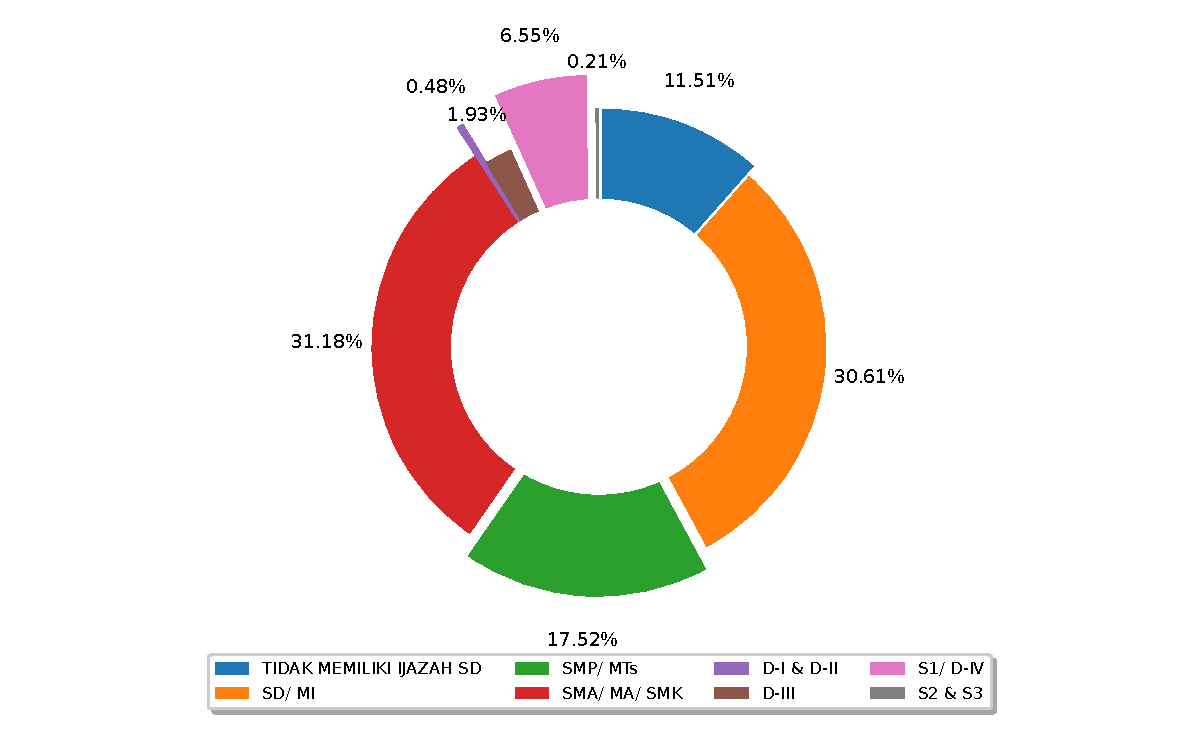
\includegraphics[width=0.9\textwidth]{bab_01/bab_01_03_distribusiPendidikan}
%    %\shadowimage[width=.7\textwidth]{bab_01/bab_01_03_distribusiPendidikan}
    \caption{Distribusi Penduduk Kab. Belitung Timur Tahun \tP Menurut Tingkat Pendidikan}
    \label{fig:Tingkat-Pendidikan}
\end{figure}

\clearpage
\chapter{SARANA PRASARANA KESEHATAN}
Pelayanan kesehatan kepada masyarakat harus didukung dengan sarana dan prasarana/ fasilitas yang memadai. Fasilitas pelayanan harus tersedia dan terdistribusi secara merata dalam jumlah dan jenis, serta berkualitas sesuai dengan kebutuhan masyarakat akan pelayanan kesehatan. 

\section{FASILITAS PELAYANAN KESEHATAN}
Undang-Undang Nomor 17 Tahun 2023 tentang Kesehatan menjelaskan bahwa fasilitas pelayanan kesehatan adalah suatu alat dan/atau tempat yang digunakan untuk menyelenggarakan upaya pelayanan kesehatan, baik promotif, preventif, kuratif, maupun rehabilitatif yang dilakukan oleh pemerintah, pemerintah daerah, dan/atau masyarakat. Penyelenggaraan Fasyankes diatur antara lain dalam Peraturan Menteri Kesehatan Republik Indonesia Nomor 75 Tahun 2014 Tentang Puskesmas serta Peraturan Menteri Kesehatan Republik Indonesia Nomor 56 Tahun 2014 Tentang Klasifikasi dan Perizinan Rumah Sakit.

\subsection{Rumah Sakit}
Rumah Sakit adalah Fasilitas Pelayanan Kesehatan yang menyelenggarakan Pelayanan Kesehatan perseorangan secara paripurna melalui Pelayanan Kesehatan promotif, preventif, kuratif, rehabilitatif, dan/ atau paliatif dengan menyediakan pelayanan rawat inap, rawat jalan, dan Gawat Darurat.\footnote{UU No 17 Tahun 2023, pasal 1}. Rumah Sakit menyelenggarakan fungsi\footnote{UU No 17 Tahun 2023, pasal 184}:
\begin{enumerate}
  \item Pelayanan Kesehatan perseorangan dalam bentuk spesialistik dan atau subspesialistik;
  \item Pelayanan Kesehatan dasar; dan
  \item Pendidikan dan penelitian di bidang kesehatan;
\end{enumerate}

Jumlah Rumah Sakit di Kabupaten Belitung Timur pada tahun \tP adalah sebanyak 1 (Satu) unit Rumah Sakit Umum, yaitu RSUD Muhammad Zein.

\subsection{Puskesmas}

Pusat Kesehatan Masyarakat (Puskesmas) adalah Fasilitas Pelayanan Kesehatan tingkat pertama yang menyelenggarakan dan mengoordinasikan
Pelayanan Kesehatan promotif, preventif, kuratif, rehabilitatif, dan atau paliatif dengan mengutamakan promotif dan preventif di wilayah kerjanya\footnote{UU No 17 Tahun 2023, pasal 1}. Puskesmas memiliki fungsi penyelenggaraan Pelayanan Kesehatan primer di wilayah kerjanya\footnote{UU No 17 Tahun 2023, pasal 180}. Puskesmas juga berperan mewujudkan wilayah kerja yang sehat dengan masyarakat yang:
\begin{enumerate}[label=\alph*]
	\item berperilaku hidup sehat;
	\item mudah mengakses Pelayanan Kesehatan bermutu;
	\item hidup dalam lingkungan sehat; dan
	\item memiliki derajat Kesehatan yang setinggi-tingginya, baik individu, keluarga, kelompok, maupun masyarakat.
\end{enumerate}

Jumlah Puskesmas menurut kecamatan di Kabupaten Belitung Timur tahun \tP adalah sebanyak 7 (enam) unit Puskesmas dengan rincian 4 (empat) unit Puskesmas Keperawatan yaitu Puskesmas Gantung, Puskesmas Simpang Pesak, Puskesmas Renggiang dan Puskesmas Kelapa Kampit, sedangkan 3 (dua) unit Puskesmas Non Keperawatan adalah Puskesmas Manggar, Puskesmas Mengkubang, dan Puskesmas Dendang.

\begin{figure}[H]
	\centering
%	maps better displayed in full width 
	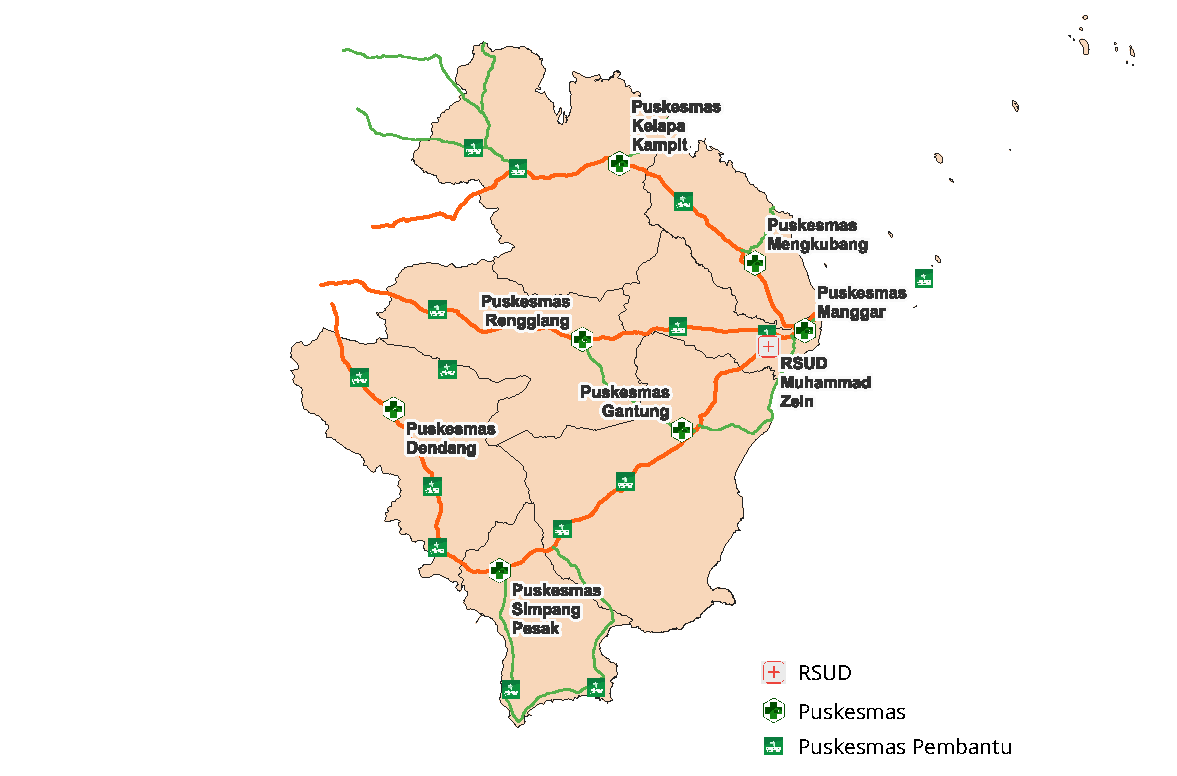
\includegraphics[width=\textwidth]{bab_02/bab_02_01_petaFaskes}	
	\caption{Lokasi Rumah Sakit, Puskesmas dan Puskesmas Pembantu di Kab. Belitung Timur}
	\label{fig:peta-puskesmas-rs}
\end{figure}

\subsection{Puskesmas Pembantu}

Puskesmas Pembantu merupakan jaringan pelayanan Puskesmas yang memberikan pelayanan kesehatan secara permanen di suatu lokasi dalam wilayah kerja Puskesmas\footnote{Permenkes No 75 Tahun 2014. pasal 40 ayat (2)}. Puskesmas  Pembantu merupakan bagian integral  Puskesmas, yang harus dibina secara berkala oleh Puskesmas.

Jumlah Puskesmas Pembantu di Kabupaten Belitung Timur pada tahun \tP adalah sebanyak 16 (Enam Belas) Pustu (\autoref{tab:Puskemas-dan-Pustu}).

\begin{table}[!ht]
\caption{Puskemas dan Jumlah Puskesmas Pembantu di Kab. Belitung Timur Tahun \tP}
\label{tab:Puskemas-dan-Pustu}
\centering{}%
\ra{1.3}

\begin{tabular}{lllr}
	\toprule
    No & Kecamatan & Puskesmas & Jumlah Puskesmas Pembantu\\
    \midrule
	1.                    & Manggar           & Manggar       & 3 \\
	\rowcolor{black!10}2. & Damar             & Mengkubang    & 1 \\
	3.                    & Gantung           & Gantung       & 3 \\
	\rowcolor{black!10}4. & Kelapa Kampit     & Kelapa Kampit & 2 \\
	5.                    & Simpang Renggiang & Renggiang     & 2 \\
	\rowcolor{black!10}6. & Simpang Pesak     & Simpang Pesak & 2 \\
	7.                    & Dendang           & Dendang       & 3 \\
    \midrule
    \multicolumn{2}{c}{Jumlah}                & 7             & 16\\
    \bottomrule
\end{tabular}
\end{table}

\section{AKSES DAN MUTU PELAYANAN KESEHATAN}
\todo{data dan grafik}
\subsection{Kunjungan Rawat Jalan dan Rawat Inap}
Kunjungan rawat jalan adalah kunjungan ke fasilitas pelayanan kesehatan tingkat pertama dan fasilitas pelayanan kesehatan rujukan tingkat lanjut milik pemerintah dan swasta untuk mendapatkan pelayanan kesehatan perseorangan yang meliputi observasi, diagnosa, pengobatan, rehabilitasi medik tanpa tinggal di ruang rawat inap untuk pertama kalinya dalam satu tahun tertentu. Kunjungan rawat jalan puskesmas termasuk kunjungan ke jaringan puskesmas, dalam gedung maupun luar gedung (puskesmas keliling, puskemas pembantu, bidan desa, pemeriksaan anak sekolah, dsb).
Kunjungan rawat inap adalah kunjungan ke fasilitas pelayanan kesehatan tingkat pertama dan fasilitas pelayanan kesehatan rujukan tingkat lanjut milik pemerintah dan swasta untuk mendapatkan pelayanan kesehatan perseorangan yang meliputi observasi, diagnosa, pengobatan, rehabilitasi medik, dan tinggal di ruang rawat inap untuk pertama kalinya dalam satu tahun tertentu.

Pada tahun \tP tercatat sebanyak 238.731 kunjungan di fasilitas layanan kesehatan di Kabupaten Belitung Timur. Sebanyak 157.915 kunjungan adalah ke fasilitas kesehatan milik pemerintah, sedangkan kunjungan ke fasilitas kesehatan milik swasta adalah sebanyak 80.816 kunjungan (\autoref{fig:Kunjungan-Faskes}).

Pada tahun \tP tercatat sebanyak 232.284 kali kunjungan rawat jalan dan 6.447 kunjungan rawat inap di fasilitas layanan kesehatan di Kabupaten Belitung Timur. Berdasarkan tingkat fasyankes, sebanyak 202.390 kunjungan adalah di Fasilitas Kesehatan Tingkat Pertama, sedangkan kunjungan di Fasilitas Kesehatan Tingkat Lanjutan adalah sebanyak 36.341 kunjungan (\autoref{fig:Kunjungan-Rawat}).

\begin{figure}[!htb]
    \centering{}
%    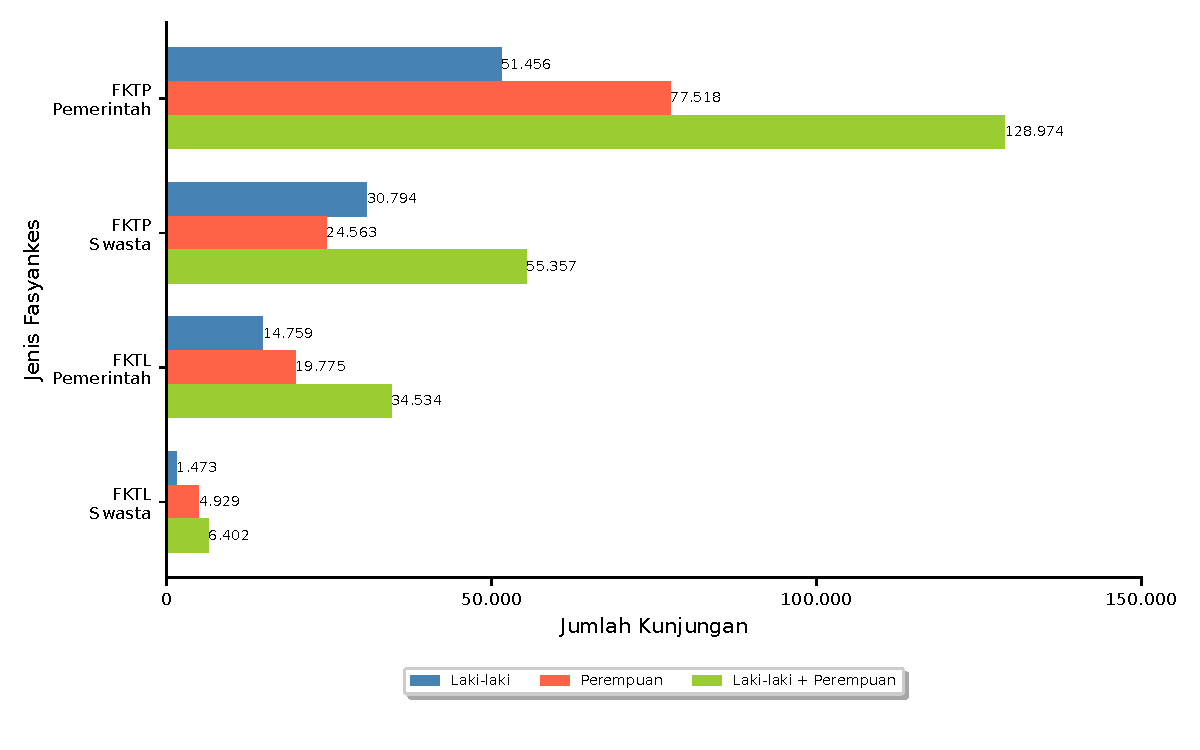
\includegraphics[width=0.9\textwidth]{bab_02/bab_02_1_kunjunganFaskes}
    \caption{Kunjungan Pasien Berdasarkan Jenis Faskes di Kab. Belitung Timur Tahun \tP}
    \label{fig:Kunjungan-Faskes}
\end{figure}

\begin{figure}[!htb]
    \centering{}
%    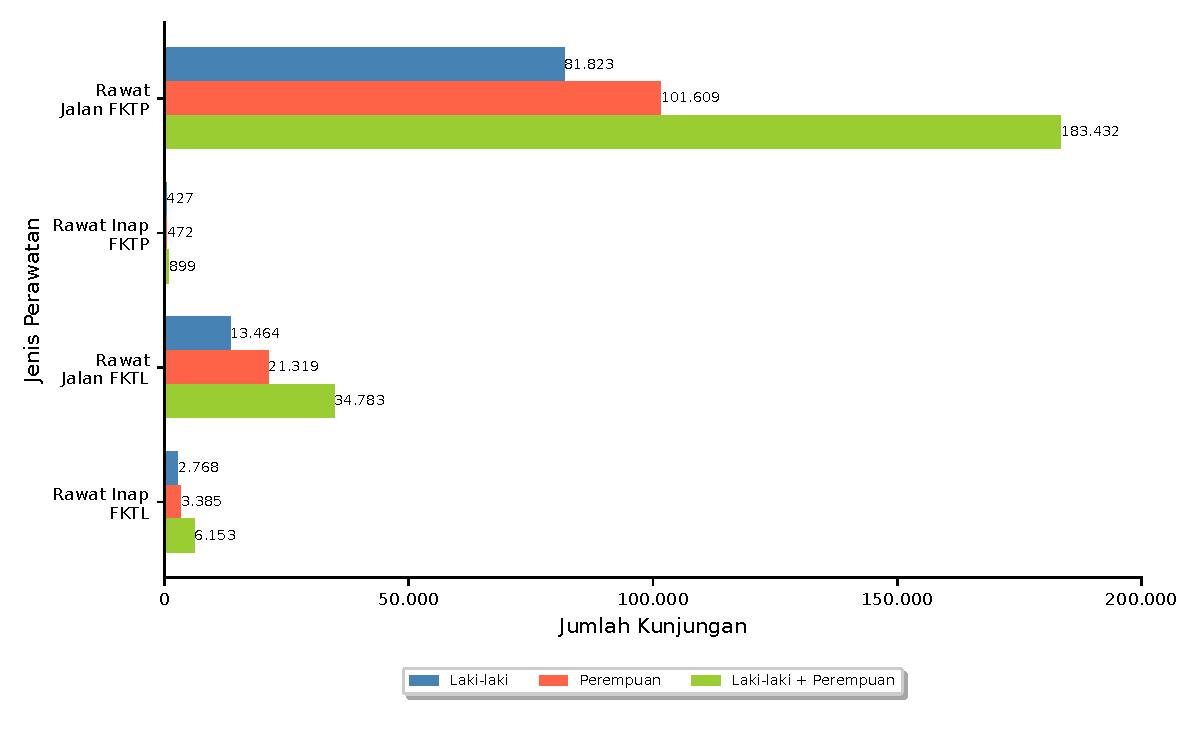
\includegraphics[width=0.9\textwidth]{bab_02/bab_02_2_rawat}
    \caption{Kunjungan Pasien Berdasarkan Jenis Perawatan di Kab. Belitung Timur Tahun \tP}
    \label{fig:Kunjungan-Rawat}
\end{figure}

\subsection{Kinerja Pelayanan Rumah Sakit}
Kinerja pelayanan rumah sakit dapat dinilai berdasarkan beberapa indikator, antara lain:
\begin{itemize}
 \item \emph{Gross Death Rate}(GDR), yaitu angka kematian umum untuk tiap-tiap 1.000 pasien keluar;
 \item \emph{Net Death Rate} (NDR), yaitu angka kematian ≥ 48 jam setelah dirawat untuk tiap-tiap 1.000 pasien keluar;
 \item \emph{Bed Occupancy Rate} (BOR), yaitu persentase pemakaian tempat tidur pada satu-satuan waktu tertentu;
 \item \emph{Bed Turn Over} (BTO), yaitu frekuensi pemakaian tempat tidur pada satu periode, berapa kali tempat tidur dipakai dalam satu satuan waktu;
 \item \emph{Turn Over Interval} (TOI), yaitu rata-rata hari tempat tidur tidak ditempati dari saat terisi ke saat terisi berikutnya; dan
 \item \emph{Average Length of Stay} (ALOS), yaitu rata-rata lama rawat (dalam satuan hari) seorang pasien.
\end{itemize}

Kinerja pelayanan rumah sakit di Kabupaten Belitung Timur pada tahun \tP dirangkum pada \autoref{tab:Kinerja-RS}.

\begin{table}[!ht]
\caption{Kinerja Pelayanan Rumah Sakit di Kab. Belitung Timur Tahun \tP}
\label{tab:Kinerja-RS}
\centering{}%
\ra{1.3}

\begin{tabular}{rlrr}
    \toprule
    No & Indikator                                          & Cakupan \tP       & Kondisi Ideal\\
    \midrule                                                
    1. & \emph{Gross Death Rate}                            & 66,27 per 1.000   & $\leq$ 45 per 1.000\\
    \rowcolor{black!10}2. & \emph{Net Death Rate}           & 30,80 per 1.000   & $\leq$ 25 per 1.000\\
    3. & \emph{Bed Occupancy Rate}                          & 47,02\%           & 60\% - 80\%\\
    \rowcolor{black!10}4. & \emph{Bed Turn Over}            & 46,18 kali        & 40 - 50 kali\\
    5. & \emph{Turn Over Interval}                          & 4,19 hari         & 1 - 3 hari\\
    \rowcolor{black!10}6. & \emph{Average Length of Stay}   & 3,76 hari         & 6 - 9 hari\\
    \bottomrule
\end{tabular}
\end{table}

\subsection{Ketersediaan Obat Esensial dan Vaksin IDL}
\subsubsection{Ketersediaan obat esensial}
Obat esensial adalah 40 item obat indikator yang merupakan obat pendukung Program Kesehatan Ibu dan Anak, Program Gizi, Program TB Paru, Program Malaria, serta obat pelayanan kesehatan dasar esensial dan terdapat di dalam Formularium Nasional.

Persentase Puskesmas dengan ketersediaan obat esensial adalah persentase Puskesmas yang memiliki ketersediaan minimal 80\% dari 40 item obat indikator pada saat dilakukan pemantauan terhadap
seluruh puskesmas yang melaporkan data. Laporan yang disampaikan yaitu laporan pada bulan November atau laporan bulan terakhir pada tahun pelaporan.

Pada tahun \tP terdapat 100\% Puskesmas yang memenuhi ketersediaan obat esensial di Kabupaten Belitung Timur.

\subsubsection{Ketersediaan vaksin IDL}
Vaksin Imunisasi Dasar Lengkap (IDL) terdiri dari Vaksin Hepatitis B, Vaksin BCG, Vaksin DPT-HB-HIB, Vaksin Polio dan Vaksin Campak/Campak Rubella.

Ketersediaan vaksin IDL adalah persentase Puskesmas yang memiliki vaksin IDL pada saat dilakukan pemantauan terhadap seluruh puskesmas yang melaporkan data. Laporan yang dimasukkan yaitu laporan pada bulan November atau laporan bulan terakhir pada tahun pelaporan.

Pada tahun \tP terdapat 100\% Puskesmas yang memenuhi ketersediaan vaksin IDL di Kabupaten Belitung Timur.


\section[UKBM]{UPAYA KESEHATAN BERSUMBERDAYA MASYARAKAT (UKBM)}% for title and page
\sectionmark{UKBM} %for header
\subsection{Posyandu}
Posyandu adalah salah satu bentuk Upaya Kesehatan Bersumberdaya Masyarakat (UKBM) yang dikelola dan diselenggarakan dari, oleh, untuk, dan bersama masyarakat guna memberdayakan masyarakat dan memberikan kemudahan kepada masyarakat dalam memperoleh pelayanan kesehatan dasar untuk mempercepat penurunan angka kematian ibu, bayi, dan balita. Posyandu melayani kegiatan berupa penimbangan bayi dan balita, pemberian imunisasi, konsultasi kesehatan dan Pemberian Makanan Tambahan (PMT).

Jumlah Posyandu di Kabupaten Belitung Timur tahun \tP adalah sebanyak 133 posyandu aktif dari total 133 unit posyandu (\autoref{fig:Posyandu-Aktif}).

\begin{figure}[H]
	\centering{}
%	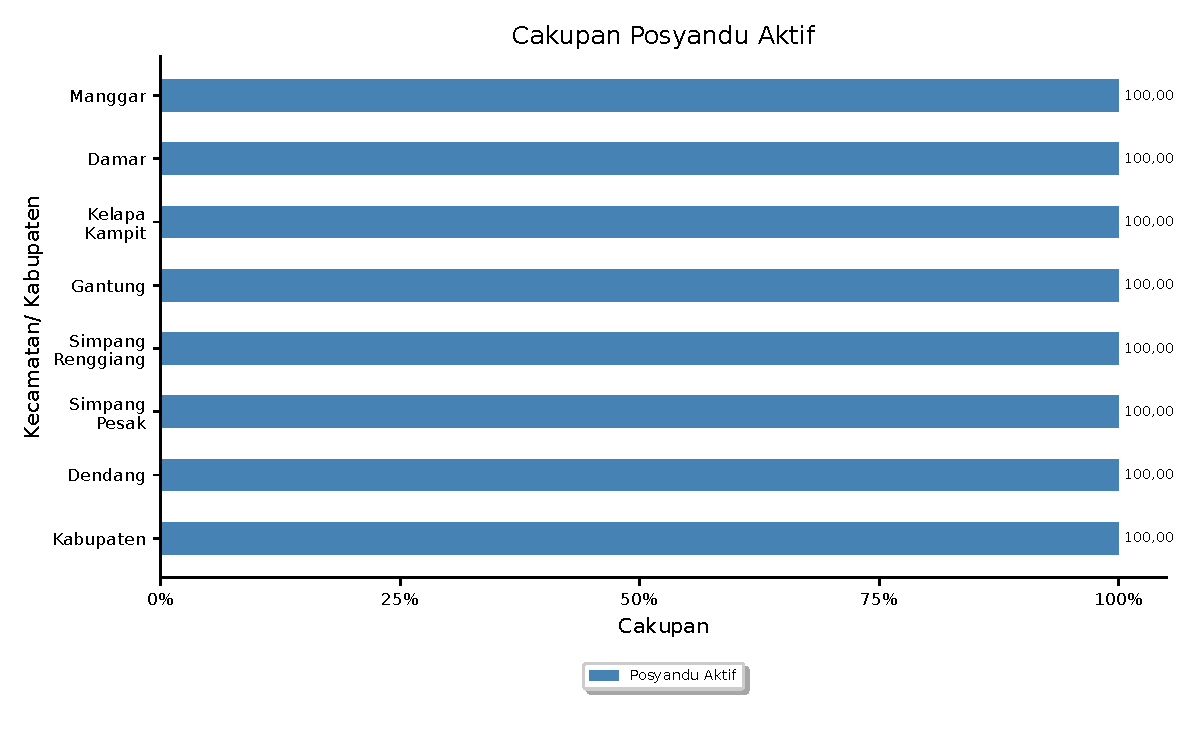
\includegraphics[width=0.9\textwidth]{bab_02/bab_02_3_posyandu}
	\caption{Persentase Posyandu Aktif di Kab. Belitung Timur Tahun \tP}
	\label{fig:Posyandu-Aktif}
\end{figure}

\subsection{Posbindu PTM}
Posbindu PTM adalah suatu upaya kesehatan berbasis bersumberdaya masyarakat (UKBM) dalam pencegahan dan pengendalian Penyakit Tidak Menular (PTM) melalui kegiatan skrining kesehatan/ deteksi dini faktor risiko PTM, intervensi/ modifikasi faktor risiko PTM serta monitoring dan tindak lanjut faktor risiko PTM bersumber daya masyarakat secara rutin dan berkesinambungan.

Jumlah Posbindu PTM di Kabupaten Belitung Timur tahun \tP adalah sebanyak 62 Posbindu PTM. %(\autoref{tab:Posyandu-Posbindu-di-Kab}).

\clearpage
\chapter{SUMBER DAYA MANUSIA KESEHATAN}
Pelayanan kesehatan kepada masyarakat harus didukung dengan tenaga kesehatan, yang berkompetensi. Untuk menjalankan fungsi pengembangan, Dinas Kesehatan Kabupaten Belitung Timur sebagai fasilitator dan koordinator dalam pendidikan dan pelatihan sumber daya kesehatan dengan kebijakan bahwa semua bentuk pelatihan yang dilaksanakan oleh Dinas Kesehatan Kabupaten Belitung Timur dalam meningkatkan kinerja tenaga kesehatan. Sedangkan di setiap UPTD Puskesmas dan Subbagian/ Bidang berkoordinasi dalam perencanaan dan diklat. Hal ini untuk meningkatkan efesiensi dan efektifitas diklat dan menghindari \textit{overlapping} jenis dan kuantitas diklat.

Pelaksanaan program sumber daya manusia kesehatan bertujuan untuk meningkatkan jumlah, jenis, mutu dan penyebaran tenaga kesehatan serta pemberdayaan profesi kesehatan, yang sesuai dengan kebutuhan. Peningkatan keterampilan dan profesionalisme tenaga kesehatan yaitu dengan pendidikan dan pelatihan tenaga kesehatan, dan menyusun standar kompetensi dan regulasi profesi.

Kebutuhan tenaga kesehatan ditentukan oleh pemenuhan rasio tenaga kesehatan berdasarkan jumlah penduduk pada tingkat kabupaten serta pemenuhan standar ketenagaan minimal pada tingkat fasilitas pelayanan kesehatan (Puskesmas dan Rumah Sakit). Standar rasio tenaga kesehatan berdasarkan jumlah penduduk diatur dalam Keputusan Menteri Koordinator Bidang Kesejahteraan Rakyat Republik Indonesia Nomor 54 Tahun 2013 Tentang Rencana Pengembangan Tenaga Kesehatan Tahun 2011 – 2025. Sedangkan standar ketenagaan minimal pada tingkat fasilitas pelayanan kesehatan
diatur dalam Peraturan Menteri Kesehatan Republik Indonesia Nomor 75 Tahun 2014 Tentang Puskesmas serta Peraturan Menteri Kesehatan Republik Indonesia Nomor 56 Tahun 2014 Tentang Klasifikasi dan Perizinan Rumah Sakit.

Dalam memenuhi SDM kesehatan yang belum memenuhi standar rasio kesehatan penduduk dilakukan pengadaan, penetapan dan penyebaran tenaga kesehatan. Penambahan dan penetapan SDM kesehatan dilakukan kerjasama dengan pihak-pihak yang terkait, antara lain Departemen Kesehatan RI, Pemerintah Kabupaten, Pemerintah Provinsi. Program beasiswa dilakukan terus menerus dalam upaya peningkatan SDM Kesehatan ini. Sumber pembiayaan dari APBN, APBD Tk.I, maupun APBD Tk. II, setiap tahunnya ditargetkan untuk tugas belajar (Tubel) dengan pembagian yang merata di setiap Pusat Kesehatan yang ada di setiap kecamatan.

\section{TENAGA MEDIS}
Undang-undang Nomor 17 Tahun 2023 tentang Kesehatan mengatur bahwa yang termasuk dalam kelompok tenaga medis adalah dokter, dokter gigi, dokter spesialis, dan dokter gigi spesialis.
Dokter dan dokter gigi adalah dokter, dokter spesialis, dokter gigi, dan dokter gigi spesialis lulusan pendidikan kedokteran atau kedokteran gigi baik di dalam maupun di luar negeri yang diakui oleh Pemerintah Republik Indonesia sesuai dengan peraturan perundang-undangan.

Jumlah Dokter Umum di Kabupaten Belitung Timur pada tahun \tP adalah sebanyak 50 (Lima Puluh) orang dengan rasio 38,75 per 100.000 penduduk.
Dokter Spesialis di Kabupaten Belitung Timur tahun \tP berjumlah 17 (Tujuh Belas) orang dengan rasio 13,17 per 100.000 penduduk.
Dokter Gigi (termasuk Dokter Spesialis Gigi) berjumlah 9 (Sembilan) orang dengan rasio 6,97 per 100.000 penduduk.

\section{TENAGA KESEHATAN}
\subsection{Tenaga Keperawatan dan Kebidanan}
Perawat adalah seseorang yang telah lulus pendidikan tinggi keperawatan, baik di dalam maupun di luar negeri yang diakui oleh Pemerintah sesuai dengan ketentuan peraturan perundang-undangan.
Bidan adalah seorang perempuan yang lulus dari pendidikan bidan yang telah teregistrasi sesuai ketentuan peraturan perundang-undangan .

Jumlah tenaga kesehatan Perawat di Kabupaten Belitung Timur tahun \tP sebanyak 361 (Tiga Ratus Enam Puluh Satu) orang dengan rasio 279,74 per 100.000 penduduk.

Jumlah tenaga kesehatan Bidan di Kabupaten Belitung Timur tahun \tP adalah sebanyak 157 (Seratus Lima Puluh Tujuh) orang dengan rasio 121,66 per 100.000 penduduk.

\begin{table}[H]
\caption{Rasio Tenaga Kesehatan di Kab. Belitung Timur tahun \tP}
\label{tab:Rasio-Tenaga-Kesehatan}
\centering{}%
\ra{1.3}
\renewcommand*{\arraystretch}{1.3}

\begin{tabular}{rY{0.3\textwidth}rrr}
\toprule
\multicolumn{1}{c}{No} & \makecell[l]{Jenis\\Tenaga Kesehatan} & Jumlah & \makecell[r]{Rasio Tahun\\\tP (per 100.000\\penduduk)}
& \makecell[r]{Target Rasio Tahun\\\tP\footnotemark[1] (per 100.000\\ penduduk)}\\
\midrule
    1                     & Dokter Spesialis                         &  18 &  13,17 &  11 \\
    \rowcolor{black!10}2  & Dokter Umum                              &  62 &  38,75 &  45 \\
                       3  & Dokter Gigi                              &   9 &   6,97 &  13 \\
    \rowcolor{black!10}4  & Perawat                                  & 370 & 279,74 & 180 \\
                       5  & Bidan                                    & 179 & 121,66 & 120 \\
    \rowcolor{black!10}6  & Apoteker                                 &  15 &  11,62 &  12 \\
                       7  & Tenaga Teknis Kefarmasian                &  26 &  16,27 &  24 \\
    \rowcolor{black!10}8  & Tenaga Kesehatan Masyarakat              &  19 &  14,72 &  15 \\
                       9  & Tenaga Kesehatan Lingkungan              &  13 &   7,75 &  18 \\
    \rowcolor{black!10}10 & Tenaga Gizi                              &  22 &  17,82 &  14 \\
                       11 & Tenaga Ahli Teknologi Laboratorium Medik &  27 &  20,92 & N/A \\
    \rowcolor{black!10}12 & Tenaga Teknik Biomedika Lainnya          &  10 &   8,52 & N/A \\
                       13 & Tenaga Keterapian Fisik                  &   7 &   5,42 &   5 \\
    \rowcolor{black!10}14 & Tenaga Keteknisian Medis                 &  34 &  26,43 &  16\\
\bottomrule
\end{tabular}
\end{table}
\footnotetext[1]{Target Nasional RPTK Tahun 2011-2025 (Kepmenko Kesra No.54 Tahun 2013)}

\subsection{Tenaga Kesehatan Masyarakat, Kesehatan Lingkungan dan Tenaga Gizi}
Tenaga kesehatan masyarakat adalah tenaga kesehatan yang telah memenuhi kualifikasi bidang kesehatan masyarakat
yang terdiri dari epidemiolog kesehatan, tenaga promosi kesehatan dan ilmu perilaku, pembimbing kesehatan kerja,
tenaga administrasi dan kebijakan kesehatan, tenaga biostatistik dan kependudukan, serta tenaga kesehatan reproduksi
dan keluarga sesuai dengan peraturan perundang-undangan yang berlaku.
Tenaga kesehatan lingkungan adalah tenaga kesehatan yang telah memenuhi kualifikasi bidang kesehatan lingkungan yang terdiri dari sanitasi lingkungan,
entomolog kesehatan, mikrobiolog kesehatan sesuai dengan peraturan perundang-undangan yang berlaku.
Tenaga gizi adalah tenaga kesehatan yang telah memenuhi kualifikasi bidang gizi yang terdiri dari nutrisionis dan dietisien
sesuai dengan peraturan perundang-undangan yang berlaku.

Jumlah tenaga Kesehatan Masyarakat berjumlah 19 (Sembilan Belas) orang dengan rasio 14,72 per 100.000 penduduk, tenaga Kesehatan Lingkungan sebanyak 10 (Sepuluh) orang dengan rasio 7,75 per 100.000 penduduk, dan tenaga Gizi berjumlah 23 (Dua Puluh Tiga) orang dengan rasio 17,82 per 100.000 penduduk.

\subsection{Tenaga Teknik Biomedika, Keterapian Fisik dan Keteknisan Medik}
Tenaga ahli teknologi laboratorium medik adalah setiap orang yang telah lulus pendidikan teknologi laboratorium medik atau analis
kesehatan atau analis medis dan memiliki kompetensi melakukan analisis terhadap cairan dan jaringan tubuh manusia untuk
menghasilkan informasi tentang kesehatan perseorangan dan masyarakat sesuai dengan ketentuan peraturan perundang-undangan.
Tenaga teknik biomedika lainnya adalah tenaga kesehatan yang telah memenuhi kualifikasi bidang teknik biomedika yang terdiri dari radiografer, elektromedis, fisikawan medik, radioterapis, dan ortotik prostetik.

Tenaga keterapian fisik adalah tenaga kesehatan yang telah memenuhi kualifikasi bidang keterapian fisik yang terdiri
dari fisioterapis, okupasi terapis, terapis wicara, dan akupunktur sesuai dengan peraturan perundang-undangan yang
berlaku.
Tenaga keteknisian medis adalah tenaga kesehatan yang telah memenuhi kualifikasi bidang keteknisian medis yang
terdiri dari perekam medis dan informasi kesehatan, teknik kardiovaskuler, teknisi pelayanan darah, refraksionis
optisien/ optometris, teknisi gigi, penata anestesi (perawat anastesi), terapis gigi dan mulut (perawat gigi), dan audiologis.

Jumlah tenaga kesehatan Ahli Teknologi Laboratorium Medik di Kabupaten Belitung Timur tahun
\tP adalah sebanyak 27 (Dua Puluh Tujuh) orang dengan rasio 20,92 per 100.000 penduduk.
Jumlah tenaga kesehatan Tenaga Teknik Biomedika Lainnya adalah sebanyak 11 (Sepuluh) orang dengan rasio 8,52 per 100.000 penduduk.

Jumlah tenaga Keterapian Fisik adalah sebanyak 7 (Tujuh) orang dengan rasio 5,42 per 100.000 penduduk. Sedangkan jumlah tenaga Keteknisian Medis adalah 37 (Tiga Puluh Tujuh) orang dengan rasio 28,67 per 100.000 penduduk.


\subsection{Tenaga Kefarmasian}
Tenaga kefarmasian adalah tenaga kesehatan yang telah memenuhi kualifikasi bidang kefarmasian yang terdiri dari apoteker dan tenaga teknis kefarmasian sesuai dengan peraturan perundang-undangan yang berlaku.
Apoteker adalah Sarjana Farmasi yang telah lulus sebagai Apoteker dan telah mengucapkan sumpah jabatan Apoteker.
Tenaga Teknis Kefarmasian adalah tenaga yang membantu Apoteker dalam menjalankan pekerjaan kefarmasian, yang terdiri atas Sarjana Farmasi, Ahli Madya Farmasi, Analis Farmasi dan Tenaga Menengah Farmasi/ Asisten Apoteker.

Jumlah Apoteker di Kabupaten Belitung Timur di tahun \tP adalah sebanyak 15 (Lima Belas) orang dengan rasio 11,62 per 100.000 penduduk. Sedangkan jumlah tenaga teknis kefarmasian adalah 21 (Dua Puluh Satu) orang dengan rasio 16,27 per 100.000 penduduk.

\vspace{2ex}

Rincian lebih lengkap mengenai jumlah tenaga kesehatan di Kabupaten Belitung Timur pada tahun \tP dapat dilihat pada Lampiran Tabel Profil (tabel 13-17).
 %done
\clearpage
% \chapter{PEMBIAYAAN KESEHATAN}
Pembiayaan kesehatan bertujuan untuk penyediaan pembiayaan kesehatan yang berkesinambungan dengan jumlah yang mencukupi, teralokasi secara adil, dan termanfaatkan. Pembiayaan kesehatan merupakan besarnya dana yang harus disediakan untuk menyelenggarakan dan atau memanfaatkan berbagai upaya kesehatan yang diperlukan oleh perorangan, keluarga, kelompok, dan masyarakarat.

Secara umum, sumber biaya kesehatan dapat dibedakan menjadi pembiayaan yang bersumber dari anggaran pemerintah dan pembiayaan yang bersumber dari masyarakat.

\section[PEMBIAYAAN OLEH MASYARAKAT]{PEMBIAYAAN KESEHATAN OLEH MASYARAKAT}
Pada saat ini berkembang berbagai upaya pembiayaan pelayanan kesehatan praupaya, antara lain Badan Penyelenggara Jaminanan Sosial Kesehatan (BKPJS Kesehatan) dan berbagai jasa asuransi kesehatan swasta. BPJS Kesehatan adalah Badan Hukum Publik yang bertanggung jawab langsung kepada Presiden dan memiliki tugas untuk menyelenggarakan Jaminan Kesehatan Nasional bagi seluruh rakyat Indonesia. Keanggotaan BPJS bersifat wajib bagi setiap warga negara Indonesia dan warga asing yang sudah bekerja di Indonesia selama minimal enam bulan. Setiap peserta BPJS akan ditarik iuran yang besarnya ditentukan kemudian, sesuai dengan tingkatan manfaat yang diinginkan.

Sejak tahun 2014, penyelenggaraan pelayanan kesehatan bagi masyarakat miskin meliputi pelayanan kesehatan dasar di Puskesmas dan jaringannya, serta upaya kesehatan rujukan di Rumah Sakit telah dialihkan ke pengelolaan oleh BPJS Kesehatan. Bagi warga miskin, iuran BPJS ditanggung pemerintah melalui program Penerima Bantuan Iuran (PBI) yang dananya bersumber dari APBN maupun APBD Provinsi/ Kabupaten/ Kota.

Cakupan jaminan kesehatan melalui BPJS Kesehatan di Kabupaten Belitung Timur pada tahun \tP adalah sebesar 98,92\% dari jumlah penduduk, di mana 63,46\%  dari jumlah penduduk adalah Penerima Bantuan Iuran (PBI) bersumber APBD dan APBN (\autoref{fig:Cakupan-BPJS}).
%Diperkirakan terdapat 5.075 penduduk dari total 125.598 penduduk yang masih belum mendapat perlindungan jaminan kesehatan (\autoref{fig:Cakupan-Jamkes}).

\begin{figure}[H]
    \centering{}
    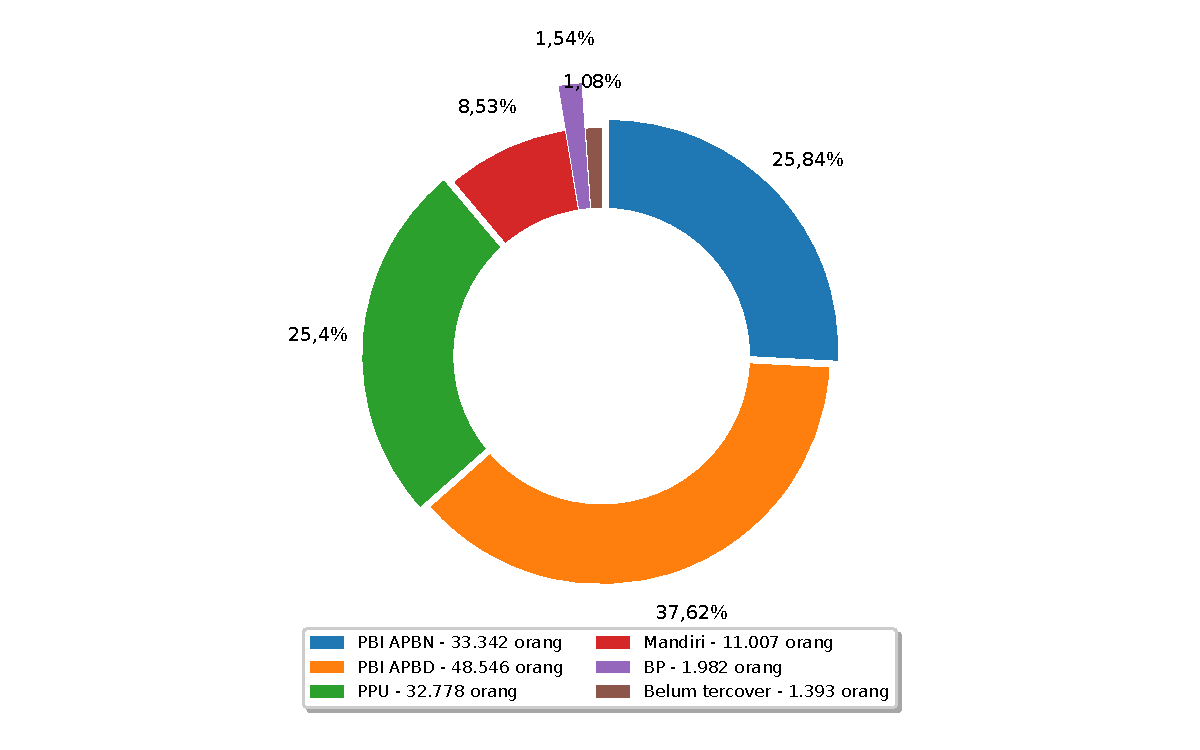
\includegraphics[width=0.9\textwidth]{bab_04/bab_04_01_jaminanKesehatan_a}
    \caption{Cakupan BPJS Kesehatan Kab. Belitung Timur Tahun \tP}
    \label{fig:Cakupan-BPJS}
\end{figure}

\begin{figure}[H]
    \centering{}
    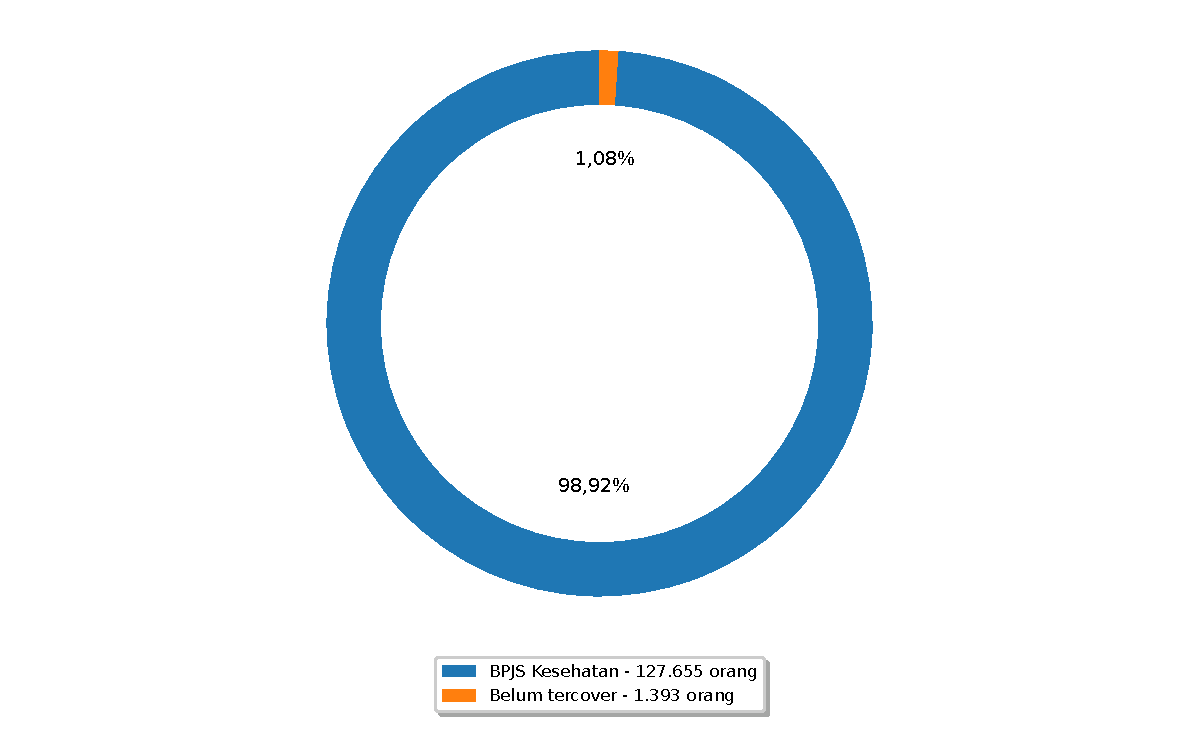
\includegraphics[width=0.9\textwidth]{bab_04/bab_04_01_jaminanKesehatan_b}
    \caption{Cakupan Jaminan Kesehatan Kab. Belitung Timur Tahun \tP}
    \label{fig:Cakupan-Jamkes}
\end{figure}

\section[PEMBIAYAAN OLEH PEMERINTAH]{PEMBIAYAAN KESEHATAN OLEH PEMERINTAH}
\subsection{Pembiayaan Melalui Anggaran Pendapatan dan Belanja Daerah}
Alokasi Anggaran Kesehatan di Kabupaten Belitung Timur pada tahun \tP melalui APBD Kabupaten Belitung Timur Tahun \tP (mencakup anggaran Dinas Kesehatan, UPTD Kesehatan dan RSUD Belitung Timur) adalah sebesar Rp XXXX. Nilai anggaran ini terdiri dari sumber APD murni sebesar Rp XXXX, Dana Alokasi Khusus (DAK) berupa DAK Fisik sebesar Rp XXX dan DAK Non-Fisik sebesar Rp XXXX. Selain itu terdapat anggaran belanja bersumber APBN berupa dana kapitasi sebesar Rp XXXX.

Porsi alokasi anggaran kesehatan adalah sebesar XXXX\% dari jumlah belanja APBD Kabupaten Belitung Timur Tahun \tP sebesar Rp XXX. Sedangkan alokasi anggaran kesehatan per kapita adalah sebesar Rp 2.294.066,00 /kapita.

\begin{figure}[htb]
    \centering{}
%    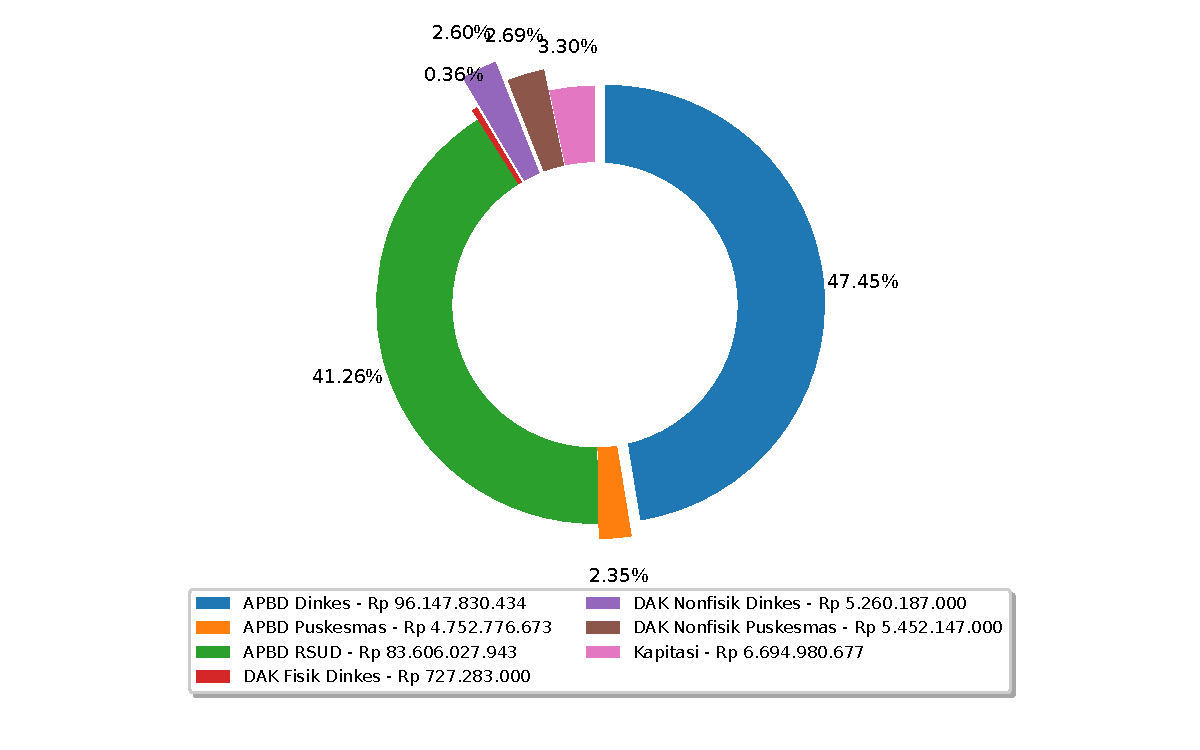
\includegraphics[width=0.9\textwidth]{bab_04/bab_04_03_anggaranKesehatan}
    \caption{Persentase Anggaran Kesehatan Kab. Belitung Timur Tahun \tP}
    \label{fig:Anggaran-Kesehatan}
\end{figure}

\subsection{Pembiayaan Jaminan Kesehatan Masyarakat Pada Anggaran Dinas Kesehatan}
Pembiayaan jaminan kesehatan masyarakat berupa iuran dan bantuan iuran jaminan kesehatan bagi peserta PBPU dan BP kelas 3 dianggarkan pada anggaran Dinas Kesehatan, Pengendalian Penduduk dan Keluarga Berencana Kabupaten Belitung Timur melalui Program Pemenuhan Upaya Kesehatan Perorangan Dan Upaya Kesehatan Masyarakat, Kegiatan Penyediaan Layanan Kesehatan untuk UKM dan UKP Rujukan Tingkat Daerah Kabupaten/Kota, Subkegiatan Pengelolaan Jaminan Kesehatan Masyarakat. Pada tahun \tP belanja iuran jaminan tersebut dianggarkan sebesar Rp 18.799.200.000 atau sebesar 18,41\% dari anggaran Dinas Kesehatan Kabupaten Belitung Timur.

\begin{figure}[htb]
	\centering{}
	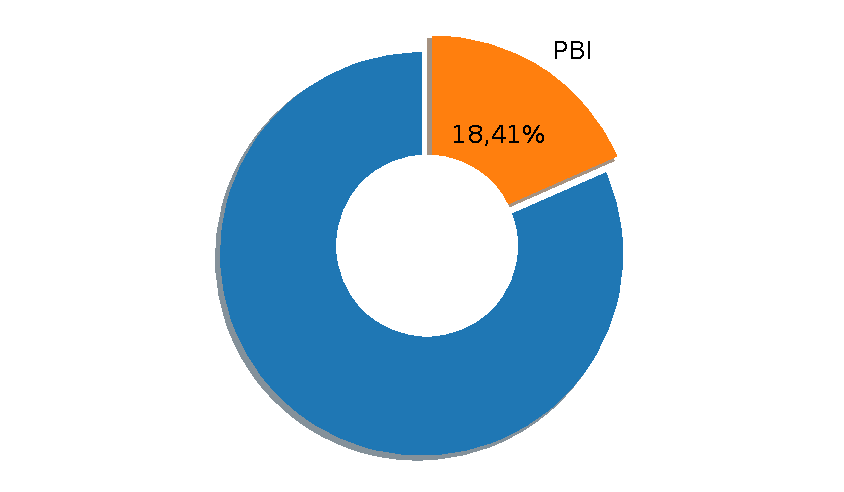
\includegraphics[width=0.9\textwidth]{bab_04/bab_04_04_proporsiPBI}
	\caption{Proporsi PBI terhadap Anggaran DKPPKB Kab. Belitung Timur Tahun \tP}
	\label{fig:Proporsi-PBI}
\end{figure}
 %done
% \clearpage
\chapter{KESEHATAN KELUARGA}
Pembangunan keluarga dilakukan dalam upaya untuk mewujudkan keluarga berkualitas yang hidup dalam lingkungan yang sehat. Selain lingkungan yang sehat, kondisi kesehatan dari tiap anggota keluarga sendiri juga merupakan salah satu syarat dari keluarga yang berkualitas.
Keluarga berperan terhadap optimalisasi pertumbuhan, perkembangan, dan produktivitas seluruh anggotanya melalui pemenuhan kebutuhan gizi dan menjamin kesehatan anggota keluarga. 

Di dalam komponen keluarga, ibu dan anak merupakan kelompok rentan terhadap keadaan keluarga dan sekitarnya secara umum.
Hal ini terkait dengan fase kehamilan, persalinan dan nifas pada ibu dan fase tumbuh kembang pada anak.
Oleh karena itu ibu dan anak merupakan anggota keluarga yang perlu mendapatkan prioritas dalam penyelenggaraan upaya kesehatan.

\section{KESEHATAN IBU}
Seorang ibu mempunyai peranan yang sangat penting dalam pertumbuhan anak dan bayi.
Hal ini terkait dengan fase kehamilan, persalinan dan nifas pada ibu dan fase tumbuh kembang pada anak.
Gangguan kesehatan yang dialami pada seorang ibu dapat mempengaruhi kesehatan janin dalam kandungan hingga kelahiran dan masa pertumbuhan bayi dan anaknya.

\subsection{Angka Kematian Ibu (AKI)}
Kematian ibu adalah kematian yang terjadi pada seorang ibu yang terjadi karena peristiwa kehamilan, persalinan, dan masa nifas (dalam kurun waktu 42 hari sejak terminasi kehamilan) tanpa memandang lamanya kehamilan, yakni kematian yang disebabkan karena kehamilannya atau penanganannya, tetapi bukan karena sebab-sebab lain seperti kecelakaan dan terjatuh.
Angka Kematian Ibu (AKI) menggambarkan status gizi dan tingkat pelayanan kesehatan terhadap ibu hamil, ibu melahirkan dan ibu masa nifas.

Jumlah Kematian Ibu di Kabupaten Belitung Timur pada tahun \tP adalah 3 orang, dengan Angka Kematian Ibu (AKI) 157,48 per 100.000 kelahiran hidup (\autoref{fig:Jumlah-Kematian-Ibu}). 
%Angka ini meningkat dari AKI tahun 2020 sebesar 189,84 per 100.000 kelahiran hidup(\autoref{fig:AKI-2017-2021}).

\begin{figure}[H]
    \centering{}
    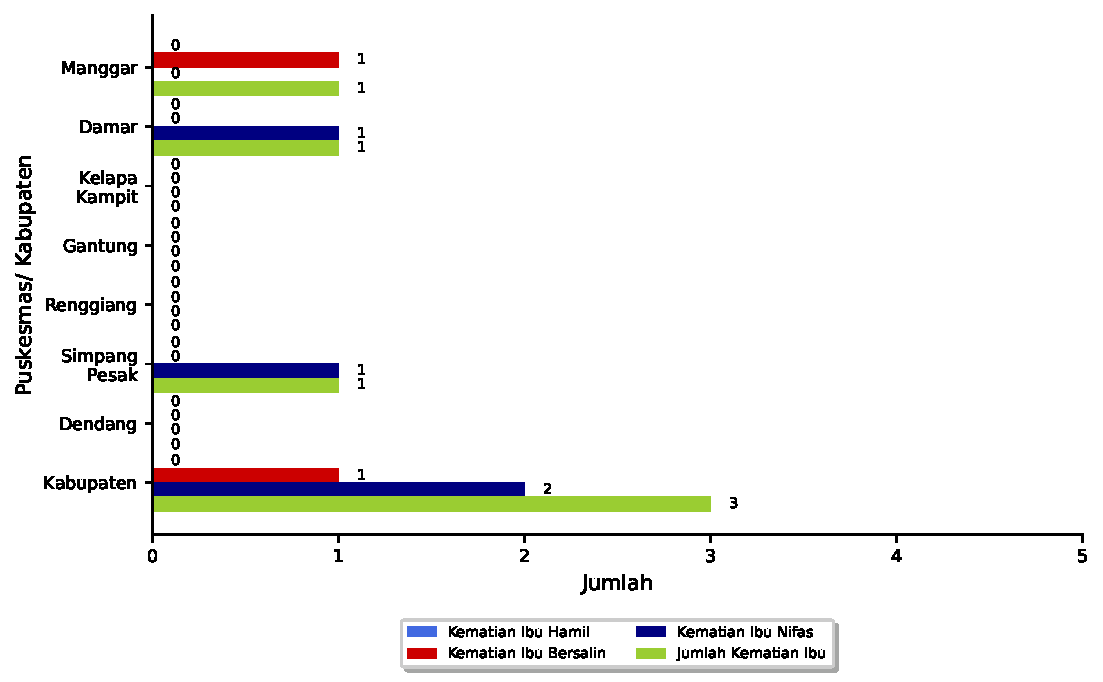
\includegraphics[width=0.9\textwidth]{bab_05/bab_05_01_kematianIbu}
%    \caption{Jumlah Kematian Ibu di Kab. Belitung Timur Tahun \tP per Puskesmas (hal. ~\pageref{C_21-Jumlah-Kematian-Ibu})}
    \caption{Jumlah Kematian Ibu di Kab. Belitung Timur Tahun \tP per Puskesmas}
    \label{fig:Jumlah-Kematian-Ibu}
\end{figure}

\begin{figure}[H]
    \centering{}
    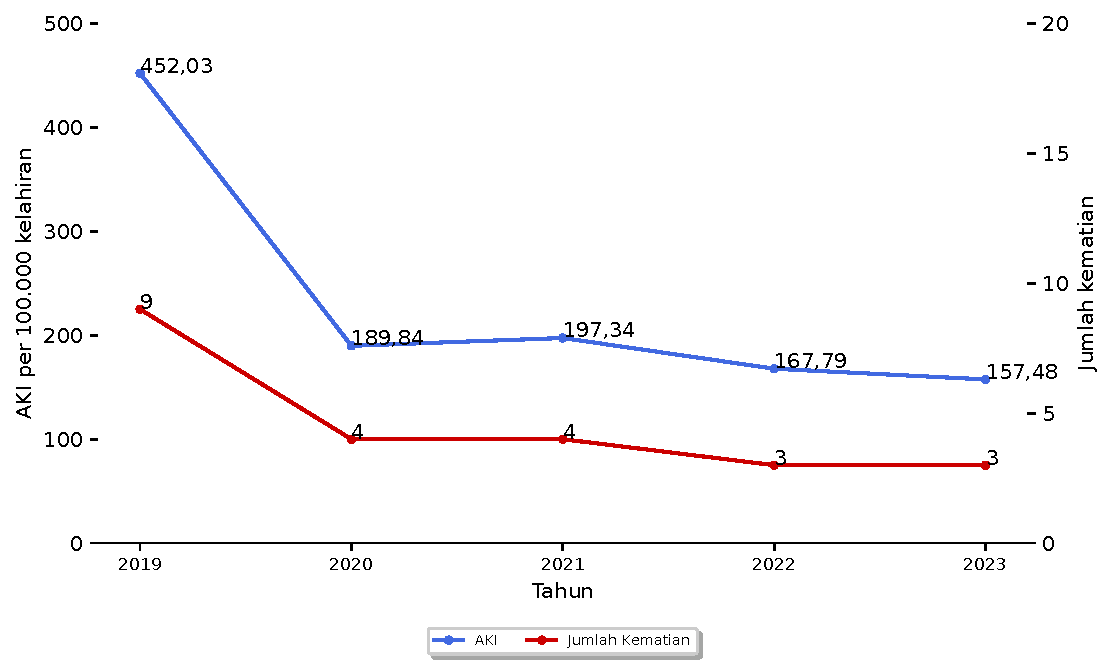
\includegraphics[width=0.85\textwidth]{bab_05/bab_05_02_plotAKI}
    \caption{AKI Kab. Belitung Timur 2019-2023}
    \label{fig:AKI-2019-2023}
\end{figure}

\subsection{Pelayanan Antenatal (K1, K4, dan K6)}
Cakupan kunjungan ibu hamil K-1 adalah cakupan kunjungan ibu hamil yang mendapat pelayanan antenatal sesuai standar (10T) oleh tenaga kesehatan pada masa kehamilan trimester
pertama di satu wilayah kerja pada kurun waktu tertentu. Cakupan ibu hamil K4 adalah cakupan ibu hamil yang mendapatkan pelayanan antenatal sesuai standar (10T) paling sedikit empat kali, dengan distribusi pemberian pelayanan yang dianjurkan adalah minimal satu kali pada trimester pertama, satu kali pada trimester kedua dan dua kali pada trimester ketiga umur kehamilan. Cakupan ibu hamil K6 adalah cakupan ibu hamil yang mendapatkan pelayanan antenatal sesuai standar (10T) paling sedikit enam kali, dengan distribusi pemberian pelayanan yang dianjurkan adalah minimal satu kali pada trimester pertama, dua kali pada trimester kedua dan tiga kali pada trimester ketiga dengan paling sedikit 2 kali oleh dokter pada trimester pertama dan ketiga.

Cakupan K1 dan K4 di Kabupaten Belitung Timur pada tahun \tP adalah sebesar 87,29\% dan 85,56\% (\autoref{fig:Cakupan-K1-K4}), meningkat dari cakupan tahun 2022 sebesar 86,27\% dan 81,52\%(\autoref{fig:Cakupan-K1-K4-2019-2023}).

\begin{figure}[H]
    \centering{}
    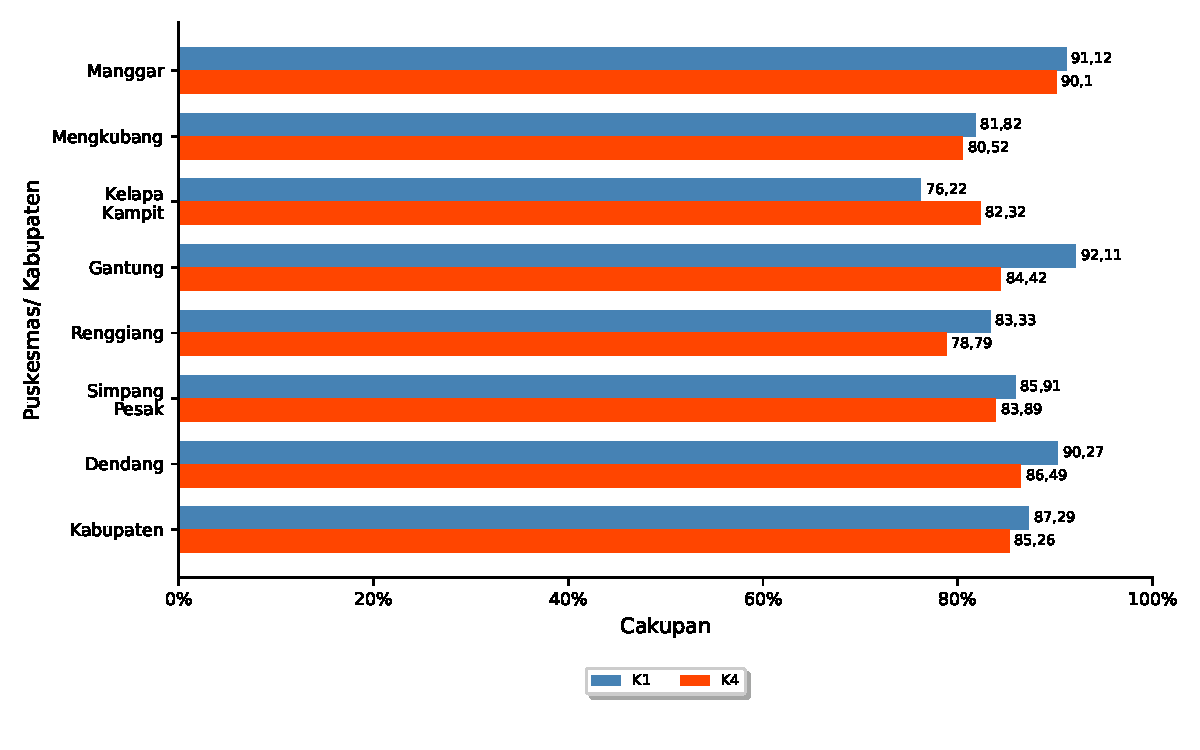
\includegraphics[width=0.9\textwidth]{bab_05/bab_05_03_K1K4}
    \caption{Cakupan K1 dan K4 di Kab. Belitung Timur Tahun \tP per Puskesmas}
    \label{fig:Cakupan-K1-K4}
\end{figure}

\begin{figure}[H]
    \centering{}
    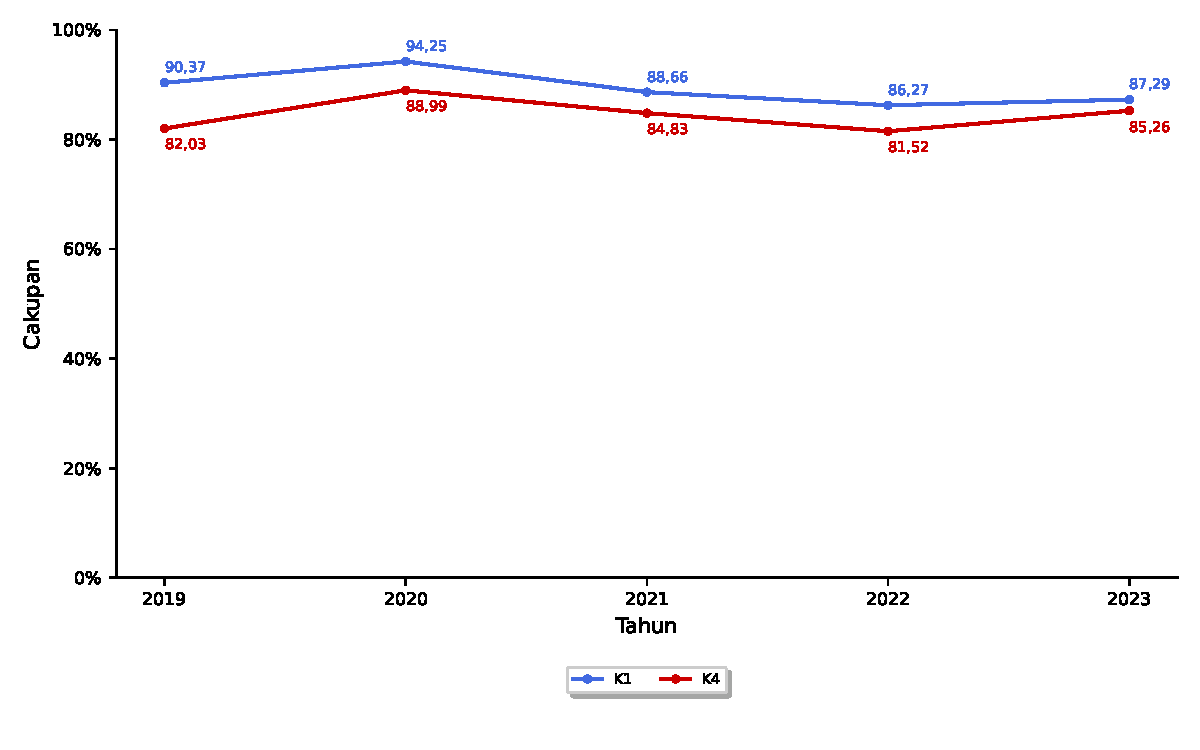
\includegraphics[width=0.85\textwidth]{bab_05/bab_05_03a_plotK1K4}
    \caption{Cakupan K1 dan K4 di Kab. Belitung Timur Tahun 2019-2023}
    \label{fig:Cakupan-K1-K4-2019-2023}
\end{figure}

Cakupan K6 di Kabupaten Belitung Timur pada tahun \tP adalah sebesar 83,37\% (\autoref{fig:Cakupan-K6}).

\begin{figure}[H]
	\centering{}
    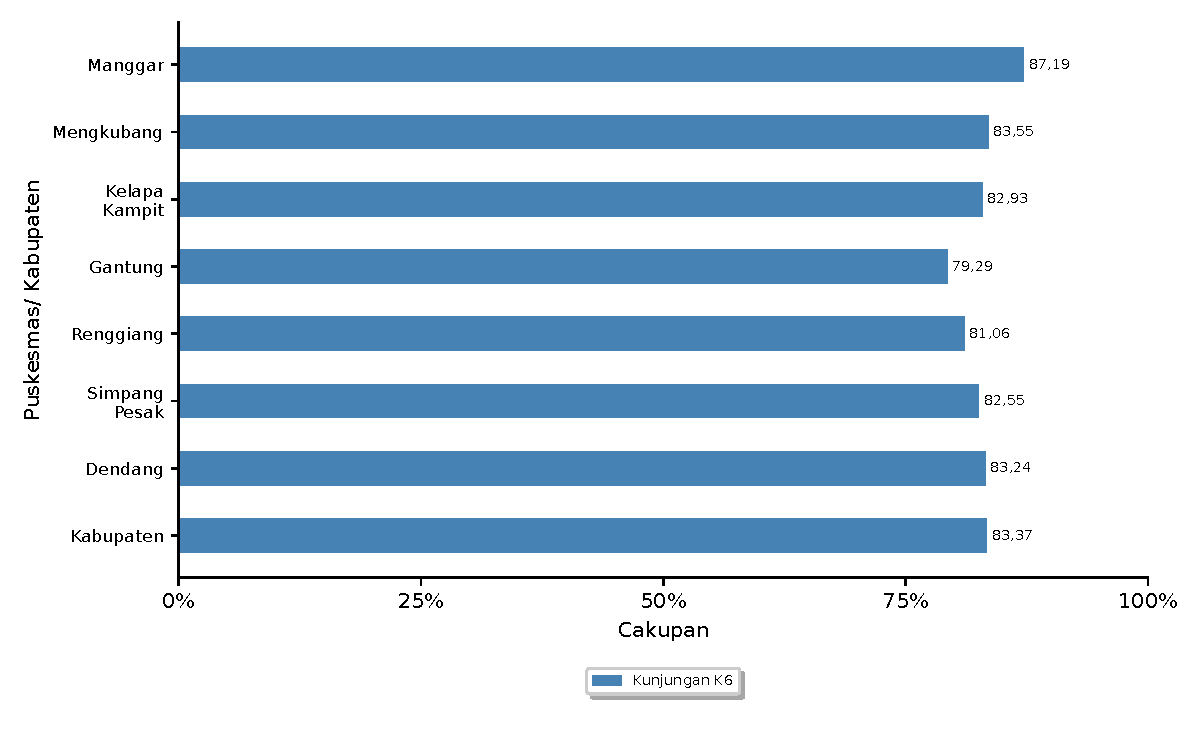
\includegraphics[width=0.9\textwidth]{bab_05/bab_05_03c_K6}
	\caption{Cakupan K6 di Kab. Belitung Timur Tahun \tP per Puskesmas}
	\label{fig:Cakupan-K6}
\end{figure}

\subsection{Imunisasi Td Ibu Hamil}
Peraturan Menteri Kesehatan Nomor 42 Tahun 2013 tentang Penyelenggaraan Imunisasi mengamanatkan bahwa wanita usia subur dan ibu hamil merupakan salah satu kelompok populasi yang menjadi sasaran imunisasi lanjutan.
Imunisasi lanjutan adalah kegiatan yang bertujuan untuk melengkapi imunisasi dasar pada bayi yang diberikan kepada anak batita, anak usia sekolah, dan wanita usia subur termasuk ibu hamil.
Salah satu upaya imunisasi lanjutan yang menyasar ibu hamil adalah imunisasi Td untuk mengendalikan infeksi tetanus yang merupakan salah satu faktor risiko kematian ibu dan kematian bayi.
Infeksi tetanus disebabkan oleh bakteri \emph{Clostridium tetani} sebagai akibat dari proses persalinan yang tidak aman/ steril atau berasal dari luka yang diperoleh ibu hamil sebelum melahirkan.

Cakupan Imunisasi Td pada ibu hamil adalah ang mendapatkan imunisasi Td (Tetanus difteri) dengan interval tertentu (yang dimulai saat dan atau sebelum kehamilan) dengan memperhatikan hasil skrining dan status T.

Cakupan Td5 ibu hamil di kabupaten Belitung Timur tahun \tP yaitu sebesar 74,49\%, sedangkan cakupan Td2+ yaitu sebesar 86,62\% (\autoref{fig:Cakupan-Td}).

\begin{figure}[H]
    \centering{}
    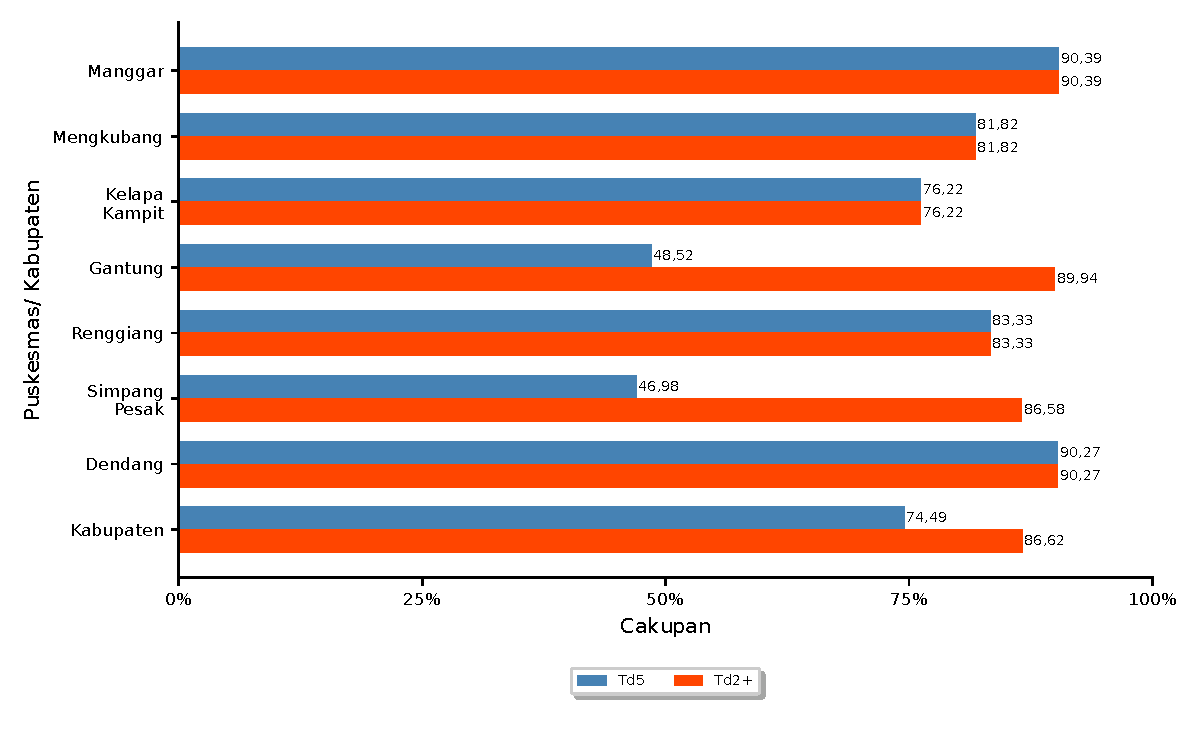
\includegraphics[width=0.85\textwidth]{bab_05/bab_05_04_Td}
    \caption{Cakupan Imunisasi Td Ibu Hamil di Kab. Belitung Timur Tahun \tP per Puskemas}
    \label{fig:Cakupan-Td}
\end{figure}

\subsection{Pemberian Tablet Tambah Darah}
Salah satu komponen pelayanan kesehatan ibu hamil yaitu pemberian suplemen zat besi sebanyak 90 tablet (Fe3).
Zat besi merupakan mineral yang dibutuhkan tubuh untuk membentuk sel darah merah (hemoglobin).
Zat besi memiliki peran vital terhadap pertumbuhan janin.
Selama hamil, asupan zat besi harus ditambah mengingat selama kehamilan, volume darah pada tubuh ibu meningkat.
Sehingga, untuk dapat tetap memenuhi kebutuhan ibu dan menyuplai makanan serta oksigen pada janin melalui plasenta, dibutuhkan asupan zat besi yang lebih banyak.

Cakupan ibu hamil mendapat TTD adalah persentase ibu hamil yang mendapatkan Tablet Tambah Darah (TTD) sekurangnya mengandung zat besi setara dengan 60 mg besi elemental dan 0,4 mg asam folat yang disediakan oleh pemerintah minimal 90 tablet selama masa kehamilan. Cakupan ibu hamil mengonsumsi TTD adalah persentase ibu hamil yang mengonsumsi Tablet Tambah Darah (TTD) sekurangnya mengandung zat besi setara dengan 60 mg besi elemental dan 0,4 mg asam folat yang disediakan oleh pemerintah minimal 90 tablet selama masa kehamilan.

Cakupan ibu hamil mendapat TTD di Kabupaten Belitung Timur pada tahun \tP adalah sebesar 82,02\% (\autoref{fig:Cakupan-TTD}).

\begin{figure}[H]
    \centering
    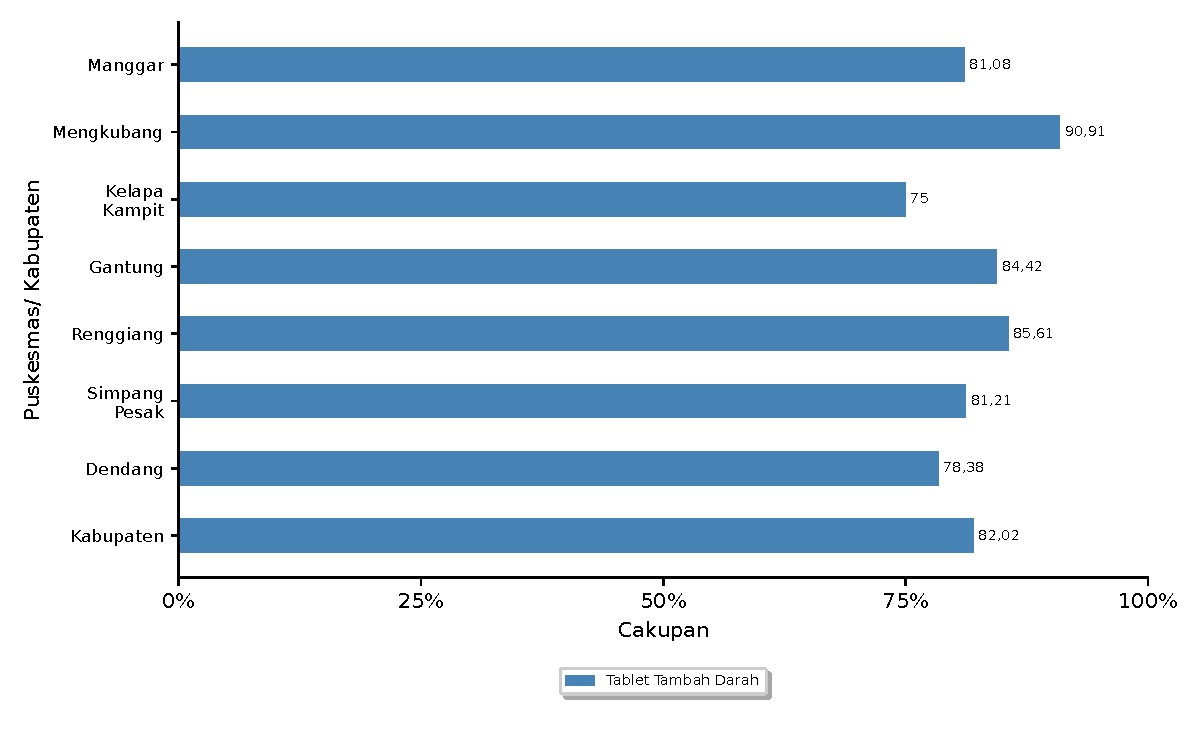
\includegraphics[width=0.9\textwidth]{bab_05/bab_05_05_TTD}
    \caption{Cakupan Pemberian TTD di Kab. Belitung Timur Tahun \tP per Puskesmas}
    \label{fig:Cakupan-TTD}
\end{figure}


\subsection{Pertolongan Persalinan oleh Tenaga Kesehatan dengan Kompetensi Kebidanan}
Salah satu upaya menekan angka kematian ibu dan bayi yaitu dengan mendorong upaya persalinan dilakukan oleh tenaga kesehatan dengan kompetensi kebidanan di fasilitas pelayanan kesehatan.

Cakupan persalinan di fasilitas pelayanan kesehatan adalah cakupan ibu bersalin yang mendapatkan pelayanan persalinan sesuai standar di fasilitas pelayanan kesehatan di satu wilayah kerja pada kurun waktu tertentu.

Cakupan persalinan di fasilitas pelayanan kesehatan di Kabupaten Belitung Timur pada tahun \tP yaitu sebesar 90,04\% (\autoref{fig:Cakupan-Persalinan-Fasyankes}).

\begin{figure}[H]
    \centering
    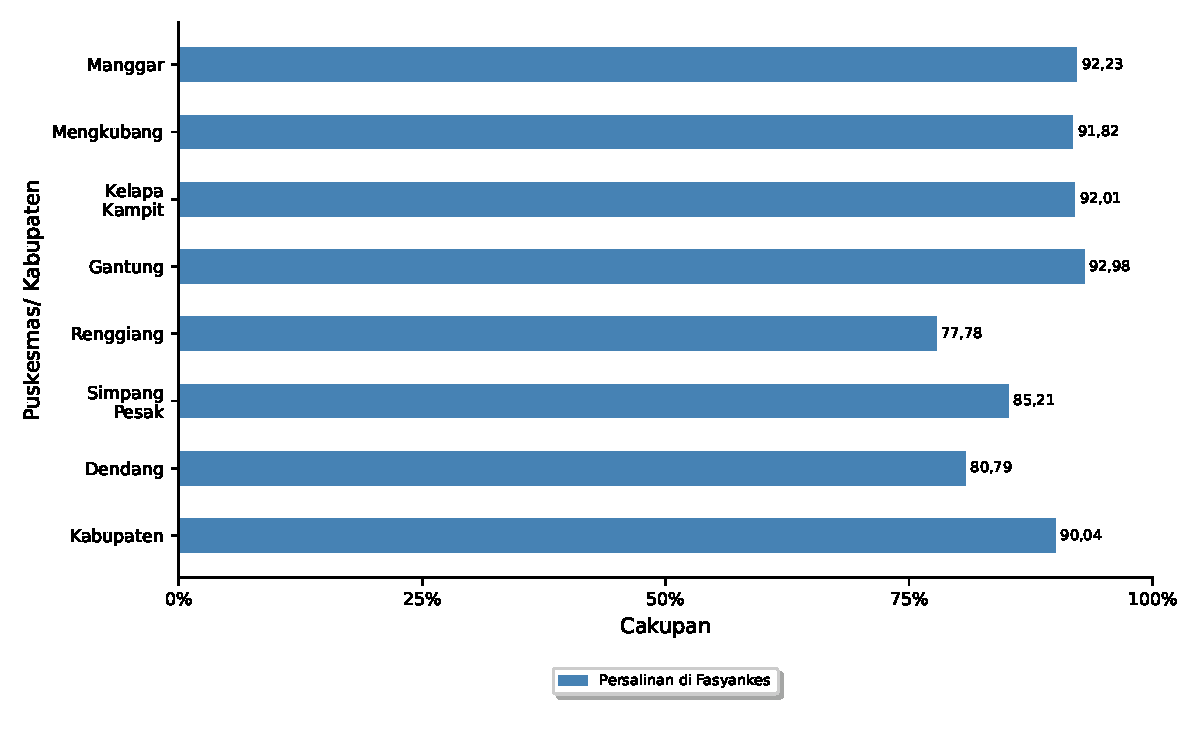
\includegraphics[width=0.9\textwidth]{bab_05/bab_05_05b_salinFasyankes.pdf}
    \caption{Cakupan Persalinan di Fasyankes di Kab. Belitung Timur Tahun \tP per Puskesmas}
    \label{fig:Cakupan-Persalinan-Fasyankes}
\end{figure}

\subsection{Pelayanan Kesehatan Nifas}
Masa nifas dimulai dari enam jam sampai dengan 42 hari pasca persalinan.
Pelayanan kesehatan nifas adalah pelayanan kepada ibu nifas sesuai standar sedikitnya 3 kali, yaitu kunjungan nifas ke-1 pada 6 jam setelah persalinan s.d 3 hari; kunjungan nifas ke-2 hari ke 4 s/d hari ke 28 setelah persalinan, kunjungan nifas ke-3 hari ke 29 s/d hari ke 42 setelah persalinan.

Cakupan pelayanan nifas KF Lengkap adalah cakupan pelayanan kepada ibu pada masa 6 jam sampai dengan 42 hari pasca bersalin sesuai standar paling sedikit 4 kali dengan distribusi waktu 6 jam sampai hari ke-2 (KF1), hari ke-3 sampai hari ke-7 (KF2), hari ke 8 sampai ke-28 (KF3) dan hari ke-29 sampai ke-42 (KF4) setelah bersalin di suatu wilayah kerja pada kurun waktu tertentu.

Cakupan pelayanan kesehatan nifas di Kabupaten Belitung Timur pada tahun \tP sebesar 89,28\% (\autoref{fig:Cakupan-Yankes-Nifas}).%, menurun dari cakupan tahun 2020 sebesar 97,43\%.

\begin{figure}[H]
    \centering{}
    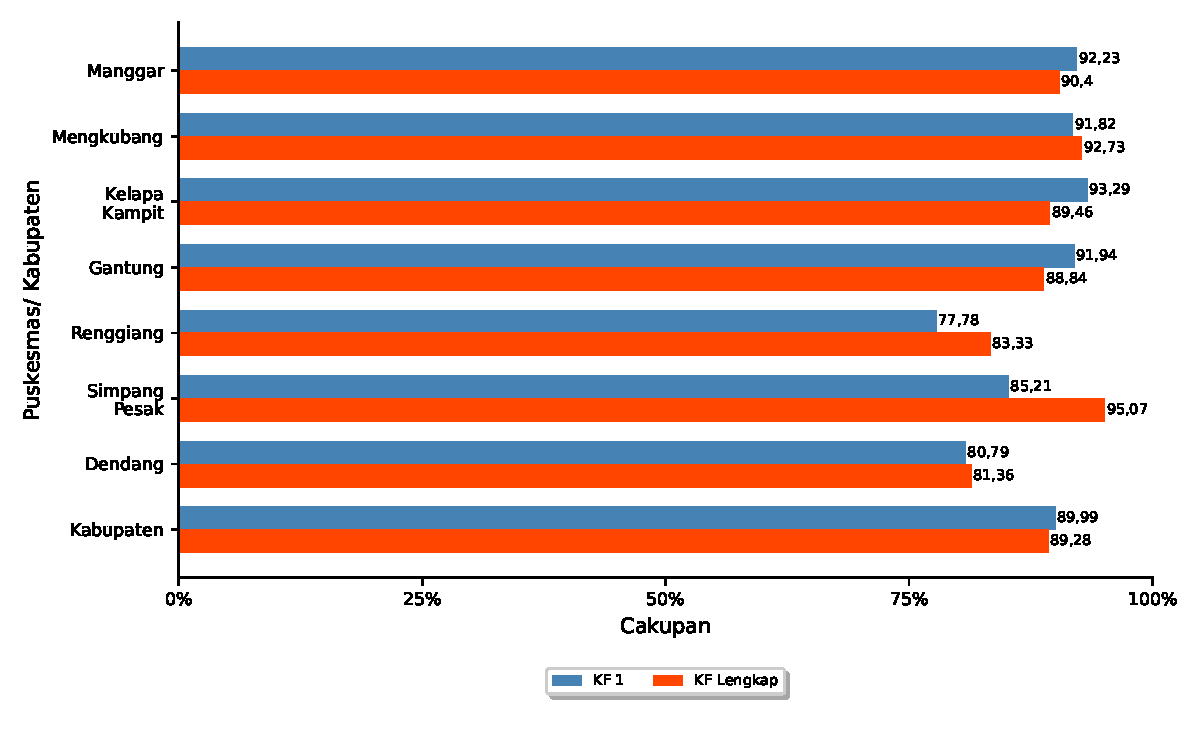
\includegraphics[width=0.9\textwidth]{bab_05/bab_05_05c_layanNifas}
    \caption{Cakupan Pelayanan Kesehatan Nifas di Kab. Belitung Timur Tahun \tP per Puskesmas}
    \label{fig:Cakupan-Yankes-Nifas}
\end{figure}

Cakupan ibu nifas mendapat vitamin A adalah cakupan ibu yang baru melahirkan atau nifas yang mendapatkan kapsul vitamin A 200.000 SI sehingga bayinya akan memperoleh vitamin A melalui ASI di satu wilayah kerja pada kurun waktu tertentu.
Cakupan ibu nifas mendapat vitamin A di Kabupaten Belitung Timur pada tahun \tP sebesar 89,57\% (\autoref{fig:Cakupan-Nifas-VitA}).

\begin{figure}[H]
    \centering{}
    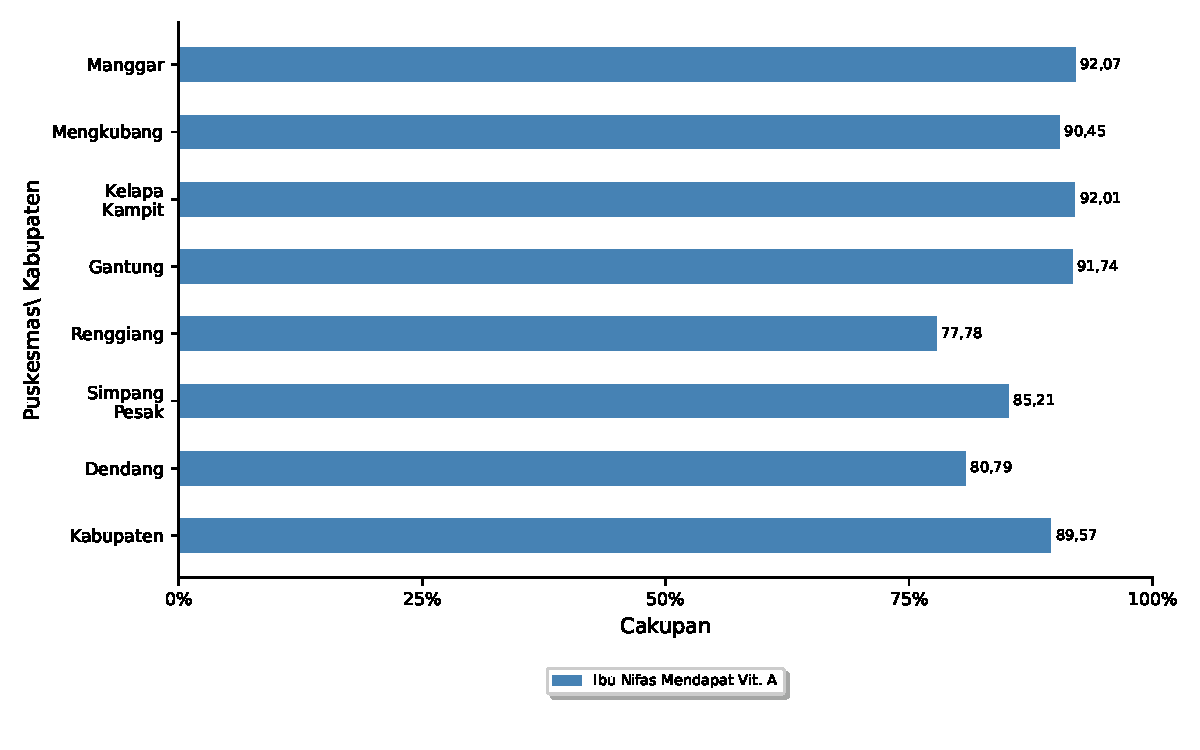
\includegraphics[width=0.9\textwidth]{bab_05/bab_05_05d_nifasVitA}
    \caption{Cakupan Ibu Nifas Mendapat Vitamin A di Kab. Belitung Timur Tahun \tP per Puskesmas}
    \label{fig:Cakupan-Nifas-VitA}
\end{figure}

\subsection{Penanganan Komplikasi Kebidanan}
Komplikasi kebidanan adalah kesakitan pada ibu hamil, ibu bersalin, ibu nifas yang dapat mengancam jiwa ibu dan/atau bayi. Sebagai salah satu faktor penyebab kematian ibu dan bayi, perlu dilakukan penanganan komplikasi kebidanan sebagai upaya menekan angka kematian ibu dan bayi.

Cakupan penanganan komplikasi kebidanan di Kabupaten Belitung Timur pada tahun \tP adalah sebesar 112,21\%,
%menurun dari cakupan tahun 2020 sebesar 133,97\% (\autoref{fig:Cakupan-Komplikasi-Kebidanan}).

\begin{figure}[H]
    \centering
    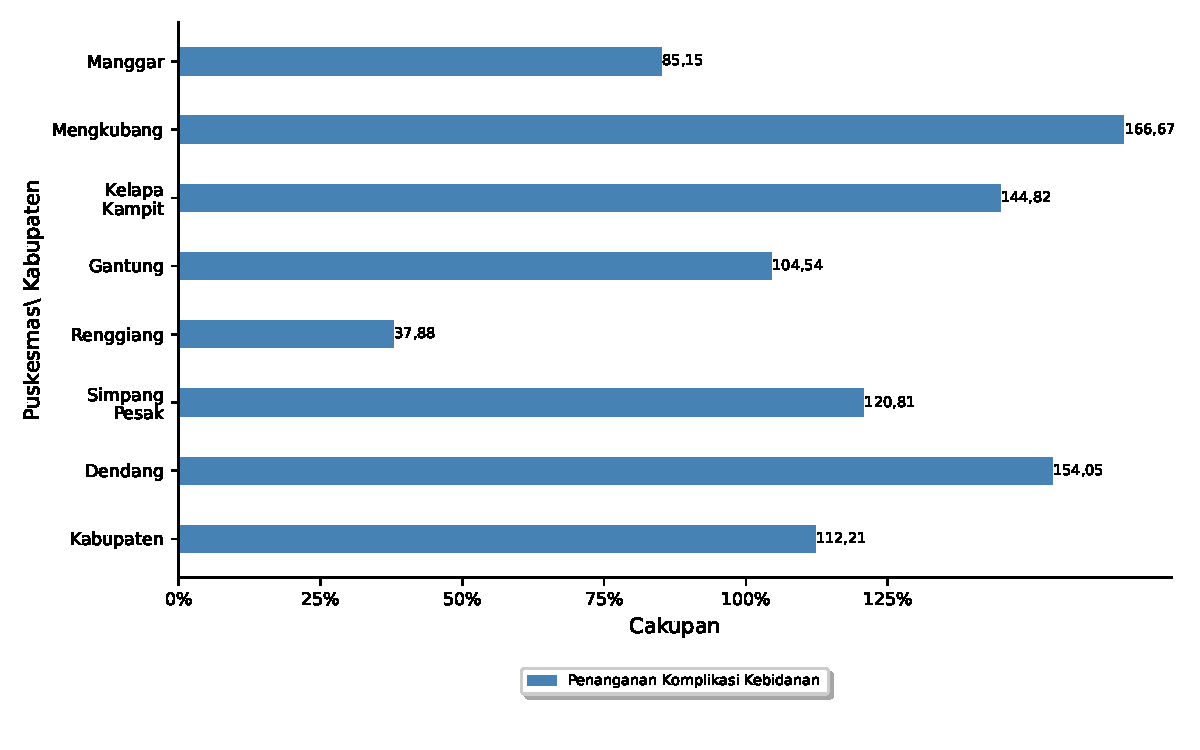
\includegraphics[width=0.9\textwidth]{bab_05/bab_05_05e_komplikasiKebidanan}
    \caption{Cakupan Penanganan Komplikasi Kebidanan di Kab. Belitung Timur Tahun \tP per Puskesmas}
    \label{fig:Cakupan-Komplikasi-Kebidanan}
\end{figure}


\subsection{Cakupan Peserta Keluarga Berencana}
Keluarga Berencana (KB) adalah upaya mengatur kelahiran anak, jarak dan usia ideal melahirkan, mengatur kehamilan, melalui promosi, perlindungan, dan bantuan sesuai dengan hak reproduksi untuk mewujudkan keluarga yang berkualitas. Program KB bertujuan untuk:
\begin{itemize}
 \item mengatur kehamilan yang diinginkan;
 \item menjaga kesehatan dan menurunkan angka kematian ibu, bayi dan anak;
 \item meningkatkan akses dan kualitas informasi, pendidikan, konseling, dan pelayanan keluarga berencana dan kesehatan reproduksi;
 \item meningkatkan partisipasi dan kesertaan pria dalam praktek keluarga berencana; dan
 \item mempromosikan penyusuan bayi sebagai upaya untuk menjarangkan jarak kehamilan.
\end{itemize}
Diharapkan dengan program KB akan dapat meningkatkan kualitas keluarga agar dapat timbul rasa aman, tenteram, dan harapan masa depan yang lebih baik dalam mewujudkan kesejahteraan lahir dan kebahagiaan batin.

\subsubsection{Cakupan peserta KB Aktif}
Peserta KB aktif adalah peserta KB baru dan lama yang masih aktif memakai kontrasepsi terus-menerus untuk menunda, menjarangkan kehamilan atau yang mengakhiri kesuburan. Cakupan peserta KB aktif di Kabupaten Belitung Timur pada tahun \tP adalah sebesar 79,03\% (\autoref{fig:Cakupan-KB-aktif-a} \& ~\autoref{fig:Cakupan-KB-aktif-b}). Metode KB yang paling banyak dipilih oleh peserta KB aktif adalah KB Suntik sebanyak 60,77 \% (\autoref{fig:Cakupan-KB-aktif-c}).

\begin{figure}[H]
    \centering
    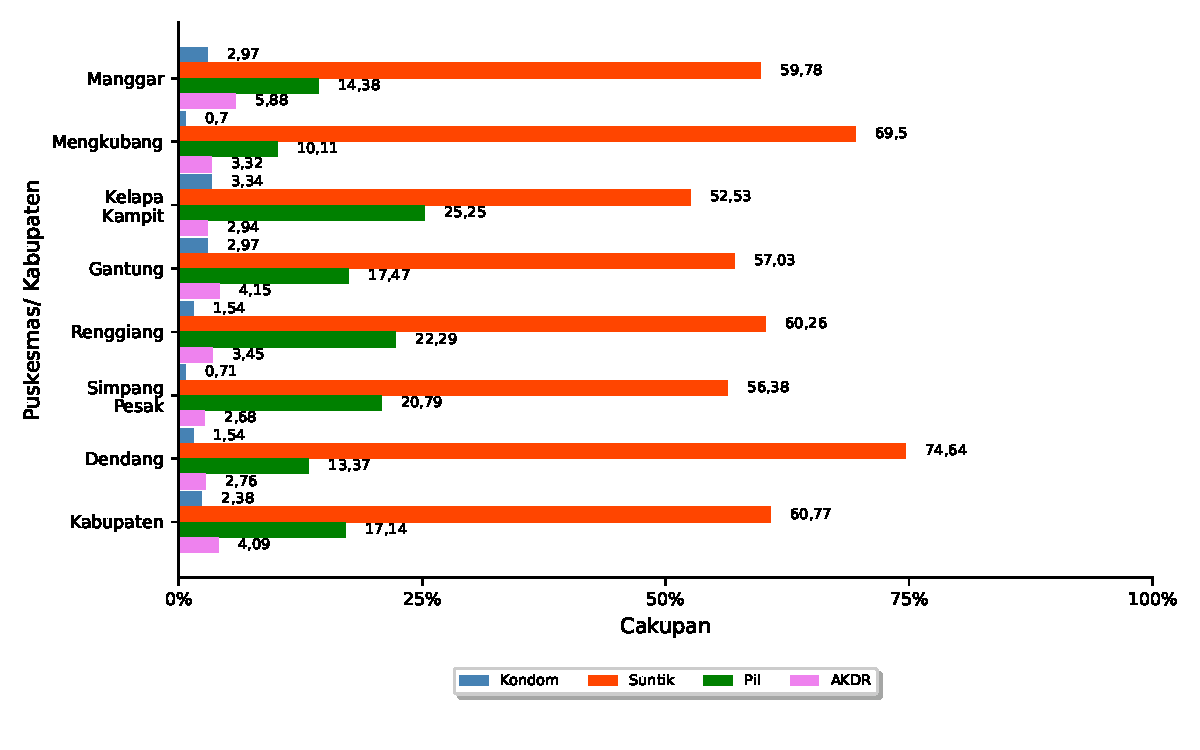
\includegraphics[width=0.9\textwidth]{bab_05/bab_05_06_KBaktif_a}
    \caption{Cakupan Peserta KB Aktif di Kab. Belitung Timur Tahun \tP per Puskesmas}
    \label{fig:Cakupan-KB-aktif-a}
\end{figure}

\begin{figure}[H]
    \centering
    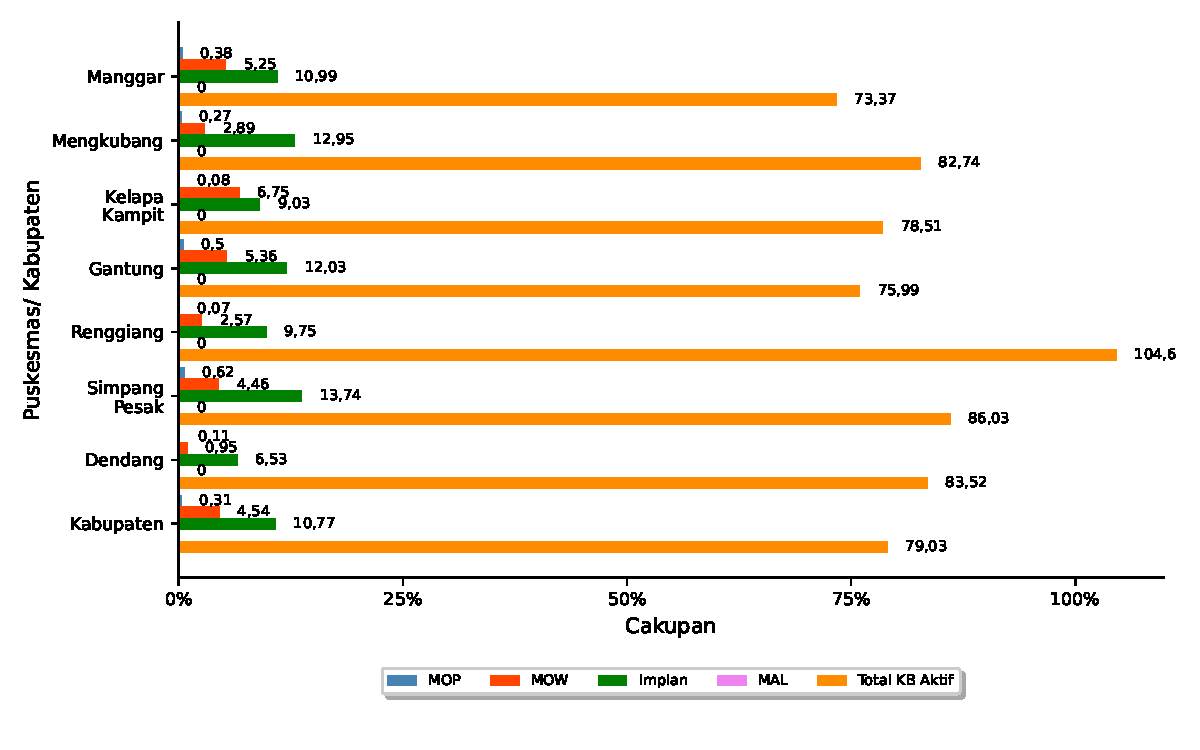
\includegraphics[width=0.9\textwidth]{bab_05/bab_05_06_KBaktif_b}
    \caption{Cakupan Peserta KB Aktif di Kab. Belitung Timur Tahun \tP per Puskesmas (lanj.)}
    \label{fig:Cakupan-KB-aktif-b}
\end{figure}

\begin{figure}[H]
    \centering
    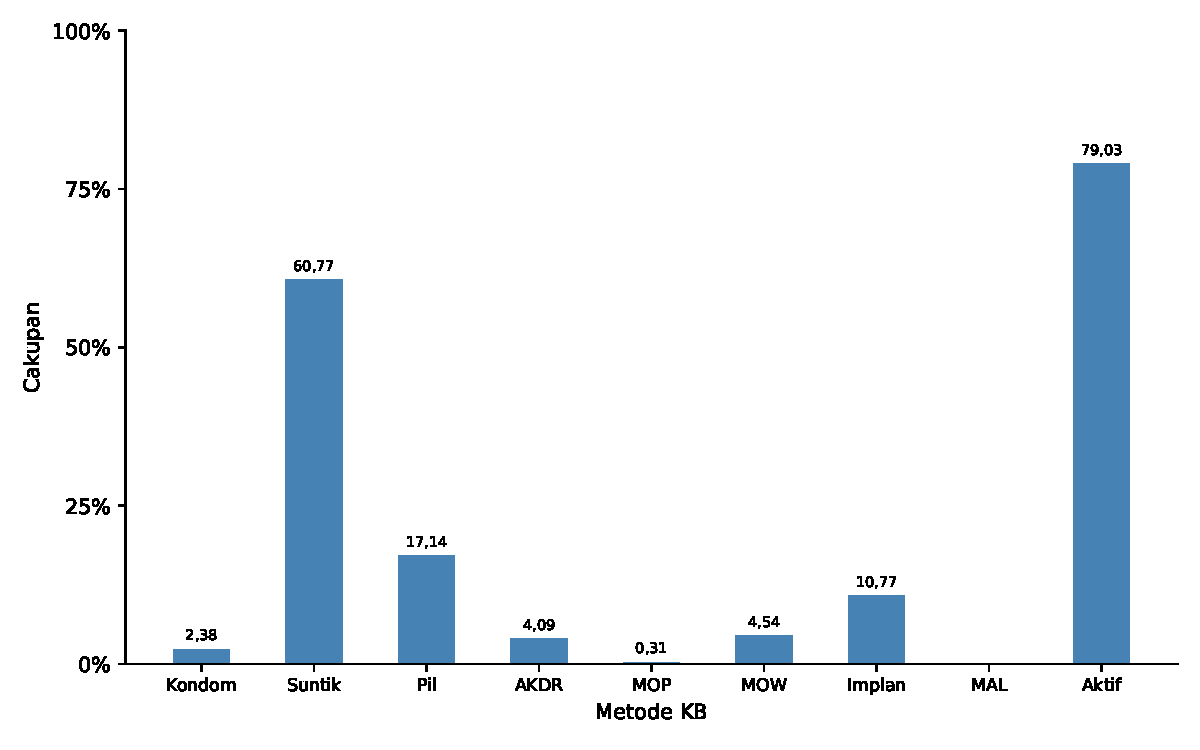
\includegraphics[width=0.9\textwidth]{bab_05/bab_05_06_KBaktif_c}
    \caption{Cakupan Metode Yang Digunakan Peserta KB Aktif di Kab. Belitung Timur Tahun \tP}
    \label{fig:Cakupan-KB-aktif-c}
\end{figure}

\subsubsection{Pasangan Usia Subur dengan status 4T dan ALKI}
Pasangan Usia Subur(PUS) dengan status 4 Terlalu (4T) adalah PUS dimana istrinya memenuhi minimal salah satu kriteria 4 Terlalu (4T), yaitu :
\begin{enumerate}
	\item berusia kurang dari 20 tahun;
	\item berusia lebih dari 35 tahun;
	\item telah memiliki anak hidup lebih dari 3 orang;atau
	\item jarak kelahiran antara satu anak dengan lainnya kurang dari 2 tahun
\end{enumerate}

Cakupan PUS dengan status 4T yang menjadi peserta KB aktif di Kabupaten Belitung Timur pada tahun \tP  adalah sebesar 14,16\% (\autoref{fig:Cakupan-4T-ALKI-menjadi-KB-Aktif}).

Pasangan Usia Subur(PUS) dengan ALKI adalah PUS yang istrinya mengalami salah satu dari gejala: Anemia, Lingkar Lengan Atas < 23,5, penyakit kronis, atau Infeksi Menular Seksual (IMS).
Penyakit kronis yang dimaksud terdiri dari Diabetes Melitus, Hipertensi, jantung, ginjal, auto imun, Hepatitis B, Thyroid, TORCH, hiperkoagulasi, stroke, Thalasemia, Hemofilia, kanker, masalah kesehatan jiwa, HIV, TBC, dan Malaria.

Cakupan PUS dengan ALKI yang menjadi peserta KB aktif di Kabupaten Belitung Timur pada tahun \tP  adalah sebesar 3,96\% (\autoref{fig:Cakupan-4T-ALKI-menjadi-KB-Aktif}).

\begin{figure}[H]
	\centering
	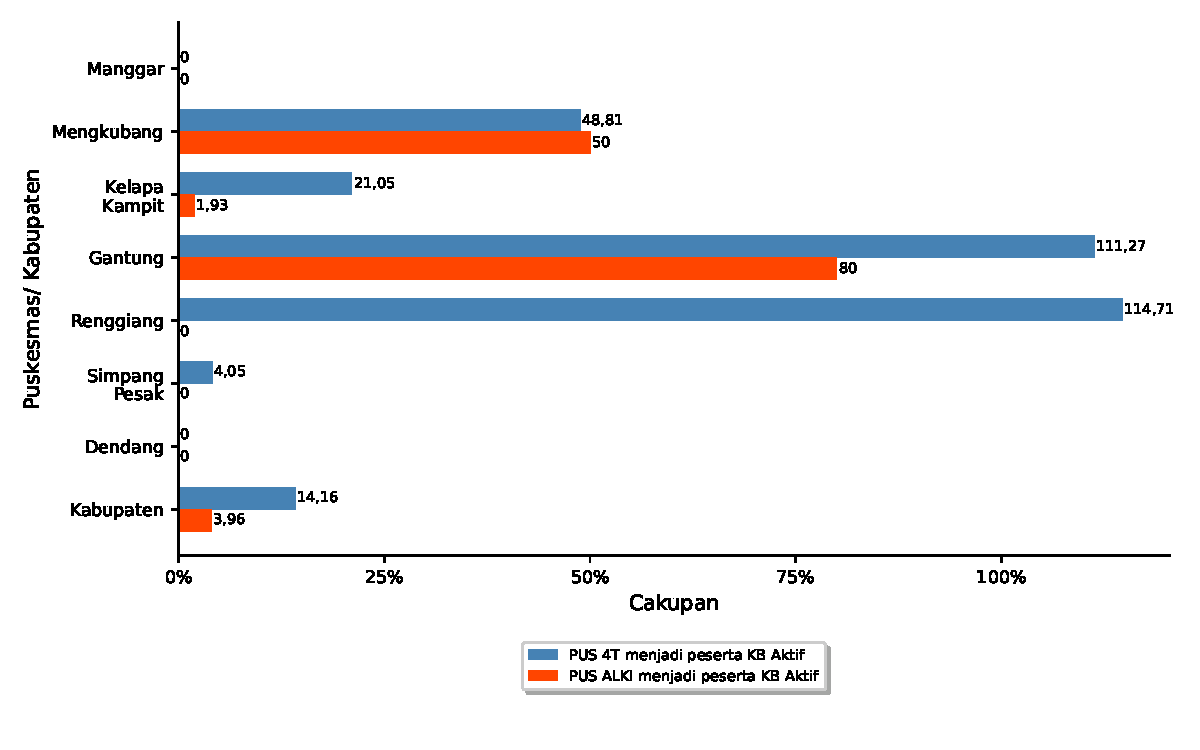
\includegraphics[width=0.9\textwidth]{bab_05/bab_05_06a_KB4TALKI}
	\caption{Cakupan PUS Dengan Status 4T dan ALKI Menjadi Peserta KB Aktif di Kab. Belitung Timur Tahun \tP}
	\label{fig:Cakupan-4T-ALKI-menjadi-KB-Aktif}
\end{figure}

\subsubsection{Cakupan peserta KB Pasca Persalinan}
Peserta KB Pasca Persalinan adalah Pasangan Usia Subur (PUS) yang memakai kontrasepsi pada masa pasca persalinan (0-42 hari setelah melahirkan). Cakupan peserta KB pasca persalinan di Kabupaten Belitung Timur pada tahun \tP adalah sebesar 73,98\% dari jumlah ibu bersalin(\autoref{fig:Cakupan-KB-pascaSalin-a} \& ~\autoref{fig:Cakupan-KB-pascaSalin-b}). Metode KB yang paling banyak dipilih oleh PUS di masa pasca persalinan adalah KB Suntik sebanyak 46,84 \% (\autoref{fig:Cakupan-KB-pascaSalin-c}).

\begin{figure}[H]
    \centering
    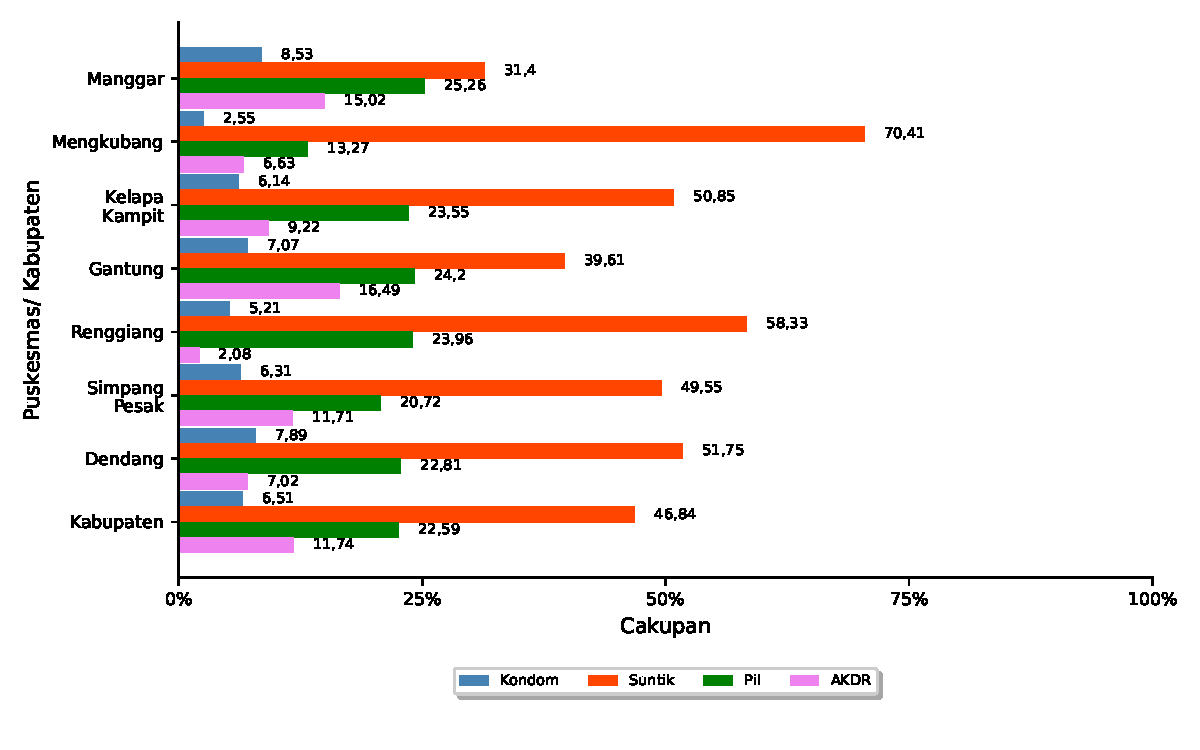
\includegraphics[width=0.85\textwidth]{bab_05/bab_05_07_KBpascaSalin_a}
    \caption{Cakupan Peserta KB Pasca Persalinan di Kab. Belitung Timur Tahun \tP per Puskesmas}
    \label{fig:Cakupan-KB-pascaSalin-a}
\end{figure}

\begin{figure}[H]
    \centering
    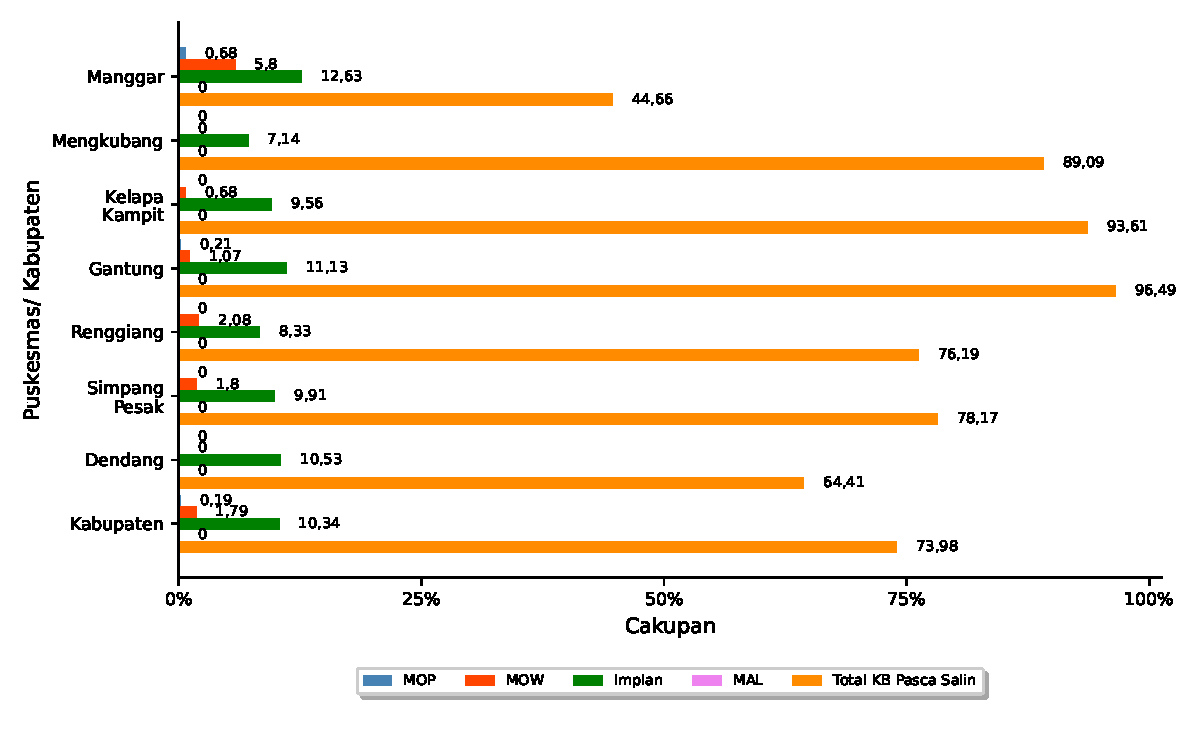
\includegraphics[width=0.85\textwidth]{bab_05/bab_05_07_KBpascaSalin_b}
    \caption{Cakupan Peserta KB Pasca Persalinan di Kab. Belitung Timur Tahun \tP per Puskesmas (lanj.)}
    \label{fig:Cakupan-KB-pascaSalin-b}
\end{figure}

\begin{figure}[H]
    \centering
    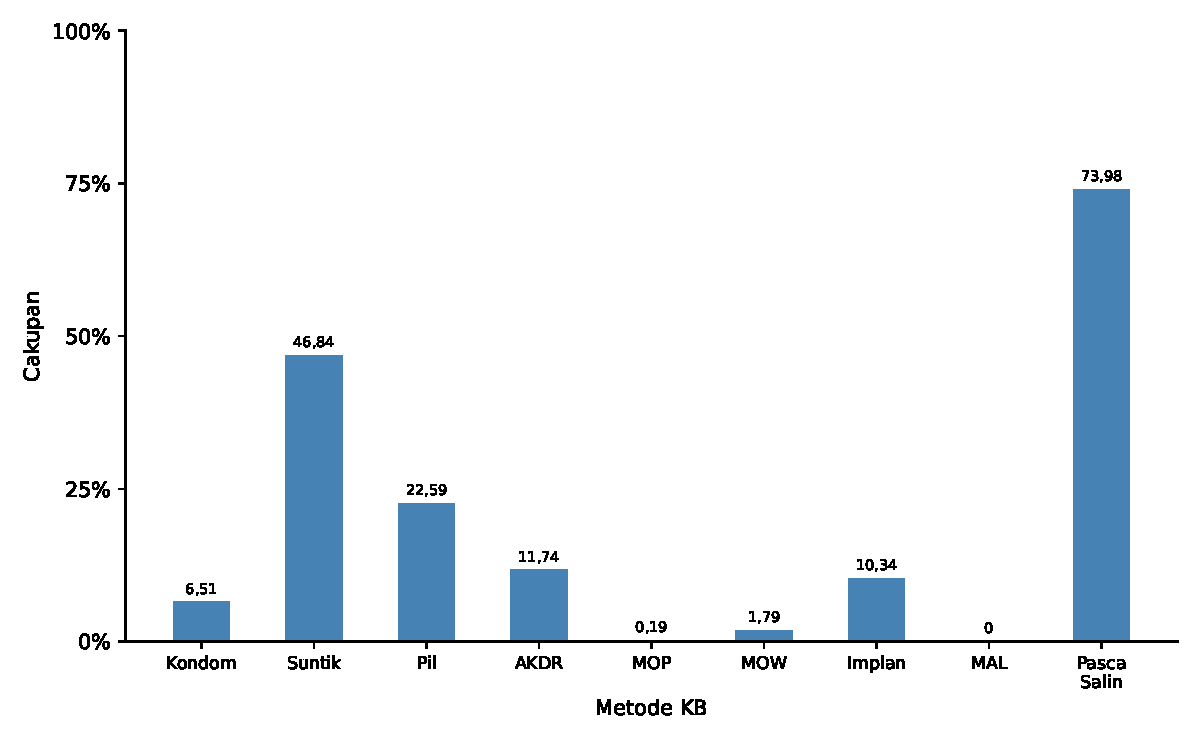
\includegraphics[width=0.9\textwidth]{bab_05/bab_05_07_KBpascaSalin_c}
    \caption{Cakupan Metode Yang Digunakan Peserta KB pasca Persalinan di Kab. Belitung Timur Tahun \tP}
    \label{fig:Cakupan-KB-pascaSalin-c}
\end{figure}

\section{KESEHATAN ANAK}
\subsection{Angka Kematian Neonatal (AKN)}
Kematian Neonatal adalah kematian yang terjadi pada bayi usia sampai dengan 28 hari tetapi bukan disebabkan oleh kecelakaan, bencana, cedera atau bunuh diri. Angka Kematian Neonatal per 1.000 kelahiran hidup adalah jumlah bayi usia sampai dengan 28 hari yang meninggal di suatu wilayah pada kurun waktu tertentu per 1.000 jumlah kelahiran hidup di wilayah dan pada kurun waktu yang sama.

Jumlah Kematian Neonatus yang terjadi di Kabupaten Belitung Timur sepanjang tahun \tP berjumlah 14 kematian (\autoref{fig:Jumlah-Kematian-Neonatal}). Angka Kematian Neonatal (AKN) pada tahun \tP sebesar 7,35 per 1.000 kelahiran hidup, mengalami penurunan dari tahun 2022 sebesar 8,39 per 1.000 kelahiran hidup (\autoref{fig:AKN-2019-2023}).

\begin{figure}[H]
    \centering{}
    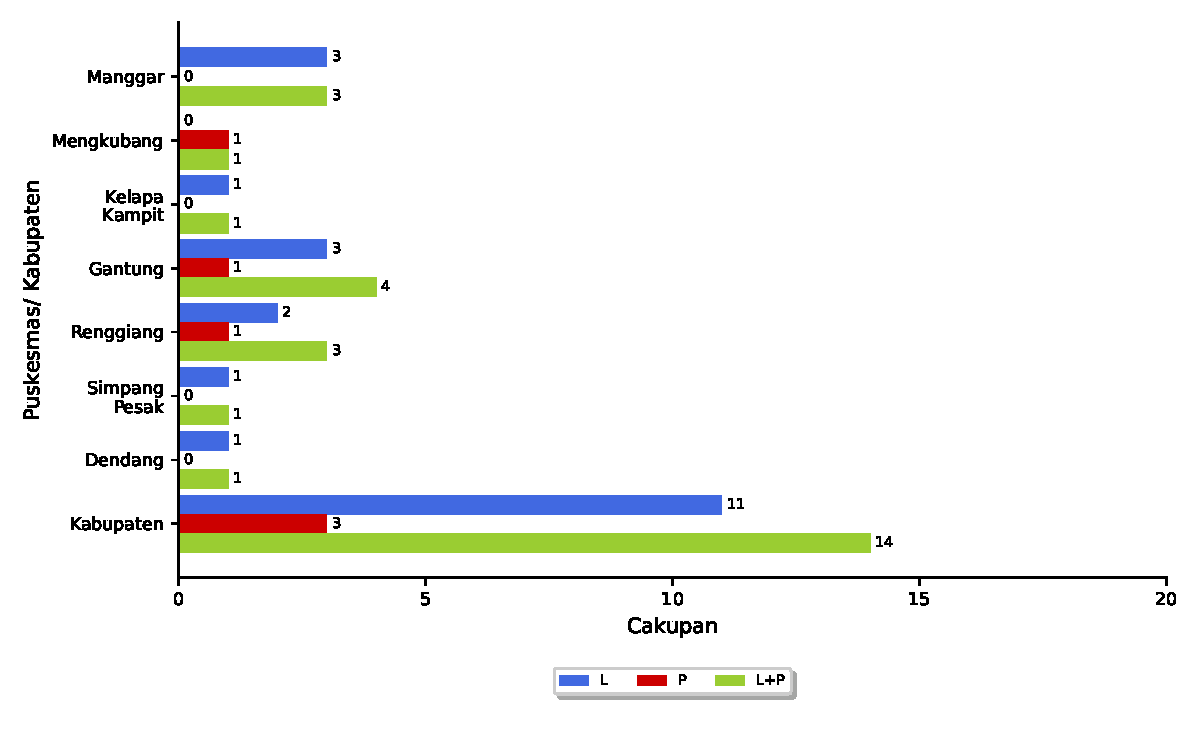
\includegraphics[width=0.85\textwidth]{bab_05/bab_05_09_kematianNeonatal}
    \caption{Jumlah Kematian Neonatal di Kab. Belitung Timur Tahun \tP per Puskesmas}
    \label{fig:Jumlah-Kematian-Neonatal}
\end{figure}

\begin{figure}[H]
    \centering{}
    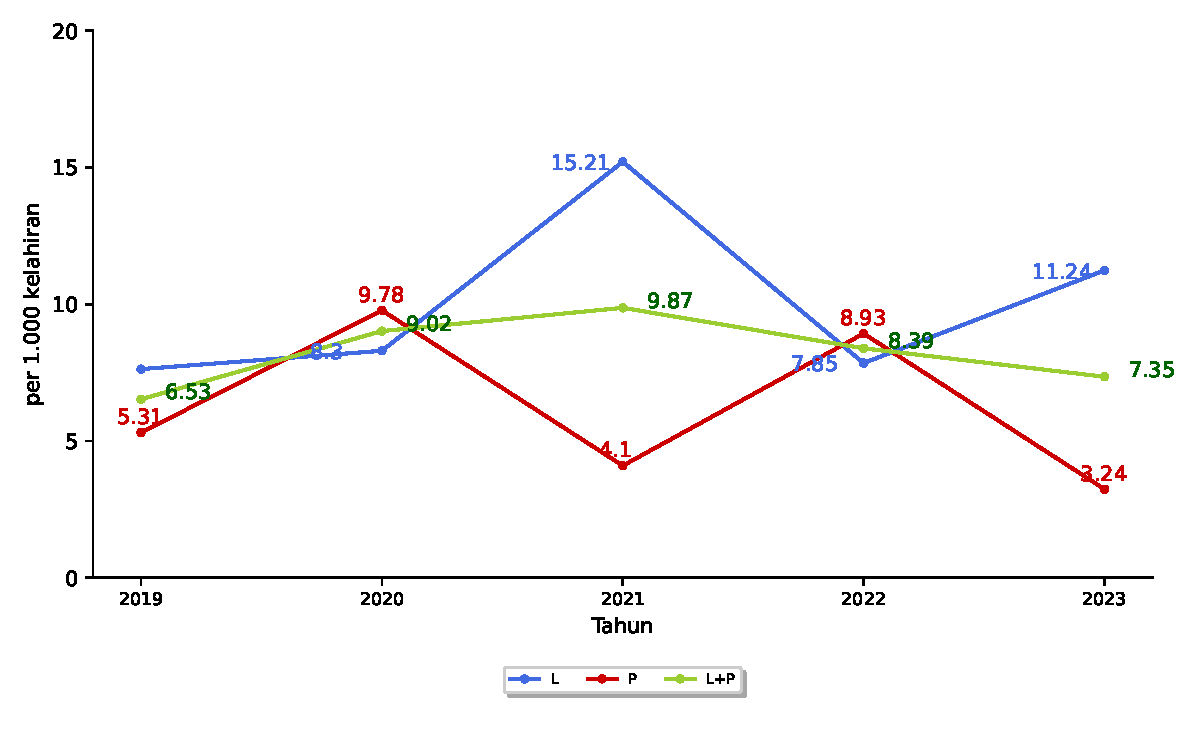
\includegraphics[width=0.85\textwidth]{bab_05/bab_05_09_plotNeonatal}
    \caption{AKN Kab. Belitung Timur Tahun 2019-2023}
    \label{fig:AKN-2019-2023}
\end{figure}


\subsection{Angka Kematian Bayi (AKB)}
Kematian Bayi adalah kematian yang terjadi pada seorang bayi yang usianya sebelum mencapai satu tahun (usia 0-11 bulan, mencakup neonatal dan postnatal) tetapi bukan disebabkan oleh kecelakaan, bencana, cedera atau bunuh diri. Angka Kematian Bayi per 1.000 kelahiran hidup adalah jumlah bayi usia sampai dengan 11 bulan yang meninggal di suatu wilayah pada kurun waktu tertentu per 1.000 jumlah kelahiran hidup di wilayah dan pada kurun waktu yang sama.

Jumlah Kematian Bayi yang terjadi di Kabupaten Belitung Timur sepanjang tahun \tP berjumlah 17 kematian (\autoref{fig:Jumlah-Kematian-Bayi}). Angka Kematian Bayi (AKB) pada tahun \tP adalah sebesar 8,92 per 1.000 kelahiran hidup, mengalami penurunan dari AKB tahun 2022 sebesar 12,30 per 1.000 kelahiran hidup (\autoref{fig:AKB-2019-2023}).

\begin{figure}[H]
    \centering{}
    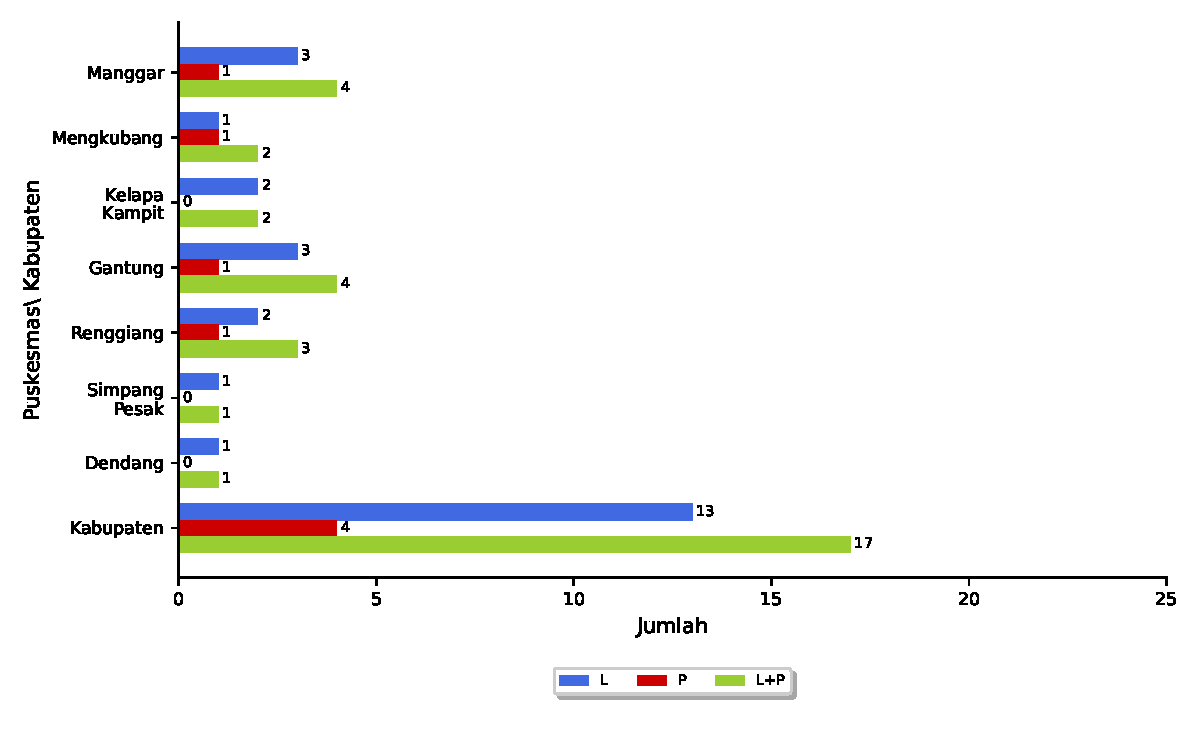
\includegraphics[width=0.85\textwidth]{bab_05/bab_05_10_kematianBayi}
    \caption{Jumlah Kematian Bayi di Kab. Belitung Timur Tahun \tP per Puskesmas}
    \label{fig:Jumlah-Kematian-Bayi}
\end{figure}

\begin{figure}[H]
    \centering{}
    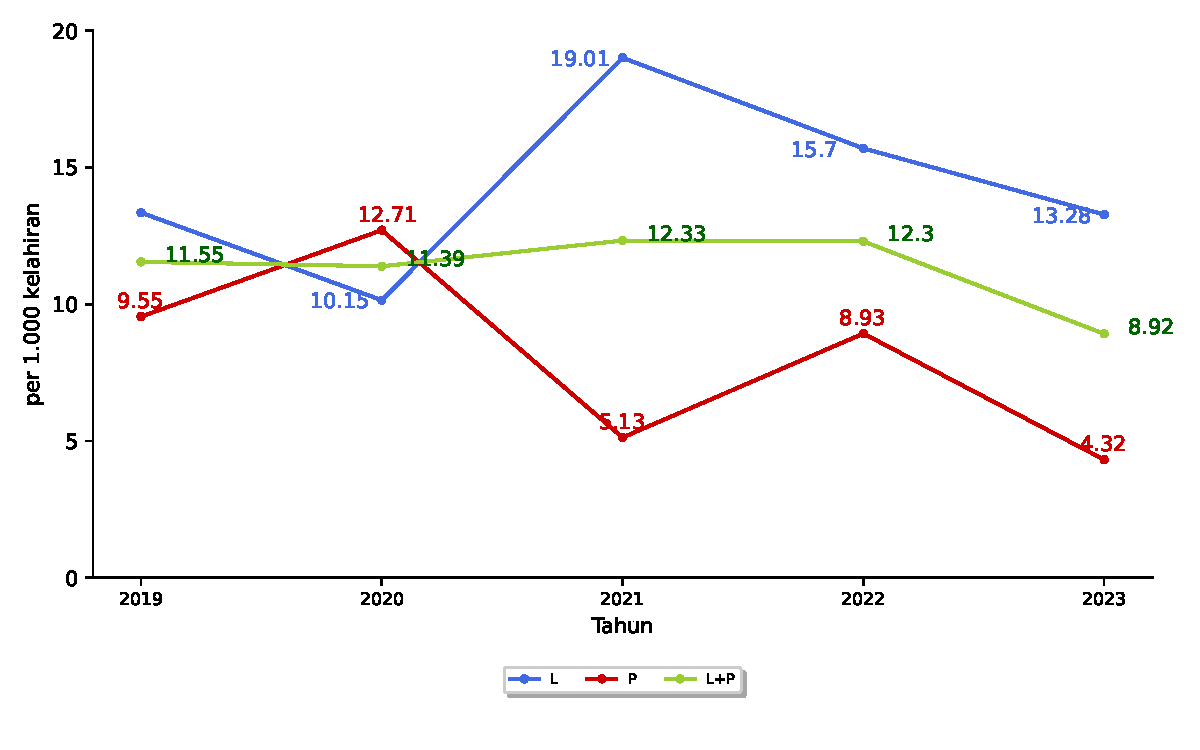
\includegraphics[width=0.85\textwidth]{bab_05/bab_05_10_plotBayi}
    \caption{AKB Kab. Belitung Timur Tahun 2019-2023}
    \label{fig:AKB-2019-2023}
\end{figure}


\subsection{Angka Kematian Balita (AKBA)}
Kematian Balita adalah kematian yang terjadi pada bayi/anak usia 0 - 59 bulan (bayi + anak balita) tetapi bukan disebabkan oleh kecelakaan, bencana, cedera atau bunuh diri. Angka Kematian Balita (AKBA) adalah jumlah balita usia 59 bulan (mencakup bayi dan anak balita) yang meninggal di suatu wilayah pada kurun waktu tertentu
per 1.000 jumlah kelahiran hidup di wilayah pada kurun waktu yang sama.

Jumlah Kematian Balita yang terjadi di Kabupaten Belitung Timur sepanjang tahun \tP berjumlah 19 kematian (\autoref{fig:Jumlah-Kematian-Balita}). Angka Kematian Balita (AKBA) pada tahun \tP sebesar 9,97 per 1.000 kelahiran hidup, mengalami penurunan dari AKBA tahun 2022 sebesar 14,54 per 1.000 kelahiran hidup (\autoref{fig:AKBA-2019-2023}).

\begin{figure}[H]
    \centering{}
    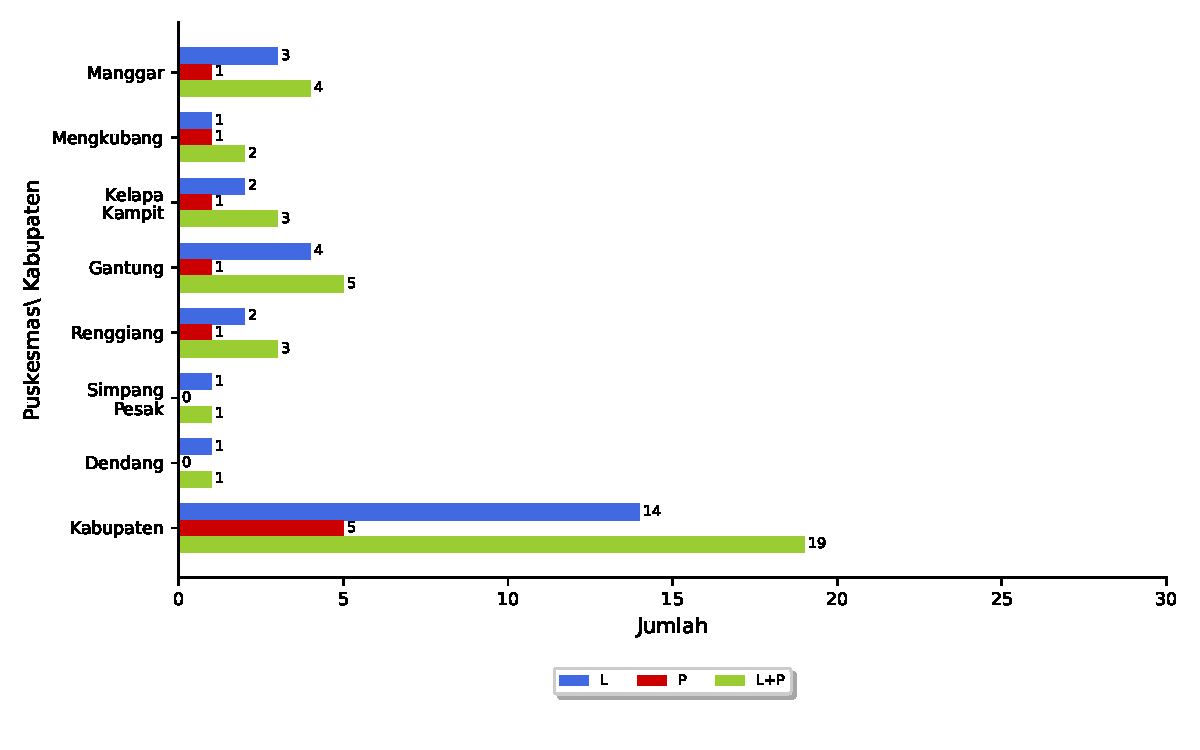
\includegraphics[width=0.85\textwidth]{bab_05/bab_05_11_kematianBalita}
    \caption{Jumlah Kematian Balita di Kabupaten Belitung Timur Tahun \tP per Puskesmas}
    \label{fig:Jumlah-Kematian-Balita}
\end{figure}

\begin{figure}[H]
    \centering{}
    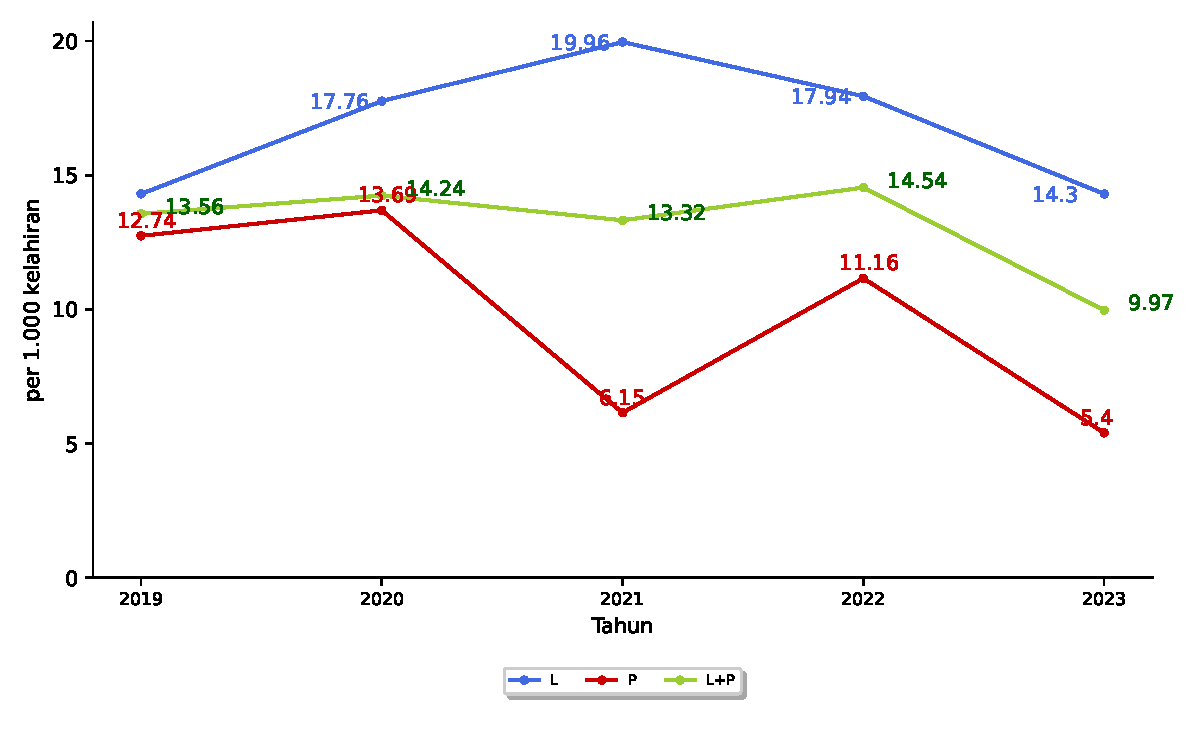
\includegraphics[width=0.8\textwidth]{bab_05/bab_05_11_plotBalita}
    \caption{AKABA Kabupaten Belitung Timur 2019-2023}
    \label{fig:AKBA-2019-2023}
\end{figure}

\begin{figure}[H]
    \centering{}
    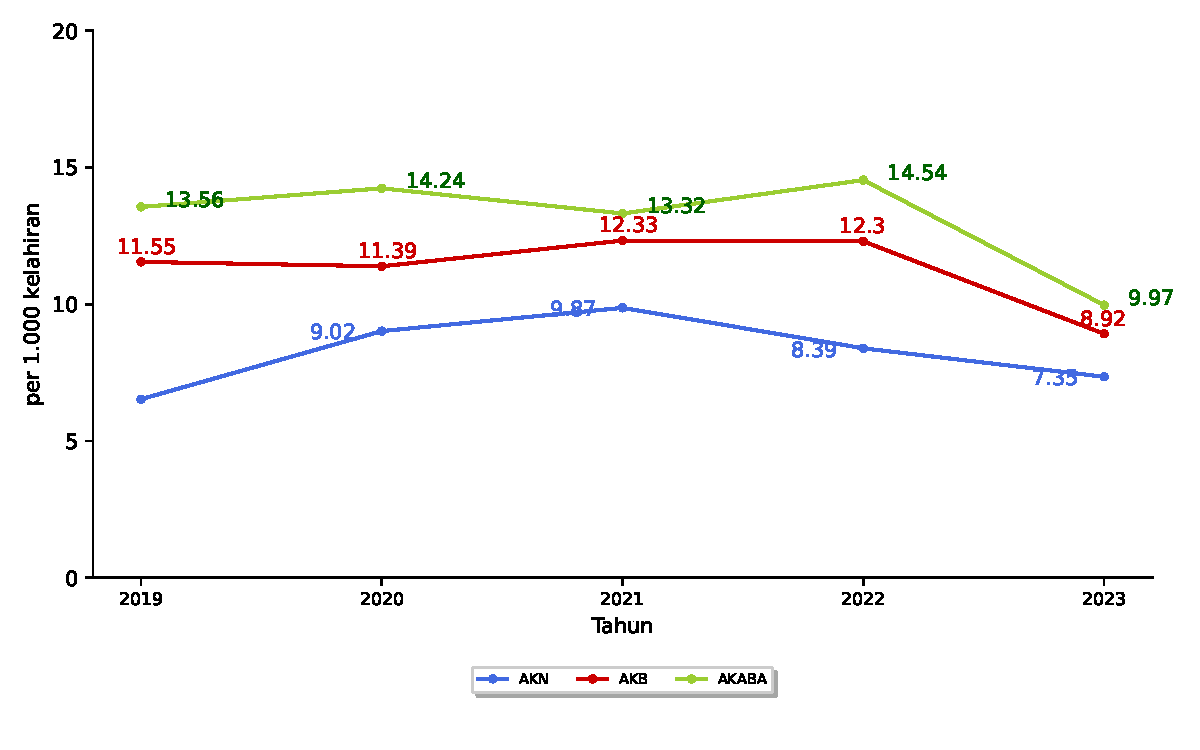
\includegraphics[width=0.8\textwidth]{bab_05/bab_05_11a_plotNeoBayiBalita}
    \caption{AKN, AKB dan AKBA Kabupaten Belitung Timur 2019-2023}
    \label{fig:AKN-AKB-AKBA-2019-2023}
\end{figure}

\subsection{Penanganan Komplikasi Neonatal}
Komplikasi neonatal adalah neonatal dengan penyakit dan kelainan yang
dapat menyebabkan kesakitan, kecacatan, dan kematian neonatus dengan
komplikasi seperti BBLR (berat badan lahir rendah < 2500 gr), asfiksia, infeksi, tetanus neonatorum, kelainan kongenital, Covid 19, dan lain-lain
seperti ikterus, hipotermia, trauma lahir, sindroma gangguan pernafasan. Penanganan neonatal dengan komplikasi adalah
penanganan terhadap neonatal sakit dan atau neonatal dengan kelainan
atau komplikasi/kegawatdaruratan yang mendapat pelayanan sesuai standar
oleh tenaga kesehatan terlatih di seluruh sarana pelayanan kesehatan.
Pelayanan sesuai standar antara lain sesuai dengan standar MTBM, Manajemen
Asfiksia Bayi Baru Lahir, Manajemen Bayi Berat Lahir Rendah, pedoman
pelayanan neonatal essensial di tingkat pelayanan kesehatan dasar,
PONED, PONEK atau standar operasional pelayanan lainnya.

Cakupan penanganan komplikasi neonatal di Kabupaten Belitung Timur
pada tahun \tP adalah sebesar 56,22\%.
%menurun dari cakupan tahun2020 sebesar 78,26\% (\autoref{fig:Pelayanan-Komplikasi-Neonatal}).

\begin{figure}[H]
    \centering
    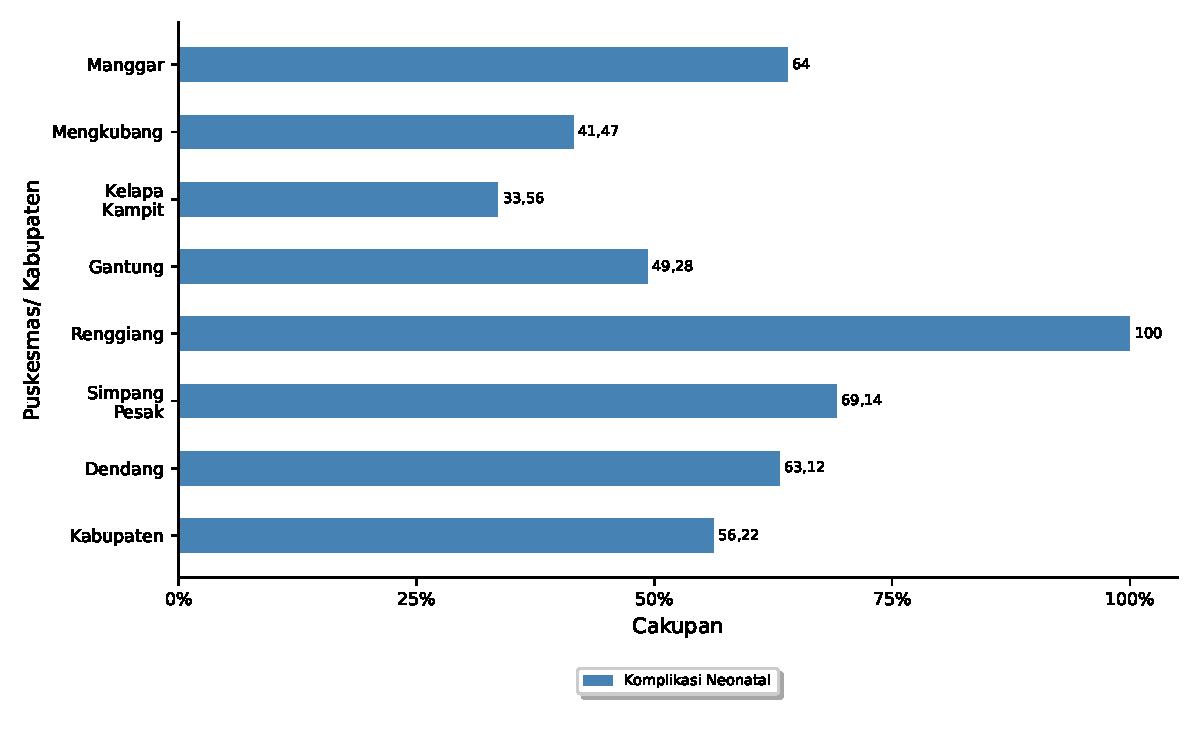
\includegraphics[width=0.85\textwidth]{bab_05/bab_05_12_komplikasiNeonatal}
    \caption{Cakupan Penanganan Komplikasi Neonatal di Kab. Belitung Timur Tahun \tP per Puskesmas}
    \label{fig:Pelayanan-Komplikasi-Neonatal}
\end{figure}


\subsection{Berat Badan Bayi Lahir Rendah (BBLR) dan Bayi Prematur}
Berat Badan Bayi Lahir Rendah adalah berat badan bayi kurang dari
2500 gram. BBLR dibedakan menjadi 2 (dua) kategori yaitu BBLR karena
prematur (kurang dari 37 minggu) dan BBLR karena \emph{Intrauterine Growth Restriction}(IUGR), yaitu bayi yang lahir cukup bulan tetapi berat badannya kurang.

Pada tahun \tP, tercatat bahwa Berat Badan Bayi Lahir Rendah adalah berjumlah
146 kasus atau 7,66\% dari jumlah kelahiran hidup (\autoref{fig:Distribusi-BBLR}).
%menurun dari cakupan tahun 2021 sebesar 5,53\%.

\begin{figure}[H]
  \centering
  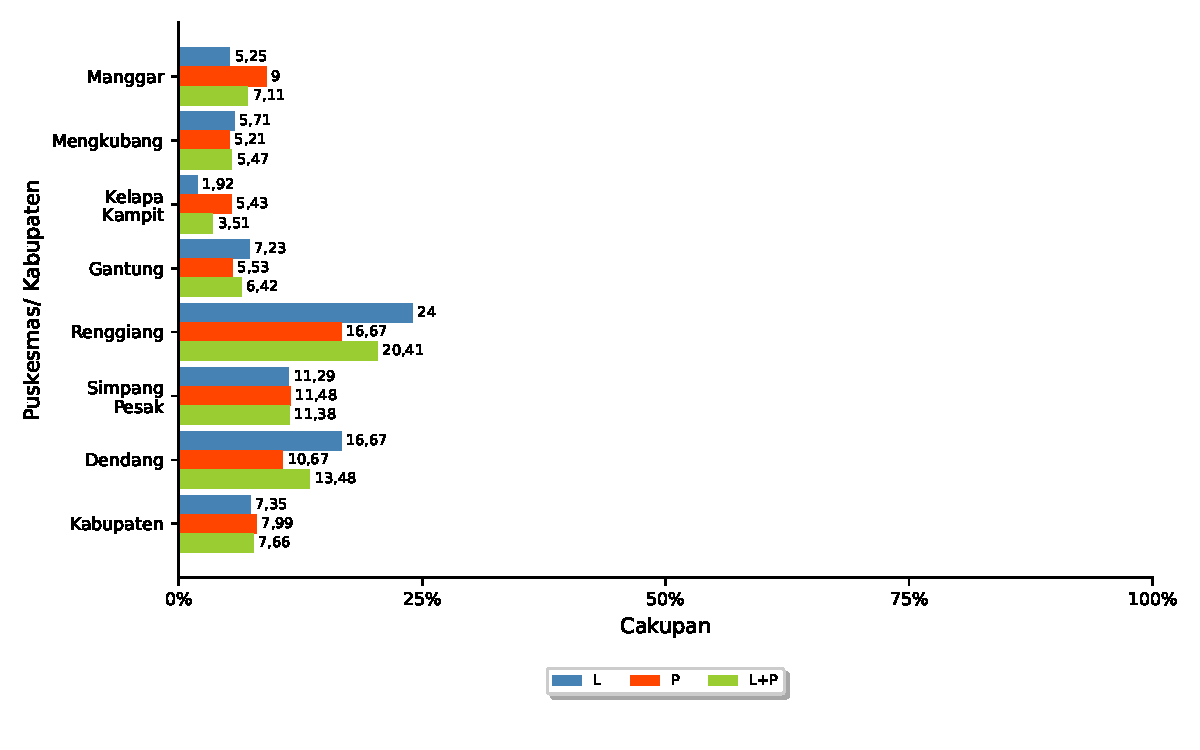
\includegraphics[width=0.85\textwidth]{bab_05/bab_05_13_BBLR}
  \caption{Sebaran BBLR di Kab. Belitung Timur Tahun \tP per Puskesmas}
  \label{fig:Distribusi-BBLR}
\end{figure}

Pada tahun \tP, tercatat bahwa Bayi Lahir Prematur adalah berjumlah
137 kasus atau 6,80\% dari jumlah kelahiran hidup (\autoref{fig:Distribusi-Prematur}).

\begin{figure}[H]
	\centering
	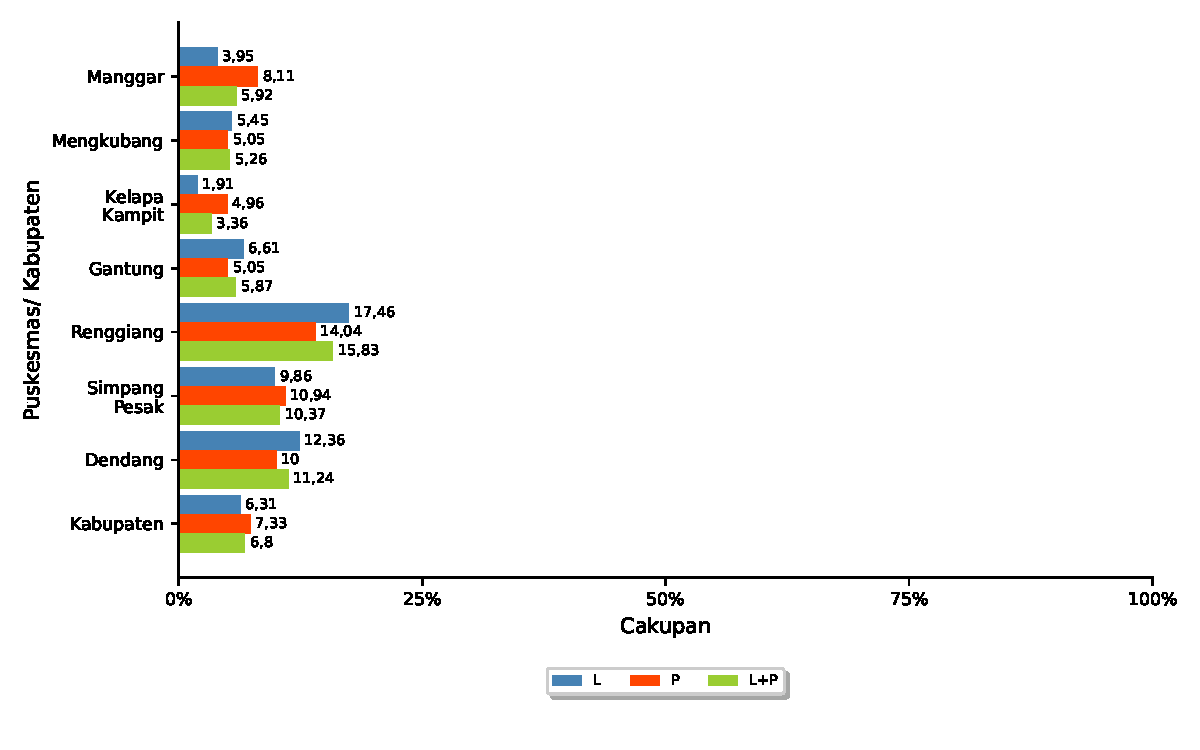
\includegraphics[width=0.85\textwidth]{bab_05/bab_05_13a_Prematur}
	\caption{Sebaran Bayi Lahir Prematur di Kab. Belitung Timur Tahun \tP per Puskesmas}
	\label{fig:Distribusi-Prematur}
\end{figure}

\subsection{Pelayanan Kesehatan Neonatal}
Neonatus adalah bayi baru lahir yang berusia sampai dengan 28 hari.
Pada masa tersebut terjadi perubahan yang sangat besar dari kehidupan
di dalam rahim dan terjadi pematangan organ hampir pada semua sistem.
Beberapa upaya kesehatan dilakukan untuk mengendalikan risiko pada
kelompok ini di antaranya dengan mengupayakan agar persalinan dapat
dilakukan oleh tenaga kesehatan di fasilitas kesehatan serta menjamin
tersedianya pelayanan kesehatan sesuai standar pada kunjungan bayi
baru lahir.

Indikator yang menggambarkan upaya kesehatan yang dilakukan untuk
mengurangi risiko kematian pada periode neonatal yaitu cakupan KN1
dan KN Lengkap. KN1 adalah pelayanan kunjungan neonatal pertama pada
6-48 jam setelah lahir sesuai standar di satu wilayah kerja. KN Lengkap
yaitu pelayanan kunjungan neonatal lengkap, minimal 3 kali yaitu 1
kali pada usia 6 - 48 jam, 1 kali pada 3 - 7 hari, dan 1 kali pada
8 - 28 hari sesuai standar.

%Cakupan penanganan KN1 di Kabupaten Belitung Timur
%pada tahun \tP sebesar 100,00\%, meningkat
%dari cakupan tahun 2019 sebesar 99,90\%. Sedangkan cakupan penanganan KN Lengkap di Kabupaten Belitung Timur
%pada tahun \tP 98,67\%, menurun
%dari cakupan tahun 2019 sebesar 99,60\% (\autoref{fig:Cakupan-KN1-KNlengkap} dan \autoref{fig:KN1-KNlengkap-2016-2020}).

Cakupan penanganan KN1 di Kabupaten Belitung Timur pada tahun \tP sebesar 94,25\%.
Sedangkan cakupan penanganan KN Lengkap di Kabupaten Belitung Timur pada tahun \tP sebesar 94,30\% (\autoref{fig:Cakupan-KN1-KNlengkap}

% dan \autoref{fig:KN1-KNlengkap-2016-2020}).

\begin{figure}[H]
    \centering
    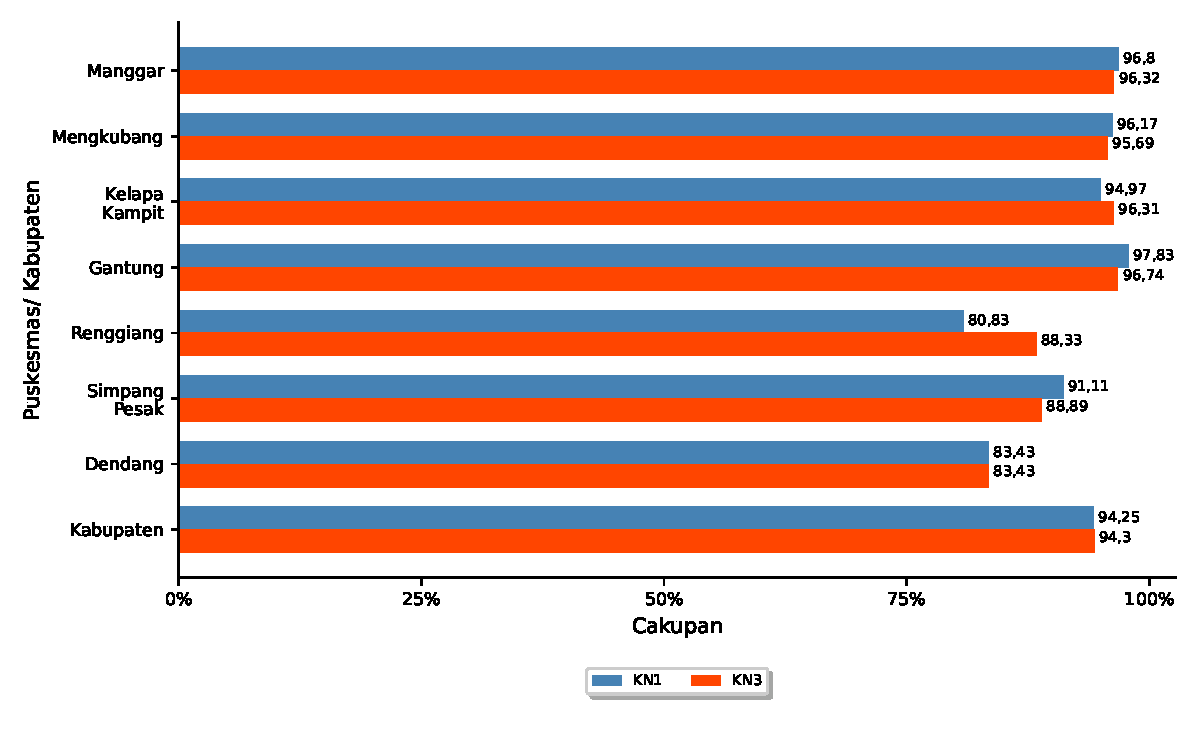
\includegraphics[width=0.9\textwidth]{bab_05/bab_05_14_KN1KN3}
    \caption{Cakupan KN1 dan KN Lengkap di Kabupaten Belitung Timur tahun \tP per Puskesmas}
    \label{fig:Cakupan-KN1-KNlengkap}
\end{figure}

%\begin{figure}[H]
%    \centering
%%%    \includegraphics[width=0.9\textwidth]{bab_05/bab_05_14a_plotKN1KN3}
%    \caption{Cakupan KN1 dan KN Lengkap di Kab. Belitung Timur Tahun 2017-2021}
%    \label{fig:KN1-KNlengkap-2016-2020}
%\end{figure}

Hipotiroid Kongenital adalah gangguan defisiensi hormon tiroid yang timbul pada bayi baru lahir yang dapat menimbulkan gangguan tumbuh kembang pada bayi.
Skrining Hipotiroid Kongenital (SHK) dilakukan dengan mengambil spesimen darah pada tumit bayi baru lahir berusia minimal 48 sampai 72 jam dan maksimal 2 minggu.

Cakupan SHK di Kabupaten Belitung Timur pada tahun \tP adalah sebesar 72,42\%.

\begin{figure}[H]
	\centering
	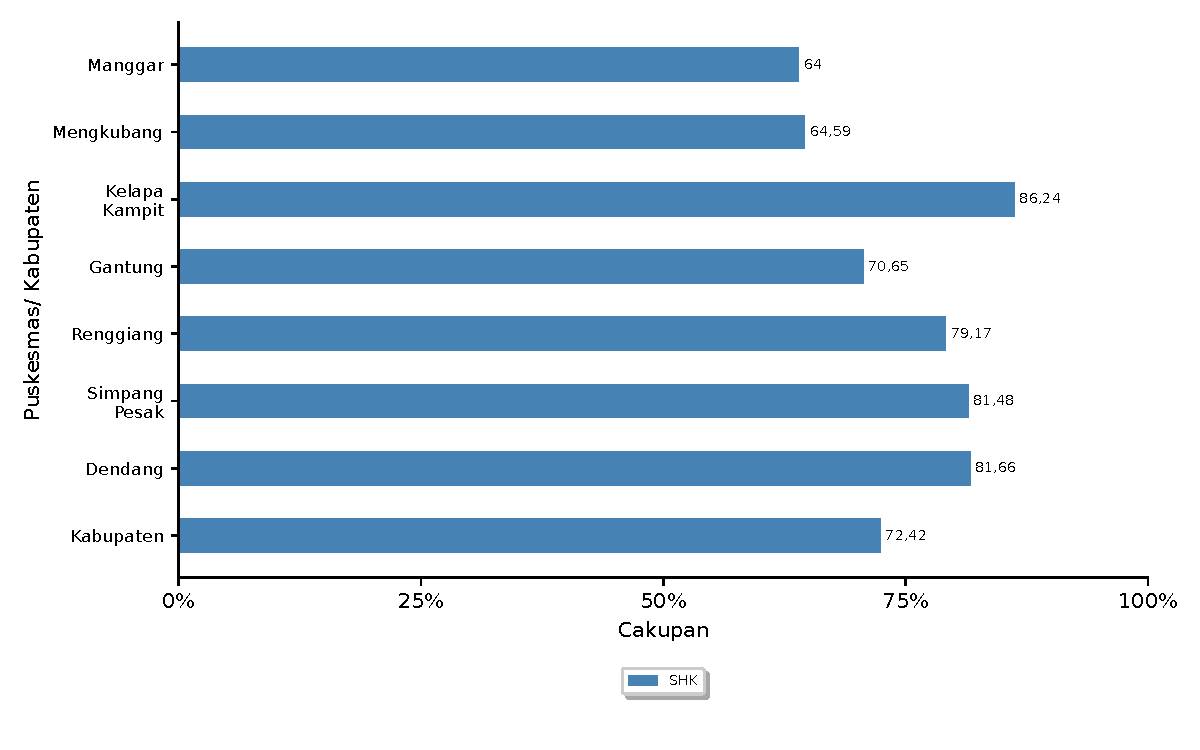
\includegraphics[width=0.9\textwidth]{bab_05/bab_05_14c_SHK}
	\caption{Cakupan SHK di Kabupaten Belitung Timur tahun \tP per Puskesmas}
	\label{fig:Cakupan-SHK}
\end{figure}

\subsection{Bayi Mendapat ASI Eksklusif}
Air Susu Ibu (ASI) adalah cairan hasil sekresi kelenjar payudara ibu
untuk konsumsi bayi dan merupakan sumber gizi utama bayi yang belum
dapat mencerna makanan padat. ASI eksklusif berdasarkan Peraturan
Pemerintah Nomor 33 Tahun 2012 adalah ASI yang diberikan kepada bayi
sejak dilahirkan selama enam bulan, tanpa menambahkan dan/atau mengganti
dengan makanan atau minuman lain (kecuali obat, vitamin, dan mineral).

Cakupan bayi mendapat ASI eksklusif di kabupaten Belitung Timur pada
tahun \tP yaitu sebesar 46,96\% (\autoref{fig:Cakupan-Bayi-ASI-Eksklusif}).
% meningkat dari cakupan tahun 2021 sebesar 45,62\%.

\begin{figure}[H]
  \centering
  \includegraphics[width=0.9\textwidth]{bab_05/bab_05_15_ASIeksklusif}
  \caption{Cakupan Bayi Mendapat ASI Eksklusif di Kab. Belitung Timur Tahun \tP per Puskesmas}
  \label{fig:Cakupan-Bayi-ASI-Eksklusif}
\end{figure}

\subsection{Pelayanan Kesehatan Bayi}
Pelayanan kesehatan bayi adalah pelayanan kesehatan pada bayi minimal
4 kali yaitu satu kali pada umur 29 hari-2 bulan, 1 kali pada umur
3-5 bulan, 1 kali pada umur 6-8 bulan, dan 1 kali pada umur 9-11 bulan.
Pelayanan Kesehatan tersebut meliputi pemberian imunisasi dasar (BCG,
DPT/HB1-3, Polio 1-4, Campak), pemantauan pertumbuhan, Stimulasi Deteksi
Intervensi Dini Tumbuh Kembang (SDIDTK), pemberian vitamin A pada
bayi umur 6-11 bulan, penyuluhan pemberian ASI eksklusif dan Makanan
Pendamping ASI (MP ASI).

Cakupan pelayanan kesehatan bayi di Kabupaten Belitung Timur pada
tahun \tP adalah sebesar 96,74\% (~\autoref{fig:Cakupan-Pelayanan-Kesehatan-Bayi}).
% meningkat dari cakupan tahun 2020 sebesar 94,11\%.

\begin{figure}[H]
    \centering
    \includegraphics[width=0.85\textwidth]{bab_05/bab_05_16_pelayananBayi}
    \caption{Cakupan Pelayanan Kesehatan Bayi di Kab. Belitung Timur tahun \tP per Puskesmas}
    \label{fig:Cakupan-Pelayanan-Kesehatan-Bayi}
\end{figure}

\subsection{Cakupan Desa/ Kelurahan UCI}
Pencapaian \emph{Universal Child Immunization} (UCI) pada dasarnya merupakan
\emph{proxy} terhadap cakupan sasaran bayi yang telah mendapatkan imunisasi
secara lengkap. Desa/ kelurahan UCI adalah Desa/ kelurahan dimana
paling sedikit 80\% dari jumlah bayi yang ada di desa tersebut sudah
mendapat imunisasi dasar lengkap dalam waktu satu tahun.

Pada tahun \tP sebanyak 35 desa dari total 39 desa yang ada di Kabupaten Belitung
Timur telah mencapai UCI, sehingga capaian UCI Kabupaten Belitung
Timur pada tahun \tP adalah 89,74\% (\autoref{fig:Cakupan-Desa-UCI}).

\begin{figure}[H]
    \centering
    \includegraphics[width=0.85\textwidth]{bab_05/bab_05_17_UCI}
    \caption{Cakupan Desa/ Kelurahan UCI di Kab. Belitung Timur Tahun \tP per Puskesmas}
    \label{fig:Cakupan-Desa-UCI}
\end{figure}

\subsection{Imunisasi}
Imunisasi adalah upaya stimulasi terhadap sistem kekebalan tubuh untuk
menghasilkan antibodi dalam upaya melawan penyakit menular tertentu.
Program imunisasi melalui pemberian vaksin merangsang antibodi menggunakan
antigen yang telah dilemahkan yang berasal dari vaksin. Beberapa penyakit
menular yang termasuk ke dalam Penyakit yang Dapat Dicegah dengan
Imunisasi (PD3I) antara lain TBC, Difteri, Tetanus, Hepatitis B, Pertusis,
Campak, Polio, radang selaput otak, dan radang paru-paru.

\subsubsection{Imunisasi pada bayi}
Imunisasi dasar bayi meliputi pemberian imunisasi Hepatitis B pada
bayi usia 0-7 hari, imunisasi BCG pada bayi usia 0-11 bulan, imunisasi
Polio pada bayi usia 0-11 bulan dengan interval minimal 1 bulan, imunisasi
DPT-HB/DPT-HB-Hib pada bayi usia 2-11 bulan dengan interval minimal
1 bulan, dan imunisasi Campak pada bayi usia 9-11 bulan.

Cakupan imunisasi HB0 di Kabupaten Belitung Timur pada tahun \tP adalah sebesar 94,54\% (\autoref{fig:Cakupan-Imunisasi-HB0}), dan cakupan imunisasi BCG adalah 88,54\% (\autoref{fig:Cakupan-Imunisasi-BCG}).

Cakupan imunisasi DPT-HB-Hib3 di Kabupaten Belitung Timur pada tahun \tP
adalah sebesar 87,09\% (\autoref{fig:Cakupan-Imunisasi-DPT}), dan cakupan imunisasi Polio 4 adalah 87,24\% (\autoref{fig:Cakupan-Imunisasi-Polio4}).

Program imunisasi pada bayi bertujuan agar setiap bayi mendapatkan
imunisasi dasar secara lengkap. Bayi dikatakan mendapat imunisasi
dasar lengkap jika telah menerima 1 dosis imunisasi Hepatitis B, 1
dosis imunisasi BCG, 3 dosis imunisasi DPT-HB/DPT-HB-Hib, 4 dosis
imunisasi polio, dan 1 dosis imunisasi campak.

\begin{figure}[H]
    \centering
    \includegraphics[width=0.85\textwidth]{bab_05/bab_05_18a_imunHB0}
    \caption{Cakupan Imunisasi HB0 di Kab. Belitung Timur Tahun \tP per Puskesmas}
    \label{fig:Cakupan-Imunisasi-HB0}
\end{figure}

\begin{figure}[H]
    \centering
    \includegraphics[width=0.85\textwidth]{bab_05/bab_05_18b_imunBCG}
    \caption{Cakupan Imunisasi BCG di Kab. Belitung Timur Tahun \tP per Puskesmas}
    \label{fig:Cakupan-Imunisasi-BCG}
\end{figure}

\begin{figure}[H]
    \centering
    \includegraphics[width=0.85\textwidth]{bab_05/bab_05_19a_imunDPT}
    \caption{Cakupan Imunisasi DPT-HB-Hib3 di Kab. Belitung Timur Tahun \tP per Puskesmas}
    \label{fig:Cakupan-Imunisasi-DPT}
\end{figure}

\begin{figure}[H]
    \centering
    \includegraphics[width=0.85\textwidth]{bab_05/bab_05_19b_imunPol4}
    \caption{Cakupan Imunisasi Polio 4 di Kab. Belitung Timur Tahun \tP per Puskesmas}
    \label{fig:Cakupan-Imunisasi-Polio4}
\end{figure}

\begin{figure}[H]
    \centering
    \includegraphics[width=0.85\textwidth]{bab_05/bab_05_20a_imunCampak}
    \caption{Cakupan Imunisasi Campak di Kab. Belitung Timur Tahun \tP per Puskesmas}
    \label{fig:Cakupan-Imunisasi-Campak}
\end{figure}

Cakupan imunisasi Campak di Kabupaten Belitung Timur pada tahun \tP adalah sebesar 91,71\% (\autoref{fig:Cakupan-Imunisasi-Campak}).
%menurun dari cakupan tahun 2019 sebesar 92,03\%.

Cakupan imunisasi dasar lengkap (IDL) di Kabupaten Belitung Timur pada tahun \tP adalah sebesar 92,77\% (\autoref{fig:Cakupan-Imunisasi-IDL}).

\begin{figure}[H]
    \centering
    \includegraphics[width=0.85\textwidth]{bab_05/bab_05_20b_imunIDL}
    \caption{Cakupan Imunisasi Dasar Lengkap di Kab. Belitung Timur Tahun \tP per Puskesmas}
    \label{fig:Cakupan-Imunisasi-IDL}
\end{figure}

\subsubsection{Imunisasi pada balita}
Imunisasi lanjutan diperlukan untuk mempertahankan tingkat kekebalan yang optimal pada anak.
Imunisasi lanjutan meliputi pemberian imunisasi DPT-HB-Hib 4 pada anak usia 12-24 bulan serta imunisasi Campak 2 pada anak usia 12-24 bulan.

Cakupan imunisasi DPT-HB-Hib 4 di Kabupaten Belitung Timur pada tahun \tP
adalah sebesar 72,79\% (\autoref{fig:Cakupan-Imunisasi-DPT4}), sedangkan cakupan imunisasi Campak 2 adalah 73,34\% (\autoref{fig:Cakupan-Imunisasi-Campak2}).

\begin{figure}[H]
    \centering
    \includegraphics[width=0.85\textwidth]{bab_05/bab_05_21a_imunDPTlanjut}
    \caption{Cakupan Imunisasi DPT-HB-Hib 4 di Kab. Belitung Timur Tahun \tP per Puskesmas}
    \label{fig:Cakupan-Imunisasi-DPT4}
\end{figure}

\begin{figure}[H]
    \centering
    \includegraphics[width=0.85\textwidth]{bab_05/bab_05_21b_imunCampakLanjut}
    \caption{Cakupan Imunisasi Campak 2 di Kab. Belitung Timur Tahun \tP per Puskesmas}
    \label{fig:Cakupan-Imunisasi-Campak2}
\end{figure}

\subsection{Pemberian Kapsul Vitamin A}
Upaya perbaikan gizi juga dilakukan kepada beberapa sasaran yang diperkirakan
banyak mengalami kekurangan Vitamin A. Vitamin A adalah salah satu
zat gizi penting yang larut dalam lemak, disimpan dalam hati, dan
tidak dapat diproduksi oleh tubuh sehingga harus dipenuhi dari luar
tubuh. Kekurangan Vitamin A (KVA) dapat menurunkan sistem kekebalan
tubuh balita serta meningkatkan risiko kesakitan dan kematian. Kekurangan
Vitamin A juga merupakan penyebab utama kebutaan pada anak yang dapat
dicegah.

Pemberian Vitamin A dilakukan berupa pemberian kapsul vitamin A biru 100.000 IU bagi bayi
usia enam sampai dengan sebelas bulan, dan kapsul vitamin A merah 200.000
IU untuk anak balita usia dua belas sampai dengan lima puluh sembilan sebanyak
bulan.

Cakupan pemberian vitamin A pada balita usia 6-59 tahun pada tahun \tP di Kabupaten Belitung Timur adalah 86,60\% (\autoref{fig:Cakupan-Vitamin-A-Balita}).
% meningkat dari cakupan tahun 2021 sebesar 81,47\%.

\begin{figure}[H]
    \centering
    \includegraphics[width=0.9\textwidth]{bab_05/bab_05_22_bayiBalitaVitA}
    \caption{Cakupan Pemberian Vitamin A Balita 6-59 Bulan di Kab. Belitung Timur Tahun \tP per Puskesmas}
    \label{fig:Cakupan-Vitamin-A-Balita}
\end{figure}


\subsection{Pelayanan Kesehatan Anak Balita}
Pelayanan kesehatan anak balita mencakup pemantauan tumbuh kembang dan pelayanan Stimulasi Deteksi dan Intervensi Dini Tumbuh Kembang (SDIDTK).
Balita yang dipantau tumbuh kembang adalah  balita yang ditimbang sedikitnya 8 kali dalam satu tahun, diukur panjang badan atau tinggi badannya sedikitnya 2 kali dalam satu tahun dan dipantau perkembangan sedikitnya 2 kali dalam satutahun. Pemantauan perkembangan menggunakan ceklis Buku KIA atau KPSP atau instrument baku lainnya.
Balita dilayani SDIDTK adalah balita yang dipantau tahapan perkembangan sesuai usianya (usia 0-24 bulan: 3 bulan sekali; usia 24-72 bulan: 6 bulan sekali) menggunakan instrument dalam SDIDTK oleh tenaga kesehatan dalam kurun waktu 1 tahun.

Cakupan balita dipantau tumbuh kembang di Kabupaten Belitung Timur pada tahun \tP adalah sebesar 99,01\%, sedangkan cakupan balita dilayani SDIDTK di Kabupaten Belitung Timur pada tahun \tP adalah sebesar 82,52\%. (\autoref{fig:Cakupan-Pelayanan-Balita-Tumbuh-Kembang}).

\begin{figure}[H]
	\centering
	\includegraphics[width=0.85\textwidth]{bab_05/bab_05_23_balitaTumbuhKembang}
	\caption{Cakupan Balita Dipantau Tumbuh Kembang di Kab. Belitung Timur tahun \tP per Puskesmas}
	\label{fig:Cakupan-Pelayanan-Balita-Tumbuh-Kembang}
\end{figure}

\subsection{Balita Ditimbang}
\label{subsec:Balita-Ditimbang}
Peran serta masyarakat dalam penimbangan balita menjadi sangat penting
dalam deteksi dini kasus gizi kurang dan gizi buruk. Dengan rajin
menimbang balita, maka pertumbuhan balita dapat dipantau secara intensif.
Sehingga bila berat badan anak tidak naik ataupun jika ditemukan penyakit
akan dapat segera dilakukan upaya pemulihan dan pencegahan supaya
tidak menjadi gizi kurang atau gizi buruk. Semakin cepat ditemukan,
maka penanganan kasus gizi kurang atau gizi buruk akan semakin baik.\par

Cakupan penimbangan balita di posyandu (D/S) adalah jumlah balita
yang ditimbang di seluruh posyandu yang melapor di satu wilayah kerja
pada kurun waktu tertentu dibagi jumlah seluruh balita yang ada di
seluruh posyandu yang melapor di satu wilayah kerja pada kurun waktu
tertentu.

Cakupan balita ditimbang di Kabupaten Belitung Timur pada tahun \tP yaitu sebesar 43,92\% (\autoref{fig:Cakupan-Balita-Ditimbang}), %meningkat dari cakupan tahun 2020 sebesar 57,91\%.

\begin{figure}[H]
  \centering
  \includegraphics[width=0.85\textwidth]{bab_05/bab_05_24_balitaDitimbang}
  \caption{Cakupan Balita Ditimbang di Kab. Belitung Timur Tahun \tP per Puskesmas}
  \label{fig:Cakupan-Balita-Ditimbang}
\end{figure}


\subsection{Penemuan Kasus Balita Gizi Kurang, Balita Pendek, dan Balita Kurus}
\label{subsec:Penemuan-Kasus-Gizi-Kurang}
Balita Berat Badan Kurang adalah balita dengan status gizi yang didasarkan pada indeks berat badan menurut umur (BB/U) yang merupakan gabungan dari istilah gizi buruk dan gizi kurang dengan Z score < -2 standar deviasi, di mana Z score adalah nilai simpangan berat badan atau tinggi badan dari nilai berat badan atau tinggi badan normal menurut baku pertumbuhan WHO.
Balita Pendek adalah balita dengan status gizi yang didasarkan pada indeks panjang badan menurut umur (PB/U) atau tinggi badan menurut umur (TB/U) dengan Z score < -2 standar deviasi.
Balita Gizi Kurang adalah balita dengan status gizi yang didasarkan pada indeks berat badan menurut panjang badan (BB/PB) atau berat badan menurut tinggi badan (BB/TB) dengan Z score -2 hingga -3 standar deviasi.
Balita Gizi Buruk adalah balita dengan status gizi yang didasarkan pada indeks berat badan menurut panjang badan (BB/PB) atau berat badan menurut tinggi badan (BB/TB) dengan Z score < -3 standar deviasi.

\begin{figure}[H]
  \centering
  \includegraphics[width=0.85\textwidth]{bab_05/bab_05_25_statusGiziBalita}
  \caption{Sebaran Status Gizi Balita Berdasarkan Indeks BB/U, TB/U, dan BB/TB di Kab. Belitung Timur Tahun \tP per
Puskesmas}
  \label{fig:Status-Gizi-Balita}
\end{figure}

Pada tahun \tP, tercatat bahwa kasus Balita Berat Badan Kurang (BB/U) berjumlah 618 kasus atau 8,57\% dari jumlah balita ditimbang.
Kasus Balita Pendek (TB/U) atau \textit{stunting} berjumlah 360 kasus atau 5,00\% dari jumlah balita ditimbang.
Kasus Balita Gizi Kurang (BB/TB) berjumlah 256 kasus atau 3,57 \% dari jumlah balita ditimbang.
Kasus Balita Gizi Buruk (BB/TB) berjumlah 3 kasus atau 0,04 \% dari jumlah balita ditimbang (\autoref{fig:Status-Gizi-Balita}).

\subsection{Penjaringan Kesehatan Siswa SD, SMP, SMA}
Penjaringan kesehatan siswa SD/ MI adalah pemeriksaan kesehatan umum terhadap murid kelas 1 SD, MI atau setingkat yang dilaksanakan oleh tenaga kesehatan bersama kader kesehatan sekolah yang mencakup minimal pemeriksaan status gizi (TB,BB), pemeriksaan gigi, tajam penglihatan dan tajam pendengaran di satu wilayah kerja pada kurun waktu tertentu.

Cakupan penjaringan kesehatan siswa SD/ MI di Kabupaten Belitung Timur pada tahun \tP adalah sebesar 100,00\%.

Penjaringan kesehatan siswa SMP dan setingkat adalah pemeriksaan kesehatan umum terhadap murid kelas 7 SMP, MTs atau setingkat yang dilaksanakan oleh tenaga kesehatan bersama kader kesehatan sekolah yang mencakup minimal pemeriksaan status gizi (TB,BB), pemeriksaan gigi, tajam penglihatan dan tajam pendengaran di satu wilayah kerja pada kurun waktu tertentu.

Cakupan penjaringan kesehatan siswa SMP/ MTs di Kabupaten Belitung Timur pada tahun \tP adalah sebesar 100,00\%.

Penjaringan kesehatan siswa SMA/ MA adalah pemeriksaan kesehatan umum terhadap murid kelas 10 SMA, MA atau setingkat yang dilaksanakan oleh tenaga kesehatan bersama kader kesehatan sekolah yang mencakup minimal pemeriksaan status gizi (TB,BB), pemeriksaan gigi, tajam penglihatan dan tajam pendengaran di satu wilayah kerja pada kurun waktu tertentu.

Cakupan penjaringan kesehatan siswa SMA/ MA di Kabupaten Belitung Timur pada tahun \tP adalah sebesar 100,00\%.

\begin{figure}[H]
    \centering
    \includegraphics[width=0.85\textwidth]{bab_05/bab_05_26_kesehatanSiswa}
    \caption{Cakupan Penjaringan Kesehatan Siswa SD/ MI, SMP/ MTs, SMA/ MA di Kab. Belitung Timur Tahun \tP per Kecamatan}
    \label{fig:Cakupan-Penjaringan-Siswa}
\end{figure}

Pelayanan kesehatan usia pendidikan dasar sesuai standar meliputi :
\begin{enumerate}
    \item Skrining kesehatan.
    \item Tindaklanjut hasil skrining kesehatan.
\end{enumerate}
yang dilakukan pada anak kelas 1 sampai dengan kelas 9 di sekolah minimal satu kali dalam satu tahun ajaran dan usia 7 sampai 15 tahun diluar sekolah.

Cakupan pelayanan kesehatan usia pendidikan dasar di Kabupaten Belitung Timur pada tahun \tP adalah sebesar 99,96\% (\autoref{fig:Cakupan-Pelayanan-Kesehatan-Usia-Dikdas}).

\begin{figure}[H]
    \centering
    \includegraphics[width=0.85\textwidth]{bab_05/bab_05_26_kesehatanSiswa_spm}
    \caption{Cakupan Pelayanan Kesehatan Usia Pendidikan Dasar di Kab. Belitung Timur Tahun \tP per Kecamatan}
    \label{fig:Cakupan-Pelayanan-Kesehatan-Usia-Dikdas}
\end{figure}

\section{KESEHATAN GIGI DAN MULUT}
\subsection{Pelayanan Kesehatan Gigi dan Mulut}
\todo{data not valid yet}
Setiap penyelenggaraan upaya kesehatan gigi dan mulut yang dilakukan untuk meningkatkan kesehatan gigi dan mulut, mencegah dan menyembuhkan penyakit serta memulihkan kesehatan gigi dan mulut perorangan, keluarga, kelompok atau masyarakat secara paripurna, terpadu dan berkualitas.
Pelayanan kesehatan gigi dan mulut yang diberikan dapat berupa pemeriksaan, pengobatan, pencabutan gigi tetap/gigi sulung, penambalan tetap/sementara, perawatan pulpa, pembersihan karang gigi dan pembuatan gigi tiruan lepasan.

Rasio tumpatan/pencabutan adalah rasio jumlah penambalan gigi tetap terhadap jumlah pencabutan gigi tetap dalam setahun.
Cakupan kasus gigi dan mulut dirujuk adalah persentase kasus gigi dan mulut yang dikirim dari Puskesmas ke fasilitas kesehatan rujukan tingkat lanjut dalam satu tahun terhadap jumlah kunjungan baru dan lama rawat jalan gigi dan mulut di puskesmas meliputi pemeriksaan, pengobatan dan perawatan gigi dan mulut dalam satu tahun.

Rasio tumpatan/pencabutan di Kabupaten Belitung Timur pada tahun \tP adalah sebesar 0,99 (\autoref{fig:Cakupan-Pelayanan-Kesehatan-Gigi-Mulut-Tumpatan}).

\begin{figure}[H]
	\centering
	%    \includegraphics[width=0.85\textwidth]{bab_05/bab_05_27a_gimulTumpatan}
	\caption{Rasio Tumpatan/Pencabutan di Kab. Belitung Timur Tahun \tP per Puskesmas}
	\label{fig:Cakupan-Pelayanan-Kesehatan-Gigi-Mulut-Tumpatan}
\end{figure}

Cakupan kasus gigi dan mulut dirujuk di Kabupaten Belitung Timur pada tahun \tP adalah sebesar 6,51\% (\autoref{fig:Cakupan-Pelayanan-Kesehatan-Gigi-Mulut-Dirujuk}).

\begin{figure}[H]
	\centering
%    \includegraphics[width=0.85\textwidth]{bab_05/bab_05_27b_gimulDirujuk}
	\caption{Cakupan Kasus Gigi dan Mulut Dirujuk di Kab. Belitung Timur Tahun \tP per Puskesmas}
	\label{fig:Cakupan-Pelayanan-Kesehatan-Gigi-Mulut-Dirujuk}
\end{figure}

\subsection{Upaya Kesehatan Gigi Sekolah}
Penyelenggaraan upaya kesehatan gigi dan mulut anak sekolah tingkat dasar (SD/MI) atau UKGS dilakukan dengan mengutamakan pendekatan promotif dan preventif tanpa mengabaikan pendekatan kuratif dan rehabilitatif.
Perawatan kesehatan gigi dan mulut diberikan kepada murid SD/MI dalam bentuk preventif (\textit{topical fluoride}, \textit{surface protection}/\textit{fissure sealent} atau \textit{atraumatic restoration treatment}) dan kuratif sederhana seperti pengobatan, penambalan gigi, dan pencabutan gigi sulung maupun tetap yang dilakukan baik di sekolah maupun Puskesmas.

Cakupan pemeriksaan gigi dan mulut pada murid SD/MI di Kabupaten Belitung Timur pada tahun \tP adalah sebesar 100,00\% (\autoref{fig:Cakupan-Pelayanan-Kesehatan-Gigi-Mulut-SD}).

\begin{figure}[H]
	\centering
%	\includegraphics[width=0.85\textwidth]{bab_05/bab_05_27c_gimulSDdiperiksa}
	\caption{Cakupan Pemeriksaan Gigi dan Mulut Murid SD/MI di Kab. Belitung Timur Tahun \tP per Puskesmas}
	\label{fig:Cakupan-Pelayanan-Kesehatan-Gigi-Mulut-SD}
\end{figure}

Cakupan perawatan gigi dan mulut pada murid SD/MI di Kabupaten Belitung Timur pada tahun \tP adalah sebesar 18,66\% (\autoref{fig:Cakupan-Pelayanan-Kesehatan-Gigi-Mulut-SD-Dirawat}).

\begin{figure}[H]
	\centering
%	\includegraphics[width=0.85\textwidth]{bab_05/bab_05_27d_gimulSDdirawat}
	\caption{Cakupan Perawatan Gigi dan Mulut Murid SD/MI di Kab. Belitung Timur Tahun \tP per Puskesmas}
	\label{fig:Cakupan-Pelayanan-Kesehatan-Gigi-Mulut-SD-Dirawat}
\end{figure}

\section[USIPRO DAN USILA]{KESEHATAN USIA PRODUKTIF DAN USIA LANJUT}
\subsection{Pelayanan Kesehatan Usia Produktif}
Cakupan pelayanan kesehatan usia produktif adalah cakupan penduduk usia 15–59 tahun yang mendapat pelayanan skrining kesehatan sesuai standar di wilayah kerjanya dalam kurun waktu satu tahun. Edukasi dilaksanakan di Fasilitas Pelayanan Kesehatan dan/ atau UKBM dan/ atau kunjungan rumah. Pelayanan kesehatan sesuai standar meliputi:
\begin{enumerate}
  \item Edukasi kesehatan termasuk keluarga berencana;
  \item Skrining faktor risiko penyakit menular dan penyakit tidak menular:
  \begin{enumerate}
    \item Pengukuran tinggi badan, berat badan, dan lingkar perut;
    \item Pengukuran tekanan darah;
    \item Pemeriksaan gula darah; dan
    \item Anamnesa perilaku berisiko.
  \end{enumerate}
\end{enumerate}

Cakupan pelayanan kesehatan usia produktif di Kabupaten Belitung Timur pada tahun \tP adalah 88,49\% (\autoref{fig:Cakupan-Yankes-Usprod}).
%, meningkat dari cakupan tahun 2021 sebesar 65,23\%.
Dari 74.911 orang penduduk yang diskrining, sebanyak 15.166 orang (20,25\%) ditemukan beresiko PTM (\autoref{fig:Cakupan-Resiko-PTM-Usprod}).

\begin{figure}[H]
    \centering
    \includegraphics[width=0.85\textwidth]{bab_05/bab_05_28_skriningProduktif_a}
    \caption{Cakupan Pelayanan Kesehatan Usia Produktif di Kab. Belitung Timur Tahun \tP per Puskesmas}
    \label{fig:Cakupan-Yankes-Usprod}
\end{figure}

\begin{figure}[H]
    \centering
    \includegraphics[width=0.85\textwidth]{bab_05/bab_05_28_skriningProduktif_b}
    \caption{Penemuan Resiko PTM Usia Produktif di Kab. Belitung Timur Tahun \tP per Puskesmas}
    \label{fig:Cakupan-Resiko-PTM-Usprod}
\end{figure}

\subsection{Pelayanan Kesehatan Calon Pengantin}
Calon pengantin (catin) merupakan kelompok sasasan yang perlu mendapatkan intervensi dalam pelayanan kesehatan reproduksi.
Pemberian KIE kesehatan reproduksi kepada calon pengantin merupakan salah satu upaya strategis untuk meningkatkan derajat kesehatan ibu dan bayi baru lahir melalui peningkatan pengetahuan calon pengantin agar kelak dapat merencanakan kehamilan yang sehat dan melahirkan generasi penerus yang berkualitas.

Cakupan pelayanan kesehatan calon pengantin di Kabupaten Belitung Timur pada tahun \tP adalah 97,84\% (\autoref{fig:Cakupan-Yankes-Catin}).

\begin{figure}[H]
	\centering
	\includegraphics[width=0.85\textwidth]{bab_05/bab_05_29a_pelayananCatin}
	\caption{Cakupan Pelayanan Kesehatan Calon Pengantin di Kab. Belitung Timur Tahun \tP per Puskesmas}
	\label{fig:Cakupan-Yankes-Catin}
\end{figure}

Dari 905 catin perempuan yang diperiksa ditemukan 209 orang (23,09\%) yang mengidap anemia dan 157 orang (17,35\%) yang mengalami gizi kurang.

\begin{figure}[H]
	\centering
	\includegraphics[width=0.85\textwidth]{bab_05/bab_05_29b_catinResiko}
	\caption{Penemuan Catin Perempuan Anemia dan Gizi Kurang di Kab. Belitung Timur Tahun \tP per Puskesmas}
	\label{fig:Cakupan-Yankes-Catin-Anemia}
\end{figure}

\subsection{Pelayanan Kesehatan Usia Lanjut}
Cakupan pelayanan kesehatan usia lanjut adalah pelayanan kesehatan untuk warga negara usia 60 tahun ke atas dalam bentuk edukasi dan skrining usia
lanjut sesuai standar pada satu wilayah kerja dalam kurun waktu satu tahun. Edukasi dilaksanakan di Fasilitas Pelayanan Kesehatan dan/atau UKBM dan/atau kunjungan rumah. Komponen skrining kesehatan yang dilakukan pada usia lanjut terdiri dari:
\begin{enumerate}
  \item Pengukuran tinggi badan, berat badan, dan lingkar perut;
  \item Pengukuran tekanan darah;
  \item Pemeriksaan gula darah;
  \item Pemeriksaan gangguan mental;
  \item Pemeriksaan gangguan kognitif;
  \item Pemeriksaan tingkat kemandirian usia lanjut; dan
  \item Anamnesa perilaku berisiko.
\end{enumerate}

Cakupan pelayanan kesehatan usia lanjut di Kabupaten Belitung Timur pada tahun \tP adalah 87,07\% (\autoref{fig:Cakupan-Yankes-Usila}).
% menurun dari cakupan tahun 2021 sebesar 69,55\%.

\begin{figure}[H]
    \centering
    \includegraphics[width=0.85\textwidth]{bab_05/bab_05_30_skriningLansia}
    \caption{Cakupan Pelayanan Kesehatan Usia Lanjut di Kab. Belitung
Timur Tahun \tP per Puskesmas}
    \label{fig:Cakupan-Yankes-Usila}
\end{figure}

\clearpage
% \chapter{PENGENDALIAN PENYAKIT}
Pengendalian penyakit sebagai upaya penurunan insiden, prevalensi, morbiditas atau mortalitas dari suatu penyakit, mempunyai peranan penting untuk mengukur derajat kesehatan masyarakat. Pengendalian penyakit menular meliputi penyakit menular langsung, penyakit yang dapat dikendalikan dengan imunisasi dan penyakit yang ditularkan melalui binatang. Sedangkan pengendalian penyakit tidak menular meliputi upaya pencegahan dan deteksi dini penyakit tidak menular tertentu.

\section{PENYAKIT TERBANYAK}
Peringkat pertama penyakit terbanyak di Kabupaten Belitung Timur pada Tahun \tP yang tercatat di keseluruhan Puskesmas adalah Penyakit Tekanan Darah Tinggi/ Hipertensi primer, sebanyak 8.956 kasus (\autoref{fig:10-penyakit-terbanyak}).
Sedangkan peringkat ke-sepuluh adalah Non-insulin-dependent diabetes
mellitus, sebanyak 511 kasus.

\begin{figure}[H]
    \centering
    \includegraphics[width=\textwidth]{bab_06/bab_06_00_penyakitTerbanyak}
    \caption{Jumlah 10 Penyakit Terbanyak di Kab. Belitung Timur Tahun \tP}
    \label{fig:10-penyakit-terbanyak}
\end{figure}

\section[PENGENDALIAN PM]{PENGENDALIAN PENYAKIT MENULAR LANGSUNG}
Pengendalian penyakit menular lebih ditekankan pada pelaksanaan surveilans dan epidemologi dengan upaya penemuan penderita secara dini yang ditindaklanjuti dengan penanganan secara cepat. Di samping itu pelayanan lain yang diberikan adalah pemberian imunisasi, upaya penanggulangan faktor resiko melalui program peningkatan kualitas lingkungan serta peningkatan peran serta masyarakat dalam upaya pemberantasan penyakit menular yang dilaksanakan dengan berbagai bentuk kegiatan.

\subsection{Penyakit TB Paru}
Tuberkulosis (TB) Paru merupakan penyakit menular langsung yang disebabkan oleh infeksi bakteri \emph{Mycobacterium tuberculosis} yang menyerang jaringan paru. Gejala utama yaitu batuk berdahak selama 2-3 minggu atau lebih.

\emph{Treatment Coverage} TBC adalah jumlah semua kasus tuberkulosis yang ditemukan dan diobati di antara perkiraan jumlah semua kasus tuberkulosis (insiden
tuberkulosis). Pada tahun \tP terdapat 266 kasus TB di Kabupaten Belitung Timur (\autoref{fig:Jumlah-Kasus-TB}) sehingga TC TB pada tahun \tP adalah sebesar 44,28\%.

\begin{figure}[H]
  \centering
  \includegraphics[width=0.85\textwidth]{bab_06/bab_06_01a_kasusTB}
  \caption{Jumlah Kasus TB di Kab. Belitung Timur Tahun \tP per Puskesmas}
  \label{fig:Jumlah-Kasus-TB}
\end{figure}

Cakupan penemuan TB anak adalah jumlah seluruh kasus tuberkulosis anak yang ditemukan di antara perkiraan jumlah kasus tuberkulosis anak yang ada disuatu wilayah dalam periode tertentu. Perkiraan jumlah kasus tuberkulosis  anak adalah 12\% dari perkiraan jumlah semua kasus TB (insiden) yang ada di masing-masing kabupaten/ kota. Jumlah kasus TB anak pada tahun \tP adalah sebanyak 54 kasus, sehingga cakupan penemuan TB anak adalah sebesar 72,35\%.

\begin{figure}[H]
    \centering
    \includegraphics[width=0.85\textwidth]{bab_06/bab_06_01b_cureCompSuccRateTB}
    \caption{\emph{Cure Rate} \& \emph{Success Rate} TB paru di Kab. Belitung Timur Tahun \tP per Puskesmas}
    \label{fig:Cure-Rate-TB}
\end{figure}

Upaya pencegahan dan pemberantasan TB-Paru dilakukan dengan pendekatan
DOTS (\emph{Directly Observe Treatment Shortcourse}) atau pengobatan TB-Paru
dengan pengawasan langsung oleh Pengawas Menelan Obat (PMO). Kegiatan
ini berupaya menemukan penderita dengan pemeriksaan dahak di sarana
pelayanan kesehatan yang ditindaklanjuti dengan paket pengobatan.

Angka Kesembuhan (\emph{Cure Rate}) TB paru terkonfirmasi biologis adalah jumlah pasien TB paru terkonfirmasi biologis yang sembuh di suatu wilayah pada kohort yang sama dengan hasil pemeriksaan bakteriologis pada akhir pengobatan menjadi negatif dan pada salah satu pemeriksaan sebelumnya.
\emph{Cure Rate} pada tahun \tP di Kabupaten Belitung Timur adalah sebanyak 48 orang (52,75\%).

Angka Pengobatan Lengkap (\emph{Complete Rate}) TB adalah jumlan pasien tuberkulosis yang telah menyelesaikan pengobatan secara lengkap dimana pada salah satu pemeriksaan sebelum akhir pengobatan hasilnya negatif namun tanpa ada bukti hasil pemeriksaan bakteriologis pada akhir pengobatan.
\emph{Complete Rate} pada tahun \tP di Kabupaten Belitung Timur adalah sebanyak 32 orang (35,16\%).

Angka Keberhasilan Pengobatan (\emph{Success Rate}) TBadalah jumlah pasien tuberkulosis semua kasus yang sembuh dan pengobatan lengkap diantara semua kasus tuberkulosis yang diobati dan dilaporkan.
\emph{Success Rate} pada tahun \tP di Kabupaten Belitung Timur adalah sebanyak 80 orang (87,91\%).

Terdapat 6 kasus kematian akibat TB di Kabupaten Belitung Timur pada tahun \tPnos atau 6,59\% dari jumlah kasus.

\begin{figure}[H]
	\centering
	\includegraphics[width=0.85\textwidth]{bab_06/bab_06_01c_kematianTB}
	\caption{Kematian pada pengobatan TB paru di Kab. Belitung Timur Tahun \tP per Puskesmas}
	\label{fig:kematian-TB}
\end{figure}

\subsection{Penyakit Pneumonia}
Pneumonia balita adalah balita mengalami batuk dan atau kesukaran bernapas dan hasil perhitungan napas, usia 0-2 bulan $\geq$60 kali/menit, usia 2-12 bulan $\geq$ 50 kali/menit, usia 12-59 bulan $\geq$ 40 kali/menit. Pneumonia berat jika balita mengalami tarikan dinding dada ke dalam (TDDK) atau saturasi oksigen $<$ 90.\

Tatalaksana pneumonia sesuai standar adalah jika balita dengan keluhan batuk dan atau kesukaran bernafas yang berkunjung ke sarana kesehatan diberikan tatalaksana standar dilakukan hitung napas/ melihat TDDK. Cakupan tatalaksana pneumonia sesuai standar di Kabupaten Belitung Timur pada tahun \tP adalah sebesar 99,79\% (\autoref{fig:Penemuan-Pneumonia-Balita}).

Penemuan penderita pneumonia balita adalah cakupan balita dengan pneumonia yang ditemukan dan diberikan tatalaksana sesuai standar di sarana kesehatan di satu wilayah dalam waktu satu tahun. Penemuan kasus penumonia balita di Kabupaten Belitung Timur pada tahun \tP adalah sebesar 10,92\% dari target penemuan.

\begin{figure}[H]
    \centering
    \includegraphics[width=0.9\textwidth]{bab_06/bab_06_02_pneumoniaBalita}
    \caption{Cakupan Penanganan dan Penemuan Pneumonia Pada Balita di Kab. Belitung Timur Tahun \tP per Puskesmas}
    \label{fig:Penemuan-Pneumonia-Balita}
\end{figure}


\subsection{Penyakit HIV/ AIDS}
HIV/ AIDS merupakan penyakit menular yang disebabkan oleh infeksi
\emph{Human Immunodeficiency Virus} yang menyerang sistem kekebalan tubuh.
Infeksi tersebut menyebabkan penderita mengalami penurunan ketahanan
tubuh sehingga sangat mudah untuk terinfeksi berbagai macam penyakit
lain.

Pelayanan kesehatan yang diberikan kepada orang dengan risiko terinfeksi virus HIV meliputi: pemberian komunikasi, informasi, dan edukasi (KIE) tentang HIV termasuk promosi kesehatan penggunaan alat pencegahan yang efektif (kondom, lubrikan (pelumas), alat suntik steril, dll); pelayanan pemeriksaan laboratorium berupa skrining (deteksi dini) HIV, dan pelayanan konfirmasi diagnosis rujukan ke layanan pengobatan Anti Retroviral (ARV). Sedangkan yang termasuk orang dengan resiko terinfeksi HIV adalah:
\begin{enumerate}
  \item Ibu hamil;
  \item Pasien TBC;
  \item Pasien Infeksi Menular Seksual (IMS);
  \item Penjaja seks;
  \item Lelaki yang berhubungan seks dengan lelaki (LSL);
  \item Transgender/Waria;
  \item Pengguna napza suntik (penasun);
  \item Warga Binaan Pemasyarakatan; dan
  \item Kelompok rentan.
\end{enumerate}

Jumlah Kasus HIV di Kabupaten Belitung Timur tahun \tP adalah sebanyak 0 kasus (\autoref{fig:Jumlah-Kasus-HIV}), sedangkan cakupan pelayanan deteksi dini HIV di Kabupaten Belitung Timur pada tahun \tP adalah sebesar 93,81\%.

\begin{figure}[H]
  \centering
  \includegraphics[width=0.85\textwidth]{bab_06/bab_06_03a_HIV}
  \caption{Jumlah Kasus HIV Kab. Belitung Timur Tahun \tP}
  \label{fig:Jumlah-Kasus-HIV}
\end{figure}

Antiretroviral (ARV) merupakan bagian dari pengobatan HIV dan AIDS untuk mengurangi risiko penularan HIV, menghambat perburukan infeksi oportunistik, meningkatkan kualitas hidup penderita HIV, dan menurunkan jumlah virus (\emph{viral load}) dalam darah sampai tidak terdeteksi. Cakupan orang dengan HIV (ODHIV) baru yang mendapat pengobatan ARV di Kabupaten Belitung Timur pada tahun \tP adalah sebesar 73,08\%.

\begin{figure}[H]
  \centering
  \includegraphics[width=0.85\textwidth]{bab_06/bab_06_03b_ARV}
  \caption{ODHIV ARV Kab. Belitung Timur Tahun \tP}
  \label{fig:HIV-ARV}
\end{figure}

Upaya pelayanan kesehatan dalam rangka penanggulangan HIV/AIDS di samping ditujukan pada penanganan penderita yang ditemukan juga diupayakan pada pencegahan melalui penemuan penderita secara dini yang dilanjutkan dengan konseling.
Kegiatan yang telah dilaksanakan di Kabupaten Belitung Timur tahun \tP dalam rangka penurunan angka kesakitan akibat HIV/AIDS dan PMS antara lain adalah Penyebaran Informasi (KIE) HIV/AIDS, Sero Survei HIV/AIDS, Skrining Darah, serta Monitoring dan Evaluasi HIV/AIDS.

\subsection{Penyakit Diare}
Diare adalah suatu penyakit yang ditandai dengan perubahan bentuk dan konsistensi tinja yang lembek sampai mencair dan bertambahnya frekuensi buang air besar yang lebih dari biasa, yaitu 3 kali atau lebih dalam sehari yang mungkin dapat disertai dengan muntah atau tinja yang berdarah.
Penyebab diare dikelompokkan dalam 6 golongan besar, yaitu infeksi (bakteri/ virus/ parasit), malabsorpsi, alergi, keracunan, imunodefisiensi dan sebab-sebab lainnya. Diare biasanya berlangsung beberapa hari, namun sebagian kasus dapat memanjang hingga beberapa minggu.
Diare dapat menyebabkan kematian; publikasi WHO pada tahun 2009 menunjukkan diare adalah penyebab kedua terbanyak kematian pada balita secara global.

Jumlah perkiraan kasus diare tahun \tP di Kabupaten Belitung Timur sebanyak 1.582 kasus balita dan 3.484 kasus semua umur.
Jumlah kasus yang ditemukan sebesar 304 kasus balita (19,22\%) dan 1.032 kasus semua umur (29,62\%) (\autoref{fig:Cakupan-Kasus-Diare-Dilayani}).

\begin{figure}[H]
    \centering{}
    \includegraphics[width=0.9\textwidth]{bab_06/bab_06_04a_diareDilayani}
    \caption{Cakupan Penanganan Kasus Diare di Kab. Belitung Timur Tahun \tP per Puskesmas}
    \label{fig:Cakupan-Kasus-Diare-Dilayani}
\end{figure}

\begin{figure}[H]
	\centering{}
	\includegraphics[width=0.9\textwidth]{bab_06/bab_06_04b_diareOralit}
	\caption{Cakupan Kasus Diare Diberi Oralit di Kab. Belitung Timur Tahun \tP per Puskesmas}
	\label{fig:Cakupan-Kasus-Diare-Oralit}
\end{figure}

\begin{figure}[H]
	\centering{}
	\includegraphics[width=0.9\textwidth]{bab_06/bab_06_04c_diareZinc}
	\caption{Cakupan Kasus Diare Diberi Zinc di Kab. Belitung Timur Tahun \tP per Puskesmas}
	\label{fig:Cakupan-Kasus-Diare-Zinc}
\end{figure}

\subsection{Deteksi Hepatitis B}
Hepatitis B adalah penyakit menular dalam bentuk peradangan hati yang disebabkan oleh virus Hepatitis B. Virus Hepatitis B menyebar melalui darah atau cairan tubuh. Di Indonesia, penularan Hepatitis B umumnya terjadi pada bayi pada saat proses kelahirannya. Deteksi dini Hepatitis B pada ibu hamil dapat membantu memitigasi penularan virus dari ibu ke bayi. Deteksi dini Hepatitis B dilakukan melalui pemeriksaan HBsAg. HBsAg (\emph{Hepatitis B Surface Antigen}) merupakan antigen permukaan yang ditemukan pada virus hepatitis B yang memberikan arti adanya infeksi hepatitis B.

Cakupan deteksi dini Hepatitis B pada ibu hamil di Kabupaten Belitung Timur pada tahun \tP adalah sebesar 83,33\% , dan ditemukan 2,33\% ibu hamil menunjukkan hasil reaktif.

\begin{figure}[H]
	\centering{}
	\includegraphics[width=0.9\textwidth]{bab_06/bab_06_05a_bumilHB}
	\caption{Cakupan Deteksi Hepatitis B pada Ibu Hamil di Kab. Belitung Timur Tahun \tP per Puskesmas}
	\label{fig:Cakupan-Bumil-HB}
\end{figure}

HBIg (\emph{Hepatitis B Immunoglubulin}) merupakan serum antibodi spesifik Hepatitis B yang memberikan perlindungan langsung kepada bayi yang lahir dari ibu dengan HBSAg reaktif (positif). HBIg efektif diberikan kepada bayi sebelum 24 jam setelah lahir.

Cakupan bayi lahir dari ibu yang reaktif HBsAg mendapat HBIG di Kabupaten Belitung Timur pada tahun \tP adalah sebesar 100\% .

\begin{figure}[H]
	\centering{}
	\includegraphics[width=0.9\textwidth]{bab_06/bab_06_05b_bayiHBIG}
	\caption{Cakupan Deteksi Hepatitis B pada Bayi di Kab. Belitung Timur Tahun \tP per Puskesmas}
	\label{fig:Cakupan-Bayi-HBIG}
\end{figure}

\subsection{Penyakit Kusta}
Kusta adalah sebuah penyakit infeksi kronis yang disebabkan oleh bakteri \emph{Mycobacterium leprae} yang menyerang saraf tepi dan kulit.
Gejala kusta antara lain rasa kesemutan pada anggota badan atau raut muka dan mati rasa pada kulit karena kerusakan saraf tepi.
Penanganan kusta yang terlambat dapat menyebabkan kerusakan pada kulit, saraf-saraf, anggota gerak dan mata dengan sangat progresif.

Kusta terbagi atas dua macam yaitu Kusta Kering/ Pausi Basiler (PB) dan Kusta Basah/ Multi Basiler (MB).
PB memiliki tanda utama jumlah bercak kusta 1-5, jumlah penebalan saraf tepi disertai gangguan fungsi hanya 1 saraf, dan hsil pemeriksaan kerokan jaringan kulit negatif.
Sedangkan MB memiliki tanda utama jumlah bercak kusta $>$ 5, jumlah penebalan saraf tepi disertai gangguan fungsi lebih dari 1 saraf, dan hasil pemeriksaan kerokan jaringan kulit positif.

Meskipun Indonesia sudah mencapai eliminasi Kusta mulai dari tahun 2000, akan tetapi penyakit Kusta masih merupakan salah satu masalah penyakit yang ada di masyarakat.

Jumlah kasus baru kusta di Kabupaten Belitung Timur pada tahun \tP berjumlah 5 kasus (\autoref{fig:Jumlah-Kasus-Baru-Kusta}).
Angka penemuan kasus baru/ \emph{New Case Detection Rate} (NCDR) adalah sebesar 3,87 per 100.000 penduduk.

\begin{figure}[H]
  \centering
  \includegraphics[width=0.9\textwidth]{bab_06/bab_06_06a_kasusBaruKusta}
  \caption{Jumlah Kasus Baru Kusta di Kab. Belitung Timur Tahun \tP}
  \label{fig:Jumlah-Kasus-Baru-Kusta}
\end{figure}

Jumlah kasus kusta terdaftar di Kabupaten Belitung Timur pada tahun \tP berjumlah 5 kasus (\autoref{fig:Jumlah-Kasus-Terdaftar-Kusta}).
Angka prevalensi kusta adalah sebesar 0,39 per 10.000 penduduk.

\begin{figure}[H]
	\centering
	\includegraphics[width=0.9\textwidth]{bab_06/bab_06_06b_kasusTerdaftarKusta}
	\caption{Jumlah Kasus Terdaftar Kusta di Kab. Belitung Timur Tahun \tP}
	\label{fig:Jumlah-Kasus-Terdaftar-Kusta}
\end{figure}

Upaya pelayanan terhadap penderita penyakit kusta antara lain dengan melakukan penemuan penderita melalui survey pada anak sekolah.
Survey kontak dan pemeriksaan intensif penderita yang datang ke tempat pelayanan kesehatan atau kontak dengan penderita penyakit kusta.
Untuk menurunkan angka kesakitan penderita penyakit kusta, kegiatan yang telah dilakukan selama tahun \tP antara lain adalah penemuan penderita secara aktif dan pasif, pengendalian dan pengawasan minum obat, survei penderita kusta, peningkatan kemapuan petugas melaui pelatihan dan pendidikan, rapat koordinasi, evaluasi dan monitoring program kusta.

\emph{Release From Treatment} (RFT) PB adalah jumlah kasus baru PB dari periode kohort satu tahun yang sama yang menyelesaikan pengobatan tepat waktu (6 blister dalam 6-9 bulan).
Sedangkan \emph{Release From Treatment} (RFT) MB adalah jumlah kasus baru MB dari periode kohort satu tahun yang sama yang menyelesaikan pengobatan tepat waktu (12 blister dalam 12-18 bulan).
RFT \emph{rate} PB di Kabupaten Belitung Timur pada tahun \tP adalah nihil karena tidak ada penderita PB pada kohort 2022. Sedangkan RFT \emph{rate} MB di Kabupaten Belitung Timur pada tahun \tP adalah sebesar 100,00\% (\autoref{fig:Cakupan-RFT-Kusta}).

\begin{figure}[H]
  \centering
  \includegraphics[width=0.85\textwidth]{bab_06/bab_06_06c_RFTkusta}
  \caption{Cakupan \emph{Release From Treatment} (RFT) Kusta di Kab. Belitung Timur Tahun \tP}
  \label{fig:Cakupan-RFT-Kusta}
\end{figure}

\section[PENGENDALIAN PD3I]{PENGENDALIAN PENYAKIT YANG DAPAT DICEGAH DENGAN IMUNISASI}
\subsection{Penyakit Acute Flaccid Paralysis (AFP)}
Upaya pemberantasan dan pencegahan penyakit polio telah dilakukan dengan gerakan Imunisasi Polio.
Upaya ini juga ditindak lanjuti dengan kegiatan surveilans epidemologi secara aktif terhadap kasus-kasus \emph{Acute Flaccid Paralysis} (AFP) kelompok umur < 15 tahun hingga dalam kurun waktu tertentu, untuk mencari kemungkinan adanya virus polio yang berkembang di masyarakat dengan pemeriksaan specimen tinja dari kasus AFP yang dijumpai.
AFP adalah kelumpuhan pada anak berusia $<$15 tahun yang bersifat layuh (\emph{flaccid}) terjadi secara akut/ mendadak ($<$ 14 hari) dan bukan disebabkan oleh rudapaksa (cedera trauma/ \emph{bodily injury or wound}).

Pada tahun \tP ditemukan 0 kasus AFP anak di Kabupaten Belitung Timur, sehingga AFP \emph{rate} adalah 0 per 100.000 penduduk usia $<$ 15 tahun.

\subsection{Penyakit Difteri, Pertusis dan Tetanus}
Difteri adalah penyakit infeksi yang disebabkan oleh kuman \emph{Corynebacterium diphtheria} ditandai dengan adanya peradangan pada tempat infeksi, terutama pada selaput bagian dalam saluran pernapasan bagian atas, hidung dan juga kulit.
Pertusis adalah penyakit menular yang di sebabkan oleh bakteri \emph{Bordetella pertussis} yang menyerang saluran pernafasan dan biasanya terjadi pada anak berusia dibawah 1 tahun.
Tetanus neonatarum adalah penyakit tetanus yang terjadi pada neonatus (0-28 hari) yang disebabkan oleh \emph{Clostridium tetani}, yaitu kuman yang mengeluarkan toksin (racun) dan menyerang sistem saraf pusat.

Pada tahun \tP tidak ditemukan kasus difteri, pertusis ataupun tetanus neonatarum di Kabupaten Belitung Timur.

\subsection{Penyakit Hepatitis B}
Hepatitis B adalah penyakit peradangan pada sel-sel hati, yang disebabkan oleh infeksi virus Hepatitis B dari golongan virus DNA.

Pada tahun \tP tidak ditemukan kasus hepatitis B di Kabupaten Belitung Timur.

\subsection{Penyakit Campak}
Campak adalah penyakit yang sangat menular  (infeksius)  disebabkan  oleh  virus RNA dari genus \emph{Morbilivirus}, dari keluarga \emph{Paramyxoviridae} yang mudah mati karena panas dan cahaya.
Gejala klinis campak adalah demam (panas) dan ruam (\emph{rash}) ditambah dengan batuk/ pilek atau mata merah.

Pada tahun \tP ditemukan 1 suspek campak di Kabupaten Belitung Timur (\emph{Incidence Rate} 0,78 per 100.000 penduduk)

\subsection{Penanggulangan Epidemiologi dan Penanggulangan Kejadian Luar Biasa}
Kejadian Luar Biasa (KLB) adalah timbulnya atau meningkatnya kejadian kesakitan dan atau kematian yang bermakna secara epidemiologis pada suatu desa/ kelurahan dalam waktu tertentu.
Berdasarkan hasil pengumpulan data/ indikator kesehatan tahun \tP  oleh Dinas Kesehatan Kabupaten Belitung Timur, dapat diterangkan bahwa di Kabupaten Belitung Timur pada tahun \tP tidak terdapat desa/ kelurahan yang melaporkan adanya KLB.

\section[PENGENDALIAN PTVZ]{PENGENDALIAN PENYAKIT TULAR VEKTOR DAN ZOONOTIK}
\subsection{Penyakit Demam Berdarah Dengue}
Penyakit Demam Berdarah Dengue (DBD) adalah penyakit yang disebabkan oleh virus dengue yang tergolong \emph{Arthropod-Borne Virus}, genus \emph{Flavivirus}, dan famili \emph{Flaviviridae}.
DBD ditularkan melalui gigitan nyamuk dari genus Aedes, terutama \emph{Aedes aegypti} atau \emph{Aedes albopictus}.
Gejala umum DBD adalah demam tinggi mendadak berlangsung 2-7 hari, disertai manifestasi perdarahan, penurunan trombosit ≤ 100.000/ mm³ dan peningkatan hematokrit.

Penemuan kasus DBD di Kabupaten Belitung Timur pada tahun \tP tercatat sebanyak 41 kasus (\autoref{fig:Jumlah-Kasus-DBD}) sehingga angka \emph{Incidence Rate} tahun \tP adalah sebesar 31,77 per 100.000 penduduk.
Terdapat 0 kematian akibat DBD sehingga \emph{Case Fatality Rate} tahun \tP adalah 0,00 per 100.000 penduduk.

\begin{figure}[H]
  \centering
  \includegraphics[width=0.9\textwidth]{bab_06/bab_06_10_DBD}
  \caption{Jumlah Kasus DBD di Kab. Belitung Timur Tahun \tP per Puskesmas}
  \label{fig:Jumlah-Kasus-DBD}
\end{figure}

Upaya pemberantasan DBD dititikberatkan pada potensi masyarakat untuk dapat perperan serta dalam pemberantasan sarang nyamuk (gerakan 3M+), juru Pemantau Jentik (Jumantik), serta pengenalan gejala DBD dan penanganannya di rumah tangga.
Dalam rangka penurunan Angka Insiden kasus DBD, pada tahun \tP Dinas Kesehatan Kabupaten Belitung Timur, telah dilaksanakan beberapa program penunjang, antara lain yaitu penyebaran informasi tentang penatalaksanaan kasus DBD, pelacakan kasus DBD, rapat koordinasi, distribusi bahan penunjang, dan lain sebagainya.

\subsection{Penyakit Malaria}
Malaria adalah penyakit infeksi yang disebabkan oleh parasit Plasmodium yang hidup dan berkembang biak dalam sel darah merah manusia, ditularkan oleh nyamuk malaria (\emph{Anopheles sp}) betina.
Malaria dapat menyerang semua orang baik laki-laki ataupun perempuan pada semua golongan umur dari bayi, anak-anak dan orang dewasa.

Angka Kesakitan/ \emph{Annual Parasite Incidence} (API) adalah jumlah penderita positif malaria (dengan pemeriksaan sediaan darah) di suatu wilayah kerja pada kurun waktu
tertentu per 1.000 jumlah penduduk berisiko pada wilayah kurun waktu yang sama.

Pada tahun \tP tidak ditemukan kasus malaria di Kabupaten Belitung Timur sehingga API Kabupaten Belitung Timur pada tahun \tP adalah sebesar 0,00 per 1.000 penduduk.

Penegakan diagnosa penderita secara cepat dan tepat dalam pengobatan merupakan upaya yang sangat penting, dalam rangka pemberantasan penyakit malaria, di samping pengendalian vektor secara potensial.
Kegiatan yang telah dilakukan Dinas Kesehatan Kabupaten Belitung Timur pada tahun \tP adalah antara lain Penemuan Penderita secara aktif (\emph{Active Case Detection}) dan Deteksi Pasif (\emph{Passive Case Detection}), melalui pemeriksaan kesediaan darah, pengobatan penderita, Larvaciding, penyemprotan rumah, pengamatan survei entolomogi, peningkatan kemampuan petugas melalui pelatihan petugas dan magang, rapat koordinasi, pengadaan bahan-bahan penunjang, dan lain sebagainya.

\subsection{Penyakit Filariasis/ Kaki Gajah}
Filariasis (Penyakit Kaki Gajah) adalah penyakit menular yang mengenai saluran dan kelenjar limfe disebabkan oleh cacing filaria (\emph{Wucheria bancrofti}, \emph{Brugia malayi}, \emph{Brugia timori}) dan ditularkan melalui perantaraan nyamuk sebagai vektor.
Penyakit ini bersifat kronis dan bila tidak mendapat pengobatan dapat menimbulkan cacat menetap seumur hidup berupa pembesaran abnormal pada kaki, lengan dan alat kelamin.

Program eliminasi filariasis dilaksanakan atas dasar kesepakatan global WHO tahun 2000 yaitu “\emph{The Global Goal Of Elimination Of Lymphatic Filariasis as a Public Health Problem The Year 2000}”.
Pemberantasan filariasis dilakukan dengan pemutusan mata rantai penularan filariasis, yaitu dengan program Pemberian Obat Pencegahan Massal Filariasis sekali setahun selama 5 tahun berturut-turut.
Program ini juga dikenal dengan Bulan Eliminasi Kaki Gajah (Belkaga), yaitu bulan dimana setiap penduduk kabupaten/ kota endemis Filariasis secara serentak minum obat pencegahan.

Pada tahun \tP ditemukan 1 kasus baru Filariasis di Kabupaten Belitung Timur.
Masih terdapat 11 kasus kronis Filariasis lama pada tahun \tP di Kabupaten Belitung Timur (\autoref{fig:Kasus-Filaria}).

\begin{figure}[H]
  \centering
  \includegraphics[width=0.85\textwidth]{bab_06/bab_06_12_kasusFilaria}
  \caption{Jumlah Kasus Filaria di Kab. Belitung Timur Tahun \tP per Puskesmas}
  \label{fig:Kasus-Filaria}
\end{figure}

\section[PENGENDALIAN PTM]{PENGENDALIAN PENYAKIT TIDAK MENULAR}
\subsection{Pelayanan Kesehatan Penderita Hipertensi}
Hipertensi adalah keadaan di mana tekanan darah sistolik lebih besar atau sama dengan 140 mmHg dan atau tekanan darah diastolik lebih besar atau sama dengan 90 mmHg.
Setiap penderita hipertensi usia 15 tahun ke atas berhak mendapatkan pelayanan kesehatan sesuai standar sebagai upaya pencegahan sekunder yang meliputi:
\begin{enumerate}
  \item Pengukuran tekanan darah dilakukan minimal satu kali sebulan di fasilitas pelayanan kesehatan; dan
  \item Edukasi perubahan perubahan gaya hidup dan/ atau kepatuhan minum obat.
\end{enumerate}

Dari estimasi penderita hipertensi $\geq$ 15 tahun sebanyak 28.832 orang di Kabupaten Belitung Timur, sebanyak 22.597 orang (78,37\%) mendapatkan pelayanan kesehatan penderita hipertensi (~\autoref{fig:Pelayanan-Hipertensi}).
%Cakupan ini meningkat dari capaian tahun 2021 sebesar 80,19\%.

\begin{figure}[H]
  \centering
  \includegraphics[width=0.85\textwidth]{bab_06/bab_06_13_hipertensi}
  \caption{Pelayanan Kesehatan Penderita Hipertensi di Kab. Belitung Timur Tahun \tP per Puskesmas}
  \label{fig:Pelayanan-Hipertensi}
\end{figure}

\subsection{Pelayanan Kesehatan Penderita Diabetes Melitus (DM)}
Diabetes melitus (DM) adalah penyakit gangguan metabolik menahun akibat pankreas tidak memproduksi cukup insulin (hormon yang mengatur keseimbangan kadar gula darah) atau tubuh tidak dapat menggunakan insulin yang diproduksi secara efektif.
Akibatnya terjadi peningkatan konsentrasi glukosa di dalam darah/ hiperglikemia. 
Hiperglikemia dapat menyebabkan kerusakan berbagai sistem tubuh terutama syaraf dan pembuluh darah. Komplikasi yang umum terjadi akibat diabetes antara lain:
\begin{itemize}
  \item Meningkatkan resiko penyakit jantung dan stroke;
  \item Neuropati (kerusakan syaraf) di kaki yang dapat berujung pada tindakan amputasi;
  \item Retinopati diabetikum, kerusakan pembuluh darah di retina yang mengakibatkan kebutaan;
  \item Meningkatkan resiko penyakit gagal ginjal;
  \item Resiko kematian penderita diabetes secara umum adalah dua kali lipat bukan penderita diabetes;
\end{itemize}
Setiap penderita DM berhak mendapatkan pelayanan kesehatan sesuai standar yang meliputi: edukasi gaya hidup sehat, edukasi aktivitas fisik, edukasi nutrisi medis dan edukasi kepatuhan minum obat.

Dari estimasi penderita DM sebanyak 1.808 orang di Kabupaten Belitung Timur pada tahun \tP, 1.723 orang (95,30\%) mendapatkan pelayanan kesehatan sesuai standar (\autoref{fig:Pelayanan-DM}).
%Cakupan ini meningkat dari capaian tahun 2021 sebesar 89,18\%.

\begin{figure}[H]
  \centering
  \includegraphics[width=0.85\textwidth]{bab_06/bab_06_14_DM}
  \caption{Cakupan Pelayanan Kesehatan Penderita Diabetes Melitus di Kab. Belitung Timur Tahun \tP per Puskesmas}
  \label{fig:Pelayanan-DM}
\end{figure}

\subsection{Deteksi Dini Kanker Leher Rahim Dengan Metode IVA dan Kanker Payudara Dengan Pemeriksaan Klinis (CBE)}
Kanker adalah pertumbuhan sel yang tidak normal/ terus menerus dan tidak terkendali, dapat merusak jaringan sekitarnya serta dapat menjalar jauh dari tempat asalnya. Sel kanker bersifat ganas dan dapat menyebabkan kematian.
Terdapat berbagai jenis kanker, yang spesifik terjadi pada perempuan adalah kanker leher rahim dan kanker payudara.
Deteksi dini kanker leher rahim dilakukan skrining dengan metode IVA, yaitu inspeksi visual pada seluruh permukaan leher rahim dengan bantuan asam asetat/ cuka yang diencerkan.
Deteksi dini kanker payudara dilakukan skrining dengan metode Pemeriksaan Payudara Klinis (Sadanis)/ \emph{Clinical Breast Examination} (CBE), yaitu pemeriksaan untuk mendeteksi timbulnya kista (massa yang menebal dan berisi cairan) pada payudara.

Cakupan pemeriksaan IVA+ adalah jumlah perempuan usia 30-49 tahun yang dilakukan deteksi dini kanker leher rahim di suatu wilayah pada periode tertentu dibagi jumlah perempuan usia 30-49 tahun pada wilayah dan periode waktu yang sama dikali 100\%.
Dari perkiraan sasaran perempuan usia 30-49 tahun sebanyak 19.653 orang, yang dilakukan pemeriksaan IVA adalah sebanyak 3.311 orang atau sebesar 16,85\% (\autoref{fig:Pemeriksaan-IVA}).
Sebanyak 5 orang atau 0,15\% ditemukan IVA positif.

\begin{figure}[H]
  \centering
  \includegraphics[width=0.9\textwidth]{bab_06/bab_06_15a_IVA}
  \caption{Cakupan Pemeriksaan IVA+ di Kab. Belitung Timur Tahun \tP per Puskesmas}
  \label{fig:Pemeriksaan-IVA}
\end{figure}

Cakupan pemeriksaan sadanis adalah jumlah perempuan usia 30-49 tahun yang dilakukan deteksi dini kanker payudara di suatu wilayah pada periode tertentu dibagi jumlah perempuan usia 30-49 tahun pada wilayah dan periode waktu yang sama dikali 100\%.
Dari perkiraan sasaran perempuan usia 30-49 tahun sebanyak 19.653 orang, yang dilakukan pemeriksaan sadanis adalah sebanyak 2.927 orang atau sebesar 14,89\% (\autoref{fig:Pemeriksaan-IVA}).

\begin{figure}[H]
	\centering
	\includegraphics[width=0.9\textwidth]{bab_06/bab_06_15b_sadanis}
	\caption{Cakupan Pemeriksaan Sadanis di Kab. Belitung Timur Tahun \tP per Puskesmas}
	\label{fig:Pemeriksaan-Sadanis}
\end{figure}

\subsection{Pelayanan Kesehatan Orang dengan Gangguan Jiwa Berat (ODGJB)}
Orang dengan Gangguan Jiwa Berat (ODGJB) adalah orang dengan gangguan Psikotik akut dan Skizofrenia.
Psikotik akut adalah gangguan jiwa dengan tanda tidak mampu menilai kenyataan yang terjadi, misalnya terdapat halusinasi, waham atau perilaku kacau/ aneh.
Skizofrenia adalah gangguan jiwa berat yang ditandai dengan gangguan penilaian realita (waham dan halusinasi).
Waham adalah suatu keadaan dimana suatu kepercayaan yang salah, menetap dalam pikiran yang tidak sesuai dengan fakta dan tidak bisa dikoreksi.

Pelayanan kesehatan Orang Dengan Gangguan Jiwa Berat (ODGJB) adalah pelayanan promotif dan preventif yang diberikan oleh pemerintah daerah kabupaten/kota pada orang dengan gangguan Psikotik akut dan Skizofrenia untuk mengoptimalkan derajat kesehatan jiwanya agar dapat berfungsi dalam kehidupan sehari-hari, mencegah terjadinya kekambuhan dan pemasungan.
Setiap ODGJB berhak mendapatkan pelayanan kesehatan sesuai standar, yaitu sesuai Pedoman Penggolongan Diagnosis Gangguan Jiwa-III (PPDGJ-III/ICD-X), mendapat kunjungan rumah dari petugas dan edukasi kepatuhan minum obat sesuai anjuran dokter.

Sebanyak 300 penderita ODGJB ditemukan di Kabupaten Belitung Timur pada tahun \tP (\autoref{fig:Pelayanan-ODGJB}).
Dari jumlah tersebut, sebanyak 300 orang (100\%) telah mendapatkan perawatan sesuai standar.

\begin{figure}[H]
	\centering
	\includegraphics[width=0.85\textwidth]{bab_06/bab_06_16a_skizofrenia}
	\caption{Jumlah Kasus Skizofrenia di Kab. Belitung Timur Tahun \tP per Puskesmas}
	\label{fig:Kasus-Skizofrenia}
\end{figure}

\begin{figure}[H]
	\centering
	\includegraphics[width=0.85\textwidth]{bab_06/bab_06_16b_psikotik}
	\caption{Jumlah Kasus Psikotik di Kab. Belitung Timur Tahun \tP per Puskesmas}
	\label{fig:Kasus-Psikotik}
\end{figure}

\begin{figure}[H]
  \centering
  \includegraphics[width=0.85\textwidth]{bab_06/bab_06_16c_pelayananODGJB}
  \caption{Cakupan Pelayanan Kesehatan Orang Dengan Gangguan Jiwa Berat (ODGJB) di Kab. Belitung Timur Tahun \tP per Puskesmas}
  \label{fig:Pelayanan-ODGJB}
\end{figure}

\section[INFEKSI EMERGING]{INFEKSI EMERGING}
Infeksi \textit{emerging} atau \textit{Emerging Infectious Diseases} (EIDs) adalah penyakit yang muncul dan menyerang suatu populasi untuk pertama kalinya, atau telah ada sebelumnya namun meningkat dengan sangat cepat, baik dalam hal jumlah kasus baru didalam suatu populasi, atau penyebarannya ke daerah geografis yang baru.
Yang juga dikelompokkan dalam EIDs adalah penyakit yang pernah terjadi di suatu daerah di masa lalu, kemudian menurun atau telah dikendalikan, namun kemudian dilaporkan lagi dalam jumlah yang meningkat.

Kadang-kadang sebuah penyakit lama muncul dalam bentuk klinis baru, yang bisa jadi lebih parah atau fatal.
Penyakit ini disebut dengan penyakit lama (\textit{re-emerging}).

\subsection{Coronavirus Disease-2019 (COVID-19)}
Coronavirus merupakan keluarga besar virus yang menyebabkan penyakit pada manusia dan hewan.
Pada manusia biasanya menyebabkan penyakit infeksi saluran pernapasan, mulai flu biasa hingga penyakit yang serius seperti \textit{Middle East Respiratory Syndrome} (MERS) dan Sindrom Pernafasan Akut Berat/ \textit{Severe Acute Respiratory Syndrome} (SARS).
\textit{Severe Acute Respiratory Syndrome Coronavirus} 2 (SARS-COV2) adalah Coronavirus jenis baru yang ditemukan pada manusia sejak kejadian luar biasa muncul di Wuhan, Cina, pada Desember 2019, dan menyebabkan penyakit \textit{Coronavirus Disease}-2019 (COVID-19).

Gejala umum COVID-19 berupa demam $\geq$ 38\textdegree C, batuk kering, dan sesak napas.
COVID-19 dapat menyebabkan gejala ringan hingga berat.
Sekitar 80\% kasus dengan gejala ringan (pilek, sakit tenggorokan, batuk, dan demam) dapat pulih tanpa perlu perawatan khusus.
Namun, sekitar 1 dari setiap 5 orang mungkin akan menderita sakit yang parah, seperti disertai pneumonia atau kesulitan bernafas, yang biasanya muncul secara bertahap.
Orang yang berusia lanjut, dan orang-orang dengan kondisi medis yang sudah ada sebelumnya/ \emph{pre-existing condition} (seperti diabetes, tekanan darah tinggi dan penyakit jantung, paru-paru, atau kanker) biasanya lebih rentan untuk menjadi sakit parah.
COVID-19 dapat menyebabkan kematian.

\subsubsection{Morbiditas dan mortalitas}
Jumlah kasus COVID-19 di Kabupaten Belitung Timur pada tahun \tP adalah sebanyak 3 kasus, turun drastis dari periode 2022 (614 kasus). 
Dari jumlah tersebut tidak ada penderita COVID-19 meninggal di Kabupaten Belitung Timur pada tahun \tP.

\begin{figure}[H]
	\centering
	\includegraphics[width=0.85\textwidth]{bab_06/bab_06_17a_kasusCovid}
	\caption{Jumlah Kasus COVID-19 di Kab. Belitung Timur Tahun \tP per Puskesmas}
	\label{fig:Kasus-COVID}
\end{figure}

\begin{figure}[H]
	\centering
	\includegraphics[width=0.85\textwidth]{bab_06/bab_06_17b_infectionRateCovid}
	\caption{\emph{Infection Rate} COVID-19 di Kab. Belitung Timur Tahun \tP per Puskesmas}
	\label{fig:IR-COVID}
\end{figure}

\begin{figure}[H]
	\centering
	\includegraphics[width=0.85\textwidth]{bab_06/bab_06_17c_kasusCovidKesembuhan}
	\caption{\emph{Recovery Rate} dan \emph{Case Fatality Rate} di Kab. Belitung Timur Tahun \tP per Puskesmas}
	\label{fig:RR-COVID}
\end{figure}

\begin{figure}[H]
	\centering
	\includegraphics[width=0.85\textwidth]{bab_06/bab_06_17d_kasusCovidPerUmur}
	\caption{Jumlah Kasus COVID-19 Menurut Kelompok Umur di Kab. Belitung Timur Tahun \tP per Puskesmas}
	\label{fig:COVID-per-umur}
\end{figure}

\begin{figure}[H]
	\centering
	\includegraphics[width=0.85\textwidth]{bab_06/bab_06_17e_kasusCovidPerJK}
	\caption{Jumlah Kasus COVID-19 Menurut Jenis Kelamin di Kab. Belitung Timur Tahun \tP per Puskesmas}
	\label{fig:COVID-per-JK}
\end{figure}

\subsubsection{Upaya pengendalian}
Pengendalian penyebaran COVID-19 dilakukan dengan sosialisasi 5M (Mencuci tangan, Memakai masker, Menjaga jarak, Menjauhi kerumunan, Mengurangi mobilitas), protokol isolasi mandiri dan isolasi terpadu suspek dan positif COVID-19, serta vaksinasi massal. Vaksinasi massal dilakukan sejak bulan Januari 2021 secara bertahap sesuai dengan ketersediaan vaksin yang didistribusikan oleh Kementerian Kesehatan Republik Indonesia. Tahapan vaksinasi dimulai dengan sasaran SDM Kesehatan pada bulan Januari 2021, sasaran pelayan publik pada bulan Maret 2021, sasaran penduduk lanjut usia pada bulan Maret 2021, sasaran masyarakat umum pada bulan Juni 2021, sasaran remaja pada bulan Juli 2021, dan sasaran anak-anak pada bulan Desember 2021.

Vaksinasi COVID-19 dosis 1 dan 2 di Kabupaten Belitung Timur pada tahun \tP tidak lagi dilakukan dikarenakan penurunan status Pandemi COVID-19 menjadi Endemik.

%\begin{figure}[H]
%	\centering
%	\includegraphics[width=0.85\textwidth]{bab_06/bab_06_17f_vaksinCovidDos1}
%	\caption{Cakupan Vaksin COVID-19 Dosis 1 di Kab. Belitung Timur Tahun \tP per Puskesmas}
%	\label{fig:vaksin-COVID-dosis-1}
%\end{figure}
%
%\begin{figure}[H]
%	\centering
%	\includegraphics[width=0.85\textwidth]{bab_06/bab_06_17g_vaksinCovidDos2}
%	\caption{Cakupan Vaksin COVID-19 Dosis 2 di Kab. Belitung Timur Tahun \tP per Puskesmas}
%	\label{fig:vaksin-COVID-dosis-2}
%\end{figure}
% \clearpage
\chapter{KESEHATAN LINGKUNGAN}
Faktor lingkungan mempunyai faktor yang sangat penting dalam proses timbulnya gangguan kesehatan baik secara umum maupun individual. Upaya pembinaan kesehatan lingkungan dan sanitasi dasar secara prinsip dimaksudkan untuk memperkecil atau meniadakan faktor terjadinya penyakit atau gangguan kesehatan akibat lingkungan yang kurang sehat. 

Bentuk upaya yang dilakukan dalam peningkatan kualitas lingkungan antara lain adalah melakukan pembinaan kesehatan lingkungan pada masyarakat dan institusi, survailen vektor, dan pengawasan tempat-tempat umum. Upaya kesehatan lingkungan diarahkan pada masyarakat dan institusi yang berpotensi mengancam kesehatan masyarakat yang dilakukan secara berkala. Kegiatan pembinaan yang dimaksud mencakup upaya pemantauan,penyuluhan dan pemberian rekomendasi terhadap aspek penyediaan fasilitas sanitasi dasar (air bersih dan jamban), inspeksi kesehatan bangunan mencakup pengolahan sampah, sirkulasi udara, pencahayaan, dan lain sebagainya.

Lingkungan sehat mencakup lingkungan permukiman, tempat kerja, tempat rekreasi, serta tempat dan fasilitas umum, harus bebas dari unsur-unsur yang menimbulkan gangguan, di antaranya limbah (cair, padat, dan gas), sampah yang tidak diproses sesuai dengan persyaratan, vektor penyakit, zat kimia berbahaya, kebisingan yang melebihi ambang batas, radiasi, air yang tercemar, udara yang tercemar, dan makanan yang terkontaminasi.

\section{PENGAWASAN SARANA AIR MINUM}
Setiap pelaksana penyelenggara air minum wajib menjamin air minum yang diproduksinya aman bagi kesehatan. Oleh karena itu pengawasan kualitas air minum, baik oleh internal maupun eksternal diperlukan agar masyarakat mendapatkan air minum yang tidak hanya layak, namun juga aman untuk dikonsumsi.

Pengawasan kualitas air minum aman adalah paya yang dilakukan untuk mengawasi kualitas air minum dari pelaksana penyelenggara air minum baik secara internal maupun eksternal terhadap air yang dihasilkan dan harus memenuhi syarat secara fisik, kimia, maupun mikrobiologi.
Penyelenggara air minum yang diawasi  meliputi:
\begin{itemize}
  \item BUMN/BUMD (misal PDAM) yang bergerak dalam bidang air minum perpipaan;
  \item UPT/UPTD yang bergerak dalam bidang air minum perpipaan;
  \item DAM, Pengelola Permukiman, Pengelola Rumah Susun;
  \item Kelompok Pengelola Sarana Air Minum (KPSAM) pedesaan/PAMSIMAS;
  \item BUMDes yang bergerak dalam bidang air minum perpipaan;
  \item Pengelola Kawasan Khusus; dan
  \item Pengelola Air Minum Untuk Kebutuhan Sendiri (BUKS).
\end{itemize}
Sarana air minum dikatakan memenuhi syarat mikrobiologi, fisik dan kimia jika :
\begin{itemize}
  \item Sarana air minum  yang masuk dalam kategori tinggi dan amat tinggi  berdasarkan hasil inspeksi kesehatan lingkungan telah dilakukan tindakan perbaikan; dan
  \item Sarana air minum yang masuk dalam kategori rendah dan sedang berdasarkan hasil inspeksi   kesehatan lingkungan telah diambil dan diperiksakan (diujikan) sampel airnya berdasarkan parameter fisik, kimia, mikrobiologi yang mana hasil pemeriksaannya (pengujiannya) memenuhi standar persyaratan kualitas air minum berdasarkan Permenkes No. 492 Tahun 2010 tentang  persyaratan kualitas air minum.
\end{itemize}

Pada tahun \tP terdapat 46,88\% sarana air minum yang diawasi/ diperiksa kualitas air minumnya sesuai standar (aman) (\autoref{fig:Cakupan-Air-Minum-Aman}).

\begin{figure}[H]
    \centering
    \includegraphics[width=0.85\textwidth]{bab_07/bab_07_01_airMinumAman}
    \caption{Cakupan Sarana Air Minum Aman di Kab. Belitung Timur Tahun \tP per Kecamatan}
    \label{fig:Cakupan-Air-Minum-Aman}
\end{figure}

\section{AKSES SANITASI}
Sanitasi yang baik merupakan elemen penting yang menunjang kesehatan manusia.
Sanitasi berhubungan dengan kesehatan lingkungan yang mempengaruhi derajat kesehatan masyarakat. 
Buruknya kondisi sanitasi akan berdampak negatif di banyak aspek kehidupan, mulai dari turunnya kualitas lingkungan hidup masyarakat, tercemarnya sumber air minum bagi masyarakat, meningkatnya jumlah kejadian diare dan munculnya beberapa penyakit. 

Sebuah rumah tangga dianggap telah memiliki akses sanitasi layak apabila fasilitas sanitasi yang digunakan memenuhi syarat kesehatan antara lain dilengkapi dengan leher angsa, tanki septik (\emph{septic tank})/ Sistem Pengolahan Air Limbah (SPAL), yang digunakan sendiri atau bersama.
Sebuah rumah tangga dianggap telah memiliki akses sanitasi aman apabila menggunakan fasilitas sanitasi rumah tangga milik sendiri menggunakan leher angsa dengan tangki septik yang
disedot setidaknya sekali dalam 3-5 tahun terakhir atau terhubung ke Sistem Pengolahan Air Limbah (SPAL) (kriteria 1).

Pada tahun \tP jumlah KK Kabupaten Belitung Timur yang memiliki akses pada
sanitasi layak adalah sebanyak 40.359 KK atau 97,06\%, sedangkan akses sanitasi aman adalah sebesar 1.435 KK atau 3,45\% (\autoref{fig:Cakupan-Akses-Sanitasi}), meningkat dari cakupan tahun 2019 sebesar 95,95\%.

\begin{figure}[H]
    \centering
    \includegraphics[width=0.85\textwidth]{bab_07/bab_07_02_aksesSanitasi}
    \caption{Cakupan Akses Sanitasi Layak di Kab. Belitung Timur Tahun \tP per Kecamatan}
    \label{fig:Cakupan-Akses-Sanitasi}
\end{figure}

\section{SANITASI TOTAL BERBASIS MASYARAKAT}
Sanitasi Total Berbasis Masyarakat (STBM) adalah pendekatan untuk mengubah perilaku higienis dan saniter melalui pemberdayaan masyarakat dengan cara pemicuan. 
Perilaku yang digunakan sebagai acuan dalam penyelenggaranaan STBM meliputi 5 pilar yaitu:
\begin{itemize}
	\item Stop Buang Air Besar Sembarangan (SBS);
	\item Cuci Tangan Pakai Sabun (CTPS);
	\item Pengelolaan Air Minum dan Makanan Rumah Tangga (PAMMRT);
	\item Pengelolaan Sampah Rumah Tangga (PSRT); dan
	\item Pengamanan Limbah Cair Rumah Tangga (PLCRT)
\end{itemize} 

Sebanyak 39 desa atau 100\% jumlah desa di Kabupaten Belitung Timur pada tahun \tP telah mencapai status Desa Stop BABS (SBS)/ \emph{Open Defecation Free} (ODF), yaitu desa yang penduduknya telah 100\% mengakses jamban sehat (\autoref{fig:Cakupan-Desa-SBS}).

\begin{figure}[H]
    \centering
    \includegraphics[width=0.85\textwidth]{bab_07/bab_07_03a_desaSBS}
    \caption{Cakupan Desa Stop BABS (ODF) di Kab. Belitung Timur Tahun \tP per Kecamatan}
    \label{fig:Cakupan-Desa-SBS}
\end{figure}

Sebanyak 1.198 KK atau 2,88\% KK di Kabupaten Belitung Timur pada tahun \tP telah memiliki akses rumah sehat, yaitu KK yang telah melakukan 5 pilar STBM (\autoref{fig:Cakupan-KK-Rumah-Sehat}).

\begin{figure}[H]
	\centering
	\includegraphics[width=0.85\textwidth]{bab_07/bab_07_03b_aksesRumahSehat}
	\caption{Cakupan KK Dengan Akses Rumah Sehat di Kab. Belitung Timur Tahun \tP per Kecamatan}
	\label{fig:Cakupan-KK-Rumah-Sehat}
\end{figure}

\section{PENGAWASAN TEMPAT DAN FASILITAS UMUM}
Tempat dan Fasilitas Umum (TFU) adalah lokasi, sarana, dan prasarana yang meliputi fasilitas kesehatan, fasilitas pendidikan, tempat ibadah, hotel, rumah makan dan usaha lain yang sejenis, sarana olahraga, sarana transportasi darat, laut, udara, dan kereta api, stasiun dan terminal, pasar dan pusat perbelanjaan, pelabuhan, bandar udara, dan pos lintas batas darat negara, dan tempat dan fasilitas umum lainnya. Pada profil kesehatan ini, TFU yang dilakukan pengawasan adalah sekolah, puskesmas dan pasar.

Pengawasan terhadap TFU dilakukan untuk meminimalisir faktor resiko sumber penularan bagi penyakit masyarakat yang memanfaatkan tempat-tempat umum.
Bentuk kegiatan yang dilakukan antara lain meliputi pengawasan kualitas lingkungan tempat-tempat umum secara berkala, bimbingan penyuluhan, dan saran perbaikan dalam peningkatan kualitas lingkungan yang sehat, serta pemberian rekomendasi TFU.

\begin{figure}[H]
    \centering
    \includegraphics[width=0.85\textwidth]{bab_07/bab_07_04_TFUIKL}
    \caption{Cakupan TFU dilakukan IKL di Kab. Belitung Timur Tahun \tP per Kecamatan}
    \label{fig:Cakupan-TFU-IKL}
\end{figure}

Dari 142 TFU yang ada di Kabupaten Belitung Timur pada tahun \tP,
sebanyak 121 tempat atau 85,21\% di antaranya telah dilakukan IKL (\autoref{fig:Cakupan-TFU-IKL}).

\section{PENGAWASAN TEMPAT PENGELOLAAN PANGAN}
Tempat Pengelolaan Pangan olahan siap saji yang selanjutnya disebut TPP adalah sarana produksi untuk menyiapkan, mengolah, mengemas, menyimpan, menyajikan dan/atau mengangkut pangan olahan siap saji baik yang bersifat komersial maupun non komersial.

TPP yang menjadi sasaran prioritas pengawasan dan pembinaan adalah TPP komersial.

TPP komersial adalah usaha penyediaan pangan siap saji yang memperdagangkan produknya secara rutin, yaitu jasa boga/ketering, restoran, TPP tertentu, depot Air Minum (DAM), rumah makan, gerai pangan jajanan, gerai pangan jajanan keliling, dapur gerai pangan jajanan, dan sentra gerai pangan jajanan/kantin.

TPP dinyatakan sehat bila telah memenuhi persyaratan higiene sanitasi sesuai dengan peraturan yang berlaku dibuktikan dengan dikeluarkannya sertifikat laik higiene sanitasi pangan (HSP).

Pada tahun \tP{}, jasa boga laik HSP adalah sebesar 63,64\%, restoran laik HSP adalah sebesar 100\%, depot air minum laik HSP adalah sebesar 61,19\% rumah makan laik HSP adalah sebesar 10,29\%, gerai jajanan laik HSP adalah sebesar 27,86\%, dan kantin laik HSP adalah sebesar 45,56\%(\autoref{fig:Cakupan-TPP-HSP}). Tidak terdapat TPP Tertentu di Kabupaten Belitung Timur pada tahun \tP .

\begin{figure}[H]
    \centering
    \includegraphics[width=0.85\textwidth]{bab_07/bab_07_05_TPPHSP}
    \caption{Cakupan TPP Laik HSP di Kab. Belitung Timur tahun \tP per Jenis TPP}
    \label{fig:Cakupan-TPP-HSP}
\end{figure} %done
\clearpage
\chapter{PENUTUP}
Sesungguhnya data dan informasi sangat dibutuhkan bagi para penentu
kebijakan dan perencana pembangunan kesehatan di segala tingkat administrasi.
Profil Kesehatan Dinas Kesehatan Kabupaten Belitung Timur \tP ini
diharapkan bisa menjadi salah satu bahan untuk penilaian keberhasilan/
pencapaian program. Dengan adanya penyajian Data dan Informasi dalam
bentuk narasi dan lampiran diharapkan dapat digunakan untuk mengambil
langkah-langkah perbaikan setiap program yang membutuhkan perbaikan,
sehingga hasilnya dapat dirasakan oleh setiap masyarakat dalam bentuk
pelayanan kesehatan yang bermutu dan menjangkau seluruh masyarakat.

Data dan informasi yang terdapat dalam Profil Kesehatan Kabupaten
Belitung Timur tahun \tP ini adalah berdasarkan hasil riil dari pencapaian
pembangunan kesehatan. Profil Kesehatan Kabupaten Belitung Timur Tahun
\tP ini diharapkan dapat memenuhi kebutuhan akan data dan informasi
kesehatan, yang dapat digunakan untuk melihat seberapa jauh perubahan
yang telah dicapai dari program-program yang telah dilaksanakan dari
tahun ke tahun dan dapat dijadikan sebagai acuan untuk membuat kebijakan
ke depan.

Untuk perbaikan ke depan terhadap substansi penyajian ataupun waktu
terbit dari Profil Dinas Kesehatan Kabupaten Belitung Timur ini dibutuhkan
adanya komitmen bersama, keseriusan, dan kerjasama semua pihak, agar
waktu dan penyajian dapat dimaksimalkan dengan baik. 
\clearpage
%renewcommand for appendixtoc should be placed before appendices section
\renewcommand\appendixtocname{Lampiran}
\begin{appendices}
% \chapter{Standar Pelayanan Minimal}
\begin{center}
\renewcommand*{\arraystretch}{1.3}
%\newcolumntype{R}[1]{>{\raggedleft\arraybackslash}p{#1}}
\begin{longtable}{rY{20em}Z{6em}Z{6em}Z{4em}}
% prevent longtable show up twice in TOC. set caption for firsthead, then set empty starred
% caption for next heads. in longtable \toprule should be prepended by \\
\caption{Capaian Standar Pelayanan Minimal (SPM) Bidang Kesehatan Kab. Belitung Timur Tahun \tP}
\\ \toprule
No & JENIS PELAYANAN{*} & PEMBILANG & PENYEBUT{**} & \% \\
\midrule
\endfirsthead
\caption*{}
\\ \toprule
No & JENIS PELAYANAN{*} & PEMBILANG & PENYEBUT{**} & \% \\
\midrule
\endhead

 1 & Pelayanan kesehatan ibu hamil                          &  1.892 &  2.219 &  85,26 \\
 2 & Pelayanan kesehatan ibu bersalin                       &  1.907 &  2.118 &  90,03 \\
 3 & Pelayanan kesehatan bayi baru lahir                    &  1.899 &  2.017 &  94,15 \\
 4 & Pelayanan kesehatan balita                             &  7.237 &  7.367 &  98,24 \\
 5 & Pelayanan kesehatan pada usia pendidikan dasar         & 19.435 & 19.684 &  98,74 \\
 6 & Pelayanan kesehatan pada usia produktif                & 74.911 & 84.563 &  88,59 \\
 7 & Pelayanan kesehatan pada usia lanjut                   & 11.350 & 13.052 &  86,96 \\
 8 & Pelayanan kesehatan penderita hipertensi               & 22.597 & 28.832 &  78,37 \\
 9 & Pelayanan kesehatan penderita diabetes melitus         &  1.723 &  1.807 &  95,35 \\
10 & Pelayanan kesehatan orang dengan gangguan jiwa berat   &    303 &    303 & 100,00 \\
11 & Pelayanan kesehatan orang terduga tuberkulosis         &  1.964 &  3.024 &  64,95 \\
12 & Pelayanan kesehatan orang dengan risiko terinfeksi HIV &  3.033 &  3.233 &  93,81 \\
\midrule
\multicolumn{2}{r}{Indeks SPM{***}}                         &        &        & 89,60 \\
                                                     \multicolumn{5}{r}{TUNTAS MADYA} \\
\bottomrule
\end{longtable}
\par\end{center}


{*}) \emph{Sesuai Peraturan Menteri Kesehatan Nomor 4 Tahun 2019 tentang Standar Teknis Pemenuhan Mutu Pelayanan Dasar Pada Standar Pelayanan
Minimal Bidang Kesehatan}

{**}) \emph{Berdasarkan estimasi dan tidak selalu menggambarkan jumlah yang sebenarnya di populasi}

{***}) \emph{Sesuai Peraturan Menteri Dalam Negeri Nomor 59 Tahun 2021 Tentang Penerapan Standar Pelayanan Minimal}
% \clearpage
% \include{bab_09_apendiks/bab_09_apendiks_2_sdgs}
% \clearpage
% \chapter{Indikator Kinerja Utama}
\begin{table}[!h]
\caption{Indikator Kinerja Utama bidang Kesehatan Kabupaten Belitung Timur Tahun \tP}
\label{tab:IKU-Kabupaten-2022}

\ra{1.3}
{\centering
\begin{tabular}{rY{0.4\textwidth}rrZ{6em}}
	\toprule
	NO & INDIKATOR{*}                                                         & PEMBILANG & PENYEBUT & ANGKA/ PREDIKAT \\ \midrule
	 1 & Kabupaten Sehat                                                      &           &          & Padapa          \\
	 2 & Persentase Penduduk Dengan Akses Pada Fasilitas Penyehatan Dasar{**} &    33.083 &   41.751 & 79,24\%         \\
	 3 & Proporsi Peserta Jaminan Kesehatan Melalui SSJN Bidang Kesehatan     &   127.655 &  129.048 & 98,92\%         \\ \bottomrule
\end{tabular}
}
\end{table}

{*}) \emph{Sesuai Peraturan Bupati Belitung Timur Nomor 40 Tahun 2021 tentang Indikator Kinerja Utama Pemerintah Kabupaten Belitung Timur Tahun 2021-2026}

{**}) \emph{Yang dimaksud akses pada fasilitas penyehatan dasar adalah merujuk pada ketersediaan dari fasilitas cuci tangan dengan sabun dan air}
% \clearpage
\chapter{Tabel Profil}
    \phantomsection
\addcontentsline{lot}{chapter}{\protect\numberline{}Resume Profil}
% Table generated by Excel2LaTeX from sheet 'Resume'
\begin{small}
\begin{longtable}{rY{12em}rrrrY{5em}Y{5em}}
    \multicolumn{8}{c}{RESUME PROFIL KESEHATAN}\\
    \multicolumn{8}{c}{KABUPATEN BELITUNG TIMUR}\\
    \multicolumn{8}{c}{TAHUN \tP}\\
	\\ \toprule

	\multirow{2}{*}{\textbf{No}} & \multirow{2}{*}{\textbf{INDIKATOR}}                & \multicolumn{5}{c}{\textbf{ANGKA/ NILAI}} & \multirow{2}{5em}{\raggedright\textbf{No. Lampiran}} \\
    \cmidrule{3-7}
	&                                                                                 & \textbf{L} & \textbf{P} & \textbf{L + P} & \textbf{Jumlah} & \textbf{Satuan} & \\ \midrule
	\endfirsthead
	\\ \toprule
	\multirow{2}{*}{\textbf{No}} & \multirow{2}{*}{\textbf{INDIKATOR}}                & \multicolumn{5}{c}{\textbf{ANGKA/ NILAI}} & \multirow{2}{5em}{\raggedright\textbf{No. Lampiran}} \\
    \cmidrule{3-7}
    &                                                                                 & \textbf{L} & \textbf{P} & \textbf{L + P} & \textbf{Jumlah} & \textbf{Satuan} & \\ \midrule
    \endhead
    % make bottom border on when table continue to next page
    \midrule
    \endfoot
    \endlastfoot
	\textbf{I} & \textbf{GAMBARAN UMUM}                                               &        &        &                    &          &                                &          \\
	  1 & Luas Wilayah                                                                &        &        &                    & 2.506,90 & Km\textsuperscript{2}          & Tabel 1  \\
	  2 & Jumlah Desa/ Kelurahan                                                      &        &        &                    &       39 & Desa/Kelurahan                 & Tabel 1  \\
	  3 & Jumlah Penduduk                                                             & 65.971 & 62.650 &            128.621 &          & Jiwa                           & Tabel 2  \\
	  4 & Rata-rata jiwa/rumah tangga                                                 &        &        &                    &     2,96 & Jiwa                           & Tabel 1  \\
	  5 & Kepadatan Penduduk /Km\textsuperscript{2}                                   &        &        &                    &    51,31 & Jiwa/Km\textsuperscript{2}     & Tabel 1  \\
	  6 & Rasio Beban Tanggungan                                                      &        &        &                    &    43,94 & per 100 penduduk produktif     & Tabel 2  \\
	  7 & Rasio Jenis Kelamin                                                         &        &        &                    &   105,30 &                                & Tabel 2  \\
	  8 & Penduduk 15 tahun ke atas melek huruf                                       &  99,52 &  98,31 &              98,93 &          & \%                             & Tabel 3  \\
	  9 & Penduduk 15 tahun yang memiliki ijazah tertinggi                            &        &        &                    &          &                                &          \\
		& a. SMP/ MTs                                                                 &  19,62 &  16,82 &              18,26 &          & \%                             & Tabel 3  \\
		& b. SMA/ MA                                                                  &  27,44 &  25,99 &              26,74 &          & \%                             & Tabel 3  \\
		& c. Sekolah menengah kejuruan                                                &   7,25 &   3,67 &               5,52 &          & \%                             & Tabel 3  \\
		& d. Diploma I/ Diploma II                                                    &   0,48 &   0,58 &               0,53 &          & \%                             & Tabel 3  \\
		& e. Akademi/ Diploma III                                                     &   1,28 &    2,3 &               1,77 &          & \%                             & Tabel 3  \\
		& f. S1/ Diploma IV                                                           &    4,4 &   6,04 &               5,19 &          & \%                             & Tabel 3  \\
		& g. S2/ S3 (Master/ Doktor)                                                  &   0,29 &    0,2 &               0,25 &          & \%                             & Tabel 3  \\
	    &                                                                             &        &        &                    &          &                                &          \\ 
    \textbf{II} & \textbf{SARANA KESEHATAN}                                           &        &        &                    &          &                                &          \\
    \textbf{II.1} & \textbf{Sarana Kesehatan}                                         &        &        &                    &          &                                &          \\
	 10 & Jumlah Rumah Sakit Umum                                                     &        &        &                    &        1 & RS                             & Tabel 4  \\
	 11 & Jumlah Rumah Sakit Khusus                                                   &        &        &                    &        0 & RS                             & Tabel 4  \\
	 12 & Jumlah Puskesmas Rawat Inap                                                 &        &        &                    &        4 & Puskesmas                      & Tabel 4  \\
	 13 & Jumlah Puskesmas non-Rawat Inap                                             &        &        &                    &        3 & Puskesmas                      & Tabel 4  \\
	 14 & Jumlah Puskesmas Keliling                                                   &        &        &                    &        0 & Puskesmas keliling             & Tabel 4  \\
	 15 & Jumlah Puskesmas pembantu                                                   &        &        &                    &       15 & Pustu                          & Tabel 4  \\
	 16 & Jumlah Apotek                                                               &        &        &                    &       24 & Apotek                         & Tabel 4  \\
	 17 & Jumlah Klinik Pratama                                                       &        &        &                    &        7 & Klinik Pratama                 & Tabel 4  \\
	 18 & Jumlah Klinik Utama                                                         &        &        &                    &        1 & Klinik Utama                   & Tabel 4  \\
	 17 & RS dengan kemampuan pelayanan gadar level 1                                 &        &        &                    &      100 & \%                             & Tabel 6  \\
	    &                                                                             &        &        &                    &          &                                &          \\ 
    \textbf{II.2} & \textbf{Akses dan Mutu Pelayanan Kesehatan}                       &        &        &                    &          &                                &          \\
	 18 & Cakupan Kunjungan Rawat Jalan                                               & 157,78 & 204,62 &             180,60 &          & \%                             & Tabel 5  \\
	 19 & Cakupan Kunjungan Rawat Inap                                                &   3,93 &   6,05 &               5,01 &          & \%                             & Tabel 5  \\
	 20 & Angka kematian kasar/ \emph{Gross Death Rate (GDR)} di RS                   &  80,30 &  56,92 &              66,27 &          & per 1.000 pasien keluar        & Tabel 7  \\
	 21 & Angka kematian murni/ \emph{Nett Death Rate (NDR)} di RS                    &  25,68 &  34,21 &              30,80 &          & per 1.000 pasien keluar        & Tabel 7  \\
	 22 & \emph{Bed Occupation Rate} (BOR) di RS                                      &        &        &                    &    47,02 & \%                             & Tabel 8  \\
	 23 & \emph{Bed Turn Over} (BTO) di RS                                            &        &        &                    &    46,18 & Kali                           & Tabel 8  \\
	 24 & \emph{Turn of Interval (TOI)} di RS                                         &        &        &                    &     4,19 & Hari                           & Tabel 8  \\
	 25 & \emph{Average Length of Stay (ALOS)} di RS                                  &        &        &                    &     3,76 & Hari                           & Tabel 8  \\
	 26 & Puskesmas dengan ketersediaan obat vaksin \& essensial                      &        &        &                    &      100 & \%                             & Tabel 9  \\
	 27 & Persentase Ketersediaan Obat Essensial                                      &        &        &                    &      100 & \%                             & Tabel 10 \\
	 28 & Persentase puskesmas dengan ketersediaan vaksin IDL                         &        &        &                    &      100 & \%                             & Tabel 11 \\
	 &                                                                                &        &        &                    &          &                                &          \\
	\textbf{II.3} & \textbf{Upaya Kesehatan Bersumberdaya Masyarakat (UKBM)}          &        &        &                    &          &                                &          \\
	 27 & Jumlah Posyandu                                                             &        &        &                    &      134 & Posyandu                       & Tabel 12 \\
	 28 & Posyandu Aktif                                                              &        &        &                    &    99,25 & \%                             & Tabel 12 \\
	 29 & Rasio posyandu per 100 balita                                               &        &        &                    &     1,46 & per 100 balita                 & Tabel 12 \\
	 30 & Posbindu PTM                                                                &        &        &                    &       62 & Posbindu PTM                   & Tabel 12 \\
	 &                                                                                &        &        &                    &          &                                &          \\
	\textbf{III} & \textbf{SUMBER DAYA MANUSIA KESEHATAN}                             &        &        &                    &          &                                &          \\
	 31 & Jumlah Dokter Spesialis                                                     &     10 &      8 &                 18 &          & Orang                          & Tabel 13 \\
	 32 & Jumlah Dokter Umum                                                          &     28 &     34 &                 62 &          & Orang                          & Tabel 13 \\
	 33 & Rasio Dokter (spesialis+umum)                                               &        &        &              62,20 &          & per 100.000 penduduk           & Tabel 13 \\
	 34 & Jumlah Dokter Gigi + Dokter Gigi Spesialis                                  &      1 &      8 &                  9 &          & Orang                          & Tabel 13 \\
	 35 & Rasio Dokter Gigi (termasuk Dokter Gigi Spesialis)                          &        &        &               7,00 &          & per 100.000 penduduk           & Tabel 13 \\
	 36 & Jumlah Bidan                                                                &        &    179 &                    &          & Orang                          & Tabel 14 \\
	 37 & Rasio Bidan per 100.000 penduduk                                            &        & 139,17 &                    &          & per 100.000 penduduk           & Tabel 14 \\
	 38 & Jumlah Perawat                                                              &    138 &    232 &                370 &          & Orang                          & Tabel 14 \\
	 39 & Rasio Perawat per 100.000 penduduk                                          &        &        &             287,67 &          & per 100.000 penduduk           & Tabel 14 \\
	 40 & Jumlah Tenaga Kesehatan Masyarakat                                          &      5 &     14 &                 19 &          & Orang                          & Tabel 15 \\
	 41 & Jumlah Tenaga Kesehatan Lingkungan                                          &      5 &      8 &                 13 &          & Orang                          & Tabel 15 \\
	 42 & Jumlah Tenaga Gizi                                                          &      3 &     19 &                 22 &          & Orang                          & Tabel 15 \\
	 43 & Jumlah Ahli Teknologi Laboratorium Medik                                    &      4 &     23 &                 27 &          & Orang                          & Tabel 16 \\
	 44 & Jumlah Tenaga Teknik Biomedika Lainnya                                      &      4 &      6 &                 10 &          & Orang                          & Tabel 16 \\
	 45 & Jumlah Tenaga Keterapian Fisik                                              &      0 &      7 &                  7 &          & Orang                          & Tabel 16 \\
	 46 & Jumlah Tenaga Keteknisian Medis                                             &      7 &     27 &                 34 &          & Orang                          & Tabel 16 \\
	 47 & Jumlah Tenaga Teknis Kefarmasian                                            &      7 &     19 &                 26 &          & Orang                          & Tabel 17 \\
	 48 & Jumlah Tenaga Apoteker                                                      &      2 &     13 &                 15 &          & Orang                          & Tabel 17 \\
	 49 & Jumlah Tenaga Kefarmasian                                                   &      9 &     32 &                 41 &          & Orang                          & Tabel 17 \\
	    &                                                                             &        &        &                    &          &                                &          \\
	\textbf{IV} & \textbf{PEMBIAYAAN KESEHATAN}                                       &        &        &                    &          &                                &          \\
	 50 & Peserta Jaminan Pemeliharaan Kesehatan                                      &        &        &                    &     0,98 & \%                             & Tabel 19 \\
	 51 & Total anggaran kesehatan                                                    &        & \multicolumn{3}{r}{312.608.364.718,00} & Rp                             & Tabel 20 \\
	 52 & APBD kesehatan terhadap APBD Kabupaten                                      &        &        &                    &    33,94 & \%                             & Tabel 20 \\
	 53 & Anggaran kesehatan per kapita                                               &        &      \multicolumn{3}{r}{2.294.066,00 } & Rp                             & Tabel 20 \\
	    &                                                                             &        &        &                    &          &                                &          \\
	\textbf{V} & \textbf{KESEHATAN KELUARGA}                                          &        &        &                    &          &                                &          \\
	\textbf{V.1} & \textbf{Kesehatan Ibu}                                             &        &        &                    &          &                                &          \\
	 54 & Jumlah Lahir Hidup                                                          &    892 &    896 &              1.788 &          & Orang                          & Tabel 21 \\
	 55 & Angka Lahir Mati (dilaporkan)                                               &   6,68 &   9,94 &               8,32 &          & per 1.000 Kelahiran Hidup      & Tabel 21 \\
	 56 & Jumlah Kematian Ibu                                                         &        &      3 &                    &          & Ibu                            & Tabel 22 \\
	 57 & Angka Kematian Ibu (dilaporkan)                                             &        & 167,79 &                    &          & per 100.000 Kelahiran Hidup    & Tabel 22 \\
	 58 & Kunjungan Ibu Hamil (K1)                                                    &        &  86,27 &                    &          & \%                             & Tabel 24 \\
	 59 & Kunjungan Ibu Hamil (K4)                                                    &        &  81,52 &                    &          & \%                             & Tabel 24 \\
	 60 & Kunjungan Ibu Hamil (K6)                                                    &        &  79,53 &                    &          & \%                             & Tabel 24 \\
	 61 & Persalinan di Fasyankes                                                     &        &  80,69 &                    &          & \%                             & Tabel 24 \\
	 62 & Pelayanan Ibu Nifas KF Lengkap                                              &        &  81,05 &                    &          & \%                             & Tabel 24 \\
	 63 & Ibu Nifas Mendapat Vitamin A                                                &        &  81,14 &                    &          & \%                             & Tabel 24 \\
	 64 & Ibu hamil dengan imunisasi Td2+                                             &        &  86,87 &                    &          & \%                             & Tabel 25 \\
	 65 & Ibu Hamil Mendapat Tablet Tambah Darah 90                                   &        &  81,95 &                    &          & \%                             & Tabel 28 \\
	 66 & Ibu Hamil Mengonsumsi Tablet Tambah Darah 90                                &        &  81,95 &                    &          & \%                             & Tabel 28 \\
	 67 & Bumil dengan Komplikasi Kebidanan yang Ditangani                            &        &  82,25 &                    &          & \%                             & Tabel 32 \\
	 68 & Peserta KB Aktif Modern                                                     &        &        &              78,76 &          & \%                             & Tabel 29 \\
	 69 & Peserta KB Pasca Persalinan                                                 &        &        &              74,40 &          & \%                             & Tabel 31 \\
	 &                                                                                &        &        &                    &          &                                &          \\
	\textbf{V.2} & \textbf{Kesehatan Anak}                                            &        &        &                    &          &                                &          \\
	 70 & Jumlah Kematian Neonatal                                                    &      7 &      8 &                 15 &          & neonatal                       & Tabel 34 \\
	 71 & Angka Kematian Neonatal (dilaporkan)                                        &   7,85 &   8,93 &               8,39 &          & per 1.000 Kelahiran Hidup      & Tabel 34 \\
	 72 & Jumlah Bayi Mati                                                            &     14 &      8 &                 22 &          & bayi                           & Tabel 34 \\
	 73 & Angka Kematian Bayi (dilaporkan)                                            &  15,70 &   8,93 &              12,30 &          & per 1.000 Kelahiran Hidup      & Tabel 34 \\
	 74 & Jumlah Balita Mati                                                          &     16 &     10 &                 26 &          & Balita                         & Tabel 34 \\
	 75 & Angka Kematian Balita (dilaporkan)                                          &  17,94 &  11,16 &              14,54 &          & per 1.000 Kelahiran Hidup      & Tabel 34 \\
	 76 & Bayi baru lahir ditimbang                                                   & 100,00 & 100,00 &             100,00 &          & \%                             & Tabel 37 \\
	 77 & Berat Badan Bayi Lahir Rendah (BBLR)                                        &   5,32 &   5,71 &               5,51 &          & \%                             & Tabel 37 \\
	 78 & Kunjungan Neonatus 1 (KN 1)                                                 &  78,53 &  88,57 &              83,29 &          & \%                             & Tabel 38 \\
	 79 & Kunjungan Neonatus 3 kali (KN Lengkap)                                      &  77,82 &  89,06 &              83,15 &          & \%                             & Tabel 38 \\
	 80 & Bayi yang diberi ASI Eksklusif                                              &        &        &              61,23 &          & \%                             & Tabel 39 \\
	 81 & Pelayanan kesehatan bayi                                                    &  99,43 & 107,03 &             103,03 &          & \%                             & Tabel 40 \\
	 82 & Desa/ Kelurahan UCI                                                         &        &        &                    &      100 & \%                             & Tabel 41 \\
	 83 & Cakupan Imunisasi Campak/ Rubela pada Bayi                                  &  98,41 & 103,14 &             100,65 &          & \%                             & Tabel 43 \\
	 84 & Imunisasi dasar lengkap pada bayi                                           &  98,41 & 103,14 &             100,65 &          & \%                             & Tabel 43 \\
	 85 & Bayi Mendapat Vitamin A                                                     &        &        &              99,42 &          & \%                             & Tabel 45 \\
	 86 & Anak Balita Mendapat Vitamin A                                              &        &        &              95,97 &          & \%                             & Tabel 45 \\
	 87 & Balita Mendapatkan Vitamin A                                                &        &        &              99,42 &          & \%                             & Tabel 45 \\
	 88 & Balita Memiliki Buku KIA                                                    &        &        &              92,67 &          & \%                             & Tabel 46 \\
	 89 & Balita Dipantau Pertumbuhan dan Perkembangan                                &        &        &              71,26 &          & \%                             & Tabel 46 \\
	 90 & Balita ditimbang (D/S)                                                      &  77,66 &  78,20 &              77,92 &          & \%                             & Tabel 47 \\
	 91 & Balita Berat Badan Kurang (BB/U)                                            &        &        &               6,00 &          & \%                             & Tabel 48 \\
	 92 & Balita pendek (TB/U)                                                        &        &        &               4,50 &          & \%                             & Tabel 48 \\
	 93 & Balita Gizi Kurang (BB/TB)                                                  &        &        &               2,28 &          & \%                             & Tabel 48 \\
	 94 & Balita Gizi Buruk (BB/TB)                                                   &        &        &               0,07 &          & \%                             & Tabel 48 \\
	 95 & Cakupan Penjaringan Kesehatan Siswa Kelas 1 SD/ MI                          &        &        &             100,00 &          & \%                             & Tabel 49 \\
	 96 & Cakupan Penjaringan Kesehatan Siswa Kelas 7 SMP/ MTs                        &        &        &             100,00 &          & \%                             & Tabel 49 \\
	 97 & Cakupan Penjaringan Kesehatan Siswa Kelas 10 SMA/ MA                        &        &        &             100,00 &          & \%                             & Tabel 49 \\
	 98 & Pelayanan kesehatan pada usia pendidikan dasar                              &        &        &              99,96 &          & \%                             & Tabel 49 \\
	 &                                                                                &        &        &                    &          &                                &          \\
	\textbf{V.3} & \textbf{Kesehatan Usia Produktif dan Usia Lanjut}                  &        &        &                    &          &                                &          \\
	 99 & Pelayanan Kesehatan Usia Produktif                                          &  53,95 &  92,60 &              72,56 &          & \%                             & Tabel 52 \\
	100 & Catin Mendapatkan Layanan Kesehatan                                         & 109,27 & 109,27 &             109,27 &          & \%                             & Tabel 53 \\
	101 & Pelayanan Kesehatan Usila (60+ tahun)                                       &  77,87 &  94,23 &              80,83 &          & \%                             & Tabel 54 \\
	&                                                                                 &        &        &                    &          &                                &          \\
	\textbf{VI} & \textbf{PENGENDALIAN PENYAKIT}                                      &        &        &                    &          &                                &          \\
	\textbf{VI.1} & \textbf{Pengendalian Penyakit Menular Langsung}                   &        &        &                    &          &                                &          \\
	102 & Persentase orang terduga TBC mendapatkan pelayanan kesehatan sesuai standar &        &        &             103,73 &          & \%                             & Tabel 56 \\
	103 & \emph{Treatment Coverage} TBC                                               &        &        &              22,46 &          & \%                             & Tabel 56 \\
	104 & Cakupan penemuan kasus TBC anak                                             &        &        &              14,49 &          & \%                             & Tabel 56 \\
	105 & Angka kesembuhan BTA+                                                       &  62,96 &  45,95 &              54,84 &          & \%                             & Tabel 57 \\
	106 & Angka pengobatan lengkap semua kasus TBC                                    &  37,04 &  54,05 &             100,00 &          & \%                             & Tabel 57 \\
	107 & Angka keberhasilan pengobatan (\emph{Success Rate}) semua kasus TBC         & 100,00 & 100,00 &             100,00 &          & \%                             & Tabel 57 \\
	108 & Jumlah kematian selama pengobatan tuberkulosis                              &        &        &               3,87 &          & \%                             & Tabel 57 \\
	109 & Penemuan penderita pneumonia pada balita                                    &        &        &              14,40 &          & \%                             & Tabel 58 \\
	110 & Puskesmas yang melakukan tatalaksana standar pneumonia min 60\%             &        &        &                    &   100,00 & \%                             & Tabel 58 \\
	111 & Jumlah Kasus HIV                                                            &      6 &      6 &                 12 &          & Kasus                          & Tabel 59 \\
	112 & Persentase ODHIV Baru Mendapat Pengobatan ARV                               &        &        &              85,71 &          & \%                             & Tabel 60 \\
	113 & Persentase Penderita Diare pada Semua Umur Dilayani                         &        &        &              24,02 &          & \%                             & Tabel 61 \\
	114 & Persentase Penderita Diare pada Balita Dilayani                             &        &        &              24,02 &          & \%                             & Tabel 61 \\
	115 & Persentase Ibu hamil diperiksa Hepatitis                                    &        &        &              86,27 &          & \%                             & Tabel 62 \\
	116 & Persentase Ibu hamil diperiksa Reaktif Hepatitis                            &        &        &               1,80 &          & \%                             & Tabel 62 \\
	117 & Persentase Bayi dari Bumil Reakif Hepatitis Diperiksa                       &        &        &             100,00 &          & \%                             & Tabel 63 \\
	118 & Jumlah Kasus Baru Kusta (PB+MB)                                             &      2 &      1 &                  3 &          & Kasus                          & Tabel 64 \\
	119 & Angka penemuan kasus baru kusta (NCDR)                                      &   3,03 &   1,60 &               2,33 &          & per 100.000 penduduk           & Tabel 64 \\
	120 & Persentase Kasus Baru Kusta anak < 15 Tahun                                 &        &        &              33,33 &          & \%                             & Tabel 65 \\
	121 & Persentase Cacat Tingkat 0 Penderita Kusta                                  &        &        &              66,67 &          & \%                             & Tabel 65 \\
	122 & Persentase Cacat Tingkat 2 Penderita Kusta                                  &        &        &                  0 &          & \%                             & Tabel 65 \\
	123 & Angka Cacat Tingkat 2 Penderita Kusta                                       &        &        &                  0 &          & per 100.000 penduduk           & Tabel 65 \\
	124 & Angka Prevalensi Kusta                                                      &        &        &               0,39 &          & per 10.000 Penduduk            & Tabel 66 \\
	125 & Penderita Kusta PB Selesai Berobat (RFT PB)                                 &        &        &                NUL &          & \%                             & Tabel 67 \\
	126 & Penderita Kusta MB Selesai Berobat (RFT MB)                                 &        &        &              66,67 &          & \%                             & Tabel 67 \\
	&                                                                                 &        &        &                    &          &                                &          \\
	\textbf{VI.2} & \textbf{Pengendalian Penyakit Yang Dapat Dicegah dengan Imunisasi}&        &        &                    &          &                                &          \\
	127 & AFP Rate (non polio) < 15 tahun                                             &        &        &                  0 &          & per 100.000 penduduk <15 tahun & Tabel 68 \\
	128 & Jumlah kasus difteri                                                        &      0 &      0 &                  0 &          & Kasus                          & Tabel 69 \\
	129 & \emph{Case Fatality Rate} difteri                                           &        &        &               0,00 &          & \%                             & Tabel 69 \\
	130 & Jumlah kasus pertusis                                                       &      0 &      0 &                  0 &          & Kasus                          & Tabel 69 \\
	131 & Jumlah kasus tetanus neonatorum                                             &      0 &      0 &                  0 &          & Kasus                          & Tabel 69 \\
	132 & \emph{Case Fatality Rate} tetanus neonatorum                                &        &        &               0,00 &          & \%                             & Tabel 69 \\
	133 & Jumlah kasus hepatitis B                                                    &      0 &      0 &                  0 &          & Kasus                          & Tabel 69 \\
	134 & Jumlah kasus suspek campak                                                  &      0 &      1 &                  1 &          & Kasus                          & Tabel 69 \\
	135 & \emph{Incidence Rate} suspek campak                                         &   0,00 &   0,78 &               0,78 &          & per 100.000 penduduk           & Tabel 69 \\
	136 & KLB ditangani < 24 jam                                                      &        &        &                    &      NUL & \%                             & Tabel 70 \\
	&                                                                                 &        &        &                    &          &                                &          \\
	\textbf{VI.3} & \textbf{Pengendalian Penyakit Tular Vektor dan Zoonotik}          &        &        &                    &          &                                &          \\
	137 & Angka kesakitan (\emph{Incidence Rate})DBD                                  &        &        &              21,77 &          & per 100.000 penduduk           & Tabel 72 \\
	138 & Angka kematian (\emph{Case Fatality Rate}) DBD                              &   0,00 &   0,00 &               0,00 &          & \%                             & Tabel 72 \\
	139 & Angka kesakitan malaria (\emph{Annual Parasite Incidence)}                  &        &        &                  0 &          & per 1.000 penduduk             & Tabel 73 \\
	140 & Konfirmasi laboratorium pada suspek malaria                                 &        &        &             100,00 &          & \%                             & Tabel 73 \\
	141 & Pengobatan standar kasus malaria positif                                    &        &        &                NUL &          & \%                             & Tabel 73 \\
	142 & \emph{Case Fatality Rate} malaria                                           &    NUL &    NUL &                NUL &          & \%                             & Tabel 73 \\
	143 & Penderita kronis filariasis                                                 &     13 &      1 &                 14 &          & Kasus                          & Tabel 74 \\
	144 & Jumlah Kasus Covid-19                                                       &        &        &                614 &          & Kasus                          & Tabel 84 \\
	145 & CFR (\emph{Case Fatality Rate}) Covid-19                                    &        &        &               3,58 &          & \%                             & Tabel 84 \\
	146 & Cakupan Total Vaksinasi Covid-19 Dosis 1                                    &        &        &              10,92 &          & \%                             & Tabel 86 \\
	147 & Cakupan Total Vaksinasi Covid-19 Dosis 2                                    &        &        &               6,26 &          & \%                             & Tabel 87 \\
	&                                                                                 &        &        &                    &          &                                &          \\
	\textbf{VI.4} & \textbf{Pengendalian Penyakit Tidak Menular}                      &        &        &                    &          &                                &          \\
	148 & Penderita Hipertensi Mendapat Pelayanan Kesehatan                           &  63,40 & 107,18 &              84,77 &          & \%                             & Tabel 75 \\
	149 & Penyandang DM  mendapatkan pelayanan kesehatan sesuai standar               &        &        &              93,80 &          & \%                             & Tabel 76 \\
	150 & Pemeriksaan IVA pada perempuan usia 30-50 tahun                             &        &  19,49 &                    &          & \% perempuan usia 30-50 tahun  & Tabel 77 \\
	151 & Persentase IVA positif pada perempuan usia 30-50 tahun                      &        &   0,05 &                    &          & \%                             & Tabel 77 \\
	152 & Pemeriksaan payudara (SADANIS) pada perempuan 30-50 tahun                   &        &  19,61 &                    &          & \%                             & Tabel 77 \\
	153 & Persentase tumor/benjolan payudara pada perempuan 30-50 tahun               &        &   0,05 &                    &          & \%                             & Tabel 77 \\
	154 & Pelayanan Kesehatan Orang dengan Gangguan Jiwa Berat                        &        &        &             100,00 &          & \%                             & Tabel 78 \\
	&                                                                                 &        &        &                    &          &                                &          \\ 
	 \textbf{VII} & \textbf{KESEHATAN LINGKUNGAN}                                     &        &        &                    &          &                                &          \\
	155 & Sarana Air Minum yang DiawasiI/ Diperiksa Kualitas Air Minumnya Sesuai Standar (Aman)&   &    &                    &    46,88 & \%                             & Tabel 79 \\
	156 & KK Stop BABS (SBS)                                                          &        &        &                    &   100,00 & \%                             & Tabel 80 \\
	157 & KK dengan Akses terhadap Fasilitas Sanitasi yang Layak                      &        &        &                    &    97,06 & \%                             & Tabel 80 \\
	158 & KK dengan Akses terhadap Fasilitas Sanitasi yang Aman                       &        &        &                    &     3,45 & \%                             & Tabel 80 \\
	159 & Desa/ Kelurahan Stop BABS (SBS)                                             &        &        &                    &   100,00 & \%                             & Tabel 81 \\
	160 & KK Cuci Tangan Pakai Sabun (CTPS)                                           &        &        &                    &    59,78 & \%                             & Tabel 81 \\
	161 & KK Pengelolaan Air Minum dan Makanan Rumah Tangga (PAMMRT)                  &        &        &                    &    66,32 & \%                             & Tabel 81 \\
	162 & KK Pengelolaan Sampah Rumah Tangga (PSRT)                                   &        &        &                    &    18,10 & \%                             & Tabel 81 \\
	163 & KK Pengelolaan Limbah Cair Rumah Tangga (PLCRT)                             &        &        &                    &     2,91 & \%                             & Tabel 81 \\
	164 & Desa/ Kelurahan 5 Pilar STBM                                                &        &        &                    &     0,00 & \%                             & Tabel 81 \\
	165 & KK Pengelolaan Kualitas Udara dalam Rumah Tangga (PKURT)                    &        &        &                    &    60,90 & \%                             & Tabel 81 \\
	166 & KK Akses Rumah Sehat                                                        &        &        &                    &     2,88 & \%                             & Tabel 81 \\
	167 & Tempat Fasilitas Umum (TFU) yang Dilakukan Pengawasan Sesuai Standar        &        &        &                    &    85,21 & \%                             & Tabel 82 \\
	168 & Tempat Pengelolaan Pangan (TPP) Jasa Boga yang Memenuhi Syarat Kesehatan    &        &        &                    &    63,64 & \%                             & Tabel 83 \\ 
	 \bottomrule
\end{longtable}%
\end{small}
    \cleardoublepage
\begin{landscape}
%% Data Umum
    \phantomsection
% add \protect\numberline{} to get nice indentation in the list of tables
\addcontentsline{lot}{section}{\protect\numberline{}Tabel 1 - Luas wilayah, jumlah desa/ kelurahan, jumlah penduduk, jumlah rumah tangga dan kepadatan penduduk}
\label{tabel-01}
\ra{1.3}
% Table generated by Excel2LaTeX from sheet '1'
{\centering
\begin{tabular}{clrrrrrrrr}
    \multicolumn{10}{l}{Tabel 1}\\
    \multicolumn{10}{c}{LUAS WILAYAH, JUMLAH DESA/ KELURAHAN, JUMLAH PENDUDUK, JUMLAH RUMAH TANGGA,}\\
    \multicolumn{10}{c}{DAN KEPADATAN PENDUDUK MENURUT KECAMATAN.}\\
    \multicolumn{10}{c}{\namaKabupatenKapital}\\
    \multicolumn{10}{c}{TAHUN \tP}\\
    \toprule
    \hrulefill
    \multirow{2}[0]{*}{NO} & \multirow{2}[0]{*}{KECAMATAN} & \multirow{2}[0]{*}{\parbox{6em}{\raggedleft LUAS WILAYAH (Km\textsuperscript{2})}} & \multicolumn{3}{X{16em}}{JUMLAH} & \multirow{2}[0]{*}{\parbox{6em}{\raggedleft JUMLAH PENDUDUK}} & \multirow{2}[0]{*}{\parbox{6em}{\raggedleft JUMLAH RUMAH TANGGA }} & \multirow{2}[0]{*}{\parbox[r]{6em}{\raggedleft RATA-RATA JIWA/ RUMAH TANGGA }} & \multirow{2}[0]{*}{\parbox{6em}{\raggedleft KEPADATAN PENDUDUK PER Km\textsuperscript{2}}} \\
%    \cmidrule(l{2pt}r{2pt}){4-4}\cmidrule(l{2pt}r{2pt}){5-5}\cmidrule(l{2pt}r{2pt}){6-6}
	\cmidrule{4-6}
    & & & DESA & KELURAHAN & \multicolumn{1}{Z{6em}}{DESA + KELURAHAN} & & & & \\
    \midrule
    \emph{1} & \emph{2} & \emph{3} & \emph{4} & \emph{5} & \emph{6} & \emph{7} & \emph{8} & \emph{9} & \emph{10}\\
    \midrule
	1 & Manggar           &  229,00 &  9 & 0 &  9 &  39.982 & 13.769 & 2,90 & 174,59 \\
    2 & Damar             &  236,90 &  5 & 0 &  5 &  13.423 &  4.684 & 2,87 &  56,66 \\
    3 & Kelapa Kampit     &  498,50 &  6 & 0 &  6 &  19.083 &  6.734 & 2,83 &  38,28 \\
    4 & Gantung           &  546,30 &  7 & 0 &  7 &  29.469 & 10.021 & 2,94 &  53,94 \\
    5 & Simpang Renggiang &  390,70 &  4 & 0 &  4 &   7.664 &  2.793 & 2,74 &  19,62 \\
    6 & Simpang Pesak     &  362,20 &  4 & 0 &  4 &   8.644 &  2.946 & 2,93 &  23,87 \\
    7 & Dendang           &  243,30 &  4 & 0 &  4 &  10.783 &  3.650 & 2,95 &  44,32 \\
    \midrule
    \multicolumn{2}{l}{JUMLAH KAB.}& 2.506,90 & 39 & 0 & 39 & 129.048 & 44.597 & 2,89 &  51,48 \\
    \bottomrule
\end{tabular}%

}

\vfill
Sumber: \\
- Dinas Kependudukan dan Pencatatan Sipil \namaKabupaten \\
- Proyeksi internal berdasar data Dinas Kependudukan dan Pencatatan Sipil Kabupaten Belitung Timur tahun 2022 \par

    \clearpage
    \phantomsection
\addcontentsline{lot}{section}{\protect\numberline{}Tabel 2 - Jumlah penduduk menurut jenis kelamin dan kelompok umur}

\ra{1.1}
% Table generated by Excel2LaTeX from sheet '2'
{\centering
\begin{tabular}{ccrrrr}
    \multicolumn{6}{l}{Tabel 2}\\
    \multicolumn{6}{c}{JUMLAH PENDUDUK MENURUT JENIS KELAMIN DAN KELOMPOK UMUR}\\
    \multicolumn{6}{c}{KABUPATEN BELITUNG TIMUR}\\
    \multicolumn{6}{c}{TAHUN \tP}\\
    \toprule
    \multirow{2}[0]{*}{NO} & \multirow{2}[0]{*}{KELOMPOK UMUR (TAHUN)} & \multicolumn{3}{c}{JUMLAH PENDUDUK} & \multirow{2}[0]{*}{\parbox{6em}{\raggedleft RASIO JENIS KELAMIN}}\\
    \cmidrule{3-5}
    & & LAKI-LAKI & PEREMPUAN & \parbox{6em}{\raggedleft LAKI-LAKI + PEREMPUAN} &  \\
    \midrule
    \emph{1} & \emph{2} & \emph{3} & \emph{4} & \emph{5} & \emph{6} \\
    \midrule	
	1     & 0 - 4   & 4.728 & 4.454 &  9.182 & 106,15  \\
	2     & 5 - 9   & 5.845 & 5.452 & 11.298 & 107,21  \\
	3     & 10 - 14 & 5.570 & 5.242 & 10.812 & 106,25  \\
	4     & 15 - 19 & 5.490 & 5.268 & 10.758 & 104,22  \\
	5     & 20 - 24 & 5.233 & 4.976 & 10.209 & 105,17  \\
	6     & 25 - 29 & 4.880 & 4.556 &  9.435 & 107,12  \\
	7     & 30 - 34 & 4.826 & 4.610 &  9.436 & 104,68  \\
	8     & 35 - 39 & 5.593 & 5.162 & 10.755 & 108,35  \\
	9     & 40 - 44 & 5.902 & 5.455 & 11.357 & 108,19  \\
	10    & 45 - 49 & 4.947 & 4.365 &  9.311 & 113,33  \\
	11    & 50 - 54 & 3.925 & 3.467 &  7.392 & 113,21  \\
	12    & 55 - 59 & 3.055 & 2.843 &  5.898 & 107,44  \\
	13    & 60 - 64 & 2.323 & 2.480 &  4.803 &  93,66  \\
	14    & 65 - 69 & 1.709 & 1.805 &  3.513 &  94,68  \\
	15    & 70 - 74 & 1.042 & 1.214 &  2.256 &  85,78  \\
	16    & 75+     &   904 & 1.300 &  2.204 &  69,51  \\

    \midrule
    \multicolumn{2}{l}{JUMLAH} & 	65.971 & 62.650 & 128.621 & 105,30 \\
    \multicolumn{3}{Y{20em}}{ANGKA BEBAN TANGGUNGAN (\emph{DEPENDENCY RATIO})} & & 43,94 & \\
    \bottomrule
\end{tabular}%

}

\vfill
Sumber: Proyeksi internal berdasar data Dinas Kependudukan dan Pencatatan Sipil Kabupaten Belitung Timur tahun 2020 \par

    \clearpage
    \phantomsection
\addcontentsline{lot}{section}{\protect\numberline{}Tabel 3 - Penduduk berumur 15 tahun ke atas yang melek huruf dan ijazah tertinggi yang diperoleh}
\ra{1.3}
% Table generated by Excel2LaTeX from sheet '3'

{\centering
\begin{tabular}{rY{25em}rrrrrr}
    \multicolumn{8}{l}{Tabel 3}\\
    \multicolumn{8}{c}{PENDUDUK BERUMUR 15 TAHUN KE ATAS YANG MELEK HURUF }\\
    \multicolumn{8}{c}{DAN IJAZAH TERTINGGI YANG DIPEROLEH MENURUT JENIS KELAMIN\textsuperscript{a}}\\
    \multicolumn{8}{c}{KABUPATEN BELITUNG TIMUR}\\
    \multicolumn{8}{c}{TAHUN \tP}\\
    \toprule
    \multirow{2}[0]{*}{NO} & \multirow{2}[0]{*}{VARIABEL} & \multicolumn{3}{c}{JUMLAH} & \multicolumn{3}{c}{\%} \\
    \cmidrule(l{2pt}r{2pt}){3-5}\cmidrule(l{2pt}r{2pt}){6-8}
    & & L & P & L+P & L & P & L+P \\
    \midrule
    \emph{1} & \emph{2} & \emph{3} & \emph{4} & \emph{5} & \emph{6} & \emph{7} & \emph{8}\\
    \midrule
	1 & PENDUDUK BERUMUR 15 TAHUN KE ATAS                  & 50.003 & 47.701 & 97.704 & \cellcolor[rgb]{.651,.651,.651} & \cellcolor[rgb]{.651,.651,.651} & \cellcolor[rgb]{.651,.651,.651} \\
    2 & PENDUDUK BERUMUR 15 TAHUN KE ATAS YANG MELEK HURUF &        &        & 96.864 &       &       & 99,14 \\
    3 & PERSENTASE PENDIDIKAN TERTINGGI YANG DITAMATKAN:   &        &        &        &       &       &       \\
      & a. TIDAK MEMILIKI IJAZAH SD                        &  5.555 &  5.693 & 11.248 & 11,11 & 11,94 & 11,51 \\
      & b. SD/ MI                                          & 14.531 & 15.374 & 29.905 & 29,06 & 32,23 & 30,61 \\
      & c. SMP/ MTs                                        &  8.965 &  8.156 & 17.122 & 17,93 & 17,10 & 17,52 \\
      & d. SMA/ MA/ SMK                                    & 13.276 & 10.609 & 23.884 & 26,55 & 22,24 & 24,45 \\
      & e. SEKOLAH MENENGAH KEJURUAN\textsuperscript{b}    &  4.388 &  2.196 &  6.585 &  8,78 &  4,60 &  6,74 \\
      & f. DIPLOMA I \& DIPLOMA II                         &    200 &    267 &    467 &  0,40 &  0,56 &  0,48 \\
      & g. AKADEMI/ DIPLOMA III                            &    611 &  1.279 &  1.890 &  1,22 &  2,68 &  1,93 \\
      & h. S1/ DIPLOMA IV                                  &  2.344 &  4.052 &  6.396 &  4,69 &  8,49 &  6,55 \\
      & i. S2 \& S3 (MASTER \& DOKTOR)                     &    133 &     75 &    208 &  0,27 &  0,16 &  0,21 \\
    \bottomrule
%    \multicolumn{8}{l}{\textsuperscript{a} Data estimasi tahun 2019}\\
%    \multicolumn{8}{l}{\textsuperscript{a} Data digabung dengan tingkat pendidikan SMA/ MA}
\end{tabular}%

}

\vfill
Sumber: Badan Pusat Statistik Kab. Belitung Timur\par 

    \clearpage
%% Yankes
    \phantomsection
\addcontentsline{lot}{section}{\protect\numberline{}Tabel 4 - Jumlah sarana kesehatan}

\ra{1.1}
% Table generated by Excel2LaTeX from sheet '4'
{\centering
\begin{small}
\begin{tabular}{rY{22em}rrrrrrrr}
    \multicolumn{10}{l}{Tabel 4}\\
    \multicolumn{10}{c}{JUMLAH SARANA KESEHATAN MENURUT KEPEMILIKAN}\\
    \multicolumn{10}{c}{KABUPATEN BELITUNG TIMUR}\\
    \multicolumn{10}{c}{TAHUN \tP}\\
    \toprule
    \multirow{2}[0]{*}{NO} & \multirow{2}[0]{*}{FASILITAS KESEHATAN} & \multicolumn{8}{c}{PEMILIKAN/ PENGELOLA} \\
    \cmidrule{3-10}
    & & \multicolumn{1}{Z{6em}}{KEMENKES} & \multicolumn{1}{Z{6em}}{PEM. PROV} & \multicolumn{1}{Z{6em}}{PEM. KAB/ KOTA} & \multicolumn{1}{Z{6em}}{TNI/ POLRI} & \multicolumn{1}{Z{6em}}{BUMN} & \multicolumn{1}{Z{6em}}{SWASTA} & \multicolumn{1}{Z{6em}}{ORGANISASI KEMASYARAKATAN} & \multicolumn{1}{Z{6em}}{JUMLAH} \\
    \midrule
    \emph{1} & \emph{2} & \emph{3} & \emph{4} & \emph{5} & \emph{6} & \emph{7} & \emph{8} & \emph{9} & \emph{10} \\
    \midrule
    \multicolumn{10}{l}{\textbf{RUMAH SAKIT}} \\
    1 & RUMAH SAKIT UMUM & 0 & 0 & 1 & 0 & 0 & 0 & 0 & 1 \\
\rowcolor{black!10}    2 & RUMAH SAKIT KHUSUS & 0 & 0 & 0 & 0 & 0 & 0 & 0 & 0 \\
    \multicolumn{10}{Y{20em}}{\textbf{PUSKESMAS DAN JARINGANNYA}} \\
    1 & PUSKESMAS RAWAT INAP & 0 & 0 & 4 & 0 & 0 & 0 & 0 & 4 \\
\rowcolor{black!10}    & - JUMLAH TEMPAT TIDUR & 0 & 0 & 54 & 0 & 0 & 0 & 0 & 54 \\
    2 & PUSKESMAS NON RAWAT INAP & 0 & 0 & 3 & 0 & 0 & 0 & 0 & 3 \\
\rowcolor{black!10}    3 & PUSKESMAS KELILING & 0 & 0 & 7 & 0 & 0 & 0 & 0 & 7 \\
    4 & PUSKESMAS PEMBANTU & 0 & 0 & 15 & 0 & 0 & 0 & 0 & 15 \\
    \multicolumn{10}{Y{20em}}{\textbf{SARANA PELAYANAN LAIN}} \\
    1 & KLINIK PRATAMA & 0 & 0 & 0 & 1 & 0 & 6 & 0 & 7 \\
\rowcolor{black!10}    2 & KLINIK UTAMA & 0 & 0 & 0 & 0 & 0 & 1 & 0 & 1 \\
    3 & TEMPAT PRAKTIK MANDIRI DOKTER   & 0 & 0 & 0 & 0 & 0 & 11 & 0 & 11 \\
\rowcolor{black!10}    4 & TEMPAT PRAKTIK MANDIRI DOKTER GIGI & 0 & 0 & 0 & 0 & 0 & 5 & 0 & 5 \\
    5 & TEMPAT PRAKTIK MANDIRI DOKTER SPESIALIS & 0 & 0 & 0 & 0 & 0 & 3 & 0 & 3 \\
\rowcolor{black!10}    6 & TEMPAT PRAKTIK MANDIRI BIDAN & 0 & 0 & 0 & 0 & 0 & 11 & 0 & 11 \\
    7 & TEMPAT PRAKTK MANDIRI PERAWAT & 0 & 0 & 0 & 0 & 0 & 0 & 0 & 0 \\
\rowcolor{black!10}    8 & GRIYA SEHAT & 0 & 0 & 0 & 0 & 0 & 0 & 0 & 0 \\
    9 & PANTI SEHAT & 0 & 0 & 0 & 0 & 0 & 0 & 0 & 0 \\
\rowcolor{black!10}    10 & UNIT TRANSFUSI DARAH & 0 & 0 & 1 & 0 & 0 & 0 & 0 & 1 \\
    11 & LABORATORIUM KESEHATAN & 0 & 0 & 0 & 0 & 0 & 1 & 0 & 1 \\

\end{tabular}%

\begin{tabular}{rY{22em}rrrrrrrr}
    \multicolumn{10}{l}{Tabel 4 (lanj.)}\\
    \toprule
    \multirow{2}[0]{*}{NO} & \multirow{2}[0]{*}{FASILITAS KESEHATAN} & \multicolumn{8}{c}{PEMILIKAN/ PENGELOLA} \\
    \cmidrule{3-9}
     & & \multicolumn{1}{Z{6em}}{KEMENKES} & \multicolumn{1}{Z{6em}}{PEM. PROV} & \multicolumn{1}{Z{6em}}{PEM. KAB/ KOTA} & \multicolumn{1}{Z{6em}}{TNI/ POLRI} & \multicolumn{1}{Z{6em}}{BUMN} & \multicolumn{1}{Z{6em}}{SWASTA} & \multicolumn{1}{Z{6em}}{ORGANISASI KEMASYARAKATAN} & \multicolumn{1}{Z{6em}}{JUMLAH} \\
    \midrule
    \emph{1} & \emph{2} & \emph{3} & \emph{4} & \emph{5} & \emph{6} & \emph{7} & \emph{8} & \emph{9} & \emph{10} \\
    \midrule
   	\multicolumn{10}{Y{20em}}{\textbf{SARANA PRODUKSI DAN DISTRIBUSI KEFARMASIAN}} \\
    \rowcolor{black!10} 1 & INDUSTRI FARMASI & 0 & 0 & 0 & 0 & 0 & 0 & 0 & 0 \\
    2 & INDUSTRI OBAT TRADISIONAL/EKSTRAK BAHAN ALAM (IOT/IEBA) & 0 & 0 & 0 & 0 & 0 & 0 & 0 & 0 \\
    \rowcolor{black!10} 3 & USAHA KECIL/MIKRO OBAT TRADISIONAL (UKOT/UMOT) & 0 & 0 & 0 & 0 & 0 & 1 & 0 & 1 \\
    4 & PRODUKSI ALAT KESEHATAN & 0 & 0 & 0 & 0 & 0 & 0 & 0 & 0 \\
    \rowcolor{black!10} 5 & PRODUKSI PERBEKALAN KESEHATAN RUMAH TANGGA (PKRT) & 0 & 0 & 0 & 0 & 0 & 0 & 0 & 0 \\
    6 & INDUSTRI KOSMETIKA & 0 & 0 & 0 & 0 & 0 & 0 & 0 & 0 \\
    \rowcolor{black!10} 7 & PEDAGANG BESAR FARMASI (PBF) & 0 & 0 & 0 & 0 & 0 & 0 & 0 & 0 \\
    8 & PENYALUR ALAT KESEHATAN (PAK) & 0 & 0 & 0 & 0 & 0 & 0 & 0 & 0 \\
    \rowcolor{black!10} 9 & APOTEK & 0 & 0 & 0 & 0 & 0 & 25 & 0 & 25  \\
    10 & TOKO OBAT & 0 & 0 & 0 & 0 & 0 & 11 & 0 & 11  \\
    \rowcolor{black!10} 11 & TOKO ALKES & 0 & 0 & 0 & 0 & 0 & 0 & 0 & 0  \\
    \bottomrule
\end{tabular}%
\end{small}

}

\vfill
Sumber: Seksi Pelayanan Kesehatan\par 
    \clearpage
    \phantomsection
\addcontentsline{lot}{section}{\protect\numberline{}Tabel 5 - Jumlah kunjungan rawat jalan, rawat inap, dan kunjungan gangguan jiwa}
\ra{1.1}

{\centering
    \begin{small}
    \begin{tabular}{cY{30em}rrrrrrrrrr}
    \multicolumn{11}{l}{Tabel 5}\\
    \multicolumn{11}{c}{JUMLAH KUNJUNGAN RAWAT JALAN, RAWAT INAP, DAN KUNJUNGAN GANGGUAN JIWA}\\
    \multicolumn{11}{c}{DI SARANA PELAYANAN KESEHATAN}\\
    \multicolumn{11}{c}{KABUPATEN BELITUNG TIMUR}\\
    \multicolumn{11}{c}{TAHUN \tP}\\
    \toprule
    \multicolumn{1}{c}{\multirow{3}[0]{*}{NO}} & \multicolumn{1}{c}{\multirow{3}[0]{*}{SARANA PELAYANAN KESEHATAN}} & \multicolumn{6}{c}{JUMLAH KUNJUNGAN} & \multicolumn{3}{c}{KUNJUNGAN GANGGUAN JIWA}\\
    \cmidrule(l{2pt}r{2pt}){3-8}\cmidrule(l{2pt}r{2pt}){9-11}
    & & \multicolumn{3}{c}{RAWAT JALAN} & \multicolumn{3}{c}{RAWAT INAP} & \multicolumn{3}{c}{JUMLAH} \\
    \cmidrule(l{2pt}r{2pt}){3-5}\cmidrule(l{2pt}r{2pt}){6-8}\cmidrule(l{2pt}r{2pt}){9-11}
    & & \multicolumn{1}{Z{4em}}{L} & \multicolumn{1}{Z{4em}}{P} & \multicolumn{1}{Z{4em}}{L+P} & \multicolumn{1}{Z{4em}}{L} & \multicolumn{1}{Z{4em}}{P} & \multicolumn{1}{Z{4em}}{L+P} & \multicolumn{1}{Z{4em}}{L} & \multicolumn{1}{Z{4em}}{P} & \multicolumn{1}{Z{4em}}{L+P} \\
    \midrule
    \multicolumn{1}{c}{\emph{1}} & \multicolumn{1}{c}{\emph{2}} & \emph{3} & \emph{4} & \emph{5} & \emph{6} & \emph{7} & \emph{8} & \emph{9} & \emph{10} & \emph{11}\\
    \midrule
    \multicolumn{2}{l}{JUMLAH KUNJUNGAN} 		& 104.087 & 128.197 & 232.284 &  2.593 &  3.788 &   6.447 & 1.767 & 1.175 & 2.942 \\
    \multicolumn{2}{l}{JUMLAH PENDUDUK} 		&  65.971 &  62.650 & 128.621 & 65.971 & 62.650 & 126.886 &       &     &       \\
    \multicolumn{2}{l}{CAKUPAN KUNJUNGAN (\%)} 	&  157,78 &  204,62 &  180,60 &   3,93 &   6,05 &    5,01 &       &     &       \\
    \midrule
    \textbf{A} & \textbf{Fasilitas Pelayanan Kesehatan Tingkat Pertama} & & & & & & & & & \\
    1 & Puskesmas & & & & & & & & & \\
    & 1. Puskesmas Manggar                                 & 15.878 & 19.206 & 35.084 &   0 &   0 &   0 &  42 & 41 &  83 \\
    & 2. Puskesmas Mengkubang                              &  3.191 &  4.552 &  7.743 &   0 &   0 &   0 &  39 & 21 &  60 \\
    & 3. Puskesmas Kelapa Kampit                           &  5.751 &  7.216 & 12.967 & 165 & 204 & 369 & 128 & 24 & 152 \\
    & 4. Puskesmas Gantung                                 & 11.493 & 26.856 & 38.349 &  72 &  90 & 162 & 105 & 81 & 186 \\
    & 5. Puskesmas Renggiang                               &  2.369 &  3.018 &  5.387 &  26 &  30 &  56 & 176 & 24 & 200 \\
    & 6. Puskesmas Simpang Pesak                           &  5.677 &  8.796 & 14.473 & 164 & 148 & 312 &  16 & 13 &  29 \\
    & 7. Puskesmas Dendang                                 &  6.174 &  7.346 & 13.520 &   0 &   0 &   0 &   0 &  0 &   0 \\
    2 & Klinik Pratama & & & & & & & & & \\
    & 1. Klinik Pratama Bakti Timah Manggar                &  1.300 &  1.975 &  3.275 &     &     &   0 &     &    &   0 \\
	& 2. Klinik Simpor Medica                              &  2.784 &  2.200 &  4.984 &     &     &   0 &     &    &   0 \\
	& 3. Klinik Pratama PT. SWP                            &  3.563 &  1.120 &  4.683 &     &     &   0 &     &    &   0 \\
	& 4. Klinik Allen Medika                               &  5.310 &  5.710 & 11.020 &     &     &   0 &     &    &   0 \\
	& 5. Medical Clinic PT. SMM                            & 13.366 &  1.512 & 14.878 &     &     &   0 &     &    &   0 \\
	& 6. Klinik Magna                                      &    102 &    960 &  1.062 &     &     &   0 &     &    &   0 \\
	& 7. Klinik Polres                                     &    496 &     56 &    552 &     &     &   0 &     &    &   0 \\
    \end{tabular}%
    \end{small}

}

{\centering
    \begin{small}
    \begin{tabular}{cY{30em}rrrrrrrrrr}
	\multicolumn{11}{l}{Tabel 5 (lanj.)}\\
	\multicolumn{11}{c}{JUMLAH KUNJUNGAN RAWAT JALAN, RAWAT INAP, DAN KUNJUNGAN GANGGUAN JIWA}\\
	\multicolumn{11}{c}{DI SARANA PELAYANAN KESEHATAN}\\
	\multicolumn{11}{c}{KABUPATEN BELITUNG TIMUR}\\
	\multicolumn{11}{c}{TAHUN \tP}\\
	\toprule
	\multicolumn{1}{c}{\multirow{3}[0]{*}{NO}} & \multicolumn{1}{c}{\multirow{3}[0]{*}{SARANA PELAYANAN KESEHATAN}} & \multicolumn{6}{c}{JUMLAH KUNJUNGAN} & \multicolumn{3}{c}{KUNJUNGAN GANGGUAN JIWA}\\
	\cmidrule(l{2pt}r{2pt}){3-8}\cmidrule(l{2pt}r{2pt}){9-11}
	& & \multicolumn{3}{c}{RAWAT JALAN} & \multicolumn{3}{c}{RAWAT INAP} & \multicolumn{3}{c}{JUMLAH} \\
	\cmidrule(l{2pt}r{2pt}){3-5}\cmidrule(l{2pt}r{2pt}){6-8}\cmidrule(l{2pt}r{2pt}){9-11}
    & & \multicolumn{1}{Z{4em}}{L} & \multicolumn{1}{Z{4em}}{P} & \multicolumn{1}{Z{4em}}{L+P} & \multicolumn{1}{Z{4em}}{L} & \multicolumn{1}{Z{4em}}{P} & \multicolumn{1}{Z{4em}}{L+P} & \multicolumn{1}{Z{4em}}{L} & \multicolumn{1}{Z{4em}}{P} & \multicolumn{1}{Z{4em}}{L+P} \\
	\midrule
	\multicolumn{1}{c}{\emph{1}} & \multicolumn{1}{c}{\emph{2}} & \emph{3} & \emph{4} & \emph{5} & \emph{6} & \emph{7} & \emph{8} & \emph{9} & \emph{10} & \emph{11}\\
	\midrule
	3 & Praktik Mandiri Dokter & & & & & & & & & \\
	& 1. dr. Hilvana Cahyadi                               &  1.212 &  1.451 &  2.663 &     &     &   0 &     &    &   0 \\
	& 2. dr. Vita Noveryn                                  &     53 &    118 &    171 &     &     &   0 &     &    &   0 \\
	& 3. dr. Melly                                         &    165 &    401 &    566 &     &     &   0 &     &    &   0 \\
	& 4. dr. Vincea Eko, Sp.Pk                             &      0 &    122 &    122 &     &     &   0 &     &    &   0 \\
	& 5. dr.Hendra Ripin                                   &     78 &     83 &    161 &     &     &   0 &     &    &   0 \\
	& 6. dr. Helly Tjandra, DK                             &  1.212 &  1.451 &  2.663 &     &     &   0 &     &    &   0 \\
	& 7. dr. Cahyo Purnomo                                 &    755 &    925 &  1.680 &     &     &   0 &   2 &  1 &   3 \\
	& 8. dr. Anton Triyadi                                 &      0 &      0 &      0 &     &     &   0 &     &    &   0 \\
	& 9. dr. Farmila Syafar                                &     29 &     38 &     67 &     &     &   0 &     &    &   0 \\
	& 10. dr. Widya Yuliarti                               &    302 &    271 &    573 &     &     &   0 &   2 &  0 &   2 \\
	& 11. dr. Ternaba Prianta Ginting                      &    524 &    804 &  1.328 &     &     &   0 &     &    &   0 \\
	& 12. dr. Suhartini                                    &      0 &      0 &      0 &     &     &   0 &     &    &   0 \\
	4 & Praktik Mandiri Dokter Gigi & & & & & & & & & \\
	& 1. drg. Lista Anggaraini                             &    800 &  1.110 &  1.910 &     &     &   0 &     &    &   0 \\
	& 2. drg. Meysty Putri Riana (MR Z Dental Health Care) &    130 &    278 &    408 &     &     &   0 &     &    &   0 \\
	& 3. drg. Meryna, Sp. KG                               &    291 &    437 &    728 &     &     &   0 &     &    &   0 \\
	& 4. drg. Irina Purwanigrum                            &    613 &    635 &  1.248 &     &     &   0 &     &    &   0 \\
	& 5. drg. Fortunawati Andari                           &      0 &      0 &      0 &     &     &   0 &     &    &   0 \\
  	5 & Praktik Mandiri Bidan & & & & & & & & & \\
	& 1. Bidan Sumiati, AM. Keb                            &    246 &    625 &    871 &     &   7 &   7 &     &    &   0 \\
	& 2. Bidan Lisa Melinda, SST                           &  3.840 &    720 &  4.560 &  46 &  12 &  58 &     &    &   0 \\
	& 3. Bidan Harni Armiati, AM. Keb                      &  2.820 &  3.959 &  6.779 &     &     &     &     &    &   0 \\
	& 4. Bidan Hartati, Amd Keb                            &    517 &  1.103 &  1.620 &     &     &     &     &    &   0 \\	
    \end{tabular}%
\end{small}

}

{\centering
	\begin{small}
    \begin{tabular}{cY{30em}rrrrrrrrr}
	\multicolumn{11}{l}{Tabel 5 (lanj.)}\\
	\multicolumn{11}{c}{JUMLAH KUNJUNGAN RAWAT JALAN, RAWAT INAP, DAN KUNJUNGAN GANGGUAN JIWA}\\
	\multicolumn{11}{c}{DI SARANA PELAYANAN KESEHATAN}\\
	\multicolumn{11}{c}{KABUPATEN BELITUNG TIMUR}\\
	\multicolumn{11}{c}{TAHUN \tP}\\
	\toprule
	\multicolumn{1}{c}{\multirow{3}[0]{*}{NO}} & \multicolumn{1}{c}{\multirow{3}[0]{*}{SARANA PELAYANAN KESEHATAN}} & \multicolumn{6}{c}{JUMLAH KUNJUNGAN} & \multicolumn{3}{c}{KUNJUNGAN GANGGUAN JIWA}\\
	\cmidrule(l{2pt}r{2pt}){3-8}\cmidrule(l{2pt}r{2pt}){9-11}
	& & \multicolumn{3}{c}{RAWAT JALAN} & \multicolumn{3}{c}{RAWAT INAP} & \multicolumn{3}{c}{JUMLAH} \\
	\cmidrule(l{2pt}r{2pt}){3-5}\cmidrule(l{2pt}r{2pt}){6-8}\cmidrule(l{2pt}r{2pt}){9-11}
    & & \multicolumn{1}{Z{4em}}{L} & \multicolumn{1}{Z{4em}}{P} & \multicolumn{1}{Z{4em}}{L+P} & \multicolumn{1}{Z{4em}}{L} & \multicolumn{1}{Z{4em}}{P} & \multicolumn{1}{Z{4em}}{L+P} & \multicolumn{1}{Z{4em}}{L} & \multicolumn{1}{Z{4em}}{P} & \multicolumn{1}{Z{4em}}{L+P} \\
	\midrule
	\multicolumn{1}{c}{\emph{1}} & \multicolumn{1}{c}{\emph{2}} & \emph{3} & \emph{4} & \emph{5} & \emph{6} & \emph{7} & \emph{8} & \emph{9} & \emph{10} & \emph{11}\\
	\midrule
	& 5. Bidan Umi Fatriani, AM.Keb                        &    151 &    605 &    756 &     &     &     &     &    &   0 \\
	& 6. Bidan Niki Handayani, Am.Keb                      &     40 &    400 &    440 &   0 &  12 &  12 &     &    &   0 \\
	& 7. Bidan Yusniar Sofiana, A.Md.Keb                   &     78 &    289 &    367 &     &     &     &     &    &   0 \\
	& 8. Bidan Yusrini, AM.Keb                             &     46 &     52 &     98 &     &     &     &     &    &   0 \\
	& 9. Bidan Shanty Indriyati, AM.Keb                    &    317 &  2.795 &  3.112 &   0 &  35 &  35 &     &    &   0 \\
	& 10. Bidan Juju Hasrita, AM. Keb                      &      0 &    318 &    318 &     &     &     &     &    &   0 \\
	& 11. Bidan Anini,AM. Keb                              &      0 &    155 &    155 &     &     &     &     &    &   0 \\
	& 12. Bidan  Salmiah Batubara,AM. Keb                  &     17 &     21 &     38 &     &     &     &     &    &   0 \\
    \midrule
    \multicolumn{2}{l}{SUB JUMLAH I} & 91.690 & 109.689 & 201.379 & 339 & 473 & 538 & 510 & 205 & 715 \\
    \midrule
    \textbf{B} & \textbf{Fasilitas Pelayanan Kesehatan Tingkat Lanjut} & & & & & & & & & \\
    1 & Klinik Utama & & & & & & & & & \\
    & 1. Klinik \& Laboratorium Sehat &1.774 & 4.995 & 6.769 & 34 & 45 & 79 & & & 0 \\
    2 & RS Umum & & & & & & & & & \\
    & 1. RSUD Muhammad Zein     & 10.623 & 13.513 & 24.136 & 2.086 & 3.205 & 5.357 & 1.257 & 970 & 2.227 \\
    3 & RS Khusus & & & & & & & & & \\
    & (Nihil)& & & & & & & & & \\
    4 & Praktik Mandiri Dokter Spesialis & & & & & & & & & \\
    & (Nihil)& & & & & & & & & \\
    \midrule
    \multicolumn{2}{l}{SUB JUMLAH II} & 12.397 & 18.508 & 30.905 & 2.120 & 3.250 & 5.436 & 1.257 & 970 & 2.227 \\
    \bottomrule
    \end{tabular}%
    \end{small}
}

\vfill
Sumber: Seksi Pelayanan Kesehatan\par

    \clearpage
    \phantomsection
\addcontentsline{lot}{section}{\protect\numberline{}Tabel 6 - Persentase Rumah Sakit dengan kemampuan pelayanan gawat darurat (gadar ) level I }
\ra{1.3}

{\centering
\begin{tabular}{rlrrr}
    \multicolumn{5}{l}{Tabel 6}\\
    \multicolumn{5}{c}{PERSENTASE FASILITAS PELAYANAN KESEHATAN}\\
    \multicolumn{5}{c}{DENGAN KEMAMPUAN PELAYANAN}\\
    \multicolumn{5}{c}{GAWAT DARURAT (GADAR ) LEVEL I }\\
    \multicolumn{5}{c}{KABUPATEN BELITUNG TIMUR}\\
    \multicolumn{5}{c}{TAHUN \tP}\\
    \toprule
    \multirow{2}[0]{*}{NO} & \multirow{2}[0]{*}{RUMAH SAKIT} & \multirow{2}[0]{*}{JUMLAH} & \multicolumn{2}{X{9em}}{MEMPUNYAI KEMAMPUAN YAN. GADAR LEVEL I} \\
    \cmidrule{4-5}
    & & & \multicolumn{1}{Z{4em}}{$\Sigma$} & \multicolumn{1}{Z{4em}}{\%} \\
    \midrule
    \emph{1} & \emph{2} & \emph{3} & \emph{4} & \emph{5} \\
    \midrule
    1 & RUMAH SAKIT UMUM       & 1 & 1 & 100,00 \\
    2 & RUMAH SAKIT KHUSUS     & 0 & 0 &   NULL \\
    & & & & \\
    \midrule
    \multicolumn{2}{l}{JUMLAH} & 1 & 1 & 100,00 \\
    \bottomrule
\end{tabular}%

}

\vfill
Sumber: Subkoordinator Pelayanan Kesehatan\par
    \clearpage
    \phantomsection
\addcontentsline{lot}{section}{\protect\numberline{}Tabel 7 - Angka kematian pasien di Rumah Sakit}
\ra{1.3}

\begin{tabular}{clrrrrrrrrrrrrrrrr}
	\multicolumn{18}{l}{Tabel 7}\\
	\multicolumn{18}{c}{ANGKA KEMATIAN PASIEN DI RUMAH SAKIT}\\
	\multicolumn{18}{c}{KABUPATEN BELITUNG TIMUR}\\
	\multicolumn{18}{c}{TAHUN \tP}\\
	\toprule
	\multirow{2}{*}{NO} & \multirow{2}{*}{NAMA RUMAH SAKIT} & \multirow{2}{1.5cm}{\raggedleft JUMLAH TEMPAT TIDUR} & \multicolumn{3}{c}{\parbox{3cm}{\centering PASIEN KELUAR (HIDUP + MATI)}} & \multicolumn{3}{c}{\parbox{3cm}{\centering PASIEN KELUAR MATI}} &\multicolumn{3}{c}{\parbox{2.9cm}{\centering PASIEN KELUAR MATI $\geq$ 48 JAM DIRAWAT}} & \multicolumn{3}{c}{\parbox{2.9cm}{\centering \emph{Gross Death Rate}\textsuperscript{1}}} & \multicolumn{3}{c}{\parbox{2.9cm}{\centering \emph{Net Death Rate}\textsuperscript{2}}} \\
	\cmidrule(l{2pt}r{2pt}){4-6}\cmidrule(l{2pt}r{2pt}){7-9}\cmidrule(l{2pt}r{2pt}){10-12}\cmidrule(l{2pt}r{2pt}){13-15}\cmidrule(l{2pt}r{2pt}){16-18}
	& & & L & P & L+P & L & P & L+P & L & P & L+P & L & P & L+P & L & P & L+P \\
	\midrule
	\emph{1} & \emph{2} & \emph{3} & \emph{4} & \emph{5} & \emph{6} & \emph{7} & \emph{8} & \emph{9} & \emph{10} & \emph{11} & \emph{12} & \emph{13} & \emph{14} & \emph{15} & \emph{16} & \emph{17} & \emph{18} \\
	\midrule
	1 & RSUD Muhammad Zein     & 117 & 2.497 & 3.641 & 6.138 & 87 & 82 & 169 & 97 & 57 & 154 & 34,84 & 22,52 & 27,53 & 38,85 & 15,66 & 25,09 \\
	&&&&&&&&&&&&&&&&&\\
	\midrule
	\multicolumn{2}{l}{JUMLAH} & 117 & 2.497 & 3.641 & 6.138 & 87 & 82 & 169 & 97 & 57 & 154 & 34,84 & 22,52 & 27,53 & 38,85 & 15,66 & 25,09 \\
	\bottomrule
	%\multicolumn{18}{l}{Sumber: - RSUD Belitung Timur}\\
\end{tabular}%
\vspace{2ex}

{
\textsuperscript{1} per 1.000 pasien keluar\par
\textsuperscript{2} per 1.000 pasien keluar}

\vfill
Sumber: Subkoordinator Pelayanan Kesehatan\par

    \clearpage
    \phantomsection
\addcontentsline{lot}{section}{\protect\numberline{}Tabel 8 - Indikator kinerja pelayanan di Rumah Sakit}
\ra{1.3}

{\centering %add empty line before closing centering bracket
%\begin{tabular}{clZ{5em}Z{5em}Z{6em}Z{6em}Z{4em}Z{4em}Z{4em}Z{4em}}
\begin{tabular}{clrrrrrrrr}
	\multicolumn{10}{l}{Tabel 8}\\
	\multicolumn{10}{c}{INDIKATOR KINERJA PELAYANAN DI RUMAH SAKIT}\\
	\multicolumn{10}{c}{KABUPATEN BELITUNG TIMUR}\\
	\multicolumn{10}{c}{TAHUN \tP}\\
	\toprule
	\multicolumn{1}{c}{NO} & \multicolumn{1}{l}{NAMA RUMAH SAKIT} & \multicolumn{1}{r}{\parbox{2.5cm}{\raggedleft JUMLAH TEMPAT TIDUR}} & \multicolumn{1}{r}{\parbox{2.5cm}{\raggedleft PASIEN KELUAR \\(HIDUP + MATI)}} & \multicolumn{1}{r}{\parbox{3cm}{\raggedleft JUMLAH HARI PERAWATAN}} & \multicolumn{1}{r}{\parbox{3cm}{\raggedleft JUMLAH LAMA DIRAWAT}} & \multicolumn{1}{r}{BOR\textsuperscript{1} (\%)} & \multicolumn{1}{r}{BTO\textsuperscript{2} (KALI)} & \multicolumn{1}{r}{TOI\textsuperscript{3} (HARI)} & \multicolumn{1}{r}{ALOS\textsuperscript{4} (HARI)} \\
	\midrule
	\emph{1} & \emph{2} & \emph{3} & \emph{4} & \emph{5} & \emph{6} & \emph{7} & \emph{8} & \emph{9} & \emph{10}\\
	\midrule
	1 & RSUD Muhammad Zein     & 116 & 5.357 & 19.910 & 20.150 & 47,02 & 46,18 & 4,19  & 3,76 \\
	& & & & & & & & &  \\
	\midrule
	\multicolumn{2}{l}{JUMLAH} & 116 & 5.357 & 19.910 & 20.150 & 47,02 & 46,18 & 4,19  & 3,76 \\
	\bottomrule
	%\multicolumn{10}{l}{Sumber: - RSUD Belitung Timur}\\
\end{tabular}%

}

\vspace{2ex}
{\small
\textsuperscript{1}\emph{Bed Occupancy Rate}

\textsuperscript{2}\emph{Bed Turn Over}

\textsuperscript{3}\emph{Turn Over Interval}

\textsuperscript{4}\emph{Average Length of Stay}

}

\vfill
Sumber: Seksi Pelayanan Kesehatan\par
    \clearpage
%% Farmasi
    \phantomsection
\addcontentsline{lot}{section}{\protect\numberline{}Tabel 9 - Persentase puskesmas dengan ketersediaan obat dan vaksin esensial}
\ra{1.3}

{\centering
\begin{tabular}{cY{4cm}Y{4cm}Z{4cm}}
    \multicolumn{4}{l}{Tabel 9}\\
    \multicolumn{4}{c}{PERSENTASE PUSKESMAS DENGAN KETERSEDIAAN OBAT VAKSIN ESENSIAL}\\
    \multicolumn{4}{c}{MENURUT KECAMATAN DAN PUSKESMAS}\\
    \multicolumn{4}{c}{KABUPATEN BELITUNG TIMUR}\\
    \multicolumn{4}{c}{TAHUN \tP}\\
    \toprule
    NO & KECAMATAN & PUSKESMAS & KETERSEDIAAN OBAT ESENSIAL \\
    \midrule
    \emph{1} & \emph{2} & \emph{3} & \emph{4}\\
	\midrule
    1 & Manggar            & Manggar       & \checkmark \\
    2 & Damar              & Mengkubang    & \checkmark \\
    3 & Kelapa Kampit      & Kelapa Kampit & \checkmark \\
    4 & Gantung            & Gantung       & \checkmark \\
    5 & Simpang Renggiang  & Renggiang     & \checkmark \\
    6 & Simpang Pesak      & Simpang Pesak & \checkmark \\
    7 & Dendang            & Dendang       & \checkmark \\
    \midrule
    \multicolumn{3}{l}{\parbox{10cm}{JUMLAH PUSKESMAS YANG MEMILIKI 80\% OBAT ESENSIAL}} & 7  \\
    \midrule[0.1pt]
    \multicolumn{3}{l}{JUMLAH PUSKESMAS YANG MELAPOR} & 7  \\
    \midrule[0.1pt]
    \multicolumn{3}{l}{\parbox{10cm}{\% PUSKESMAS DENGAN KETERSEDIAAN OBAT ESENSIAL}} & 100,00\% \\
    \bottomrule
\end{tabular}%

}

\vfill
Sumber: Subkoordinator Kefarmasian dan Alat Kesehatan\par
    \clearpage
\end{landscape}
    \phantomsection
\addcontentsline{lot}{section}{\protect\numberline{}Tabel 10 - Persentase puskesmas dengan ketersediaan obat dan vaksin esensial}
\ra{1.3}

{\centering
\begin{tabular}{cY{20em}Y{8em}Z{8em}}
    \multicolumn{4}{l}{Tabel 10}\\
    \multicolumn{4}{c}{PERSENTASE KETERSEDIAAN OBAT ESENSIAL}\\
    \multicolumn{4}{c}{KABUPATEN BELITUNG TIMUR}\\
    \multicolumn{4}{c}{TAHUN \tP}\\
    \toprule
    NO & NAMA OBAT & SATUAN & KETERSEDIAAN OBAT ESENSIAL \\
    \midrule
    \emph{1} & \emph{2} & \emph{3} & \emph{4}\\
	\midrule
	1  & Albendazol /Pirantel Pamoat                                    & Tablet              & \checkmark \\
	2  & Alopurinol                                                     & Tablet              & \checkmark \\
	3  & Amlodipin/Kaptopril                                            & Tablet              & \checkmark \\
	4  & Amoksisilin 500 mg                                             & Tablet              & \checkmark \\
	5  & Amoksisilin sirup                                              & Botol               & \checkmark \\
	6  & Antasida tablet kunyah/ antasida suspensi                      & Tablet/ Botol       & \checkmark \\
	7  & Asam Askorbat (Vitamin C)                                      & Tablet              & \checkmark \\
	8  & Asiklovir                                                      & Tablet              & \checkmark \\
	9  & Betametason salep                                              & Tube                & \checkmark \\
	10 & Deksametason tablet/deksametason injeksi                       & Tablet/ Vial/ Ampul & \checkmark \\
	11 & Diazepam injeksi  5 mg/ml                                      & Ampul             & \checkmark \\
	12 & Diazepam                                                       & Tablet            & \checkmark \\
	13 & Dihidroartemsin+piperakuin (DHP) dan primaquin                 & Tablet            & \checkmark \\
	14 & Difenhidramin Inj. 10 mg/ml                                    & Ampul             & \checkmark \\
	15 & Epinefrin (Adrenalin) injeksi  0,1 \% (sebagai HCl)            & Ampul             & \checkmark \\
	16 & Fitomenadion (Vitamin K) injeksi                               & Ampul             & \checkmark \\
	17 & Furosemid 40 mg/Hidroklorotiazid (HCT)                         & Tablet            & \checkmark \\
	18 & Garam Oralit  serbuk                                           & Kantong           & \checkmark \\
	19 & Glibenklamid/Metformin                                         & Tablet            & \checkmark \\
	20 & Hidrokortison krim/salep                                       & Tube              & \checkmark \\
	21 & Kotrimoksazol (dewasa) kombinasi tablet/Kotrimoksazol suspensi & Tablet/ Botol       & \checkmark \\
	22 & Lidokain inj                                                   & Vial              & \checkmark \\
	23 & Magnesium Sulfat injeksi                                       & Vial              & \checkmark \\
	24 & Metilergometrin Maleat injeksi  0,200 mg-1 ml                  & Ampul             & \checkmark \\
	25 & Natrium Diklofenak                                             & Tablet            & \checkmark \\
	26 & OAT FDC Kat 1                                                  & Paket             & \checkmark \\
	27 & Oksitosin injeksi                                              & Ampul             & \checkmark \\
	28 & Parasetamol sirup 120 mg / 5 ml                                & Botol             & \checkmark \\
	29 & Parasetamol 500 mg                                             & Tablet            & \checkmark \\
	30 & Prednison 5 mg                                                 & Tablet            & \checkmark \\
	31 & Ranitidin  150 mg                                              & Tablet            & \checkmark \\
	32 & Retinol 100.000/200.000 IU                                     & Kapsul            & \checkmark \\
	33 & Salbutamol                                                     & Tablet            & \checkmark \\
	34 & Salep Mata/Tetes Mata Antibiotik                               & Tube              & \checkmark \\
%    \midrule
%    \multicolumn{3}{l}{\parbox{10cm}{JUMLAH PUSKESMAS YANG MEMILIKI 80\% OBAT DAN VAKSIN ESENSIAL}} & 7  \\
%    \midrule[0.1pt]
%    \multicolumn{3}{l}{JUMLAH PUSKESMAS YANG MELAPOR} & 7  \\
%    \midrule[0.1pt]
%    \multicolumn{3}{l}{\parbox{10cm}{\% PUSKESMAS DENGAN KETERSEDIAAN OBAT \& VAKSIN ESENSIAL}} & 100,00\% \\
%    \bottomrule
\end{tabular}%

}

{\centering
\begin{tabular}{cY{20em}Y{8em}Z{8em}}
	\multicolumn{4}{l}{Tabel 10 (lanj.)}\\
%	\multicolumn{4}{c}{PERSENTASE KETERSEDIAAN OBAT ESENSIAL}\\
%	\multicolumn{4}{c}{KABUPATEN BELITUNG TIMUR}\\
%	\multicolumn{4}{c}{TAHUN \tP}\\
	\toprule
	NO & NAMA OBAT & SATUAN & KETERSEDIAAN OBAT ESENSIAL* \\
	\midrule
	\emph{1} & \emph{2} & \emph{3} & \emph{4}\\
	\midrule
	35 & Simvastatin                                                    & Tablet              & \checkmark \\
	36 & Siprofloksasin                                                 & Tablet              & \checkmark \\
	37 & Tablet Tambah Darah                                            & Tablet              & \checkmark \\
	38 & Triheksifenidil                                                & Tablet              & \checkmark \\
	39 & Vitamin B6 (Piridoksin)                                        & Tablet              & \checkmark \\
	40 & Zinc 20 mg                                                     & Tablet              & \checkmark \\
	\midrule
	\multicolumn{3}{l}{\parbox{10cm}{JUMLAH ITEM OBAT INDIKATOR YANG TERSEDIA DI KABUPATEN/KOTA }} & 40  \\
	\midrule[0.1pt]
	\multicolumn{3}{l}{\parbox{10cm}{\% KETERSEDIAAN OBAT ESENSIAL}} & 100,00\% \\
	\bottomrule
\end{tabular}%

}
\vfill
Sumber: Subkoordinator Kefarmasian dan Alat Kesehatan\par

    \clearpage
\begin{landscape}
    \phantomsection
\addcontentsline{lot}{section}{\protect\numberline{}Tabel 11 - Persentase puskesmas dengan ketersediaan obat dan vaksin esensial}
\ra{1.3}

{\centering
\begin{tabular}{cY{8cm}Z{4cm}}
	\multicolumn{3}{l}{Tabel 11}\\
	\multicolumn{3}{c}{KETERSEDIAAN VAKSIN IMUNISASI DASAR LENGKAP (IDL)}\\
	\multicolumn{3}{c}{KABUPATEN BELITUNG TIMUR}\\
	\multicolumn{3}{c}{TAHUN \tP}\\
	\toprule
	   NO    & NAMA VAKSIN                                                               & KETERSEDIAAN VAKSIN IDL \\
	\midrule
	\emph{1} & \emph{2}                                                                  & \emph{3}                \\
	\midrule
	   1     & Vaksin Hepatitis B                                                        & \checkmark              \\
	   2     & Vaksin BCG                                                                & \checkmark              \\
	   3     & Vaksin DPT-HB-HIB                                                         & \checkmark              \\
	   4     & Vaksin Polio                                                              & \checkmark              \\
	   5     & Vaksin Campak/Vaksin Campak Rubella (MR)                                  & \checkmark              \\
	\midrule
	\multicolumn{2}{l}{\parbox{10cm}{JUMLAH ITEM VAKSIN IDL YANG TERSEDIA DI KABUPATEN}} & 5                       \\
	\midrule[0.1pt]
	\multicolumn{2}{l}{\parbox{10cm}{\% KABUPATEN DENGAN KETERSEDIAAN VAKSIN IDL}}       & 100,00\%                \\
	\bottomrule
\end{tabular}%

}

\vfill
Sumber: Subkoordinator Kefarmasian dan Alat Kesehatan\par

	\clearpage
%% Kesga
    \phantomsection
\addcontentsline{lot}{section}{\protect\numberline{}Tabel 12 - Jumlah Posyandu dan Posbindu PTM}
\ra{1.3}

{\centering
\begin{tabular}{rY{9em}Y{8em}rrZ{3em}rrr}
     \multicolumn{9}{l}{Tabel 12}\\
     \multicolumn{9}{c}{JUMLAH POSYANDU DAN POSBINDU PTM MENURUT KECAMATAN DAN PUSKESMAS}\\
     \multicolumn{9}{c}{KABUPATEN BELITUNG TIMUR}\\
     \multicolumn{9}{c}{TAHUN \tP}\\
     \toprule
     \multicolumn{1}{r}{\multirow{3}{*}{NO}} & \multirow{3}{*}{KECAMATAN} & \multirow{3}{*}{PUSKESMAS} & \multicolumn{5}{c}{POSYANDU } & \multirow{3}{2cm}{\raggedleft JUMLAH POSBINDU PTM*} \\ \cmidrule{4-8}
      & & & \multicolumn{2}{c}{AKTIF} & \multicolumn{2}{c}{TIDAK AKTIF} & \multicolumn{1}{c}{\multirow{2}{*}{JUMLAH}} & \\
     \cmidrule(l{2pt}r{2pt}){4-5}\cmidrule(l{2pt}r{2pt}){6-7}
      & & & $\Sigma$ & \% & $\Sigma$ & \% & & \\
     \midrule
     \emph{1} & \emph{2} & \emph{3} & \emph{4} & \emph{5} & \emph{6} & \emph{7} & \emph{8} & \emph{9} \\
     \midrule
	1 & Manggar           & Manggar       &  41 & 100,00 & 0 & 0,00 &  41 &  9 \\
	2 & Damar             & Mengkubang    &  13 & 100,00 & 0 & 0,00 &  13 & 13 \\
	3 & Kelapa Kampit     & Kelapa Kampit &  23 & 100,00 & 0 & 0,00 &  23 &  6 \\
	4 & Gantung           & Gantung       &  22 & 100,00 & 0 & 0,00 &  22 &  7 \\
	5 & Simpang Renggiang & Renggiang     &   9 & 100,00 & 0 & 0,00 &   9 &  4 \\
	6 & Simpang Pesak     & Simpang Pesak &  13 & 100,00 & 0 & 0,00 &  13 & 15 \\
	7 & Dendang           & Dendang       &  12 & 100,00 & 0 & 0,00 &  12 &  4 \\
     \midrule
     \multicolumn{3}{l}{JUMLAH}           & 133 & 100,00 & 0 & 0,00 & 133 & 58 \\
     \multicolumn{3}{l}{RASIO POSYANDU PER 100 BALITA} & \multicolumn{4}{l}{} & 1,42 & \\
     \bottomrule
\end{tabular}%

}

\vspace{2ex}
{\small
*PTM: Penyakit Tidak Menular

}

\vfill
Sumber: Subkoordinator Promosi dan Pemberdayaan Masyarakat\par

    \clearpage
%% SDMK
    \phantomsection
\addcontentsline{lot}{section}{\protect\numberline{}Tabel 13 - Jumlah tenaga medis di fasilitas kesehatan}
\ra{1.3}

{\centering
\begin{tabular}{rlZ{0.7cm}Z{0.7cm}Z{0.7cm}Z{0.7cm}Z{0.7cm}Z{0.7cm}Z{0.7cm}Z{0.7cm}Z{0.7cm}Z{0.7cm}Z{0.7cm}Z{0.7cm}Z{0.7cm}Z{0.7cm}Z{0.7cm}Z{0.7cm}Z{0.7cm}Z{0.7cm}}
    \multicolumn{20}{l}{Tabel 13}\\
    \multicolumn{20}{c}{JUMLAH TENAGA MEDIS DI FASILITAS KESEHATAN}\\
    \multicolumn{20}{c}{KABUPATEN BELITUNG TIMUR}\\
    \multicolumn{20}{c}{TAHUN \tP}\\
    \toprule[1.5pt]
    \multirow{2}{*}{NO} & \multirow{2}{*}{UNIT KERJA} & \multicolumn{3}{c}{dr. SPESIALIS} & \multicolumn{3}{c}{dr. UMUM} & \multicolumn{3}{c}{TOTAL} & \multicolumn{3}{c}{dr. GIGI} &
    \multicolumn{3}{c}{dr. GIGI SPESIALIS} & \multicolumn{3}{c}{TOTAL}\\
    \cmidrule(l{2pt}r{2pt}){3-5}\cmidrule(l{2pt}r{2pt}){6-8}\cmidrule(l{2pt}r{2pt}){9-11}\cmidrule(l{2pt}r{2pt}){12-14}\cmidrule(l{2pt}r{2pt}){15-17}\cmidrule(l{2pt}r{2pt}){18-20}
    & & L & P & L+P & L & P & L+P & L & P & L+P & L & P & L+P & L & P & L+P & L & P & L+P \\
    \midrule
    \emph{1} & \emph{2} & \emph{3} & \emph{4} & \emph{5} & \emph{6} & \emph{7} & \emph{8} & \emph{9} & \emph{10} & \emph{11} & \emph{12} & \emph{13} & \emph{14} & \emph{15} & \emph{16} & \emph{17} & \emph{18} & \emph{19} & \emph{20} \\
    \midrule
	1 & Puskesmas Manggar       &  0 & 0 &  0 &  4 &  3 &  7 &  4 &  3 &  7 & 1 & 1 & 2 & 0 & 0 & 0 & 1 & 1 & 2 \\
	2 & Puskesmas Mengkubang    &  0 & 0 &  0 &  2 &  1 &  3 &  2 &  1 &  3 & 0 & 1 & 1 & 0 & 0 & 0 & 0 & 1 & 1 \\
	3 & Puskesmas Kelapa Kampit &  0 & 0 &  0 &  1 &  3 &  4 &  1 &  3 &  4 & 0 & 1 & 1 & 0 & 0 & 0 & 0 & 1 & 1 \\
	4 & Puskesmas Gantung       &  0 & 0 &  0 &  1 &  6 &  7 &  1 &  6 &  7 & 0 & 1 & 1 & 0 & 0 & 0 & 0 & 1 & 1 \\
	5 & Puskesmas Renggiang     &  0 & 0 &  0 &  1 &  2 &  3 &  1 &  2 &  3 & 0 & 1 & 1 & 0 & 0 & 0 & 0 & 1 & 1 \\
	6 & Puskesmas Simpang Pesak &  0 & 0 &  0 &  2 &  1 &  3 &  2 &  1 &  3 & 0 & 0 & 0 & 0 & 0 & 0 & 0 & 0 & 0 \\
	7 & Puskesmas Dendang       &  0 & 0 &  0 &  1 &  3 &  4 &  1 &  3 &  4 & 0 & 1 & 1 & 0 & 0 & 0 & 0 & 1 & 1 \\
	%\midrule
	%\multicolumn{2}{l}{Subjumlah Puskesmas} & 0 & 0 & 0 & 6 & 7 & 13 & 6 & 7 & 13 & 1 & 6 & 7 & 0 & 0 & 0 & 1 & 6 & 7 \\
    \\
	%&&&&&&&&&&&&&&&&&&&\\
	\midrule
	1 & RSUD Muhammad Zein      & 10 & 8 & 18 & 13 & 12 & 25 & 23 & 20 & 43 & 0 & 1 & 1 & 0 & 1 & 1 & 0 & 2 & 2 \\
    \\
	% \midrule
	% \multicolumn{2}{l}{Subjumlah RS} & 7 & 4 & 11 & 17 & 11 & 28 & 24 & 15 & 39 & 0 & 1 & 1 & 0 & 1 & 1 & 0 & 2 & 2 \\
	% &&&&&&&&&&&&&&&&&&&\\
	\midrule
    \multicolumn{2}{l}{SARANA PELAYANAN KESEHATAN LAIN} & 0 & 0 &  0 &  3 &  3 &  6 &  3 &  3 &  6 & 0 & 0 & 0 & 0 & 0 & 0 & 0 & 0 & 0 \\
	\midrule
	\multicolumn{2}{l}{JUMLAH}                                             & 10 & 8 & 18 & 28 & 34 & 62 & 38 & 42 & 80 & 1 & 7 & 8 & 0 & 1 & 1 & 1 & 8 & 9 \\
	\multicolumn{2}{l}{RASIO TERHADAP 100.000 PENDUDUK}                    & & \multicolumn{2}{r}{13,99} & & \multicolumn{2}{r}{48,20} & & \multicolumn{2}{r}{62,20} & & & 6,22 & & & 0,78 & & & 7,00 \\
	\bottomrule
%    \multicolumn{20}{l}{\textsuperscript{a} Termasuk tenaga kesehatan di fasilitas kesehatan swasta}\\
\end{tabular}%

}

\vfill
Sumber: Subkoordinator Sumber Daya Manusia Kesehatan\par

    \clearpage
    \phantomsection
\addcontentsline{lot}{section}{\protect\numberline{}Tabel 14 - Jumlah tenaga keperawatan dan kebidananan di fasilitas kesehatan}
\ra{1.3}

{\centering
\begin{tabular}{rlZ{4em}Z{4em}Z{4em}Z{4em}}
    \multicolumn{6}{l}{Tabel 14}\\
    \multicolumn{6}{c}{JUMLAH TENAGA KEPERAWATAN \& KEBIDANAN DI FASILITAS KESEHATAN}\\
    \multicolumn{6}{c}{KABUPATEN BELITUNG TIMUR}\\
    \multicolumn{6}{c}{TAHUN \tP}\\
    \toprule
    \multirow{2}{*}{NO} & \multirow{2}{*}{UNIT KERJA} & \multicolumn{3}{c}{PERAWAT} & \multirow{2}{*}{BIDAN} \\
    \cmidrule{3-5}
     & & L & P & L+P & \\
    \midrule
    \emph{1} & \emph{2} & \emph{3} & \emph{4} & \emph{5} & \emph{6}\\
    \midrule
	1 & Puskesmas Manggar       &   4 &  26 &  30 &  23 \\
	2 & Puskesmas Mengkubang    &  11 &  21 &  32 &  19 \\
	3 & Puskesmas Kelapa Kampit &  10 &  24 &  34 &  21 \\
	4 & Puskesmas Gantung       &  13 &  25 &  38 &  18 \\
	5 & Puskesmas Renggiang     &   7 &  19 &  26 &  16 \\
	6 & Puskesmas Simpang Pesak &  10 &  10 &  20 &  15 \\
	7 & Puskesmas Dendang       &  10 &   9 &  19 &  12 \\
    % \midrule
    % \multicolumn{2}{l}{Subjumlah Puskesmas} & 53 & 115 & 168 & 86 \\
    \midrule
    1 & RSUD Muhammad Zein       &  68 &  94 & 162 &  33 \\
    % \midrule
    % \multicolumn{2}{l}{Subjumlah RS} & 55 & 96 & 151 & 27 \\
    \midrule
%   	\multicolumn{2}{l}{SARANA PELAYANAN KESEHATAN LAIN\textsuperscript{a}}         &   0 &   0 &   0 &   0 \\
   	\multicolumn{2}{l}{SARANA PELAYANAN KESEHATAN LAIN}                            &   7 &  13 &  20 &  19 \\
    \midrule
    \multicolumn{2}{l}{JUMLAH}                                                     & 140 & 241 & 381 & 176 \\
    \multicolumn{2}{l}{RASIO TERHADAP 100.000 PENDUDUK}                            &     &  & 295,24 & 136,38 \\
    \bottomrule
%    \multicolumn{6}{l}{\textsuperscript{a} Termasuk tenaga kesehatan di fasilitas kesehatan swasta}\\
\end{tabular}%

}

\vfill
Sumber: Subkoordinator Sumber Daya Manusia Kesehatan\par

    \clearpage
    \phantomsection
\addcontentsline{lot}{section}{\protect\numberline{}Tabel 15 - Jumlah tenaga kesehatan masyarakat, kesehatan lingkungan dan gizi di fasilitas kesehatan}
\ra{1.3}

{\centering
\begin{tabular}{rlZ{3em}Z{3em}Z{3em}Z{3em}Z{3em}Z{3em}Z{3em}Z{3em}Z{3em}}
    \multicolumn{11}{l}{Tabel 15}\\
    \multicolumn{11}{c}{JUMLAH TENAGA KESEHATAN MASYARAKAT, KESEHATAN LINGKUNGAN \& GIZI}\\
    \multicolumn{11}{c}{DI FASILITAS KESEHATAN}\\
    \multicolumn{11}{c}{KABUPATEN BELITUNG TIMUR}\\
    \multicolumn{11}{c}{TAHUN \tP}\\
    \toprule
    NO & UNIT KERJA & \multicolumn{3}{c}{\makecell{KESEHATAN\\MASYARAKAT}} & \multicolumn{3}{c}{\makecell{KESEHATAN\\LINGKUNGAN}} & \multicolumn{3}{c}{GIZI} \\
    \cmidrule(l{2pt}r{2pt}){3-5}\cmidrule(l{2pt}r{2pt}){6-8}\cmidrule(l{2pt}r{2pt}){9-11}
    & & L & P & L+P & L & P & L+P & L & P & L+P \\
    \midrule
    \emph{1} & \emph{2} & \emph{3} & \emph{4} & \emph{5} & \emph{6} & \emph{7} & \emph{8} & \emph{9} & \emph{10} & \emph{11} \\
    \midrule
	1 & Puskesmas Manggar       &    1 &  1 &  2 & 0 & 0 &  0 & 0 &  3 &  3 \\
	2 & Puskesmas Mengkubang    &    1 &  2 &  3 & 0 & 1 &  1 & 0 &  2 &  2 \\
	3 & Puskesmas Kelapa Kampit &    0 &  3 &  3 & 1 & 1 &  2 & 0 &  2 &  2 \\
	4 & Puskesmas Gantung       &    1 &  2 &  3 & 1 & 1 &  2 & 0 &  3 &  3 \\
	5 & Puskesmas Renggiang     &    1 &  2 &  3 & 0 & 0 &  0 & 0 &  2 &  2 \\
	6 & Puskesmas Simpang Pesak &    1 &  1 &  2 & 0 & 1 &  1 & 1 &  1 &  2 \\
	7 & Puskesmas Dendang       &    2 &  1 &  3 & 0 & 1 &  1 & 0 &  2 &  2 \\
    % \midrule
    % \multicolumn{2}{l}{Subjumlah Puskesmas} & 1 & 7 & 8 & 0 & 7 & 7 & 0 & 8 & 8 \\
    \midrule
	1 & RSUD Muhammad Zein      &    0 &  0 &  0 & 1 & 2 &  3 & 1 &  6 &  7 \\
    % \midrule
    % \multicolumn{2}{l}{Subjumlah RS} & 1 & 4 & 5 & 2 & 1 & 3 & 1 & 3 & 4 \\
    \midrule
    \multicolumn{2}{l}{SARANA PELAYANAN KESEHATAN LAIN}    &  0 &   0 &  0 & 0 & 0 &  0 & 0 &  0 &  0 \\
    \midrule
    \multicolumn{2}{l}{JUMLAH}                             &  7 & 12 & 19 & 3 & 7 & 10 & 2 & 21 & 23 \\
    \multicolumn{2}{l}{RASIO TERHADAP 100.000 PENDUDUK} & & & 14,72 & & &  7,75 & & & 17,82 \\
    \bottomrule
\end{tabular}%

}

\vfill
Sumber: Subkoordinator Sumber Daya Manusia Kesehatan\par

    \clearpage
    \phantomsection
\addcontentsline{lot}{section}{\protect\numberline{}Tabel 16 - Jumlah tenaga teknik biomedika, keterapian fisik, dan keteknisan medik di fasilitas kesehatan}
\ra{1.3}

{\centering
\begin{tabular}{rlZ{3em}Z{3em}Z{3em}Z{3em}Z{3em}Z{3em}Z{3em}Z{3em}Z{3em}Z{3em}Z{3em}Z{3em}}
    \multicolumn{14}{l}{Tabel 16}\\
    \multicolumn{14}{c}{JUMLAH TENAGA TEKNIK BIOMEDIKA, KETERAPIAN FISIK, DAN KETEKNISAN MEDIK}\\
    \multicolumn{14}{c}{DI FASILITAS KESEHATAN}\\
    \multicolumn{14}{c}{KABUPATEN BELITUNG TIMUR}\\
    \multicolumn{14}{c}{TAHUN \tP}\\
    \toprule
    NO & UNIT KERJA & \multicolumn{3}{c}{\makecell[b]{AHLI\\LABORATORIUM\\MEDIK}} & \multicolumn{3}{c}{\makecell[b]{TENAGA\\TEKNIK\\BIOMEDIKA\\LAINNYA}} & \multicolumn{3}{c}{\makecell[b]{KETERAPIAN\\FISIK}} & \multicolumn{3}{c}{\makecell[b]{KETEKNISIAN\\MEDIS}} \\
    \cmidrule(l{2pt}r{2pt}){3-5}\cmidrule(l{2pt}r{2pt}){6-8}\cmidrule(l{2pt}r{2pt}){9-11}\cmidrule(l{2pt}r{2pt}){12-14}
     & & L & P & L+P & L & P & L+P & L & P & L+P &L & P & L+P\\
    \midrule
    \emph{1} & \emph{2} & \emph{3} & \emph{4} & \emph{5} & \emph{6} & \emph{7} & \emph{8} & \emph{9} & \emph{10} & \emph{11} & \emph{12} & \emph{13} & \emph{14} \\
    \midrule
	1 & Puskesmas Manggar       & 1 &  2 &  3 & 0 & 0 &  0 & 0 & 0 & 0 & 0 &  4 &  4 \\
	2 & Puskesmas Mengkubang    & 1 &  1 &  2 & 0 & 0 &  0 & 0 & 0 & 0 & 0 &  3 &  3 \\
	3 & Puskesmas Kelapa Kampit & 0 &  2 &  2 & 0 & 0 &  0 & 0 & 0 & 0 & 0 &  4 &  4 \\
	4 & Puskesmas Gantung       & 0 &  2 &  2 & 0 & 0 &  0 & 0 & 0 & 0 & 1 &  2 &  3 \\
	5 & Puskesmas Renggiang     & 1 &  1 &  2 & 0 & 0 &  0 & 0 & 0 & 0 & 0 &  3 &  3 \\
	6 & Puskesmas Simpang Pesak & 0 &  2 &  2 & 0 & 0 &  0 & 0 & 0 & 0 & 2 &  1 &  3 \\
	7 & Puskesmas Dendang       & 0 &  1 &  1 & 0 & 0 &  0 & 0 & 0 & 0 & 1 &  1 &  2 \\
    % \midrule
    % \multicolumn{2}{l}{Subjumlah Puskesmas} & 2 & 5 & 7 & 0 & 0 & 0 & 0 & 0 & 0 & 0 & 0 & 0 \\
    \midrule
	1 & RSUD Muhammad Zein      & 1 & 12 & 13 & 4 & 6 & 10 & 0 & 7 & 7 & 3 &  9 & 12 \\
    % \midrule
    % \multicolumn{2}{l}{Subjumlah RS} & 0 & 9 & 9 & 1 & 5 & 6 & 0 & 4 & 4 & 1 & 0 & 1 \\
    \midrule
    \multicolumn{2}{l}{SARANA PELAYANAN KESEHATAN LAIN}                         &  0 &  0 &  0 & 0 & 0 &  0 & 0 & 0 & 0 & 0 &  0 &  0 \\
    \midrule
    \multicolumn{2}{l}{JUMLAH}                                                  &  4 & 23 & 27 & 4 & 6 & 10 & 0 & 7 & 7 & 7 & 27 & 34 \\
    \multicolumn{2}{l}{RASIO TERHADAP 100.000 PENDUDUK}                         &   &    & 20,99 &   &   & 7,77 &   &   & 5,44 &   &    & 26,43 \\
    \bottomrule
%\multicolumn{14}{l}{\textsuperscript{a} Termasuk tenaga kesehatan di fasilitas kesehatan swasta}\\
\end{tabular}%

}


\vfill
Sumber: Subkoordinator Sumber Daya Manusia Kesehatan\par


    \clearpage
    \phantomsection
\addcontentsline{lot}{section}{\protect\numberline{}Tabel 17 - Jumlah tenaga kefarmasian di fasilitas kesehatan}
\ra{1.3}

{\centering
\begin{tabular}{rlZ{3em}Z{3em}Z{3em}Z{3em}Z{3em}Z{3em}Z{3em}Z{3em}Z{3em}}
    \multicolumn{11}{l}{Tabel 17}\\
    \multicolumn{11}{c}{JUMLAH TENAGA KEFARMASIAN DI FASILITAS KESEHATAN}\\
    \multicolumn{11}{c}{KABUPATEN BELITUNG TIMUR}\\
    \multicolumn{11}{c}{TAHUN \tP}\\
    \toprule
    \multirow{3}{*}{NO} & \multirow{3}{*}{UNIT KERJA} & \multicolumn{9}{c}{TENAGA KEFARMASIAN} \\
    \cmidrule{3-11}
    & & \multicolumn{3}{X{12em}}{TENAGA TEKNIS KEFARMASIAN} & \multicolumn{3}{c}{APOTEKER} & \multicolumn{3}{c}{TOTAL} \\
    \cmidrule(l{2pt}r{2pt}){3-5}\cmidrule(l{2pt}r{2pt}){6-8}\cmidrule(l{2pt}r{2pt}){9-11}
    & & L & P & L+P & L & P & L+P & L & P & L+P \\
    \midrule
    \emph{1} & \emph{2} & \emph{3} & \emph{4} & \emph{5} & \emph{6} & \emph{7} & \emph{8} & \emph{9} & \emph{10} & \emph{11} \\
    \midrule
	1 & Puskesmas Manggar       & 1 &  1 &  2 & 0 &  1 &  1 & 1 &  2 &  3 \\
	2 & Puskesmas Mengkubang    & 0 &  1 &  1 & 0 &  1 &  1 & 0 &  2 &  2 \\
	3 & Puskesmas Kelapa Kampit & 1 &  3 &  4 & 0 &  1 &  1 & 1 &  4 &  5 \\
	4 & Puskesmas Gantung       & 0 &  2 &  2 & 0 &  1 &  1 & 0 &  3 &  3 \\
	5 & Puskesmas Renggiang     & 0 &  1 &  1 & 0 &  1 &  1 & 0 &  2 &  2 \\
	6 & Puskesmas Simpang Pesak & 0 &  1 &  1 & 1 &  0 &  1 & 1 &  1 &  2 \\
	7 & Puskesmas Dendang       & 1 &  0 &  1 & 0 &  1 &  1 & 1 &  1 &  2 \\
    % \midrule
    % \multicolumn{2}{l}{Subjumlah Puskesmas} & 1 & 6 & 7 & 0 & 2 & 2 & 1 & 8 & 9 \\
    \midrule
	1 & RSUD Muhammad Zein      & 4 & 10 & 14 & 1 &  7 &  8 & 5 & 17 & 22 \\
    % \midrule
    % \multicolumn{2}{l}{Subjumlah RS} & 4 & 8 & 12 & 1 & 3 & 4 & 5 & 11 & 16 \\
    \midrule
    \multicolumn{2}{l}{SARANA PELAYANAN KESEHATAN LAIN}      & 0 &  0 &  0 &   &    &  0 & 0 &  0 &  0 \\
    \midrule
    \multicolumn{2}{l}{JUMLAH}                               & 7 & 19 & 26 & 2 & 13 & 15 & 9 & 32 & 41 \\
    \multicolumn{2}{l}{RASIO TERHADAP 100.000 PENDUDUK}      &   &    & 16,27 &   &    & 11,62 &    &    & 27,90 \\
    \bottomrule
%    \multicolumn{11}{l}{\textsuperscript{a} Termasuk tenaga kesehatan di fasilitas kesehatan swasta}\\
\end{tabular}%

}

\vfill
Sumber: Subkoordinator Sumber Daya Manusia Kesehatan\par
    \clearpage
    \phantomsection
\addcontentsline{lot}{section}{\protect\numberline{}Tabel 18 - Jumlah tenaga penunjang/ pendukung kesehatan di fasilitas kesehatan}
\ra{1.3}

% Table generated by Excel2LaTeX from sheet '16'
{\centering
\begin{tabular}{rlZ{3em}Z{3em}Z{3em}Z{3em}Z{3em}Z{3em}Z{3em}Z{3em}Z{3em}Z{3em}Z{3em}Z{3em}}
    \multicolumn{14}{l}{Tabel 18}\\
    \multicolumn{14}{c}{JUMLAH TENAGA PENUNJANG/ PENDUKUNG KESEHATAN DI FASILITAS KESEHATAN}\\
    \multicolumn{14}{c}{KABUPATEN BELITUNG TIMUR}\\
    \multicolumn{14}{c}{TAHUN \tP}\\
    \toprule
    \multirow{3}[0]{*}{NO} & \multirow{3}[0]{*}{UNIT KERJA} & \multicolumn{9}{c}{TENAGA PENUNJANG/ PENDUKUNG KESEHATAN} & \multicolumn{3}{c}{\multirow{2}[0]{*}{TOTAL}} \\
    \cmidrule{3-11}
    & & \multicolumn{3}{c}{\makecell{PEJABAT\\STRUKTURAL}} & \multicolumn{3}{c}{\makecell{TENAGA\\PENDIDIK}} & \multicolumn{3}{c}{\makecell{TENAGA\\DUKUNGAN\\MANAJEMEN}} & \multicolumn{3}{c}{} \\
    \cmidrule(l{2pt}r{2pt}){3-5}\cmidrule(l{2pt}r{2pt}){6-8}\cmidrule(l{2pt}r{2pt}){9-11}\cmidrule(l{2pt}r{2pt}){12-14}
    & & L & P & L+P & L & P & L+P & L & P & L+P & L & P & L+P \\
    \midrule
    \emph{1} & \emph{2} & \emph{3} & \emph{4} & \emph{5} & \emph{6} & \emph{7} & \emph{8} & \emph{9} & \emph{10} & \emph{11} & \emph{12} & \emph{13} & \emph{14} \\
    \midrule
	1 & Puskesmas Manggar       &  0 &  0 &  0 & 0 & 0 & 0 &   7 &  11 &  18 &   7 &  11 &  18 \\
	2 & Puskesmas Mengkubang    &  0 &  0 &  0 & 0 & 0 & 0 &   7 &   7 &  14 &   7 &   7 &  14 \\
	3 & Puskesmas Kelapa Kampit &  0 &  0 &  0 & 0 & 0 & 0 &  12 &   8 &  20 &  12 &   8 &  20 \\
	4 & Puskesmas Gantung       &  0 &  0 &  0 & 0 & 0 & 0 &   9 &   9 &  18 &   9 &   9 &  18 \\
	5 & Puskesmas Renggiang     &  0 &  0 &  0 & 0 & 0 & 0 &  10 &   7 &  17 &  10 &   7 &  17 \\
	6 & Puskesmas Simpang Pesak &  0 &  0 &  0 & 0 & 0 & 0 &  13 &  10 &  23 &  13 &  10 &  23 \\
	7 & Puskesmas Dendang       &  0 &  0 &  0 & 0 & 0 & 0 &   7 &   4 &  11 &   7 &   4 &  11 \\
    \midrule
	1 & RSUD Muhammad Zein      &  4 & 10 & 14 & 0 & 0 & 0 &  89 &  74 & 163 &  93 &  84 & 177 \\
    \midrule
%   	\multicolumn{2}{l}{SARANA PELAYANAN KESEHATAN LAIN\textsuperscript{a}} &  0 &  0 &  0 & 0 & 0 & 0 &  2 & 13 & 15 &  2 & 13 & 15 \\
    \multicolumn{2}{l}{SARANA PELAYANAN KESEHATAN LAIN}           &  0 &  0 &  0 & 0 & 0 & 0 &   0 &   0 &   0 &   0 &   0 &   0 \\
    \multicolumn{2}{l}{INSTITUSI DIKNAKES/ DIKLAT}                &  0 &  0 &  0 & 0 & 0 & 0 &   0 &   0 &   0 &   0 &   0 &   0 \\
    \multicolumn{2}{l}{DINAS KESEHATAN KAB/KOTA}                  &  6 & 10 & 16 & 0 & 0 & 0 &  29 &  32 &  61 &  35 &  42 &  77 \\
    \midrule
    \multicolumn{2}{l}{JUMLAH}                                    & 10 & 20 & 30 & 0 & 0 & 0 & 183 & 162 & 345 & 193 & 182 & 375 \\
    \bottomrule
%    \multicolumn{11}{l}{\textsuperscript{a} Termasuk tenaga penunjang/ pendukung kesehatan di fasilitas kesehatan swasta}\\
\end{tabular}%

}

\vfill
Sumber: Subkoordinator Sumber Daya Manusia Kesehatan\par
    \clearpage
%% Yankes
    \phantomsection
\addcontentsline{lot}{section}{\protect\numberline{}Tabel 19 - Cakupan jaminan kesehatan penduduk}
\ra{1.3}

{\centering
\begin{tabular}{rlrr}
    \multicolumn{4}{l}{Tabel 19}\\
    \multicolumn{4}{c}{CAKUPAN JAMINAN KESEHATAN  PENDUDUK MENURUT JENIS KEPESERTAAN}\\
    \multicolumn{4}{c}{KABUPATEN BELITUNG TIMUR}\\
    \multicolumn{4}{c}{TAHUN \tP}\\
    \toprule
    \multirow{2}{*}{NO} & \multirow{2}[0]{*}{JENIS KEPESERTAAN} & \multicolumn{2}{X{10em}}{PESERTA JAMINAN KESEHATAN} \\
    \cmidrule{3-4}
    & & JUMLAH & \% \\
    \midrule
    \emph{1} & \emph{2} & \emph{3} & \emph{4} \\
    \midrule
    \multicolumn{4}{l}{PENERIMA BANTUAN IURAN (PBI)} \\
    1 & PBI APBN                                    &  33.342 & 25,84 \\
    2 & PBI APBD                                    &  48.546 & 37,62 \\
    \midrule
    \multicolumn{2}{l}{SUB JUMLAH PBI}              &  81.888 & 63,46 \\
    &&&\\
    \midrule
    \multicolumn{4}{l}{NON PBI} \\
    1 & Pekerja Penerima Upah (PPU)                 &  32.778 & 25,40 \\
    2 & Pekerja Bukan Penerima Upah (PBPU)/ Mandiri &  11.007 &  8,53 \\
    3 & Bukan Pekerja (BP)                          &   1.982 &  1,54 \\
    \midrule
    \multicolumn{2}{l}{SUB JUMLAH NON PBI}          &  45.767 & 35,47 \\
    &&&\\
    \midrule
    \multicolumn{2}{l}{JUMLAH}                      & 127.655 & 98,92 \\
    \bottomrule
\end{tabular}%

} 

\vfill
Sumber: Subkoordinator Pelayanan Kesehatan\par
    \clearpage
\end{landscape}
%% Perencanaan
%    \phantomsection
\addcontentsline{lot}{section}{\protect\numberline{}Tabel 20 - Anggaran Kesehatan}
\ra{1.3}


\begin{tabular}{rY{20em}rr}
	\multicolumn{4}{l}{Tabel 20}\\
	\multicolumn{4}{c}{ANGGARAN KESEHATAN}\\
	\multicolumn{4}{c}{KABUPATEN BELITUNG TIMUR}\\
	\multicolumn{4}{c}{TAHUN \tP}\\
	\toprule
	    \multirow{2}{*}{NO} & \multirow{2}{*}{SUMBER BIAYA}                                          &     \multicolumn{2}{c}{ALOKASI ANGGARAN KESEHATAN}      \\
	          \cmidrule{3-4} &                                                                        &             Rupiah &       \% \\ \midrule
	                \emph{1} & \emph{2}                                                               &           \emph{3} & \emph{4} \\ \midrule
	                         & ANGGARAN KESEHATAN BERSUMBER:                                          &                    &          \\
	                       1 & APBD KAB/KOTA                                                          & 305.867.500.220,00 &    97,84 \\
	                         & a. Belanja Langsung                                                    & 295.065.063.220,00 &    94,39 \\
	      \rowcolor{black!5} & \multicolumn{1}{l}{\quad\emph{ - Belanja Langsung DKPPKB}}             &  85.941.927.688,00 &    27,49 \\
	      \rowcolor{black!5} & \multicolumn{1}{l}{\quad\emph{ - Belanja Langsung UPT Puskesmas}}      & 110.460.544.858,00 &    35,34 \\
	      \rowcolor{black!5} & \multicolumn{1}{l}{\quad\emph{ - Belanja Langsung RSUD Muhammad Zein}} &  98.662.590.674,00 &    31,56 \\
	                         & b. Belanja Tidak Langsung                                              &               0,00 &     0,00 \\
	                         & c. Dana Alokasi Khusus (DAK)                                           &  10.802.437.000,00 &     3,46 \\
	      \rowcolor{black!5} & \multicolumn{1}{l}{\quad\emph{ - DAK fisik}}                           &   4.176.471.000,00 &     1,34 \\
	                         & \multicolumn{1}{l}{\qquad 1. Reguler}                                  &   4.176.471.000,00 &     1,34 \\
	                         & \multicolumn{1}{l}{\qquad 2. Penugasan}                                &               0,00 &     0,00 \\
	                         & \multicolumn{1}{l}{\qquad 3. Afirmasi}                                 &               0,00 &     0,00 \\
	      \rowcolor{black!5} & \multicolumn{1}{l}{\quad\emph{ - DAK non fisik}}                       &   6.625.966.000,00 &     2,12 \\
	                         & \multicolumn{1}{l}{1. BOK}                                             &   6.592.322.000,00 &     2,11 \\
	                         & \multicolumn{1}{l}{2. Akreditasi}                                      &               0,00 &     0,00 \\
	                         & \multicolumn{1}{l}{3. Jampersal}                                       &      33.644.000,00 &     0,01 \\
	                         &                                                                        &                    &          \\
	                       2 & APBD PROVINSI                                                          &               0,00 &     0,00 \\
	                         & a. Belanja Langsung                                                    &               0,00 &          \\
	                         & b. Belanja Tidak Langsung                                              &               0,00 &          \\
	                         & c. Dana Alokasi Khusus (DAK) : BOK                                     &               0,00 &          \\
	                         &                                                                        &                    &          \\
	                       3 & APBN :                                                                 &   6.740.864.498,00 &     2,16 \\
	                         & a.  Dana Dekonsentrasi                                                 &               0,00 &          \\
	                         & b. Kapitasi                                                            &   6.740.864.498,00 &          \\
	                         &                                                                        &                    &          \\
	                       4 & PINJAMAN/HIBAH LUAR NEGERI (PHLN)                                      &               0,00 &     0,00 \\
	                         &                                                                        &                    &          \\
	                       5 & SUMBER PEMERINTAH LAIN*                                                &               0,00 &     0,00 \\
	                         &                                                                        &                    &          \\ \midrule
	                                                     \multicolumn{2}{r}{TOTAL ANGGARAN KESEHATAN} & 312.608.364.718,00 &          \\
	                                                         \multicolumn{2}{r}{TOTAL APBD KABUPATEN} & 901.076.212.953,00 &          \\ \midrule
	                                               \multicolumn{2}{r}{\% ANGGARAN KESEHATAN TERHADAP} &                    &  33,94\% \\
	                                                               \multicolumn{2}{r}{APBD KABUPATEN} &                    &          \\ \midrule
	                                                 \multicolumn{2}{r}{ANGGARAN KESEHATAN PERKAPITA} &       2.294.066,00 &          \\
	\bottomrule
\end{tabular}%

\vfill
Sumber: Subkoordinator Perencanaan, Evaluasi dan Pelaporan\par 

%    \clearpage
\begin{landscape}
%% Kesga
    \phantomsection
\addcontentsline{lot}{section}{\protect\numberline{}Tabel 21 - Jumlah kelahiran}
\ra{1.3}

{\centering
\begin{tabular}{rllZ{4em}Z{4em}Z{4em}Z{4em}Z{4em}Z{4em}Z{4em}Z{4em}Z{4em}}
    \multicolumn{12}{l}{Tabel 21}\\
    \multicolumn{12}{c}{JUMLAH KELAHIRAN MENURUT JENIS KELAMIN, KECAMATAN DAN PUSKESMAS}\\
    \multicolumn{12}{c}{KABUPATEN BELITUNG TIMUR}\\
    \multicolumn{12}{c}{TAHUN \tP}\\
    \toprule
    \multirow{3}[0]{*}{NO} & \multirow{3}[0]{*}{KECAMATAN} & \multirow{3}[0]{*}{PUSKESMAS} & \multicolumn{9}{c}{JUMLAH KELAHIRAN} \\
    \cmidrule{4-12}
    & & & \multicolumn{3}{c}{LAKI-LAKI} & \multicolumn{3}{c}{PEREMPUAN} & \multicolumn{3}{c}{LAKI-LAKI + PEREMPUAN} \\
    \cmidrule(l{2pt}r{2pt}){4-6}\cmidrule(l{2pt}r{2pt}){7-9}\cmidrule(l{2pt}r{2pt}){10-12}
    & & & HIDUP & MATI & HIDUP + MATI & HIDUP & MATI & HIDUP + MATI & HIDUP & MATI & HIDUP + MATI \\
    \midrule
    \emph{1} & \emph{2} & \emph{3} & \emph{4} & \emph{5} & \emph{6} & \emph{7} & \emph{8} & \emph{9} & \emph{10} & \emph{11} & \emph{12} \\
    \midrule
	1 & Manggar           & Manggar       & 305 & 3 & 308 & 300 & 2 & 302 &   605 &  5 &   610 \\
	2 & Damar             & Mengkubang    & 105 & 3 & 108 &  96 & 3 &  99 &   201 &  6 &   207 \\
	3 & Kelapa Kampit     & Kelapa Kampit & 156 & 0 & 156 & 129 & 1 & 130 &   285 &  1 &   286 \\
	4 & Gantung           & Gantung       & 235 & 0 & 235 & 217 & 1 & 218 &   452 &  1 &   453 \\
	5 & Simpang Renggiang & Renggiang     &  50 & 0 &  50 &  48 & 0 &  48 &    98 &  0 &    98 \\
	6 & Simpang Pesak     & Simpang Pesak &  62 & 2 &  64 &  61 & 1 &  62 &   123 &  3 &   126 \\
	7 & Dendang           & Dendang       &  66 & 0 &  66 &  75 & 1 &  76 &   141 &  1 &   142 \\
    \midrule
    \multicolumn{3}{l}{JUMLAH KAB.}       & 979 & 8 & 987 & 926 & 9 & 935 & 1.905 & 17 & 1.922 \\
    \midrule
    \multicolumn{4}{l}{ANGKA LAHIR MATI PER 1.000 KELAHIRAN} & 8,11 & & & 9,63 & & & 8,84 & \\
    \multicolumn{4}{l}{(DILAPORKAN)} & & & &  & & & & \\
    \bottomrule
\end{tabular}%

}

\vfill
Sumber: Subkoordinator Kesehatan Keluarga dan Gizi\par 

    \clearpage
    \phantomsection
\addcontentsline{lot}{section}{\protect\numberline{}Tabel 22 - Jumlah kematian ibu}
\ra{1.3}

{\centering
\begin{tabular}{rllZ{5em}Z{8em}Z{8em}Z{8em}Z{8em}}
    \multicolumn{8}{l}{Tabel 22}\\
    \multicolumn{8}{c}{JUMLAH KEMATIAN IBU MENURUT KECAMATAN DAN PUSKESMAS}\\
    \multicolumn{8}{c}{KABUPATEN BELITUNG TIMUR}\\
    \multicolumn{8}{c}{TAHUN \tP}\\
    \toprule
    \multirow{4}[0]{*}{NO} & \multirow{4}[0]{*}{KECAMATAN} & \multirow{4}[0]{*}{NAMA PUSKESMAS} & \multirow{4}[0]{5em}{\raggedleft JUMLAH LAHIR HIDUP} & \multicolumn{4}{c}{KEMATIAN IBU} \\
    \cmidrule{5-8}
	  & & & & JUMLAH KEMATIAN IBU HAMIL & JUMLAH KEMATIAN IBU BERSALIN & JUMLAH KEMATIAN IBU NIFAS & JUMLAH KEMATIAN IBU\\
    \midrule
    \emph{1} & \emph{2} & \emph{3} & \emph{4} & \emph{5} & \emph{6} & \emph{7} & \emph{8} \\
    \midrule
	1 & Manggar           & Manggar       &   605 & 0 & 1 & 0 & 1 \\
	2 & Damar             & Mengkubang    &   201 & 0 & 0 & 1 & 1 \\
	3 & Kelapa Kampit     & Kelapa Kampit &   285 & 0 & 0 & 0 & 0 \\
	4 & Gantung           & Gantung       &   452 & 0 & 0 & 0 & 0 \\
	5 & Simpang Renggiang & Renggiang     &    98 & 0 & 0 & 0 & 0 \\
	6 & Simpang Pesak     & Simpang Pesak &   123 & 0 & 0 & 1 & 1 \\
	7 & Dendang           & Dendang       &   141 & 0 & 0 & 0 & 0 \\
    \midrule
    \multicolumn{3}{l}{JUMLAH KAB. }  & 1.905 & 0 & 1 & 2 & 3\\
    \midrule
    \multicolumn{3}{l}{ANGKA KEMATIAN IBU} &  & & &  & 157,48\\
    \bottomrule
\end{tabular}%

}

\vfill
Sumber: Subkoordinator Kesehatan Keluarga dan Gizi\par 
    \clearpage
    \phantomsection
\addcontentsline{lot}{section}{\protect\numberline{}Tabel 23 - Jumlah kematian ibu menurut penyebab}
\ra{1.3}
% Table generated by Excel2LaTeX from sheet '22'

\begin{tabular}{rY{9em}Y{8em}Z{7em}Z{7em}Z{7em}Z{7em}Z{7em}Z{7em}}
    \multicolumn{9}{l}{Tabel 23}\\
    \multicolumn{9}{c}{JUMLAH KEMATIAN IBU MENURUT PENYEBAB, KECAMATAN, DAN PUSKESMAS}\\
    \multicolumn{9}{c}{KABUPATEN BELITUNG TIMUR}\\
    \multicolumn{9}{c}{TAHUN \tP}\\
    \toprule
    \multirow{5}[0]{*}{NO} & \multirow{5}[0]{*}{KECAMATAN} & \multirow{5}[0]{*}{PUSKESMAS} & \multicolumn{6}{c}{PENYEBAB KEMATIAN IBU} \\
    \cmidrule{4-9}
    & & & PERDARAHAN & GANGGUAN HIPERTENSI & INFEKSI & KELAINAN JANTUNG DAN PEMBULUH DARAH* & GANGGUAN AUTOIMUN** & GANGGUAN CEREBROVASKULAR***\\
    \midrule
    \emph{1} & \emph{2} & \emph{3} & \emph{4} & \emph{5} & \emph{6} & \emph{7} & \emph{8} & \emph{9} \\
    \midrule
	1 & Manggar           & Manggar       & 0 & 0 & 0 & 0 & 0 & 0  \\
	2 & Damar             & Mengkubang    & 0 & 0 & 0 & 0 & 0 & 0  \\
	3 & Kelapa Kampit     & Kelapa Kampit & 0 & 0 & 0 & 0 & 0 & 0  \\
	4 & Gantung           & Gantung       & 0 & 0 & 0 & 0 & 0 & 0  \\
	5 & Simpang Renggiang & Renggiang     & 0 & 0 & 0 & 0 & 0 & 0  \\
	6 & Simpang Pesak     & Simpang Pesak & 0 & 1 & 0 & 0 & 0 & 0  \\
	7 & Dendang           & Dendang       & 0 & 0 & 0 & 0 & 0 & 0  \\
    \midrule
    \multicolumn{3}{l}{JUMLAH KAB.}       & 0 & 1 & 0 & 0 & 0 & 0  \\
    \bottomrule
 & & & & & & & & \\    
    \multicolumn{9}{l}{* penyakit jantung kongenital, PPCM (Peripartum cardiomyopathy), aneurisma aorta, dll}\\
    \multicolumn{9}{l}{** SLE (Systemic lupus erthematosus), dll}\\
    \multicolumn{9}{l}{*** stroke, aneurisma otak, dll}\\
\end{tabular}%

\begin{tabular}{rY{9em}Y{8em}Z{7em}Z{7em}Z{7em}Z{7em}}
	\multicolumn{7}{l}{Tabel 23 (lanj.)}\\
	\multicolumn{7}{c}{JUMLAH KEMATIAN IBU MENURUT PENYEBAB, KECAMATAN, DAN PUSKESMAS}\\
	\multicolumn{7}{c}{KABUPATEN BELITUNG TIMUR}\\
	\multicolumn{7}{c}{TAHUN \tP}\\
	\toprule
	\multirow{5}[0]{*}{NO} & \multirow{5}[0]{*}{KECAMATAN} & \multirow{5}[0]{*}{PUSKESMAS} & \multicolumn{4}{c}{PENYEBAB KEMATIAN IBU} \\
	\cmidrule{4-7}
	& & & COVID-19 & KOMPLIKASI PASCA KEGUGURAN (ABORTUS) & LAIN-LAIN & JUMLAH KEMATIAN IBU \\
	\midrule
	\emph{1} & \emph{2} & \emph{3} &  \emph{10} & \emph{11} & \emph{12} & \emph{13}\\
	\midrule
	1 & Manggar           & Manggar       & 0 & 0 & 1 & 1 \\
	2 & Damar             & Mengkubang    & 0 & 0 & 1 & 1 \\
	3 & Kelapa Kampit     & Kelapa Kampit & 0 & 0 & 0 & 0 \\
	4 & Gantung           & Gantung       & 0 & 0 & 0 & 0 \\
	5 & Simpang Renggiang & Renggiang     & 0 & 0 & 0 & 0 \\
	6 & Simpang Pesak     & Simpang Pesak & 0 & 0 & 0 & 1 \\
	7 & Dendang           & Dendang       & 0 & 0 & 0 & 0 \\
	\midrule
	\multicolumn{3}{l}{JUMLAH KAB.}       & 0 & 0 & 2 & 3 \\
	\bottomrule

\end{tabular}%


\vfill
Sumber: Subkoordinator Kesehatan Keluarga dan Gizi\par 

    \clearpage
    \phantomsection
\addcontentsline{lot}{section}{\protect\numberline{}Tabel 24 - Cakupan pelayanan kesehatan pada ibu hamil, ibu bersalin, dan ibu nifas}
\ra{1.3}
% Table generated by Excel2LaTeX from sheet '24'

\begin{tabular}{cY{9em}Y{8em}Z{4em}Z{4em}Z{4em}Z{4em}Z{4em}Z{4em}Z{4em}}
    \multicolumn{10}{l}{Tabel 24}\\
    \multicolumn{10}{c}{CAKUPAN PELAYANAN KESEHATAN PADA IBU HAMIL, IBU BERSALIN, DAN IBU NIFAS}\\
    \multicolumn{10}{c}{MENURUT KECAMATAN DAN PUSKESMAS}\\
    \multicolumn{10}{c}{KABUPATEN BELITUNG TIMUR}\\
    \multicolumn{10}{c}{TAHUN \tP}\\
    \toprule
    \multirow{3}[0]{*}{NO} & \multirow{3}[0]{*}{KECAMATAN} & \multirow{3}[0]{*}{PUSKESMAS} & \multicolumn{7}{c}{IBU HAMIL} \\
    \cmidrule(l{2pt}r{2pt}){4-10}
    & & & \multirow{2}[0]{*}{JUMLAH} & \multicolumn{2}{c}{K1} & \multicolumn{2}{c}{K4} & \multicolumn{2}{c}{K6}\\
    \cmidrule(l{2pt}r{2pt}){5-6}\cmidrule(l{2pt}r{2pt}){7-8} \cmidrule(l{2pt}r{2pt}){9-10}
    & & & & $\Sigma$ & \% & $\Sigma$ & \% & $\Sigma$ & \%  \\
    \midrule
    \emph{1} & \emph{2} & \emph{3} & \emph{4} & \emph{5} & \emph{6} & \emph{7} & \emph{8} & \emph{9} & \emph{10} \\
    \midrule
	1 & Manggar           & Manggar       &   687 &   626 & 91,12 &   619 & 90,10 & 599,0 & 87,19 \\
	2 & Damar             & Mengkubang    &   231 &   189 & 81,82 &   186 & 80,52 & 193,0 & 83,55 \\
	3 & Kelapa Kampit     & Kelapa Kampit &   328 &   250 & 76,22 &   270 & 82,32 & 272,0 & 82,93 \\
	4 & Gantung           & Gantung       &   507 &   467 & 92,11 &   428 & 84,42 & 402,0 & 79,29 \\
	5 & Simpang Renggiang & Renggiang     &   132 &   110 & 83,33 &   104 & 78,79 & 107,0 & 81,06 \\
	6 & Simpang Pesak     & Simpang Pesak &   149 &   128 & 85,91 &   125 & 83,89 & 123,0 & 82,55 \\
	7 & Dendang           & Dendang       &   185 &   167 & 90,27 &   160 & 86,49 & 154,0 & 83,24 \\
    \midrule
    \multicolumn{3}{l}{JUMLAH KAB.}       & 2.219 & 1.937 & 87,29 & 1.892 & 85,26 & 1.850 & 83,37 \\
    \bottomrule
\end{tabular}%


\begin{tabular}{cY{9em}Y{8em}Z{4em}Z{4em}Z{4em}Z{4em}Z{4em}Z{4em}Z{4em}Z{4em}Z{4em}}
    \multicolumn{12}{l}{Tabel 24 (lanj.)}\\
    \toprule
    \multirow{3}[0]{*}{NO} & \multirow{3}[0]{*}{KECAMATAN} & \multirow{3}[0]{*}{PUSKESMAS} & \multicolumn{9}{c}{IBU BERSALIN/ NIFAS} \\
    \cmidrule{5-12}
    & & & \multirow{3}[0]{*}{JUMLAH} & \multicolumn{2}{X{10em}}{PERSALINAN DI FASYANKES} & \multicolumn{2}{c}{KF1} & \multicolumn{2}{c}{KF LENGKAP}  & \multicolumn{2}{X{10em}}{ IBU NIFAS MENDAPAT VIT A} \\
    \cmidrule(l{2pt}r{2pt}){5-6} \cmidrule(l{2pt}r{2pt}){7-8} \cmidrule(l{2pt}r{2pt}){9-10} \cmidrule(l{2pt}r{2pt}){11-12}
    & & & & $\Sigma$ & \% & $\Sigma$ & \% & $\Sigma$ & \% & $\Sigma$ & \% \\
    \midrule
    \emph{1} & \emph{2} & \emph{3} & \emph{11} & \emph{12} & \emph{13} &\emph{14} & \emph{15} & \emph{16} & \emph{17} & \emph{18} & \emph{19} \\
    \midrule
	1 & Manggar           & Manggar       &   656 &   605 & 92,23 &   605 & 92,23 &   593 & 90,40 &   604 & 92,07 \\
	2 & Damar             & Mengkubang    &   220 &   202 & 91,82 &   202 & 91,82 &   204 & 92,73 &   199 & 90,45 \\
	3 & Kelapa Kampit     & Kelapa Kampit &   313 &   288 & 92,01 &   292 & 93,29 &   280 & 89,46 &   288 & 92,01 \\
	4 & Gantung           & Gantung       &   484 &   450 & 92,98 &   445 & 91,94 &   430 & 88,84 &   444 & 91,74 \\
	5 & Simpang Renggiang & Renggiang     &   126 &    98 & 77,78 &    98 & 77,78 &   105 & 83,33 &    98 & 77,78 \\
	6 & Simpang Pesak     & Simpang Pesak &   142 &   121 & 85,21 &   121 & 85,21 &   135 & 95,07 &   121 & 85,21 \\
	7 & Dendang           & Dendang       &   177 &   143 & 80,79 &   143 & 80,79 &   144 & 81,36 &   143 & 80,79 \\
    \midrule
    \multicolumn{3}{l}{JUMLAH KAB.}       & 2.118 & 1.907 & 90,04 & 1.906 & 89,99 & 1.891 & 89,28 & 1.897 & 89,57 \\
    \bottomrule
\end{tabular}% 

\vfill
Sumber: Subkoordinator Kesehatan Keluarga dan Gizi\par 

    \clearpage
%% Sepim
    \phantomsection
\addcontentsline{lot}{section}{\protect\numberline{}Tabel 25 - Cakupan imunisasi Td pada ibu hamil}
\ra{1.3}

{\centering %add empty line before closing bracket
\begin{tabular}{rllZ{3em}Z{3em}Z{3em}Z{3em}Z{3em}Z{3em}Z{3em}Z{3em}Z{3em}Z{3em}Z{3em}Z{3em}Z{3em}}
    \multicolumn{16}{l}{Tabel 25}\\
    \multicolumn{16}{c}{CAKUPAN IMUNISASI Td PADA IBU HAMIL MENURUT KECAMATAN DAN PUSKESMAS}\\
    \multicolumn{16}{c}{KABUPATEN BELITUNG TIMUR}\\
    \multicolumn{16}{c}{TAHUN \tP}\\
    \toprule
    \multicolumn{1}{r}{\multirow{3}[0]{*}{NO}} & \multicolumn{1}{l}{\multirow{3}[0]{*}{KECAMATAN}} & \multicolumn{1}{l}{\multirow{3}[0]{*}{PUSKESMAS}} & \multicolumn{1}{c}{\multirow{3}[0]{*}{\parbox{4em}{\raggedleft JUMLAH IBU HAMIL}}} & \multicolumn{12}{c}{IMUNISASI Td PADA IBU HAMIL} \\
    \cmidrule{5-16}
    & & & & \multicolumn{2}{c}{Td1} & \multicolumn{2}{c}{Td2} & \multicolumn{2}{c}{Td3} & \multicolumn{2}{c}{Td4} & \multicolumn{2}{c}{Td5} & \multicolumn{2}{c}{Td2+} \\
    \cmidrule(l{2pt}r{2pt}){5-6}\cmidrule(l{2pt}r{2pt}){7-8}\cmidrule(l{2pt}r{2pt}){9-10}\cmidrule(l{2pt}r{2pt}){11-12}\cmidrule(l{2pt}r{2pt}){13-14}\cmidrule(l{2pt}r{2pt}){15-16}
    & & & & $\Sigma$ & \% & $\Sigma$ & \% & $\Sigma$ & \% & $\Sigma$ & \% & $\Sigma$ & \% & $\Sigma$ & \% \\
    \midrule
    \emph{1} & \emph{2} & \emph{3} & \emph{4} & \emph{5} & \emph{6} & \emph{7} & \emph{8} & \emph{9} & \emph{10} & \emph{11} & \emph{12} & \emph{13} & \emph{14} & \emph{15} & \emph{16} \\
    \midrule
	1 & Manggar           & Manggar       &   720 & 0 & 0,00 &  0 & 0,00 &  0 & 0,00 &   0 &  0,00 &   647 & 89,86 &   647 & 89,86 \\
	2 & Damar             & Mengkubang    &   240 & 0 & 0,00 &  0 & 0,00 &  0 & 0,00 &   0 &  0,00 &   188 & 78,33 &   188 & 78,33 \\
	3 & Kelapa Kampit     & Kelapa Kampit &   348 & 0 & 0,00 &  0 & 0,00 &  0 & 0,00 &   0 &  0,00 &   316 & 90,80 &   316 & 90,80 \\
	4 & Gantung           & Gantung       &   522 & 4 & 0,77 & 12 & 2,30 & 26 & 4,98 & 121 & 23,18 &   308 & 59,00 &   467 & 89,46 \\
	5 & Simpang Renggiang & Renggiang     &   137 & 0 & 0,00 &  0 & 0,00 &  0 & 0,00 &   0 &  0,00 &   116 & 84,67 &   116 & 84,67 \\
	6 & Simpang Pesak     & Simpang Pesak &   155 & 0 & 0,00 &  0 & 0,00 & 14 & 9,03 &  47 & 30,32 &    70 & 45,16 &   131 & 84,52 \\
	7 & Dendang           & Dendang       &   194 & 0 & 0,00 &  0 & 0,00 &  0 & 0,00 &   0 &  0,00 &   147 & 75,77 &   147 & 75,77 \\
    \midrule
    \multicolumn{3}{l}{JUMLAH KAB.}       & 2.316 & 4 & 0,17 & 12 & 0,52 & 40 & 1,73 & 168 &  7,25 & 1.792 & 77,37 & 2.012 & 86,87 \\
    \bottomrule
\end{tabular}%

}

\vfill
Sumber: Subkoordinator Surveilans, Epidemiologi dan Imunisasi\par 

    \clearpage
    \phantomsection
\addcontentsline{lot}{section}{\protect\numberline{}Tabel 26 - Cakupan imunisasi WUS tidak hamil}
\ra{1.3}

{\centering
\begin{tabular}{rllrZ{3em}Z{3em}Z{3em}Z{3em}Z{3em}Z{3em}Z{3em}Z{3em}Z{3em}Z{3em}}
    \multicolumn{14}{l}{Tabel 26}\\
    \multicolumn{14}{c}{CAKUPAN IMUNISASI Td PADA WANITA USIA SUBUR TIDAK HAMIL MENURUT KECAMATAN DAN PUSKESMAS}\\
    \multicolumn{14}{c}{KABUPATEN BELITUNG TIMUR}\\
    \multicolumn{14}{c}{TAHUN \tP}\\
    \toprule
    \multirow{3}[0]{*}{NO} & \multirow{3}[0]{*}{KECAMATAN} & \multirow{3}[0]{*}{PUSKESMAS} & \multirow{3}[0]{6em}{\raggedleft JUMLAH WUS TIDAK HAMIL (15-39 TAHUN)} & \multicolumn{10}{c}{IMUNISASI Td PADA WUS TIDAK HAMIL} \\
    \cmidrule{5-14}
    & & & & \multicolumn{2}{c}{Td1} & \multicolumn{2}{c}{Td2} & \multicolumn{2}{c}{Td3} & \multicolumn{2}{c}{Td4} & \multicolumn{2}{c}{Td5} \\
    \cmidrule(l{2pt}r{2pt}){5-6}\cmidrule(l{2pt}r{2pt}){7-8}\cmidrule(l{2pt}r{2pt}){9-10}\cmidrule(l{2pt}r{2pt}){11-12}\cmidrule(l{2pt}r{2pt}){13-14}
    & & & & $\Sigma$ & \% & $\Sigma$ & \% & $\Sigma$ & \% & $\Sigma$ & \% & $\Sigma$ & \% \\
    \midrule
    \emph{1} & \emph{2} & \emph{3} & \emph{4} & \emph{5} & \emph{6} & \emph{7} & \emph{8} & \emph{9} & \emph{10} & \emph{11} & \emph{12} & \emph{13} & \emph{14}  \\
    \midrule
	1 & Manggar           & Manggar       &  6.603 & 0 & 0,00 & 0 & 0,00 &  0 & 0,00 &   0 & 0,00 & 161 & 2,44 \\
	2 & Damar             & Mengkubang    &  2.306 & 0 & 0,00 & 0 & 0,00 &  0 & 0,00 &   0 & 0,00 & 108 & 4,68 \\
	3 & Kelapa Kampit     & Kelapa Kampit &  2.965 & 0 & 0,00 & 0 & 0,00 &  0 & 0,00 &   0 & 0,00 & 138 & 4,65 \\
	4 & Gantung           & Gantung       &  5.150 & 0 & 0,00 & 4 & 0,08 & 27 & 0,52 &  97 & 1,88 &  52 & 1,01 \\
	5 & Simpang Renggiang & Renggiang     &  1.348 & 0 & 0,00 & 0 & 0,00 &  0 & 0,00 &   2 & 0,15 &  63 & 4,67 \\
	6 & Simpang Pesak     & Simpang Pesak &  1.518 & 0 & 0,00 & 0 & 0,00 &  0 & 0,00 &  55 & 3,62 &  73 & 4,81 \\
	7 & Dendang           & Dendang       &  1.970 & 0 & 0,00 & 0 & 0,00 &  0 & 0,00 &   6 & 0,30 &  90 & 4,57 \\
    \midrule
    \multicolumn{3}{l}{JUMLAH}            & 21.860 & 0 & 0,00 & 4 & 0,02 & 27 & 0,12 & 160 & 0,73 & 685 & 3,13 \\
    \bottomrule
\end{tabular}%

}

\vfill
Sumber: Subkoordinator Surveilans, Epidemiologi dan Imunisasi\par 

    \clearpage
    \phantomsection
\addcontentsline{lot}{section}{\protect\numberline{}Tabel 27 - Cakupan imunisasi WUS}
\ra{1.3}

{\centering
	\begin{tabular}{rllrZ{3em}Z{3em}Z{3em}Z{3em}Z{3em}Z{3em}Z{3em}Z{3em}Z{3em}Z{3em}}
		\multicolumn{14}{l}{Tabel 27}\\
		\multicolumn{14}{c}{CAKUPAN IMUNISASI Td PADA WANITA USIA SUBUR MENURUT KECAMATAN DAN PUSKESMAS}\\
		\multicolumn{14}{c}{KABUPATEN BELITUNG TIMUR}\\
		\multicolumn{14}{c}{TAHUN \tP}\\
		\toprule
		\multirow{3}[0]{*}{NO} & \multirow{3}[0]{*}{KECAMATAN} & \multirow{3}[0]{*}{PUSKESMAS} & \multirow{3}[0]{6em}{\raggedleft JUMLAH WUS (15-39 TAHUN)} & \multicolumn{10}{c}{IMUNISASI Td PADA WUS} \\
		\cmidrule{5-14}
		& & & & \multicolumn{2}{c}{Td1} & \multicolumn{2}{c}{Td2} & \multicolumn{2}{c}{Td3} & \multicolumn{2}{c}{Td4} & \multicolumn{2}{c}{Td5} \\
		\cmidrule(l{2pt}r{2pt}){5-6}\cmidrule(l{2pt}r{2pt}){7-8}\cmidrule(l{2pt}r{2pt}){9-10}\cmidrule(l{2pt}r{2pt}){11-12}\cmidrule(l{2pt}r{2pt}){13-14}
		& & & & $\Sigma$ & \% & $\Sigma$ & \% & $\Sigma$ & \% & $\Sigma$ & \% & $\Sigma$ & \% \\
		\midrule
		\emph{1} & \emph{2} & \emph{3} & \emph{4} & \emph{5} & \emph{6} & \emph{7} & \emph{8} & \emph{9} & \emph{10} & \emph{11} & \emph{12} & \emph{13} & \emph{14}  \\
		\midrule
		1 & Manggar           & Manggar       &  7.449 & 0 & 0,00 &  0 & 0,00 &  0 & 0,00 &   0 & 0,00 &   653 &  8,77 \\
		2 & Damar             & Mengkubang    &  2.578 & 0 & 0,00 &  0 & 0,00 &  0 & 0,00 &   0 & 0,00 &   283 & 10,98 \\
		3 & Kelapa Kampit     & Kelapa Kampit &  3.509 & 3 & 0,09 &  0 & 0,00 &  0 & 0,00 &   0 & 0,00 &   447 & 12,74 \\
		4 & Gantung           & Gantung       &  5.629 & 5 & 0,09 & 17 & 0,30 & 58 & 1,03 & 217 & 3,86 &   381 &  6,77 \\
		5 & Simpang Renggiang & Renggiang     &  1.493 & 0 & 0,00 &  0 & 0,00 &  0 & 0,00 &   6 & 0,40 &   116 &  7,77 \\
		6 & Simpang Pesak     & Simpang Pesak &  1.691 & 0 & 0,00 &  0 & 0,00 & 20 & 1,18 &  79 & 4,67 &   142 &  8,40 \\
		7 & Dendang           & Dendang       &  2.224 & 0 & 0,00 &  0 & 0,00 &  1 & 0,04 &   1 & 0,04 &   156 &  7,02 \\
		\midrule
		\multicolumn{3}{l}{JUMLAH}            & 24.571 & 8 & 0,03 & 17 & 0,07 & 79 & 0,32 & 303 & 1,23 & 2.178 &  8,86 \\
		\bottomrule
	\end{tabular}%
	
}

\vfill
Sumber: Subkoordinator Surveilans, Epidemiologi dan Imunisasi\par 
    \clearpage
%% Kesga
    \phantomsection
\addcontentsline{lot}{section}{\protect\numberline{}Tabel 28 - Jumlah ibu hamil yang mendapatkan tablet tambah darah (TTD)}
\ra{1.3}
% Table generated by Excel2LaTeX from sheet '28'

{\centering
\begin{tabular}{rllZ{4em}Z{6em}Z{3em}Z{6em}Z{3em}}
    \multicolumn{8}{l}{Tabel 28}\\
    \multicolumn{8}{c}{JUMLAH IBU HAMIL YANG MENDAPATKAN DAN MENGKONSUMSI TABLET TAMBAH DARAH (TTD)}\\
    \multicolumn{8}{c}{MENURUT KECAMATAN DAN PUSKESMAS}\\
    \multicolumn{8}{c}{KABUPATEN BELITUNG TIMUR}\\
    \multicolumn{8}{c}{TAHUN \tP}\\
    \toprule
    \multirow{4}[0]{*}{NO} & \multirow{4}[0]{*}{KECAMATAN} & \multirow{4}[0]{*}{PUSKESMAS} & \multirow{4}[0]{4em}{\raggedleft JUMLAH IBU HAMIL} & \multicolumn{4}{c}{TTD (90 TABLET)} \\
    \cmidrule{5-8}
    & & & & IBU HAMIL YANG MENDAPATKAN & \% & IBU HAMIL YANG MENGONSUMSI & \%\\
    \midrule
    \emph{1} & \emph{2} & \emph{3} & \emph{4} & \emph{5} & \emph{6} & \emph{7} & \emph{8} \\
    \midrule
	1 & Manggar           & Manggar       &   720 &   604 & 83,89 &   604 & 83,89 \\
	2 & Damar             & Mengkubang    &   240 &   176 & 73,33 &   176 & 73,33 \\
	3 & Kelapa Kampit     & Kelapa Kampit &   348 &   265 & 76,15 &   265 & 76,15 \\
	4 & Gantung           & Gantung       &   522 &   461 & 88,31 &   461 & 88,31 \\
	5 & Simpang Renggiang & Renggiang     &   137 &   116 & 84,67 &   116 & 84,67 \\
	6 & Simpang Pesak     & Simpang Pesak &   155 &   129 & 83,23 &   129 & 83,23 \\
	7 & Dendang           & Dendang       &   194 &   147 & 75,77 &   147 & 75,77 \\
    \midrule
    \multicolumn{3}{l}{JUMLAH KAB.}       & 2.316 & 1.898 & 81,95 & 1.898 & 81,95 \\
    \bottomrule
\end{tabular}%

}

\vfill
Sumber: Subkoordinator Kesehatan Keluarga dan Gizi\par 

    \clearpage
    \phantomsection
\addcontentsline{lot}{section}{\protect\numberline{}Tabel 29 - Cakupan dan proporsi peserta KB aktif menurut jenis kontrasepsi}
\ra{1.3}

% Table generated by Excel2LaTeX from sheet '29'
\begin{small}
\begin{tabular}{rllrrrrrrrrrrrrrrrrr}
    \multicolumn{20}{l}{Tabel 29}\\
    \multicolumn{20}{c}{PESERTA KB AKTIF MENURUT JENIS KONTRASEPSI, KECAMATAN, DAN PUSKESMAS}\\
    \multicolumn{20}{c}{KABUPATEN BELITUNG TIMUR}\\
    \multicolumn{20}{c}{TAHUN \tP}\\
    \toprule
    \multirow{2}{*}{NO} & \multirow{2}{*}{KECAMATAN} & \multirow{2}{*}{PUSKESMAS} & \multirow{2}{*}{JUMLAH PUS}& \multicolumn{16}{c}{PESERTA KB AKTIF} \\
    \cmidrule{5-20}
    & & & & \multicolumn{1}{c}{\rotatebox{90}{KONDOM}} & \% & \multicolumn{1}{c}{\rotatebox{90}{SUNTIK}} & \% & \multicolumn{1}{c}{\rotatebox{90}{PIL}} & \% & \multicolumn{1}{c}{\rotatebox{90}{AKDR}} & \% & \multicolumn{1}{c}{\rotatebox{90}{MOP}} & \% & \multicolumn{1}{c}{\rotatebox{90}{MOW}} & \% & \multicolumn{1}{c}{\rotatebox{90}{IMPLAN}} & \% & \multicolumn{1}{c}{\rotatebox{90}{MAL}} & \%\\
    \cmidrule{1-4}\cmidrule(l{2pt}r{2pt}){5-6}\cmidrule(l{2pt}r{2pt}){7-8}\cmidrule(l{2pt}r{2pt}){9-10}\cmidrule(l{2pt}r{2pt}){11-12}\cmidrule(l{2pt}r{2pt}){13-14} \cmidrule(l{2pt}r{2pt}){15-16}\cmidrule(l{2pt}r{2pt}){17-18}\cmidrule(l{2pt}r{2pt}){19-20}
    \emph{1} & \emph{2} & \emph{3} & \emph{4} & \emph{5} & \emph{6} & \emph{7} & \emph{8} & \emph{9} & \emph{10} & \emph{11} & \emph{12} & \emph{13} & \emph{14} & \emph{15} & \emph{16} & \emph{17} & \emph{18} & \emph{19} & \emph{20} \\
    \midrule
	1 & Manggar           & Manggar       &  6.797 & 148 & 2,97 &  2.981 & 59,78 &   717 & 14,38 & 293 & 5,88 & 19 & 0,38 & 262 & 5,25 &   548 & 10,99 & 0 & 0,00 \\
	2 & Damar             & Mengkubang    &  2.259 &  13 & 0,70 &  1.299 & 69,50 &   189 & 10,11 &  62 & 3,32 &  5 & 0,27 &  54 & 2,89 &   242 & 12,95 & 0 & 0,00 \\
	3 & Kelapa Kampit     & Kelapa Kampit &  3.244 &  85 & 3,34 &  1.338 & 52,53 &   643 & 25,25 &  75 & 2,94 &  2 & 0,08 & 172 & 6,75 &   230 &  9,03 & 0 & 0,00 \\
	4 & Gantung           & Gantung       &  5.010 & 113 & 2,97 &  2.171 & 57,03 &   665 & 17,47 & 158 & 4,15 & 19 & 0,50 & 204 & 5,36 &   458 & 12,03 & 0 & 0,00 \\
	5 & Simpang Renggiang & Renggiang     &  1.304 &  21 & 1,54 &    822 & 60,26 &   304 & 22,29 &  47 & 3,45 &  1 & 0,07 &  35 & 2,57 &   133 &  9,75 & 0 & 0,00 \\
	6 & Simpang Pesak     & Simpang Pesak &  1.303 &   8 & 0,71 &    632 & 56,38 &   233 & 20,79 &  30 & 2,68 &  7 & 0,62 &  50 & 4,46 &   154 & 13,74 & 0 & 0,00 \\
	7 & Dendang           & Dendang       &  2.257 &  29 & 1,54 &  1.407 & 74,64 &   252 & 13,37 &  52 & 2,76 &  2 & 0,11 &  18 & 0,95 &   123 &  6,53 & 0 & 0,00 \\
    \midrule
    \multicolumn{3}{l}{JUMLAH}            & 22.174 & 417 & 2,38 & 10.650 & 60,77 & 3.003 & 17,14 & 717 & 4,09 & 55 & 0,31 & 795 & 4,54 & 1.888 & 10,77 & 0 & 0,00 \\
    \bottomrule
\end{tabular}%
\end{small} 



\begin{small}
	\begin{tabular}{rllrrrrrrrrrrr}
		\multicolumn{14}{l}{Tabel 29 (lanj,)}\\
		\toprule
		\multirow{2}{*}{NO} & \multirow{2}{*}{KECAMATAN} & \multirow{2}{*}{PUSKESMAS} & \multirow{2}{*}{JUMLAH PUS} & \multicolumn{2}{X{10em}}{PESERTA KB AKTIF METODE MODERN} & \multirow{2}{6em}{\raggedleft EFEK SAMPING BER-KB} & \multirow{2}{*}{\%} & \multirow{2}{6em}{\raggedleft KOMPLIKASI BER-KB} & \multirow{2}{*}{\%} & \multirow{2}{6em}{\raggedleft KEGAGALAN BER-KB} & \multirow{2}{*}{\%} & \multirow{2}{6em}{\raggedleft DROP OUT BER-KB} & \multirow{2}{*}{\%}\\
		\cmidrule{5-6}
		& & & & Jml. & \% & & & & & & & & \\
		\midrule
		\emph{1} & \emph{2} & \emph{3} & \emph{4} & \emph{21} & \emph{22} & \emph{23} & \emph{24} & \emph{25} & \emph{26} & \emph{27} & \emph{28} & \emph{29} & \emph{30} \\
		\midrule
		1 & Manggar           & Manggar       &  6.797 &  4.987 &  73,37 & 0 & 0,00 & 0 & 0,00 & 2 & 0,04 &   251 & 5,03 \\
		2 & Damar             & Mengkubang    &  2.259 &  1.869 &  82,74 & 0 & 0,00 & 0 & 0,00 & 0 & 0,00 &   111 & 5,94 \\
		3 & Kelapa Kampit     & Kelapa Kampit &  3.244 &  2.547 &  78,51 & 0 & 0,00 & 0 & 0,00 & 0 & 0,00 &   145 & 5,69 \\
		4 & Gantung           & Gantung       &  5.010 &  3.807 &  75,99 & 0 & 0,00 & 1 & 0,03 & 2 & 0,05 &   282 & 7,41 \\
		5 & Simpang Renggiang & Renggiang     &  1.304 &  1.364 & 104,60 & 0 & 0,00 & 0 & 0,00 & 0 & 0,00 &    46 & 3,37 \\
		6 & Simpang Pesak     & Simpang Pesak &  1.303 &  1.121 &  86,03 & 0 & 0,00 & 0 & 0,00 & 0 & 0,00 &    68 & 6,07 \\
		7 & Dendang           & Dendang       &  2.257 &  1.885 &  83,52 & 0 & 0,00 & 0 & 0,00 & 0 & 0,00 &   113 & 5,99 \\
		\midrule                                
		\multicolumn{3}{l}{JUMLAH}            & 22.174 & 17.525 &  79,03 & 0 & 0,00 & 1 & 0,01 & 4 & 0,02 & 1.016 & 5,80 \\
		\bottomrule
	\end{tabular}%
\end{small} 

\vfill
Sumber: Subkoordinator Kesehatan Keluarga dan Gizi\par 

    \clearpage
    \phantomsection
\addcontentsline{lot}{section}{\protect\numberline{}Tabel 30 - PUS dengan status 4T dan ALKI}
\ra{1.3}

{\centering
	\begin{tabular}{rllrZ{4em}Z{3em}Z{6em}Z{3em}Z{3em}Z{3em}Z{8em}Z{3em}}
		\multicolumn{12}{l}{Tabel 30}\\
		\multicolumn{12}{c}{PASANGAN USIA SUBUR (PUS) DENGAN STATUS 4 TERLALU (4T) DAN ALKI YANG MENJADI PESERTA KB AKTIF}\\
		\multicolumn{12}{c}{MENURUT KECAMATAN DAN PUSKESMAS}\\
		\multicolumn{12}{c}{KABUPATEN BELITUNG TIMUR}\\
		\multicolumn{12}{c}{TAHUN \tP}\\
		\toprule
		NO & KECAMATAN & PUSKESMAS & JUMLAH PUS & PUS 4T & \% & PUS 4T PADA KB AKTIF & \% & PUS ALKI & \% & PUS ALKI PADA KB AKTIF & \% \\
		\midrule
		\emph{1} & \emph{2} & \emph{3} & \emph{4} & \emph{5} & \emph{6} & \emph{7} & \emph{8} & \emph{9} & \emph{10} & \emph{11} & \emph{12} \\
		\midrule
		1 & Manggar           & Manggar       &  6.797 & 1.048 & 15,42 &   0 &   0,00 & 155 & 0,02 &  0 &  0,00 \\
		2 & Damar             & Mengkubang    &  2.259 &    84 &  3,72 &  41 &  48,81 &   8 & 0,00 &  4 & 50,00 \\
		3 & Kelapa Kampit     & Kelapa Kampit &  3.244 &   342 & 10,54 &  72 &  21,05 & 207 & 0,06 &  4 &  1,93 \\
		4 & Gantung           & Gantung       &  5.010 &    71 &  1,42 &  79 & 111,27 &   5 & 0,00 &  4 & 80,00 \\
		5 & Simpang Renggiang & Renggiang     &  1.304 &    34 &  2,61 &  39 & 114,71 &   4 & 0,00 &  0 &  0,00 \\
		6 & Simpang Pesak     & Simpang Pesak &  1.303 &    74 &  5,68 &   3 &   4,05 &   0 & 0,00 &  3 &  0,00 \\
		7 & Dendang           & Dendang       &  2.257 &     0 &  0,00 &   0 &   0,00 &   0 & 0,00 &  0 &  0,00 \\
		\midrule
		\multicolumn{3}{l}{JUMLAH}            & 22.174 & 1.653 &  7,45 & 234 &  14,16 & 379 & 0,02 & 15 &  3,96 \\
		\bottomrule
	\end{tabular}%
	
}

\vfill
Sumber: Subkoordinator Kesehatan Keluarga dan Gizi\par 
    \clearpage
    \phantomsection
\addcontentsline{lot}{section}{\protect\numberline{}Tabel 31 - Cakupan dan proporsi peserta KB pasca persalinan menurut jenis kontrasepsi}
\ra{1.3}

\begin{small}
	\begin{tabular}{rY{7em}Y{7em}Z{4em}rrrrrrrrrrrrrrrrrr}
		\multicolumn{22}{l}{Tabel 31}\\
		\multicolumn{22}{c}{CAKUPAN DAN PROPORSI PESERTA KB PASCA PERSALINAN MENURUT JENIS KONTRASEPSI, KECAMATAN, DAN PUSKESMAS}\\
		\multicolumn{22}{c}{KABUPATEN BELITUNG TIMUR}\\
		\multicolumn{22}{c}{TAHUN \tP}\\
		\toprule
		\multirow{2}{*}{NO} & \multirow{2}{*}{KECAMATAN} & \multirow{2}{*}{PUSKESMAS} & \multirow{2}{4em}{\raggedleft JUMLAH PUS}& \multicolumn{18}{c}{PESERTA KB PASCA PERSALINAN} \\
		\cmidrule{5-22}
		& & & & \multicolumn{1}{c}{\rotatebox{90}{KONDOM}} & \% & \multicolumn{1}{c}{\rotatebox{90}{SUNTIK}} & \% & \multicolumn{1}{c}{\rotatebox{90}{PIL}} & \% & \multicolumn{1}{c}{\rotatebox{90}{AKDR}} & \% & \multicolumn{1}{c}{\rotatebox{90}{MOP}} & \% & \multicolumn{1}{c}{\rotatebox{90}{MOW}} & \% & \multicolumn{1}{c}{\rotatebox{90}{IMPLAN}} & \% & \multicolumn{1}{c}{\rotatebox{90}{MAL}} & \% & \multicolumn{1}{c}{\rotatebox{90}{JUMLAH}} & \%\\
		\cmidrule{1-4}\cmidrule(l{2pt}r{2pt}){5-6}\cmidrule(l{2pt}r{2pt}){7-8}\cmidrule(l{2pt}r{2pt}){9-10}\cmidrule(l{2pt}r{2pt}){11-12}\cmidrule(l{2pt}r{2pt}){13-14} \cmidrule(l{2pt}r{2pt}){15-16}\cmidrule(l{2pt}r{2pt}){17-18}\cmidrule(l{2pt}r{2pt}){19-20}\cmidrule(l{2pt}r{2pt}){21-22}
		\emph{1} & \emph{2} & \emph{3} & \emph{4} & \emph{5} & \emph{6} & \emph{7} & \emph{8} & \emph{9} & \emph{10} & \emph{11} & \emph{12} & \emph{13} & \emph{14} & \emph{15} & \emph{16} & \emph{17} & \emph{18} & \emph{19} & \emph{20} & \emph{21} & \emph{22}\\
		\midrule
		1 & Manggar           & Manggar       &   688 & 10 & 1,45 &   211 & 30,67 &  16 &  2,33 &  73 & 10,61 & 2 & 0,29 & 31 & 4,51 &  93 & 13,52 & 0 & 0,00 &   438 & 63,66 \\
		2 & Damar             & Mengkubang    &   229 &  0 & 0,00 &   150 & 65,50 &   8 &  3,49 &  10 &  4,37 & 0 & 0,00 &  1 & 0,44 &   7 &  3,06 & 0 & 0,00 &   176 & 76,86 \\
		3 & Kelapa Kampit     & Kelapa Kampit &   332 & 13 & 3,92 &   174 & 52,41 &  69 & 20,78 &  11 &  3,31 & 0 & 0,00 & 16 & 4,82 &  19 &  5,72 & 0 & 0,00 &   302 & 90,96 \\
		4 & Gantung           & Gantung       &   499 &  0 & 0,00 &   366 & 73,35 &   8 &  1,60 &  27 &  5,41 & 0 & 0,00 & 18 & 3,61 &  14 &  2,81 & 0 & 0,00 &   433 & 86,77 \\
		5 & Simpang Renggiang & Renggiang     &   130 &  1 & 0,77 &    64 & 49,23 &   2 &  1,54 &   7 &  5,38 & 0 & 0,00 &  4 & 3,08 &   6 &  4,62 & 0 & 0,00 &    84 & 64,62 \\
		6 & Simpang Pesak     & Simpang Pesak &   148 &  0 & 0,00 &    82 & 55,41 &  16 & 10,81 &   5 &  3,38 & 0 & 0,00 &  4 & 2,70 &  14 &  9,46 & 0 & 0,00 &   121 & 81,76 \\
		7 & Dendang           & Dendang       &   185 &  0 & 0,00 &    53 & 28,65 &   4 &  2,16 &  19 & 10,27 & 0 & 0,00 &  1 & 0,54 &  16 &  8,65 & 0 & 0,00 &    93 & 50,27 \\
		\midrule
		\multicolumn{3}{l}{JUMLAH}            & 2.211 & 24 & 1,09 & 1.100 & 49,75 & 123 &  5,56 & 152 &  6,87 & 2 & 0,09 & 75 & 3,39 & 169 &  7,64 & 0 & 0,00 & 1.645 & 74,40 \\
		\bottomrule
	\end{tabular}%
\end{small}  

\vfill
Sumber: Subkoordinator Pembinaan Kesertaan Ber-Keluarga Berencana\par
    \clearpage
    \phantomsection
\addcontentsline{lot}{section}{\protect\numberline{}Tabel 32 - Jumlah komplikasi kebidanan}
\ra{1.3}
% Table generated by Excel2LaTeX from sheet '32'
{
\begin{small}
\settowidth\rotheadsize{KURANG ENERGI}
\begin{tabular}{rY{6em}Y{6em}Z{5em}Z{6em}Z{3em}Z{4em}Z{3em}Z{2em}Z{2em}Z{2em}Z{2em}Z{3em}Z{3em}Z{3em}Z{3em}Z{3em}Z{3em}Z{3em}}
    \multicolumn{18}{l}{Tabel 32}\\
    \multicolumn{18}{c}{JUMLAH DAN PERSENTASE KOMPLIKASI KEBIDANAN MENURUT KECAMATAN DAN PUSKESMAS}\\
    \multicolumn{18}{c}{KABUPATEN BELITUNG TIMUR}\\
    \multicolumn{18}{c}{TAHUN \tP}\\
    \toprule
    \multirow{2}[0]{*}{NO} & \multirow{2}[0]{*}{KECAMATAN} & \multirow{2}[0]{*}{PUSKESMAS} & \multirow{2}[0]{5em}{\raggedleft\footnotesize JUMLAH IBU HAMIL} & \multirow{2}[0]{6em}{\raggedleft\footnotesize PERKIRAAN BUMIL DENGAN KOMPLIKASI KEBIDANAN} & \multicolumn{2}{X{7em}}{\footnotesize BUMIL DENGAN KOMPLIKASI KEBIDANAN YANG DITANGANI} & \multicolumn{11}{c}{JUMLAH KOMPLIKASI KEBIDANAN} \\
    \cmidrule(l{2pt}r{2pt}){6-7}\cmidrule(l{2pt}r{2pt}){8-18}
    & & & & & $\Sigma$ & \% & \rothead{\raggedright KURANG ENERGI\\KRONIS (KEK)} & \rothead{\raggedright ANEMIA} & \rothead{PERDARAHAN} & \rothead{TUBERKULOSIS} & \rothead{MALARIA} & \rothead{INFEKSI LAINNYA} & \rothead{PREKLAMPSIA/ EKLAMSIA} & \rothead{DIABETES MELITUS} & \rothead{JANTUNG} & \rothead{COVID-19} & \rothead{PENYEBAB LAINNYA} \\
    \midrule
    \emph{1} & \emph{2} & \emph{3} & \emph{4} & \emph{5} & \emph{6} & \emph{7} & \emph{8} & \emph{9} & \emph{10} & \emph{11} & \emph{12} & \emph{13} & \emph{14} & \emph{15} & \emph{16} & \emph{17} & \emph{18} \\
    \midrule
	1 & Manggar           & Manggar       &   687 & 137 & 117 &  85,15 &  38 &  64 & 18 & 0 & 0 & 0 & 35 & 0 & 0 & 0 &  34 \\
	2 & Damar             & Mengkubang    &   231 &  46 &  77 & 166,67 &  22 &  19 &  3 & 0 & 0 & 0 & 10 & 0 & 0 & 0 &  45 \\
	3 & Kelapa Kampit     & Kelapa Kampit &   328 &  66 &  95 & 144,82 &  22 &  30 &  4 & 0 & 0 & 0 & 13 & 0 & 0 & 0 &  52 \\
	4 & Gantung           & Gantung       &   507 & 101 & 106 & 104,54 &  55 &   5 &  9 & 0 & 0 & 0 & 26 & 0 & 0 & 0 &  53 \\
	5 & Simpang Renggiang & Renggiang     &   132 &  26 &  10 &  37,88 &  26 &  25 &  5 & 0 & 0 & 0 &  0 & 0 & 0 & 0 &   1 \\
	6 & Simpang Pesak     & Simpang Pesak &   149 &  30 &  36 & 120,81 &  13 &   8 &  1 & 0 & 0 & 0 &  7 & 0 & 0 & 0 &  25 \\
	7 & Dendang           & Dendang       &   185 &  37 &  57 & 154,05 &  19 &  14 &  7 & 0 & 0 & 0 &  8 & 0 & 0 & 0 &  26 \\
 \midrule
 \multicolumn{3}{l}{JUMLAH KAB.}          & 2.219 & 444 & 498 & 112,21 & 195 & 165 & 47 & 0 & 0 & 0 & 99 & 0 & 0 & 0 & 236 \\
 \bottomrule
\end{tabular}%
\end{small} 

}

\begin{tabular}{rllZ{8em}Z{8em}Z{8em}}
	\multicolumn{6}{l}{Tabel 32 (lanj.)}\\
	\toprule
	NO & KECAMATAN & PUSKESMAS & JUMLAH KOMPLIKASI DALAM KEHAMILAN & JUMLAH KOMPLIKASI DALAM PERSALINAN & JUMLAH KOMPLIKASI PASCA PERSALINAN (NIFAS) \\
	\midrule
	\emph{1} & \emph{2} & \emph{3} & \emph{19} & \emph{20} & \emph{21} \\
	\midrule
	1 & Manggar           & Manggar       & 117 & 0 & 0 \\
	2 & Damar             & Mengkubang    &  77 & 3 & 0 \\
	3 & Kelapa Kampit     & Kelapa Kampit &  95 & 0 & 0 \\
	4 & Gantung           & Gantung       & 106 & 0 & 0 \\
	5 & Simpang Renggiang & Renggiang     &  10 & 0 & 0 \\
	6 & Simpang Pesak     & Simpang Pesak &  36 & 0 & 0 \\
	7 & Dendang           & Dendang       &  57 & 3 & 0 \\
	\midrule
	\multicolumn{3}{l}{JUMLAH KAB.}       & 498 & 6 & 0  \\
	\bottomrule
\end{tabular}%

\vfill
Sumber: Subkoordinator Kesehatan Keluarga dan Gizi\par 

    \clearpage
    \phantomsection
\addcontentsline{lot}{section}{\protect\numberline{}Tabel 33 - Jumlah komplikasi neonatal}
\ra{1.3}

\begin{small}
	\begin{tabular}{rY{8em}Y{8em}Z{3em}Z{3em}Z{3em}Z{3em}Z{3em}Z{3em}Z{3em}Z{3em}Z{3em}Z{3em}Z{3em}Z{3em}Z{3em}Z{3em}}
		\multicolumn{17}{l}{Tabel 33}\\
		\multicolumn{17}{c}{JUMLAH DAN PERSENTASE KOMPLIKASI NEONATAL MENURUT KECAMATAN, DAN PUSKESMAS}\\
		\multicolumn{17}{c}{KABUPATEN BELITUNG TIMUR}\\
		\multicolumn{17}{c}{TAHUN \tP}\\
		\toprule
		\multirow{2}{*}{NO} & \multirow{2}{*}{KECAMATAN} & \multirow{2}{*}{PUSKESMAS} & \multicolumn{3}{c}{\multirow{3}{7em}{\centering JUMLAH LAHIR HIDUP}} & \multicolumn{3}{c}{\multirow{3}{7em}{\centering PERKIRAAN NEONATAL KOMPLIKASI}}& \multicolumn{8}{c}{JUMLAH KOMPLIKASI PADA NEONATUS} \\
		\cmidrule{10-17}
		& & & & & & & & &\multicolumn{2}{c}{BBLR} &\multicolumn{2}{c}{ASFIKSIA} & \multicolumn{2}{c}{INFEKSI} &\multicolumn{2}{X{7em}}{TETANUS NEONATORUM} \\
		\cmidrule(l{2pt}r{2pt}){4-6}\cmidrule(l{2pt}r{2pt}){7-9}\cmidrule(l{2pt}r{2pt}){10-11}\cmidrule(l{2pt}r{2pt}){12-13}\cmidrule(l{2pt}r{2pt}){14-15}\cmidrule(l{2pt}r{2pt}){16-17}
		& & & L & P & L+P & L & P & L+P & $\Sigma$ & \% & $\Sigma$ & \% & $\Sigma$ & \% & $\Sigma$ & \% \\ 
		\cmidrule{1-17}
		\emph{1} & \emph{2} & \emph{3} & \emph{4} & \emph{5} & \emph{6} & \emph{7} & \emph{8} & \emph{9} & \emph{10} & \emph{11} & \emph{12} & \emph{13} & \emph{14} & \emph{15} & \emph{16} & \emph{17} \\
		\midrule
	1 & Manggar           & Manggar       &   351 &   316 &   667 &  53 &  47 & 100 &  41 & 40,98 &  4 & 4,00 & 2 & 2,00 & 0 & 0,00 \\
	2 & Damar             & Mengkubang    &   117 &   105 &   222 &  18 &  16 &  33 &   9 & 27,03 &  0 & 0,00 & 0 & 0,00 & 0 & 0,00 \\
	3 & Kelapa Kampit     & Kelapa Kampit &   169 &   152 &   321 &  25 &  23 &  48 &  13 & 27,00 &  2 & 4,15 & 0 & 0,00 & 0 & 0,00 \\
	4 & Gantung           & Gantung       &   254 &   229 &   483 &  38 &  34 &  72 &  23 & 31,75 &  5 & 6,90 & 0 & 0,00 & 0 & 0,00 \\
	5 & Simpang Renggiang & Renggiang     &    66 &    60 &   126 &  10 &   9 &  19 &   7 & 37,04 &  0 & 0,00 & 0 & 0,00 & 0 & 0,00 \\
	6 & Simpang Pesak     & Simpang Pesak &    76 &    68 &   144 &  11 &  10 &  22 &  14 & 64,81 &  0 & 0,00 & 0 & 0,00 & 0 & 0,00 \\
	7 & Dendang           & Dendang       &    94 &    85 &   179 &  14 &  13 &  27 &  15 & 55,87 &  0 & 0,00 & 0 & 0,00 & 0 & 0,00 \\
		\midrule                                                                                                                    
		\multicolumn{3}{l}{JUMLAH}        & 1.127 & 1.015 & 2.142 & 169 & 152 & 321 & 122 & 37,97 & 11 & 3,42 & 2 & 0,62 & 0 & 0,00 \\
		\bottomrule
	\end{tabular}%
\end{small}  

\begin{small}
	\begin{tabular}{rY{8em}Y{8em}Z{3em}Z{3em}Z{3em}Z{3em}Z{3em}Z{3em}Z{3em}Z{3em}Z{3em}Z{3em}Z{3em}Z{3em}Z{3em}Z{3em}}
		\multicolumn{17}{l}{Tabel 33 (lanj.)}\\
		\toprule
		\multirow{2}{*}{NO} & \multirow{2}{*}{KECAMATAN} & \multirow{2}{*}{PUSKESMAS} & \multicolumn{3}{c}{\multirow{3}{7em}{\centering JUMLAH LAHIR HIDUP}} & \multicolumn{3}{c}{\multirow{3}{7em}{\centering PERKIRAAN NEONATAL KOMPLIKASI}}& \multicolumn{8}{c}{JUMLAH KOMPLIKASI PADA NEONATUS} \\
		\cmidrule{10-17}
		& & & & & & & & &\multicolumn{2}{X{7em}}{KELAINAN KONGENITAL} &\multicolumn{2}{c}{COVID-19} & \multicolumn{2}{c}{LAIN-LAIN} &\multicolumn{2}{c}{TOTAL} \\
		\cmidrule(l{2pt}r{2pt}){4-6}\cmidrule(l{2pt}r{2pt}){7-9}\cmidrule(l{2pt}r{2pt}){10-11}\cmidrule(l{2pt}r{2pt}){12-13}\cmidrule(l{2pt}r{2pt}){14-15}\cmidrule(l{2pt}r{2pt}){16-17}
		& & & L & P & L+P & L & P & L+P & $\Sigma$ & \% & $\Sigma$ & \% & $\Sigma$ & \% & $\Sigma$ & \% \\ 
		\cmidrule{1-17}
		\emph{1} & \emph{2} & \emph{3} & \emph{4} & \emph{5} & \emph{6} & \emph{7} & \emph{8} & \emph{9} & \emph{18} & \emph{19} & \emph{20} & \emph{21} & \emph{22} & \emph{23} & \emph{24} & \emph{25} \\
		\midrule
		1 & Manggar           & Manggar       &   351 &   316 &   667 &  53 &  47 & 100 &  2 &  2,00 & 0 & 0,00 & 21 & 20,99 &  70 & 69,97 \\
		2 & Damar             & Mengkubang    &   117 &   105 &   222 &  18 &  16 &  33 &  0 &  0,00 & 0 & 0,00 &  1 &  3,00 &  10 & 30,03 \\
		3 & Kelapa Kampit     & Kelapa Kampit &   169 &   152 &   321 &  25 &  23 &  48 &  0 &  0,00 & 0 & 0,00 &  2 &  4,15 &  17 & 35,31 \\
		4 & Gantung           & Gantung       &   254 &   229 &   483 &  38 &  34 &  72 &  1 &  1,38 & 0 & 0,00 &  4 &  5,52 &  33 & 45,55 \\
		5 & Simpang Renggiang & Renggiang     &    66 &    60 &   126 &  10 &   9 &  19 &  2 & 10,58 & 0 & 0,00 &  0 &  0,00 &   9 & 47,62 \\
		6 & Simpang Pesak     & Simpang Pesak &    76 &    68 &   144 &  11 &  10 &  22 &  0 &  0,00 & 0 & 0,00 &  0 &  0,00 &  14 & 64,81 \\
		7 & Dendang           & Dendang       &    94 &    85 &   179 &  14 &  13 &  27 &  1 &  3,72 & 0 & 0,00 &  0 &  0,00 &  16 & 59,59 \\
		\midrule                                                                                                                    
		\multicolumn{3}{l}{JUMLAH}        & 1.127 & 1.015 & 2.142 & 169 & 152 & 321 & 6 &  1,87 & 0 & 0,00 & 28 &  8,71 & 169 & 52,60 \\
		\bottomrule
	\end{tabular}%
\end{small}

\vfill
Sumber: Subkoordinator Pembinaan Kesertaan Ber-Keluarga Berencana\par 

    \clearpage
    \phantomsection
\addcontentsline{lot}{section}{\protect\numberline{}Tabel 34 - Jumlah kematian neonatal, bayi, dan balita}
\ra{1.3}
% Table generated by Excel2LaTeX from sheet '31'

\begin{small}
\begin{tabular}{rY{9em}Y{8em}rrrrrrrrrr}
    \multicolumn{13}{l}{Tabel 34}\\
    \multicolumn{13}{c}{JUMLAH KEMATIAN NEONATAL, BAYI, DAN BALITA MENURUT JENIS KELAMIN, KECAMATAN, DAN PUSKESMAS}\\
    \multicolumn{13}{c}{KABUPATEN BELITUNG TIMUR}\\
    \multicolumn{13}{c}{TAHUN \tP}\\
    \toprule
    \multirow{4}[0]{*}{NO} & \multirow{4}[0]{*}{KECAMATAN} & \multirow{4}[0]{*}{PUSKESMAS} & \multicolumn{10}{c}{JUMLAH KEMATIAN} \\
    \cmidrule{4-13}
    & & & \multicolumn{5}{c}{LAKI - LAKI} & \multicolumn{5}{c}{PEREMPUAN}\\
    \cmidrule(l{2pt}r{2pt}){4-8}\cmidrule(l{2pt}r{2pt}){9-13}
    & & & \multirow{3}{*}{NEONATAL} & \multirow{3}{5em}{\raggedleft POST NEONATAL} & \multicolumn{3}{c}{BALITA} & \multirow{3}{*}{NEONATAL} & \multirow{3}{5em}{\raggedleft POST NEONATAL} & \multicolumn{3}{c}{BALITA}  \\
    \cmidrule{6-8}\cmidrule{11-13}
    & & & & & BAYI & \multicolumn{1}{Z{4em}}{ANAK BALITA} & $\Sigma$ & & & BAYI & \multicolumn{1}{Z{4em}}{ANAK BALITA} & $\Sigma$ \\
    \midrule
    \emph{1} & \emph{2} & \emph{3} & \emph{4} & \emph{5} & \emph{6} & \emph{7} & \emph{8} & \emph{9} & \emph{10} & \emph{11} & \emph{12} & \emph{13} \\
    \midrule
	1 & Manggar           & Manggar                 &     3 & 0 &     3 &    0 &     3 &    0 & 1 &    1 &    0 &    1 \\
	2 & Damar             & Mengkubang              &     0 & 1 &     1 &    0 &     1 &    1 & 0 &    1 &    0 &    1 \\
	3 & Kelapa Kampit     & Kelapa Kampit           &     1 & 1 &     2 &    0 &     2 &    0 & 0 &    0 &    1 &    1 \\
	4 & Gantung           & Gantung                 &     3 & 0 &     3 &    1 &     4 &    1 & 0 &    1 &    0 &    1 \\
	5 & Simpang Renggiang & Renggiang               &     2 & 0 &     2 &    0 &     2 &    1 & 0 &    1 &    0 &    1 \\
	6 & Simpang Pesak     & Simpang Pesak           &     1 & 0 &     1 &    0 &     1 &    0 & 0 &    0 &    0 &    0 \\
	7 & Dendang           & Dendang                 &     1 & 0 &     1 &    0 &     1 &    0 & 0 &    0 &    0 &    0 \\
    \midrule
    \multicolumn{3}{l}{JUMLAH KAB.}                 &    11 & 2 &    13 &    1 &    14 &    3 & 1 &    4 &    1 &    5 \\
    \multicolumn{3}{l}{ANGKA KEMATIAN (DILAPORKAN)} & 11,24 &   & 13,28 & 1,02 & 14,30 & 3,24 &   & 4,32 & 1,08 & 5,40 \\
    \bottomrule
\end{tabular}%
\end{small}

\begin{small}
	\begin{tabular}{rY{9em}Y{8em}rrrrr}
		\multicolumn{8}{l}{Tabel 34 (lanj.)}\\
	    \toprule
		\multirow{4}[0]{*}{NO} & \multirow{4}[0]{*}{KECAMATAN} & \multirow{4}[0]{*}{PUSKESMAS} & \multicolumn{5}{c}{JUMLAH KEMATIAN} \\
		\cmidrule{4-8}
		& & & \multicolumn{5}{c}{LAKI-LAKI + PEREMPUAN}\\
		\cmidrule(l{2pt}r{2pt}){4-8}
		& & & \multirow{3}{*}{NEONATAL} & \multirow{3}{5em}{\raggedleft POST NEONATAL} & \multicolumn{3}{c}{BALITA}   \\
		\cmidrule{6-8}
		& & & & & BAYI & \multicolumn{1}{Z{4em}}{ANAK BALITA} & $\Sigma$  \\
		\midrule
		\emph{1} & \emph{2} & \emph{3} & \emph{14} & \emph{15} & \emph{16} & \emph{17} & \emph{18} \\
		\midrule
		1 & Manggar           & Manggar                 &    3 & 1 &    4 &    0 &    4 \\
		2 & Damar             & Mengkubang              &    1 & 1 &    2 &    0 &    2 \\
		3 & Kelapa Kampit     & Kelapa Kampit           &    1 & 1 &    2 &    1 &    3 \\
		4 & Gantung           & Gantung                 &    4 & 0 &    4 &    1 &    5 \\
		5 & Simpang Renggiang & Renggiang               &    3 & 0 &    3 &    0 &    3 \\
		6 & Simpang Pesak     & Simpang Pesak           &    1 & 0 &    1 &    0 &    1 \\
		7 & Dendang           & Dendang                 &    1 & 0 &    1 &    0 &    1 \\
		\midrule
		\multicolumn{3}{l}{JUMLAH KAB.}                 &   14 & 3 &   17 &    2 &   19 \\
		\multicolumn{3}{l}{ANGKA KEMATIAN (DILAPORKAN)} & 7,35 &   & 8,92 & 1,05 & 9,97 \\
		\bottomrule
	\end{tabular}%
\end{small}

\vfill
Sumber: Subkoordinator Kesehatan Keluarga dan Gizi\par 

    \clearpage
    \phantomsection
\addcontentsline{lot}{section}{\protect\numberline{}Tabel 35 - Jumlah kematian neonatal dan post neonatal menurut penyebab utama}
\ra{1.3}
% Table generated by Excel2LaTeX from sheet '35'

{\centering
\begin{tabular}{rY{9em}Y{8em}rrrrrrrrrrrrrrrrr}
    \multicolumn{20}{l}{Tabel 35}\\
    \multicolumn{20}{c}{JUMLAH KEMATIAN NEONATAL DAN POST NEONATAL MENURUT PENYEBAB UTAMA, KECAMATAN, DAN PUSKESMAS}\\
    \multicolumn{20}{c}{KABUPATEN BELITUNG TIMUR}\\
    \multicolumn{20}{c}{TAHUN \tP}\\
    \toprule
    \multirow{2}[0]{*}{NO} & \multirow{2}[0]{*}{KECAMATAN} & \multirow{2}[0]{*}{PUSKESMAS} & \multicolumn{8}{c}{PENYEBAB KEMATIAN NEONATAL (0-28 HARI)} & \multicolumn{9}{c}{PENYEBAB KEMATIAN POST NEONATAL (29 HARI-11 BULAN)}\\
    \cmidrule(l{2pt}r{2pt}){4-11}\cmidrule(l{2pt}r{2pt}){12-20}
    & & & \multicolumn{1}{c}{\rotatebox{-90}{\makecell[l]{BBLR DAN \\PREMATURITAS}}} & \multicolumn{1}{c}{\rotatebox{-90}{ASFIKSIA}} & \multicolumn{1}{c}{\rotatebox{-90}{\makecell[l]{TETANUS \\NEONATORUM}}} &\multicolumn{1}{c}{\rotatebox{-90}{INFEKSI}} &\multicolumn{1}{c}{\rotatebox{-90}{\makecell[l]{KELAINAN \\KONGENITAL}}} & \multicolumn{1}{c}{\rotatebox{-90}{COVID-19}} &\multicolumn{1}{c}{\rotatebox{-90}{\makecell[l]{KELAINAN \\CARDIOVASKULAR\\DAN RESPIRATORI}}} & \multicolumn{1}{c}{\rotatebox{-90}{LAIN-LAIN}} &
    \multicolumn{1}{c}{\rotatebox{-90}{\makecell[l]{KONDISI\\PERINATAL}}} & \multicolumn{1}{c}{\rotatebox{-90}{PNEUMONIA}} & \multicolumn{1}{c}{\rotatebox{-90}{DIARE}} & \multicolumn{1}{c}{\rotatebox{-90}{\makecell[l]{KELAINAN \\KONGENITAL\\JANTUNG}}} & \multicolumn{1}{c}{\rotatebox{-90}{\makecell[l]{KELAINAN \\KONGENITAL\\LAINNYA}}} & \multicolumn{1}{c}{\rotatebox{-90}{MENINGITIS}} & \multicolumn{1}{c}{\rotatebox{-90}{\makecell[l]{PENYAKIT\\SARAF}}} & \multicolumn{1}{c}{\rotatebox{-90}{\makecell[l]{DEMAM \\BERDARAH}}} & \multicolumn{1}{c}{\rotatebox{-90}{LAIN-LAIN}}  \\
    \midrule
    \emph{1} & \emph{2} & \emph{3} & \emph{4} & \emph{5} & \emph{6} & \emph{7} & \emph{8} & \emph{9} & \emph{10} & \emph{11} & \emph{12} & \emph{13} & \emph{14} & \emph{15} & \emph{16} & \emph{17} & \emph{18} & \emph{19} & \emph{20} \\
    \midrule
	1 & Manggar           & Manggar       & 0 & 0 & 0 & 0 & 1 & 0 & 0 & 2 & 0 & 0 & 0 & 0 & 0 & 0 & 0 & 0 & 1 \\
	2 & Damar             & Mengkubang    & 0 & 0 & 0 & 1 & 0 & 0 & 0 &   & 0 & 0 & 1 & 0 & 0 & 0 & 0 & 0 & 0 \\
	3 & Kelapa Kampit     & Kelapa Kampit & 0 & 0 & 0 & 0 & 0 & 0 & 0 & 1 & 0 & 0 & 0 & 0 & 0 & 0 & 0 & 0 & 1 \\
	4 & Gantung           & Gantung       & 0 & 1 & 0 & 0 & 0 & 0 & 0 & 3 & 0 & 0 & 0 & 0 & 0 & 0 & 0 & 0 & 0 \\
	5 & Simpang Renggiang & Renggiang     & 0 & 1 & 0 & 0 & 0 & 0 & 0 & 2 & 0 & 0 & 0 & 0 & 0 & 0 & 0 & 0 & 0 \\
	6 & Simpang Pesak     & Simpang Pesak & 1 & 0 & 0 & 0 & 0 & 0 & 0 &   & 0 & 0 & 0 & 0 & 0 & 0 & 0 & 0 & 0 \\
	7 & Dendang           & Dendang       & 0 & 0 & 0 & 0 & 0 & 0 & 0 & 1 & 0 & 0 & 0 & 0 & 0 & 0 & 0 & 0 & 0 \\
    \midrule
    \multicolumn{3}{l}{JUMLAH KAB.}       & 1 & 2 & 0 & 1 & 1 & 0 & 0 & 9 & 0 & 0 & 1 & 0 & 0 & 0 & 0 & 0 & 2 \\
    \bottomrule
\end{tabular}%

}

\vfill
Sumber: Subkoordinator Kesehatan Keluarga dan Gizi\par 

    \clearpage
    \phantomsection
\addcontentsline{lot}{section}{\protect\numberline{}Tabel 36 - Jumlah kematian anak balita menurut penyebab utama}
\ra{1.3}
% Table generated by Excel2LaTeX from sheet '36'

{\centering
\begin{tabular}{rY{9em}Y{8em}rrrrrrrrrr}
    \multicolumn{13}{l}{Tabel 36}\\
    \multicolumn{13}{c}{JUMLAH KEMATIAN ANAK BALITA MENURUT PENYEBAB UTAMA, KECAMATAN, DAN PUSKESMAS}\\
    \multicolumn{13}{c}{KABUPATEN BELITUNG TIMUR}\\
    \multicolumn{13}{c}{TAHUN \tP}\\
    \toprule
    \multirow{2}[0]{*}{NO} & \multirow{2}[0]{*}{KECAMATAN} & \multirow{2}[0]{*}{PUSKESMAS} & \multicolumn{10}{c}{PENYEBAB KEMATIAN ANAK BALITA (12-59 BULAN)}\\
    \cmidrule(l{2pt}r{2pt}){4-13}
    & & & \multicolumn{1}{c}{\rotatebox{-90}{PNEUMONIA}} & \multicolumn{1}{c}{\rotatebox{-90}{\makecell[l]{KELAINAN\\KONGENITAL}}} & \multicolumn{1}{c}{\rotatebox{-90}{\makecell[l]{PENYAKIT\\SARAF}}} & \multicolumn{1}{c}{\rotatebox{-90}{\makecell[l]{DEMAM\\BERDARAH}}} & \multicolumn{1}{c}{\rotatebox{-90}{\makecell[l]{KELAINAN\\KONGENITAL\\JANTUNG}}} & \multicolumn{1}{c}{\rotatebox{-90}{\makecell[l]{KECELAKAAN\\LALU LINTAS}}} & \multicolumn{1}{c}{\rotatebox{-90}{\makecell[l]{KELAINAN\\KONGENITAL\\LAINNYA}}} & \multicolumn{1}{c}{\rotatebox{-90}{TENGGELAM}} &\multicolumn{1}{c}{\rotatebox{-90}{\makecell[l]{INFEKSI\\PARASIT}}}  & \multicolumn{1}{c}{\rotatebox{-90}{LAIN-LAIN}}   \\
    \midrule
    \emph{1} & \emph{2} & \emph{3} & \emph{4} & \emph{5} & \emph{6} & \emph{7} & \emph{8} & \emph{9} & \emph{10} & \emph{11} & \emph{12} & \emph{13} \\
    \midrule
	1 & Manggar           & Manggar       & 0 & 0 & 0 & 0 & 0 & 0 & 0 & 0 & 0 & 0 \\
	2 & Damar             & Mengkubang    & 0 & 0 & 0 & 0 & 0 & 0 & 0 & 0 & 0 & 0 \\
	3 & Kelapa Kampit     & Kelapa Kampit & 0 & 0 & 0 & 0 & 0 & 0 & 0 & 0 & 0 & 1 \\
	4 & Gantung           & Gantung       & 0 & 0 & 0 & 0 & 0 & 0 & 0 & 0 & 0 & 1 \\
	5 & Simpang Renggiang & Renggiang     & 0 & 0 & 0 & 0 & 0 & 0 & 0 & 0 & 0 & 0 \\
	6 & Simpang Pesak     & Simpang Pesak & 0 & 0 & 0 & 0 & 0 & 0 & 0 & 0 & 0 & 0 \\
	7 & Dendang           & Dendang       & 0 & 0 & 0 & 0 & 0 & 0 & 0 & 0 & 0 & 0 \\
    \midrule
    \multicolumn{3}{l}{JUMLAH KAB.}       & 0 & 0 & 0 & 0 & 0 & 0 & 0 & 0 & 0 & 2 \\
    \bottomrule
\end{tabular}%

}

\vfill
Sumber: Subkoordinator Kesehatan Keluarga dan Gizi\par 
    \clearpage
    \phantomsection
\addcontentsline{lot}{section}{\protect\numberline{}Tabel 37 - Jumlah bayi BBLR dan prematur}
\ra{1.3}

\begin{tabular}{rY{9em}Y{8em}rrrrrrrrrrrrrrr}
    \multicolumn{18}{l}{Tabel 37}\\
    \multicolumn{18}{c}{BAYI BERAT BADAN LAHIR RENDAH (BBLR) DAN PREMATUR MENURUT JENIS KELAMIN, KECAMATAN, DAN PUSKESMAS}\\
    \multicolumn{18}{c}{KABUPATEN BELITUNG TIMUR}\\
    \multicolumn{18}{c}{TAHUN \tP}\\
    \toprule
    \multirow{3}[0]{*}{NO} & \multirow{3}[0]{*}{KECAMATAN} & \multirow{3}[0]{*}{PUSKESMAS} & \multicolumn{3}{c}{\multirow{2}[0]{*}{JUMLAH LAHIR HIDUP}} & \multicolumn{6}{c}{BAYI BARU LAHIR DITIMBANG } & \multicolumn{6}{c}{BBLR} \\
    \cmidrule(l{2pt}r{2pt}){7-12}\cmidrule(l{2pt}r{2pt}){13-18}
    & & & \multicolumn{3}{r}{} & \multicolumn{2}{c}{L} & \multicolumn{2}{c}{P} & \multicolumn{2}{c}{L+P} & \multicolumn{2}{c}{L} & \multicolumn{2}{c}{P} & \multicolumn{2}{c}{L+P} \\
    \cmidrule(l{2pt}r{2pt}){4-6}\cmidrule(l{2pt}r{2pt}){7-8}\cmidrule(l{2pt}r{2pt}){9-10}\cmidrule(l{2pt}r{2pt}){11-12}\cmidrule(l{2pt}r{2pt}){13-14}\cmidrule(l{2pt}r{2pt}){15-16}\cmidrule(l{2pt}r{2pt}){17-18}
    & & & L & P & L + P & $\Sigma$ & \% & $\Sigma$ & \% & $\Sigma$ & \% & $\Sigma$ & \% & $\Sigma$ & \% & $\Sigma$ & \% \\
    \midrule
    \emph{1} & \emph{2} & \emph{3} & \emph{4} & \emph{5} & \emph{6} & \emph{7} & \emph{8} & \emph{9} & \emph{10} & \emph{11} & \emph{12} & \emph{13} & \emph{14} & \emph{15} & \emph{16} & \emph{17} & \emph{18} \\
    \midrule
	1 & Manggar           & Manggar       &   329 & 296 &   625 & 305 & 92,71 & 300 & 48,00 &   605 & 96,80 & 16 &  5,25 & 27 &  9,00 &  43 &  7,11 \\
	2 & Damar             & Mengkubang    &   110 &  99 &   209 & 105 & 95,45 &  96 & 45,93 &   201 & 96,17 &  6 &  5,71 &  5 &  5,21 &  11 &  5,47 \\
	3 & Kelapa Kampit     & Kelapa Kampit &   157 & 141 &   298 & 156 & 99,36 & 129 & 43,29 &   285 & 95,64 &  3 &  1,92 &  7 &  5,43 &  10 &  3,51 \\
	4 & Gantung           & Gantung       &   242 & 218 &   460 & 235 & 97,11 & 217 & 47,17 &   452 & 98,26 & 17 &  7,23 & 12 &  5,53 &  29 &  6,42 \\
	5 & Simpang Renggiang & Renggiang     &    63 &  57 &   120 &  50 & 79,37 &  48 & 40,00 &    98 & 81,67 & 12 & 24,00 &  8 & 16,67 &  20 & 20,41 \\
	6 & Simpang Pesak     & Simpang Pesak &    71 &  64 &   135 &  62 & 87,32 &  61 & 45,19 &   123 & 91,11 &  7 & 11,29 &  7 & 11,48 &  14 & 11,38 \\
	7 & Dendang           & Dendang       &    89 &  80 &   169 &  66 & 74,16 &  75 & 44,38 &   141 & 83,43 & 11 & 16,67 &  8 & 10,67 &  19 & 13,48 \\
    \midrule
    \multicolumn{3}{l}{JUMLAH KAB.}       & 1.061 & 955 & 2.016 & 979 & 92,27 & 926 & 45,93 & 1.905 & 94,49 & 72 &  7,35 & 74 &  7,99 & 146 &  7,66 \\
    \bottomrule
\end{tabular}%

\begin{tabular}{rY{9em}Y{8em}rrrrrrrrr}
	\multicolumn{12}{l}{Tabel 37 (lanj.)}\\
	\toprule
	\multirow{3}[0]{*}{NO} & \multirow{3}[0]{*}{KECAMATAN} & \multirow{3}[0]{*}{PUSKESMAS} & \multicolumn{3}{c}{\multirow{2}[0]{*}{JUMLAH LAHIR HIDUP}} &\multicolumn{6}{c}{PREMATUR} \\
	\cmidrule(l{2pt}r{2pt}){7-12}
	& & & \multicolumn{3}{r}{} & \multicolumn{2}{c}{L} & \multicolumn{2}{c}{P} & \multicolumn{2}{c}{L+P} \\
	\cmidrule(l{2pt}r{2pt}){4-6}\cmidrule(l{2pt}r{2pt}){7-8}\cmidrule(l{2pt}r{2pt}){9-10}\cmidrule(l{2pt}r{2pt}){11-12}
	& & & L & P & L + P & $\Sigma$ & \% & $\Sigma$ & \% & $\Sigma$ & \% \\
	\midrule
	\emph{1} & \emph{2} & \emph{3} & \emph{4} & \emph{5} & \emph{6} & \emph{19} & \emph{20} & \emph{21} & \emph{22} & \emph{23} & \emph{24}  \\
	\midrule
	1 & Manggar           & Manggar       &   329 & 296 &   625 & 13 &  3,95 & 24 &  8,11 &  37 &  5,92 \\
	2 & Damar             & Mengkubang    &   110 &  99 &   209 &  6 &  5,45 &  5 &  5,05 &  11 &  5,26 \\
	3 & Kelapa Kampit     & Kelapa Kampit &   157 & 141 &   298 &  3 &  1,91 &  7 &  4,96 &  10 &  3,36 \\
	4 & Gantung           & Gantung       &   242 & 218 &   460 & 16 &  6,61 & 11 &  5,05 &  27 &  5,87 \\
	5 & Simpang Renggiang & Renggiang     &    63 &  57 &   120 & 11 & 17,46 &  8 & 14,04 &  19 & 15,83 \\
	6 & Simpang Pesak     & Simpang Pesak &    71 &  64 &   135 &  7 &  9,86 &  7 & 10,94 &  14 & 10,37 \\
	7 & Dendang           & Dendang       &    89 &  80 &   169 & 11 & 12,36 &  8 & 10,00 &  19 & 11,24 \\
	\midrule
	\multicolumn{3}{l}{JUMLAH KAB.}       & 1.061 & 955 & 2.016 & 67 &  6,31 & 70 &  7,33 & 137 &  6,80 \\
	\bottomrule
\end{tabular}%

\vfill
Sumber: Subkoordinator Kesehatan Keluarga dan Gizi\par 

    \clearpage
    \phantomsection
\addcontentsline{lot}{section}{\protect\numberline{}Tabel 38 - Cakupan kunjungan neonatal}
\ra{1.3}

%Table generated by Excel2LaTeX from sheet '38'
\begin{small}
\begin{tabular}{rY{9em}Y{8em}rrrrrrrrrrrrrrr}
    \multicolumn{18}{l}{Tabel 38}\\
    \multicolumn{18}{c}{CAKUPAN KUNJUNGAN NEONATAL MENURUT JENIS KELAMIN, KECAMATAN, DAN PUSKESMAS}\\
    \multicolumn{18}{c}{KABUPATEN BELITUNG TIMUR}\\
    \multicolumn{18}{c}{TAHUN \tP}\\
    \toprule
    \multirow{3}[0]{*}{NO} & \multirow{3}[0]{*}{KECAMATAN} & \multirow{3}[0]{*}{PUSKESMAS} & \multicolumn{3}{c}{\multirow{2}[0]{*}{JUMLAH LAHIR HIDUP}} & \multicolumn{6}{c}{KUNJUNGAN NEONATAL 1 KALI (KN1)} & \multicolumn{6}{c}{KUNJUNGAN NEONATAL 3 KALI (KN LENGKAP)} \\
    \cmidrule(l{2pt}r{2pt}){7-12}\cmidrule(l{2pt}r{2pt}){13-18}
    & & & \multicolumn{3}{c}{} & \multicolumn{2}{c}{L} & \multicolumn{2}{c}{P} & \multicolumn{2}{c}{L + P} & \multicolumn{2}{c}{L} & \multicolumn{2}{c}{P} & \multicolumn{2}{c}{L + P} \\
    \cmidrule(l{2pt}r{2pt}){4-6}\cmidrule(l{2pt}r{2pt}){7-8}\cmidrule(l{2pt}r{2pt}){9-10}\cmidrule(l{2pt}r{2pt}){11-12}\cmidrule(l{2pt}r{2pt}){13-14}\cmidrule(l{2pt}r{2pt}){15-16}\cmidrule(l{2pt}r{2pt}){17-18}
    & & & L & P & L + P & $\Sigma$ & \% & $\Sigma$ & \% & $\Sigma$ & \% & $\Sigma$ & \% & $\Sigma$ & \% & $\Sigma$ & \% \\
    \midrule
    \emph{1} & \emph{2} & \emph{3} & \emph{4} & \emph{5} & \emph{6} & \emph{7} & \emph{8} & \emph{9} & \emph{10} & \emph{11} & \emph{12} & \emph{13} & \emph{14} & \emph{15} & \emph{16} & \emph{17} & \emph{18} \\
    \midrule
	1 & Manggar           & Manggar       &   351 &   316 &   667 & 264 & 75,21 & 284 & 89,87 &   548 & 82,16 & 263 & 74,93 & 282 & 89,24 &   545 & 81,71 \\
	2 & Damar             & Mengkubang    &   117 &   105 &   222 &  80 & 68,38 &  79 & 75,24 &   159 & 71,62 &  77 & 65,81 &  80 & 76,19 &   157 & 70,72 \\
	3 & Kelapa Kampit     & Kelapa Kampit &   169 &   152 &   321 & 134 & 79,29 & 134 & 88,16 &   268 & 83,49 & 134 & 79,29 & 134 & 88,16 &   268 & 83,49 \\
	4 & Gantung           & Gantung       &   254 &   229 &   483 & 233 & 91,73 & 212 & 92,58 &   445 & 92,13 & 228 & 89,76 & 212 & 92,58 &   440 & 91,10 \\
	5 & Simpang Renggiang & Renggiang     &    66 &    60 &   126 &  51 & 77,27 &  51 & 85,00 &   102 & 80,95 &  54 & 81,82 &  54 & 90,00 &   108 & 85,71 \\
	6 & Simpang Pesak     & Simpang Pesak &    76 &    68 &   144 &  58 & 76,32 &  66 & 97,06 &   124 & 86,11 &  58 & 76,32 &  66 & 97,06 &   124 & 86,11 \\
	7 & Dendang           & Dendang       &    94 &    85 &   179 &  65 & 69,15 &  73 & 85,88 &   138 & 77,09 &  63 & 67,02 &  76 & 89,41 &   139 & 77,65 \\

    \midrule
    \multicolumn{3}{l}{JUMLAH KAB.}       & 1.127 & 1.015 & 2.142 & 885 & 78,53 & 899 & 88,57 & 1.784 & 83,29 & 877 & 77,82 & 904 & 89,06 & 1.781 & 83,15 \\
    \bottomrule
\end{tabular}%

\begin{tabular}{rY{9em}Y{8em}rrrrrrrrr}
	\multicolumn{12}{l}{Tabel 38 (lanj.)}\\
	\toprule
	\multirow{3}[0]{*}{NO} & \multirow{3}[0]{*}{KECAMATAN} & \multirow{3}[0]{*}{PUSKESMAS} & \multicolumn{3}{c}{\multirow{2}[0]{*}{JUMLAH LAHIR HIDUP}} & \multicolumn{6}{X{20em}}{BAYI BARU LAHIR YANG DILAKUKAN SCREENING HIPOTIROID KONGENITAL}\\
	\cmidrule(l{2pt}r{2pt}){7-12}
	& & & \multicolumn{3}{c}{} & \multicolumn{2}{c}{L} & \multicolumn{2}{c}{P} & \multicolumn{2}{c}{L + P} \\
	\cmidrule(l{2pt}r{2pt}){4-6}\cmidrule(l{2pt}r{2pt}){7-8}\cmidrule(l{2pt}r{2pt}){9-10}\cmidrule(l{2pt}r{2pt}){11-12}
	& & & L & P & L + P & $\Sigma$ & \% & $\Sigma$ & \% & $\Sigma$ & \%  \\
	\midrule
	\emph{1} & \emph{2} & \emph{3} & \emph{4} & \emph{5} & \emph{6} & \emph{19} & \emph{20} & \emph{21} & \emph{22} & \emph{23} & \emph{24} \\
	\midrule
	1 & Manggar           & Manggar       &   351 &   316 &   667 &  57 & 16,24 &  51 & 16,14 & 108 & 16,19 \\
	2 & Damar             & Mengkubang    &   117 &   105 &   222 &  20 & 17,09 &  26 & 24,76 &  46 & 20,72 \\
	3 & Kelapa Kampit     & Kelapa Kampit &   169 &   152 &   321 &  38 & 22,49 &  30 & 19,74 &  68 & 21,18 \\
	4 & Gantung           & Gantung       &   254 &   229 &   483 &  55 & 21,65 &  40 & 17,47 &  95 & 19,67 \\
	5 & Simpang Renggiang & Renggiang     &    66 &    60 &   126 &  20 & 30,30 &  25 & 41,67 &  45 & 35,71 \\
	6 & Simpang Pesak     & Simpang Pesak &    76 &    68 &   144 &  25 & 32,89 &  32 & 47,06 &  57 & 39,58 \\
	7 & Dendang           & Dendang       &    94 &    85 &   179 &  26 & 27,66 &  30 & 35,29 &  56 & 31,28 \\
	
	\midrule
	\multicolumn{3}{l}{JUMLAH KAB.}       & 1.127 & 1.015 & 2.142 & 241 & 21,38 & 234 & 23,05 & 475 & 22,18 \\
	\bottomrule
\end{tabular}%
\end{small}

\vfill
Sumber: Subkoordintor Kesehatan Keluarga dan Gizi\par 
	\clearpage
    \phantomsection
\addcontentsline{lot}{section}{\protect\numberline{}Tabel 39 - Bayi baru lahir mendapat IMD dan pemberian ASI eksklusif pada bayi < 6 bulan}
\ra{1.3}
%Table generated by Excel2LaTeX from sheet '39'

{\centering
\begin{tabular}{rY{9em}Y{8em}rrrrZ{4em}Z{4em}}
    \multicolumn{9}{l}{Tabel 39}\\
    \multicolumn{9}{c}{BAYI BARU LAHIR MENDAPAT IMD\textsuperscript{1} DAN PEMBERIAN ASI\textsuperscript{2} EKSKLUSIF PADA BAYI < 6 BULAN}\\
    \multicolumn{9}{c}{MENURUT KECAMATAN DAN PUSKESMAS}\\
    \multicolumn{9}{c}{KABUPATEN BELITUNG TIMUR}\\
    \multicolumn{9}{c}{TAHUN \tP}\\
    \toprule
    \multirow{3}[0]{*}{NO} & \multirow{3}[0]{*}{KECAMATAN} & \multirow{3}[0]{*}{PUSKESMAS} & \multicolumn{3}{c}{BAYI BARU LAHIR} & \multicolumn{3}{c}{BAYI USIA < 6 BULAN} \\
    \cmidrule(l{2pt}r{2pt}){4-6}\cmidrule(l{2pt}r{2pt}){7-9}
    & & & \multicolumn{1}{c}{\multirow{2}[0]{*}{JUMLAH}} & \multicolumn{2}{c}{MENDAPAT IMD} & \multicolumn{1}{c}{\multirow{2}[0]{*}{JUMLAH}} & \multicolumn{2}{c}{DIBERI ASI EKSKLUSIF} \\
    \cmidrule{5-6}\cmidrule{8-9}
    & & & & $\Sigma$ & \% & & $\Sigma$ & \% \\
    \midrule
    \emph{1} & \emph{2} & \emph{3} & \emph{4} & \emph{5} & \emph{6} & \emph{7} & \emph{8} & \emph{9} \\
    \midrule
	1 & Manggar           & Manggar       &   625 &   420 & 67,20 &   617 & 223 & 36,14 \\
	2 & Damar             & Mengkubang    &   209 &   134 & 64,11 &   207 & 140 & 67,63 \\
	3 & Kelapa Kampit     & Kelapa Kampit &   298 &   183 & 61,41 &   295 & 144 & 48,81 \\
	4 & Gantung           & Gantung       &   460 &   363 & 78,91 &   454 & 276 & 60,79 \\
	5 & Simpang Renggiang & Renggiang     &   120 &    54 & 45,00 &   118 &  43 & 36,44 \\
	6 & Simpang Pesak     & Simpang Pesak &   135 &    87 & 64,44 &   133 &  49 & 36,84 \\
	7 & Dendang           & Dendang       &   169 &   104 & 61,54 &   167 &  60 & 35,93 \\
    \midrule
    \multicolumn{3}{l}{JUMLAH KAB.}       & 2.016 & 1.345 & 66,72 & 1.991 & 935 & 46,96 \\
    \bottomrule
\end{tabular}%

}
\vspace{2ex}
\textsuperscript{1}Inisiasi Menyusui Dini \par
\textsuperscript{2}Air Susu Ibu

\vfill
Sumber: Subkoordinator Kesehatan Keluarga dan Gizi\par 

    \clearpage
    \phantomsection
\addcontentsline{lot}{section}{\protect\numberline{}Tabel 40 - Cakupan pelayanan kesehatan bayi}
\ra{1.3}
%Table generated by Excel2LaTeX from sheet '40'

{\centering
\begin{tabular}{rY{9em}Y{8em}rrrrrrrrr}
    \multicolumn{12}{l}{Tabel 40}\\
    \multicolumn{12}{c}{CAKUPAN PELAYANAN KESEHATAN BAYI MENURUT JENIS KELAMIN, KECAMATAN, DAN PUSKESMAS}\\
    \multicolumn{12}{c}{KABUPATEN BELITUNG TIMUR}\\
    \multicolumn{12}{c}{TAHUN \tP}\\
    \toprule
    \multirow{3}[0]{*}{NO} & \multirow{3}[0]{*}{KECAMATAN} & \multirow{3}[0]{*}{PUSKESMAS} & \multicolumn{3}{c}{\multirow{2}[0]{*}{JUMLAH BAYI}} & \multicolumn{6}{c}{PELAYANAN KESEHATAN BAYI} \\
    \cmidrule{7-12}
    & & & \multicolumn{3}{c}{} & \multicolumn{2}{c}{L} & \multicolumn{2}{c}{P} & \multicolumn{2}{c}{L + P} \\
    \cmidrule(l{2pt}r{2pt}){4-6}\cmidrule(l{2pt}r{2pt}){7-8}\cmidrule(l{2pt}r{2pt}){9-10}\cmidrule(l{2pt}r{2pt}){11-12}
    & & & L & P & L + P & $\Sigma$ & \% & $\Sigma$ & \% & $\Sigma$ & \% \\
    \midrule
    \emph{1} & \emph{2} & \emph{3} & \emph{4} & \emph{5} & \emph{6} & \emph{7} & \emph{8} & \emph{9} & \emph{10} & \emph{11} & \emph{12} \\
    \midrule
	1 & Manggar           & Manggar       &   325 & 292 &   617 & 316 & 97,23 & 303 & 103,77 &   619 & 100,32 \\
	2 & Damar             & Mengkubang    &   109 &  98 &   209 &  98 & 89,91 & 109 & 111,22 &   207 &  99,04 \\
	3 & Kelapa Kampit     & Kelapa Kampit &   155 & 140 &   295 & 140 & 90,32 & 148 & 105,71 &   288 &  97,63 \\
	4 & Gantung           & Gantung       &   239 & 215 &   461 & 233 & 97,49 & 213 &  99,07 &   446 &  96,75 \\
	5 & Simpang Renggiang & Renggiang     &    62 &  56 &   118 &  44 & 70,97 &  39 &  69,64 &    83 &  70,34 \\
	6 & Simpang Pesak     & Simpang Pesak &    70 &  63 &   133 &  61 & 87,14 &  68 & 107,94 &   129 &  96,99 \\
	7 & Dendang           & Dendang       &    88 &  79 &   167 &  82 & 93,18 &  72 &  91,14 &   154 &  92,22 \\
    \midrule
    \multicolumn{3}{l}{JUMLAH KAB.}       & 1.048 & 943 & 2.000 & 974 & 92,94 & 952 & 100,95 & 1.926 &  96,30 \\
    \bottomrule
\end{tabular}%

}

\vfill
Sumber: Subkoordinator Kesehatan Keluarga dan Gizi\par 

    \clearpage
%% Sepim
    \phantomsection
\addcontentsline{lot}{section}{\protect\numberline{}Tabel 41 - Cakupan desa UCI}
\ra{1.3}
%Table generated by Excel2LaTeX from sheet '41'

{\centering
\begin{tabular}{rllZ{6em}Z{6em}Z{6em}}
    \multicolumn{6}{l}{Tabel 41}\\
    \multicolumn{6}{c}{CAKUPAN DESA/ KELURAHAN \emph{UNIVERSAL CHILD IMMUNIZATION} (UCI)}\\
    \multicolumn{6}{c}{MENURUT KECAMATAN DAN PUSKESMAS}\\
    \multicolumn{6}{c}{KABUPATEN BELITUNG TIMUR}\\
    \multicolumn{6}{c}{TAHUN \tP}\\
    \toprule
    NO & KECAMATAN & PUSKESMAS & JUMLAH DESA/ KELURAHAN & DESA/ KELURAHAN UCI & \% DESA/ KELURAHAN UCI \\
    \midrule
    \emph{1} & \emph{2} & \emph{3} & \emph{4} & \emph{5} & \emph{6} \\
    \midrule
	1 & Manggar           & Manggar       &  9 &  9 & 100,00 \\
	2 & Damar             & Mengkubang    &  5 &  5 & 100,00 \\
	3 & Kelapa Kampit     & Kelapa Kampit &  6 &  6 & 100,00 \\
	4 & Gantung           & Gantung       &  7 &  7 & 100,00 \\
	5 & Simpang Renggiang & Renggiang     &  4 &  4 & 100,00 \\
	6 & Simpang Pesak     & Simpang Pesak &  4 &  4 & 100,00 \\
	7 & Dendang           & Dendang       &  4 &  4 & 100,00 \\
    \midrule
    \multicolumn{3}{l}{JUMLAH KAB.}       & 39 & 39 & 100,00 \\
    \bottomrule
\end{tabular}%

}

\vfill
Sumber: Subkoordinator Surveilans, Epidemiologi dan Imunisasi\par 

    \clearpage
    \phantomsection
\addcontentsline{lot}{section}{\protect\numberline{}Tabel 42 - Cakupan imunisasi HB0 dan BCG}
\ra{1.3}
%Table generated by Excel2LaTeX from sheet '42'

\begin{tabular}{rY{9em}Y{8em}rrrrrrrrrrrrrrr}
    \multicolumn{18}{l}{Tabel 42}\\
    \multicolumn{18}{c}{CAKUPAN IMUNISASI HEPATITIS B0 (0 -7 HARI) DAN BCG PADA BAYI}\\
    \multicolumn{18}{c}{MENURUT JENIS KELAMIN, KECAMATAN, DAN PUSKESMAS}\\
    \multicolumn{18}{c}{KABUPATEN BELITUNG TIMUR}\\
    \multicolumn{18}{c}{TAHUN \tP}\\
    \toprule
    \multirow{5}[0]{*}{NO} & \multirow{5}[0]{*}{KECAMATAN} & \multirow{5}[0]{*}{PUSKESMAS} & \multicolumn{3}{c}{\multirow{4}[0]{*}{JUMLAH LAHIR HIDUP}} & \multicolumn{12}{c}{BAYI DIIMUNISASI} \\
    \cmidrule{7-18}
    & & & & & & \multicolumn{12}{c}{HB0} \\
    \cmidrule{7-18}
    & & & & & & \multicolumn{6}{c}{< 24 Jam} & \multicolumn{6}{c}{1 - 7 Hari} \\
    \cmidrule(l{2pt}r{2pt}){7-12}\cmidrule(l{2pt}r{2pt}){13-18}
    & & & \multicolumn{3}{c}{} & \multicolumn{2}{c}{L} & \multicolumn{2}{c}{P} & \multicolumn{2}{c}{L + P} & \multicolumn{2}{c}{L} & \multicolumn{2}{c}{P} & \multicolumn{2}{c}{L + P} \\
    \cmidrule(l{2pt}r{2pt}){4-6}\cmidrule(l{2pt}r{2pt}){7-8}\cmidrule(l{2pt}r{2pt}){9-10}\cmidrule(l{2pt}r{2pt}){11-12}\cmidrule(l{2pt}r{2pt}){13-14}\cmidrule(l{2pt}r{2pt}){15-16}\cmidrule(l{2pt}r{2pt}){17-18}
    & & & L & P & L+P & Jml & \% & Jml & \% & Jml & \% & Jml & \% & Jml & \% & Jml & \% \\
    \midrule
    \emph{1} & \emph{2} & \emph{3} & \emph{4} & \emph{5} & \emph{6} & \emph{7} & \emph{8} & \emph{9} & \emph{10} & \emph{11} & \emph{12} & \emph{13} & \emph{14} & \emph{15} & \emph{16} & \emph{17} & \emph{18} \\
    \midrule
	1 & Manggar           & Manggar       &   329 & 296 &   625 & 294 &  89,36 & 302 & 102,03 &   596 &  95,36 & 5 & 1,52 & 0 & 0,00 & 5 & 0,80 \\
	2 & Damar             & Mengkubang    &   110 &  99 &   209 & 101 &  91,82 & 101 & 102,02 &   202 &  96,65 & 0 & 0,00 & 0 & 0,00 & 0 & 0,00 \\
	3 & Kelapa Kampit     & Kelapa Kampit &   157 & 141 &   298 & 165 & 105,10 & 139 &  98,58 &   304 & 102,01 & 0 & 0,00 & 0 & 0,00 & 0 & 0,00 \\
	4 & Gantung           & Gantung       &   242 & 218 &   460 & 232 &  95,87 & 213 &  97,71 &   445 &  96,74 & 0 & 0,00 & 0 & 0,00 & 0 & 0,00 \\
	5 & Simpang Renggiang & Renggiang     &    63 &  57 &   120 &  48 &  76,19 &  49 &  85,96 &    97 &  80,83 & 0 & 0,00 & 0 & 0,00 & 0 & 0,00 \\
	6 & Simpang Pesak     & Simpang Pesak &    71 &  64 &   135 &  52 &  73,24 &  63 &  98,44 &   115 &  85,19 & 0 & 0,00 & 0 & 0,00 & 0 & 0,00 \\
	7 & Dendang           & Dendang       &    89 &  80 &   169 &  65 &  73,03 &  77 &  96,25 &   142 &  84,02 & 0 & 0,00 & 0 & 0,00 & 0 & 0,00 \\
    \midrule
    \multicolumn{3}{l}{JUMLAH KAB.}       & 1.061 & 955 & 2.016 & 957 &  90,20 & 944 &  98,85 & 1.901 &  94,30 & 5 & 0,47 & 0 & 0,00 & 5 & 0,25 \\
    \bottomrule
\end{tabular}%

\begin{tabular}{rY{9em}Y{8em}rrrrrrrrrrrrrrr}
	\multicolumn{18}{l}{Tabel 42 (lanj.)}\\
	\toprule
	\multirow{5}[0]{*}{NO} & \multirow{5}[0]{*}{KECAMATAN} & \multirow{5}[0]{*}{PUSKESMAS} & \multicolumn{3}{c}{\multirow{4}[0]{*}{JUMLAH LAHIR HIDUP}} & \multicolumn{12}{c}{BAYI DIIMUNISASI} \\
	\cmidrule{7-18}
	& & & & & & \multicolumn{6}{c}{HB0} & \multicolumn{6}{c}{BCG}\\
	\cmidrule(l{2pt}r{2pt}){7-12}
	& & & & & & \multicolumn{6}{c}{HB0 Total} & & & & & & \\
	\cmidrule(l{2pt}r{2pt}){7-12}\cmidrule(l{2pt}r{2pt}){13-18}
	& & & \multicolumn{3}{c}{} & \multicolumn{2}{c}{L} & \multicolumn{2}{c}{P} & \multicolumn{2}{c}{L + P} & \multicolumn{2}{c}{L} & \multicolumn{2}{c}{P} & \multicolumn{2}{c}{L + P} \\
	\cmidrule(l{2pt}r{2pt}){4-6}\cmidrule(l{2pt}r{2pt}){7-8}\cmidrule(l{2pt}r{2pt}){9-10}\cmidrule(l{2pt}r{2pt}){11-12}\cmidrule(l{2pt}r{2pt}){13-14}\cmidrule(l{2pt}r{2pt}){15-16}\cmidrule(l{2pt}r{2pt}){17-18}
	& & & L & P & L+P & Jml & \% & Jml & \% & Jml & \% & Jml & \% & Jml & \% & Jml & \% \\
	\midrule
	\emph{1} & \emph{2} & \emph{3} & \emph{4} & \emph{5} & \emph{6} & \emph{7} & \emph{8} & \emph{9} & \emph{10} & \emph{11} & \emph{12} & \emph{13} & \emph{14} & \emph{15} & \emph{16} & \emph{17} & \emph{18} \\
	\midrule
	1 & Manggar           & Manggar       &   329 & 296 &   625 & 299 &  90,88 & 302 & 102,03 &   601 &  96,16 & 251 &  76,29 & 233 &  78,7 &   484 & 77,44 \\
	2 & Damar             & Mengkubang    &   110 &  99 &   209 & 101 &  91,82 & 101 & 102,02 &   202 &  96,65 & 111 & 100,91 &  96 &  97,0 &   207 & 99,04 \\
	3 & Kelapa Kampit     & Kelapa Kampit &   157 & 141 &   298 & 165 & 105,10 & 139 &  98,58 &   304 & 102,01 & 157 & 100,00 & 111 &  78,7 &   268 & 89,93 \\
	4 & Gantung           & Gantung       &   242 & 218 &   460 & 232 &  95,87 & 213 &  97,71 &   445 &  96,74 & 237 &  97,93 & 221 & 101,4 &   458 & 99,57 \\
	5 & Simpang Renggiang & Renggiang     &    63 &  57 &   120 &  48 &  76,19 &  49 &  85,96 &    97 &  80,83 &  43 &  68,25 &  46 &  80,7 &    89 & 74,17 \\
	6 & Simpang Pesak     & Simpang Pesak &    71 &  64 &   135 &  52 &  73,24 &  63 &  98,44 &   115 &  85,19 &  61 &  85,92 &  72 & 112,5 &   133 & 98,52 \\
	7 & Dendang           & Dendang       &    89 &  80 &   169 &  65 &  73,03 &  77 &  96,25 &   142 &  84,02 &  68 &  76,40 &  78 &  97,5 &   146 & 86,39 \\
	\midrule
	\multicolumn{3}{l}{JUMLAH KAB.}       & 1.061 & 955 & 2.016 & 962 &  90,67 & 944 &  98,85 & 1.906 &  94,54 & 928 &  87,46 & 857 &  89,7 & 1.785 & 88,54 \\
	\bottomrule
\end{tabular}%


\vfill
Sumber: Subkoordinator Surveilans, Epidemiologi dan Imunisasi\par 

    \clearpage
    \phantomsection
\addcontentsline{lot}{section}{\protect\numberline{}Tabel 43 - Cakupan imunisasi DPT-HB-Hib 3, Polio 4, Campak Rubela, dan Imunisasi Dasar Lengkap}
\ra{1.3}

\begin{small}
\begin{tabular}{rY{9em}Y{8em}rrrrrrrrrrrrrrr}
    \multicolumn{18}{l}{Tabel 43}\\
    \multicolumn{18}{c}{CAKUPAN IMUNISASI DPT-HB-Hib 3, POLIO 4, CAMPAK RUBELA, DAN IMUNISASI DASAR LENGKAP PADA BAYI}\\
    \multicolumn{18}{c}{MENURUT JENIS KELAMIN, KECAMATAN, DAN PUSKESMAS}\\
    \multicolumn{18}{c}{KABUPATEN BELITUNG TIMUR}\\
    \multicolumn{18}{c}{TAHUN \tP}\\
    \toprule
    \multirow{4}[0]{*}{NO} & \multirow{4}[0]{*}{KECAMATAN} & \multirow{4}[0]{*}{PUSKESMAS} & \multicolumn{3}{c}{\multirow{3}[0]{*}{\makecell{JUMLAH BAYI \\(\emph{SURVIVING INFANT})}}} & \multicolumn{12}{c}{BAYI DIIMUNISASI} \\
    \cmidrule{7-18}
    & & & & & & \multicolumn{6}{c}{DPT-HB-Hib3} & \multicolumn{6}{c}{POLIO 4} \\
    \cmidrule(l{2pt}r{2pt}){7-12}\cmidrule(l{2pt}r{2pt}){13-18}
    & & & & & & \multicolumn{2}{c}{L} & \multicolumn{2}{c}{P} & \multicolumn{2}{c}{L+P} & \multicolumn{2}{c}{L} & \multicolumn{2}{c}{P} & \multicolumn{2}{c}{L+P} \\
    \cmidrule(l{2pt}r{2pt}){4-6}\cmidrule(l{2pt}r{2pt}){7-8}\cmidrule(l{2pt}r{2pt}){9-10}\cmidrule(l{2pt}r{2pt}){11-12}\cmidrule(l{2pt}r{2pt}){13-14}\cmidrule(l{2pt}r{2pt}){15-16}\cmidrule(l{2pt}r{2pt}){17-18}
    & & & L & P & L+P & Jml & \% & Jml & \% & Jml & \% & Jml & \% & Jml & \% & Jml & \% \\
    \midrule
    \emph{1} & \emph{2} & \emph{3} & \emph{4} & \emph{5} & \emph{6} & \emph{7} & \emph{8} & \emph{9} & \emph{10} & \emph{11} & \emph{12} & \emph{13} & \emph{14} & \emph{15} & \emph{16} & \emph{17} & \emph{18}\\
    \midrule
	1 & Manggar           & Manggar       &   338 & 304 &   642 & 299 &  88,58 & 318 & 104,61 &   617 &  96,18 & 305 &  90,36 & 320 & 105,27 &   625 &  97,42 \\
	2 & Damar             & Mengkubang    &   113 & 101 &   214 &  93 &  82,65 &  79 &  77,96 &   172 &  80,43 &  92 &  81,76 &  79 &  77,96 &   171 &  79,96 \\
	3 & Kelapa Kampit     & Kelapa Kampit &   163 & 147 &   310 & 139 &  85,33 & 122 &  83,17 &   261 &  84,31 & 139 &  85,33 & 122 &  83,17 &   261 &  84,31 \\
	4 & Gantung           & Gantung       &   245 & 220 &   465 & 243 &  99,28 & 227 & 102,98 &   470 & 101,03 & 243 &  99,28 & 227 & 102,98 &   470 & 101,03 \\
	5 & Simpang Renggiang & Renggiang     &    64 &  58 &   122 &  73 & 114,05 &  65 & 112,77 &   138 & 113,44 &  72 & 112,49 &  65 & 112,77 &   137 & 112,62 \\
	6 & Simpang Pesak     & Simpang Pesak &    73 &  65 &   138 &  72 &  99,01 &  58 &  88,57 &   130 &  94,06 &  73 & 100,39 &  58 &  88,57 &   131 &  94,79 \\
	7 & Dendang           & Dendang       &    91 &  82 &   172 &  66 &  72,72 &  82 & 100,33 &   148 &  85,80 &  66 &  72,72 &  82 & 100,33 &   148 &  85,80 \\
    \midrule
    \multicolumn{3}{l}{JUMLAH KAB.}       & 1.085 & 977 & 2.063 & 985 &  90,76 & 951 &  97,31 & 1.936 &  93,87 & 990 &  91,23 & 953 &  97,52 & 1.943 &  94,21 \\
    \bottomrule
\end{tabular}%


\begin{tabular}{rY{9em}Y{8em}rrrrrrrrrrrrrrr}
    \multicolumn{18}{l}{Tabel 43 (lanj.)}\\
    \toprule
    \multirow{4}[0]{*}{NO} & \multirow{4}[0]{*}{KECAMATAN} & \multirow{4}[0]{*}{PUSKESMAS} & \multicolumn{3}{c}{\multirow{3}[0]{*}{\makecell{JUMLAH BAYI\\ (\emph{SURVIVING INFANT})}}} & \multicolumn{12}{c}{BAYI DIIMUNISASI} \\
    \cmidrule{7-18}
    & & & & & & \multicolumn{6}{c}{CAMPAK RUBELA} & \multicolumn{6}{c}{IMUNISASI DASAR LENGKAP} \\
    \cmidrule(l{2pt}r{2pt}){7-12}\cmidrule(l{2pt}r{2pt}){13-18}
    & & & & & & \multicolumn{2}{c}{L} & \multicolumn{2}{c}{P} & \multicolumn{2}{c}{L+P} & \multicolumn{2}{c}{L} & \multicolumn{2}{c}{P} & \multicolumn{2}{c}{L+P} \\
    \cmidrule(l{2pt}r{2pt}){4-6}\cmidrule(l{2pt}r{2pt}){7-8}\cmidrule(l{2pt}r{2pt}){9-10}\cmidrule(l{2pt}r{2pt}){11-12}\cmidrule(l{2pt}r{2pt}){13-14}\cmidrule(l{2pt}r{2pt}){15-16}\cmidrule(l{2pt}r{2pt}){17-18}
    & & & L & P & L+P & Jml & \% & Jml & \% & Jml & \% & Jml & \% & Jml & \% & Jml & \% \\
    \midrule
    \emph{1} & \emph{2} & \emph{3} & \emph{4} & \emph{5} & \emph{6} & \emph{19} & \emph{20} & \emph{21} & \emph{22} & \emph{23} & \emph{24} & \emph{25} & \emph{26} & \emph{27} & \emph{28} & \emph{29} & \emph{30} \\
    \midrule
	1 & Manggar           & Manggar       &   338 & 304 &   642 &   323 &  95,69 &   332 & 109,22 &   655 & 102,10 &   324 &  95,99 &   332 & 109,22 &   656 & 102,26 \\
	2 & Damar             & Mengkubang    &   113 & 101 &   214 &   117 & 103,98 &    91 &  89,80 &   208 &  97,26 &   117 & 103,98 &    91 &  89,80 &   208 &  97,26 \\
	3 & Kelapa Kampit     & Kelapa Kampit &   163 & 147 &   310 &   152 &  93,31 &   134 &  91,35 &   286 &  92,38 &   152 &  93,31 &   134 &  91,35 &   286 &  92,38 \\
	4 & Gantung           & Gantung       &   245 & 220 &   465 &   239 &  97,64 &   242 & 109,79 &   481 & 103,40 &   239 &  97,64 &   242 & 109,79 &   481 & 103,40 \\
	5 & Simpang Renggiang & Renggiang     &    64 &  58 &   122 &    68 & 106,24 &    61 & 105,83 &   129 & 106,04 &    68 & 106,24 &    61 & 105,83 &   129 & 106,04 \\
	6 & Simpang Pesak     & Simpang Pesak &    73 &  65 &   138 &    76 & 104,51 &    63 &  96,20 &   139 & 100,57 &    75 & 103,14 &    63 &  96,20 &   138 &  99,85 \\
	7 & Dendang           & Dendang       &    91 &  82 &   172 &    93 & 102,47 &    85 & 104,00 &   178 & 103,19 &    93 & 102,47 &    85 & 104,00 &   178 & 103,19 \\
    \midrule                                
    \multicolumn{3}{c}{JUMLAH KAB.}       & 1.085 & 977 & 2.063 & 1.068 &  98,41 & 1.008 & 103,14 & 2.076 & 100,65 & 1.068 &  98,41 & 1.008 & 103,14 & 2.076 & 100,65 \\
    \bottomrule
\end{tabular}%
\end{small} 

\vfill
Sumber: Subkoordinator Surveilans, Epidemiologi dan Imunisasi\par 
	\clearpage
    \phantomsection
\addcontentsline{lot}{section}{\protect\numberline{}Tabel 44 - Cakupan imunisasi lanjutan DPT-HB-Hib 4 dan Campak Rubela 2}
\ra{1.3}

% Table generated by Excel2LaTeX from sheet '44'
{\centering
\begin{small}
\begin{tabular}{rY{9em}Y{8em}rrrrrrrrrrrrrrr}
    \multicolumn{18}{l}{Tabel 44}\\
    \multicolumn{18}{c}{CAKUPAN IMUNISASI LANJUTAN DPT-HB-Hib 4 DAN CAMPAK/ MR2}\\
    \multicolumn{18}{c}{PADA ANAK USIA DI BAWAH DUA TAHUN (BADUTA)}\\
    \multicolumn{18}{c}{KABUPATEN BELITUNG TIMUR}\\
    \multicolumn{18}{c}{TAHUN \tP}\\
    \toprule
    \multirow{4}[0]{*}{NO} & \multirow{4}[0]{*}{KECAMATAN} & \multirow{4}[0]{*}{PUSKESMAS} & \multicolumn{3}{c}{\multirow{3}[0]{*}{JUMLAH BADUTA\textsuperscript{1}}} & \multicolumn{12}{c}{BADUTA DIIMUNISASI} \\
    \cmidrule{7-18}
    & & & & & & \multicolumn{6}{c}{DPT-HB-Hib4} & \multicolumn{6}{c}{CAMPAK RUBELA 2} \\
    \cmidrule(l{2pt}r{2pt}){7-12}\cmidrule(l{2pt}r{2pt}){13-18}
    & & & & & & \multicolumn{2}{c}{L} & \multicolumn{2}{c}{P} & \multicolumn{2}{c}{L+P} & \multicolumn{2}{c}{L} & \multicolumn{2}{c}{P} & \multicolumn{2}{c}{L+P} \\
    \cmidrule(l{2pt}r{2pt}){4-6}\cmidrule(l{2pt}r{2pt}){7-8}\cmidrule(l{2pt}r{2pt}){9-10}\cmidrule(l{2pt}r{2pt}){11-12}\cmidrule(l{2pt}r{2pt}){13-14}\cmidrule(l{2pt}r{2pt}){15-16}\cmidrule(l{2pt}r{2pt}){17-18}
    & & & L & P & L+P & Jml & \% & Jml & \% & Jml & \% & Jml & \% & Jml & \% & Jml & \% \\
    \midrule
    \emph{1} & \emph{2} & \emph{3} & \emph{4} & \emph{5} & \emph{6} & \emph{7} & \emph{8} & \emph{9} & \emph{10} & \emph{11} & \emph{12} & \emph{13} & \emph{14} & \emph{15} & \emph{16} & \emph{17} & \emph{18} \\
    \midrule
	1 & Manggar           & Manggar       &   338 &   318 &   656 & 230 &  68,05 & 207 &  65,09 &   437 &  66,62 & 233 &  68,93 & 206 &  64,78 &   439 &  66,92 \\
	2 & Damar             & Mengkubang    &   112 &   105 &   217 &  81 &  72,32 &  65 &  61,90 &   146 &  67,28 &  81 &  72,32 &  67 &  63,81 &   148 &  68,20 \\
	3 & Kelapa Kampit     & Kelapa Kampit &   162 &   153 &   315 &  90 &  55,56 &  96 &  62,75 &   186 &  59,05 &  98 &  60,49 &  86 &  56,21 &   184 &  58,41 \\
	4 & Gantung           & Gantung       &   340 &   226 &   566 & 200 &  58,82 & 199 &  88,05 &   399 &  70,49 & 201 &  59,12 & 198 &  87,61 &   399 &  70,49 \\
	5 & Simpang Renggiang & Renggiang     &    64 &    60 &   124 &  64 & 100,00 &  59 &  98,33 &   123 &  99,19 &  69 & 107,81 &  60 & 100,00 &   129 & 104,03 \\
	6 & Simpang Pesak     & Simpang Pesak &    72 &    68 &   140 &  66 &  91,67 &  55 &  80,88 &   121 &  86,43 &  81 & 112,50 &  57 &  83,82 &   138 &  98,57 \\
	7 & Dendang           & Dendang       &    91 &    85 &   176 &  94 & 103,30 &  91 & 107,06 &   185 & 105,11 &  84 &  92,31 &  88 & 103,53 &   172 &  97,73 \\
    \midrule
    \multicolumn{3}{l}{JUMLAH KAB.}       & 1.179 & 1.015 & 2.194 & 825 &  69,97 & 772 &  76,06 & 1.597 &  72,79 & 847 &  71,84 & 762 &  75,07 & 1.609 &  73,34 \\
    \bottomrule
\end{tabular}%
\end{small}

} 

\vspace{2ex}
{\small
    \textsuperscript{1} Jumlah baduta = Jumlah sasaran \textit{Surviving Infant} tahun 2021

}
\vfill
Sumber: Subkoordinator Surveilans, Epidemiologi dan Imunisasi\par 

    \clearpage
%% Kesga
    \phantomsection
\addcontentsline{lot}{section}{\protect\numberline{}Tabel 45 - Cakupan pemberian vitamin A pada bayi dan anak balita}
\ra{1.3}
%Table generated by Excel2LaTeX from sheet '45'

{\centering
\begin{tabular}{rY{9em}Y{8em}Z{4em}Z{4em}Z{4em}Z{4em}Z{4em}Z{4em}Z{4em}Z{4em}Z{4em}}
    \multicolumn{12}{l}{Tabel 45}\\
    \multicolumn{12}{c}{CAKUPAN PEMBERIAN VITAMIN A PADA BAYI DAN ANAK BALITA MENURUT KECAMATAN DAN PUSKESMAS}\\
    \multicolumn{12}{c}{KABUPATEN BELITUNG TIMUR}\\
    \multicolumn{12}{c}{TAHUN \tP}\\
    \toprule
    \multirow{3}[0]{*}{NO} & \multirow{3}[0]{*}{KECAMATAN} & \multirow{3}[0]{*}{PUSKESMAS} & \multicolumn{3}{c}{BAYI 6-11 BULAN\textsuperscript{1}} & \multicolumn{3}{c}{ANAK BALITA (12-59 BULAN)} & \multicolumn{3}{c}{BALITA (6-59 BULAN)} \\
    \cmidrule(l{2pt}r{2pt}){4-6} \cmidrule(l{2pt}r{2pt}){7-9} \cmidrule(l{2pt}r{2pt}){10-12}
    & & & \multirow{3}[0]{4em}{\raggedleft JUMLAH BAYI} & \multicolumn{2}{c}{MENDAPAT VIT A} & \multirow{3}[0]{4em}{JUMLAH } & \multicolumn{2}{c}{MENDAPAT VIT A} & \multirow{3}[0]{4em}{JUMLAH} & \multicolumn{2}{c}{MENDAPAT VIT A} \\
    \cmidrule{5-6}\cmidrule{8-9}\cmidrule{11-12}
%    & & & & \multicolumn{1}{c}{$\Sigma$} & \multicolumn{1}{c}{\%} & & \multicolumn{1}{c}{$\Sigma$} & \multicolumn{1}{c}{\%} & & \multicolumn{1}{c}{$\Sigma$} & \multicolumn{1}{c}{\%} \\
    & & & & Jml & \% & & Jml & \% & & Jml & \% \\
    \midrule
    \emph{1} & \emph{2} & \emph{3} & \emph{4} & \emph{5} & \emph{6} & \emph{7} & \emph{8} & \emph{9} & \emph{10} & \emph{11} & \emph{12} \\
    \midrule
	1 & Manggar           & Manggar       &   642 &   628 &  97,89 & 2.017 & 1.931 &  95,74 & 2.659 & 2.559 &  96,26 \\
	2 & Damar             & Mengkubang    &   214 &   203 &  94,92 &   750 &   750 & 100,00 &   964 &   953 &  98,87 \\
	3 & Kelapa Kampit     & Kelapa Kampit &   310 &   249 &  80,43 &   995 &   995 & 100,00 & 1.305 & 1.244 &  95,36 \\
	4 & Gantung           & Gantung       &   465 &   815 & 175,19 & 1.370 & 1.208 &  88,18 & 1.835 & 2.023 & 110,23 \\
	5 & Simpang Renggiang & Renggiang     &   122 &   127 & 104,40 &   424 &   418 &  98,58 &   546 &   545 &  99,88 \\
	6 & Simpang Pesak     & Simpang Pesak &   138 &   103 &  74,53 &   426 &   426 & 100,00 &   564 &   529 &  93,76 \\
	7 & Dendang           & Dendang       &   172 &   154 &  89,28 &   650 &   637 &  98,00 &   822 &   791 &  96,17 \\
    \midrule
    \multicolumn{3}{l}{JUMLAH}            & 2.063 & 2.279 & 110,50 & 6.632 & 6.365 &  95,97 & 8.695 & 8.644 &  99,42 \\
    \bottomrule
\end{tabular}%

}

\vspace{2ex}
{\small
	\textsuperscript{1} Keterangan: Pelaporan pemberian vitamin A dilakukan pada Februari dan Agustus, maka perhitungan bayi 6-11 bulan yang mendapat vitamin A dalam setahun dihitung dengan mengakumulasi bayi 6-11 bulan yang mendapat vitamin A di bulan Februari dan yang mendapat vitamin A di bulan Agustus. Sehingga jumlah sasaran bayi 6-11 bulan = jumlah bayi setahun.
	
}
\vfill
Sumber: Subkoordinator Kesehatan Keluarga dan Gizi\par 

    \clearpage
    \phantomsection
\addcontentsline{lot}{section}{\protect\numberline{}Tabel 46 - Cakupan pelayanan kesehatan balita}
\ra{1.3}
%Table generated by Excel2LaTeX from sheet '42'

{\centering
\begin{tabular}{rY{9em}Y{8em}rrZ{4em}Z{4em}Z{4em}Z{4em}Z{4em}Z{4em}Z{4em}Z{4em}}
    \multicolumn{13}{l}{Tabel 46 }\\
    \multicolumn{13}{c}{CAKUPAN PELAYANAN KESEHATAN BALITA MENURUT JENIS KELAMIN, KECAMATAN, DAN PUSKESMAS}\\
    \multicolumn{13}{c}{KABUPATEN BELITUNG TIMUR}\\
    \multicolumn{13}{c}{TAHUN \tP}\\
    \toprule
    \multirow{2}[0]{*}{NO} & \multirow{2}[0]{*}{KECAMATAN} & \multirow{2}[0]{*}{PUSKESMAS} & \multirow{2}{6em}{\raggedleft SASARAN BALITA (USIA 0-59 BULAN)} & \multirow{2}{6em}{\raggedleft SASARAN ANAK BALITA (USIA 12-59 BULAN)} & \multicolumn{2}{X{9em}}{BALITA MEMILIKI BUKU KIA} & \multicolumn{2}{X{9em}}{BALITA DIPANTAU PERTUMBUHAN DAN PERKEMBANGAN} & \multicolumn{2}{X{9em}}{BALITA DILAYANI SDIDTK} & \multicolumn{2}{X{9em}}{BALITA DILAYANI MTBS} \\
    \cmidrule(l{2pt}r{2pt}){6-7}    \cmidrule(l{2pt}r{2pt}){8-9}     \cmidrule(l{2pt}r{2pt}){10-11}     \cmidrule(l{2pt}r{2pt}){12-13}
    & & & & & Jml & \% & Jml & \% & Jml & \% & Jml & \% \\
    \midrule
    \emph{1} & \emph{2} & \emph{3} & \emph{4} & \emph{5} & \emph{6} & \emph{7} & \emph{8} & \emph{9} & \emph{10} & \emph{11} & \emph{12} & \emph{13}\\
    \midrule
	1 & Manggar           & Manggar       & 2.970 & 2.345 & 2.047 & 68,92 & 2.958 &  99,60 & 1.977 &  84,31 & 1.246 &  41,95 \\
	2 & Damar             & Mengkubang    &   950 &   740 &   741 & 78,00 &   940 &  98,95 &   572 &  77,30 &   886 &  93,26 \\
	3 & Kelapa Kampit     & Kelapa Kampit &  1262 &   964 &   877 & 69,49 &  1234 &  97,78 &   485 &  50,31 &   574 &  45,48 \\
	4 & Gantung           & Gantung       &  2294 &  1833 &  1509 & 65,78 &  2179 &  94,99 &  1777 &  96,94 &   863 &  37,62 \\
	5 & Simpang Renggiang & Renggiang     &   542 &   422 &   380 & 70,11 &   509 &  93,91 &   254 &  60,19 &   268 &  49,45 \\
	6 & Simpang Pesak     & Simpang Pesak &   641 &   506 &   482 & 75,20 &   762 & 118,88 &   342 &  67,59 &   120 &  18,72 \\
	7 & Dendang           & Dendang       &   727 &   558 &   553 & 76,07 &   711 &  97,80 &   673 & 120,61 &   762 & 104,81 \\
    \midrule
    \multicolumn{3}{l}{JUMLAH}            & 9.386 & 7.368 & 6.589 & 70,20 & 9.293 &  99,01 & 6.080 &  82,52 & 4.719 &  50,28 \\
    \bottomrule
\end{tabular}%

} 

\vfill
Sumber: Subkoordinator Kesehatan Keluarga dan Gizi\par 

    \clearpage
    \phantomsection
\addcontentsline{lot}{section}{\protect\numberline{}Tabel 47 - Jumlah balita ditimbang}
\ra{1.3}
%Table generated by Excel2LaTeX from sheet '47'
{\centering
\begin{tabular}{rllrrrrrrrrr}
    \multicolumn{12}{l}{Tabel 47}\\
    \multicolumn{12}{c}{JUMLAH BALITA DITIMBANG MENURUT JENIS KELAMIN, KECAMATAN, DAN PUSKESMAS}\\
    \multicolumn{12}{c}{KABUPATEN BELITUNG TIMUR}\\
    \multicolumn{12}{c}{TAHUN \tP}\\
    \toprule
    \multirow{4}[0]{*}{NO} & \multirow{4}[0]{*}{KECAMATAN} & \multirow{4}[0]{*}{PUSKESMAS} & \multicolumn{9}{c}{BALITA} \\
    \cmidrule{4-12}
    & & & \multicolumn{3}{c}{\multirow{2}[0]{8em}{\centering JUMLAH SASARAN BALITA (S)}} & \multicolumn{6}{c}{DITIMBANG} \\
    \cmidrule(l{2pt}r{2pt}){7-12}
    & & & \multicolumn{3}{c}{} & \multicolumn{3}{c}{JUMLAH (D)} & \multicolumn{3}{c}{\% (D/S)} \\
    \cmidrule(l{2pt}r{2pt}){4-6} \cmidrule(l{2pt}r{2pt}){7-9} \cmidrule(l{2pt}r{2pt}){10-12}
    & & & L & P & L+P & L & P & L+P & L & P & L+P \\
    \midrule
    \emph{1} & \emph{2} & \emph{3} & \emph{4} & \emph{5} & \emph{6} & \emph{7} & \emph{8} & \emph{9} & \emph{10} & \emph{11} & \emph{12} \\
    \midrule
	1 & Manggar           & Manggar       & 1.561 & 1.408 & 2.969 & 1.059 & 1.037 & 2.096 & 67,84 & 73,65 & 70,60 \\
	2 & Damar             & Mengkubang    &   513 &   436 &   949 &   426 &   382 &   808 & 83,04 & 87,61 & 85,14 \\
	3 & Kelapa Kampit     & Kelapa Kampit &   623 &   639 & 1.262 &   605 &   574 & 1.179 & 97,11 & 89,83 & 93,42 \\
	4 & Gantung           & Gantung       & 1.161 & 1.132 & 2.293 &   846 &   860 & 1.706 & 72,87 & 75,97 & 74,40 \\
	5 & Simpang Renggiang & Renggiang     &   268 &   274 &   542 &   235 &   229 &   464 & 87,69 & 83,58 & 85,61 \\
	6 & Simpang Pesak     & Simpang Pesak &   327 &   314 &   641 &   235 &   220 &   455 & 71,87 & 70,06 & 70,98 \\
	7 & Dendang           & Dendang       &   381 &   346 &   727 &   331 &   320 &   651 & 86,88 & 92,49 & 89,55 \\
    \midrule
    \multicolumn{3}{l}{JUMLAH}            & 4.834 & 4.549 & 9.383 & 3.737 & 3.622 & 7.359 & 77,31 & 79,62 & 78,43 \\
    \bottomrule
\end{tabular}%

} 

\vfill
Sumber: Subkoordinator Kesehatan Keluarga dan Gizi\par 

    \clearpage
    \phantomsection
\addcontentsline{lot}{section}{\protect\numberline{}Tabel 48 - Status gizi balita berdasarkan indeks BB/U, TB/U, dan BB/TB}
\ra{1.3}
%Table generated by Excel2LaTeX from sheet '48'

{\centering
\begin{tabular}{rY{9em}Y{8em}rZ{3em}rrrrrrrrr}
    \multicolumn{14}{l}{Tabel 48}\\
    \multicolumn{14}{c}{STATUS GIZI BALITA BERDASARKAN INDEKS BB/U, TB/U, DAN BB/TB MENURUT KECAMATAN DAN PUSKESMAS}\\
    \multicolumn{14}{c}{KABUPATEN BELITUNG TIMUR}\\
    \multicolumn{14}{c}{TAHUN \tP}\\
    \toprule
    \multirow{2}[0]{*}{NO} & \multirow{2}[0]{*}{KECAMATAN} & \multirow{2}[0]{*}{PUSKESMAS} & \multirow{2}[0]{5em}{\raggedleft JUMLAH BALITA YANG DITIMBANG} & \multicolumn{2}{X{7em}}{BALITA BERAT BADAN KURANG (BB/U)} & \multirow{2}[0]{7em}{\raggedleft JUMLAH BALITA YANG DIUKUR TINGGI BADAN} & \multicolumn{2}{X{6em}}{BALITA PENDEK (TB/U)} & \multirow{2}[0]{5em}{\raggedleft JUMLAH BALITA YANG DIUKUR} & \multicolumn{2}{X{6em}}{BALITA GIZI KURANG (BB/TB : $<$ -2 s.d -3 SD)} & \multicolumn{2}{X{6em}}{BALITA GIZI BURUK (BB/TB: $<$ -3 SD)}\\
%    & & & & & & & & & & & & & \\ % extra row to accomodate some multirow columns above
    \cmidrule(l{2pt}r{2pt}){5-6}\cmidrule(l{2pt}r{2pt}){8-9}\cmidrule(l{2pt}r{2pt}){11-12}\cmidrule(l{2pt}r{2pt}){13-14}
    & & & & Jml & \% & & Jml & \% & & Jml & \% & Jml & \%\\
    \midrule
    \emph{1} & \emph{2} & \emph{3} & \emph{4} & \emph{5} & \emph{6} & \emph{7} & \emph{8} & \emph{9} & \emph{10} & \emph{11} & \emph{12} & \emph{13} & \emph{14}\\
    \midrule
	1 & Manggar           & Manggar       & 1.712 & 133 &  7,77 & 1.702 &  29 &  1,70 & 1.695 &  89 & 5,25 & 0 & 0,00 \\
	2 & Damar             & Mengkubang    &   849 &  85 & 10,01 &   849 &  55 &  6,48 &   842 &  22 & 2,61 & 0 & 0,00 \\
	3 & Kelapa Kampit     & Kelapa Kampit & 1.054 & 112 & 10,63 & 1.054 &  74 &  7,02 & 1.048 &  24 & 2,29 & 0 & 0,00 \\
	4 & Gantung           & Gantung       & 1.916 &  64 &  3,34 & 1.916 &  41 &  2,14 & 1.913 &  33 & 1,73 & 2 & 0,10 \\
	5 & Simpang Renggiang & Renggiang     &   455 &  70 & 15,38 &   455 &  64 & 14,07 &   454 &  25 & 5,51 & 0 & 0,00 \\
	6 & Simpang Pesak     & Simpang Pesak &   514 &  53 & 10,31 &   514 &  33 &  6,42 &   511 &  34 & 6,65 & 0 & 0,00 \\
	7 & Dendang           & Dendang       &   712 & 101 & 14,19 &   712 &  64 &  8,99 &   709 &  29 & 4,09 & 1 & 0,14 \\
    \midrule
    \multicolumn{3}{l}{JUMLAH}            & 7.212 & 618 &  8,57 & 7.202 & 360 &  5,00 & 7.172 & 256 & 3,57 & 3 & 0,04 \\
    \bottomrule
\end{tabular}%

}
    
\vfill
Sumber: Subkoordinator Kesehatan Keluarga dan Gizi\par 

    \clearpage
    \phantomsection
\addcontentsline{lot}{section}{\protect\numberline{}Tabel 49 - Cakupan pelayanan kesehatan (penjaringan) peserta didik}
\ra{1.3}
% Table generated by Excel2LaTeX from sheet '49'

\begin{small}
\begin{tabular}{rY{9em}Y{8em}rrrrrrrrr}
    \multicolumn{12}{l}{Tabel 49}\\
    \multicolumn{12}{c}{CAKUPAN PELAYANAN KESEHATAN (PENJARINGAN) PESERTA DIDIK SD/MI, SMP/MTS,}\\
    \multicolumn{12}{c}{SMA/MA MENURUT KECAMATAN DAN PUSKESMAS}\\
    \multicolumn{12}{c}{KABUPATEN BELITUNG TIMUR}\\
    \multicolumn{12}{c}{TAHUN \tP}\\
    \toprule
    \multirow{3}[0]{*}{NO} & \multirow{3}[0]{*}{KECAMATAN} & \multirow{3}[0]{*}{PUSKESMAS} & \multicolumn{9}{c}{PESERTA DIDIK SEKOLAH} \\
    \cmidrule{4-12}
    & & & \multicolumn{3}{c}{KELAS 1 SD/MI } & \multicolumn{3}{c}{KELAS 7 SMP/MTS} & \multicolumn{3}{c}{KELAS 10 SMA/MA}\\
    \cmidrule(l{2pt}r{2pt}){4-6}\cmidrule(l{2pt}r{2pt}){7-9}\cmidrule(l{2pt}r{2pt}){10-12}
    & & & \makecell[r]{JUMLAH \\PESERTA \\DIDIK} & \makecell[r]{MENDAPAT \\PELAYANAN \\KESEHATAN} & \% & \makecell[r]{JUMLAH \\PESERTA \\DIDIK} & \makecell[r]{MENDAPAT \\PELAYANAN \\KESEHATAN} & \% & \makecell[r]{JUMLAH \\PESERTA \\DIDIK} & \makecell[r]{MENDAPAT \\PELAYANAN \\KESEHATAN} & \% \\
    \midrule
    \emph{1} & \emph{2} & \emph{3} & \emph{4} & \emph{5} & \emph{6} & \emph{7} & \emph{8} & \emph{9} & \emph{10} & \emph{11} & \emph{12} \\
    \midrule
	1 & Manggar           & Manggar       &   699 &   699 & 100,00 &   666 &   666 & 100,00 &   684 &   684 & 100,00 \\
	2 & Damar             & Mengkubang    &   217 &   217 & 100,00 &   199 &   199 & 100,00 &   142 &   142 & 100,00 \\
	3 & Kelapa Kampit     & Kelapa Kampit &   305 &   305 & 100,00 &   289 &   289 & 100,00 &   279 &   279 & 100,00 \\
	4 & Gantung           & Gantung       &   522 &   522 & 100,00 &   472 &   472 & 100,00 &   265 &   265 & 100,00 \\
	5 & Simpang Renggiang & Renggiang     &   107 &   107 & 100,00 &   119 &   119 & 100,00 &    41 &    41 & 100,00 \\
	6 & Simpang Pesak     & Simpang Pesak &   163 &   163 & 100,00 &   112 &   112 & 100,00 &   136 &   136 & 100,00 \\
	7 & Dendang           & Dendang       &   201 &   201 & 100,00 &   128 &   128 & 100,00 &    84 &    84 & 100,00 \\
    \midrule
    \multicolumn{3}{c}{JUMLAH}            & 2.214 & 2.214 & 100,00 & 1.985 & 1.985 & 100,00 & 1.631 & 1.631 & 100,00 \\
    \bottomrule
\end{tabular}%

\begin{tabular}{rY{9em}Y{8em}rrrrrrrrrrrr}
    \multicolumn{15}{l}{Tabel 49 (lanj.)}\\
    \toprule
    \multirow{3}[0]{*}{NO} & \multirow{3}[0]{*}{KECAMATAN} & \multirow{3}[0]{*}{PUSKESMAS} & \multicolumn{3}{c}{\multirow{2}[0]{*}{\makecell{USIA \\PENDIDIKAN \\DASAR}}} &\multicolumn{9}{c}{SEKOLAH} \\
    \cmidrule{7-15}
    & & & & &  & \multicolumn{3}{c}{SD/MI } & \multicolumn{3}{c}{SMP/MTS} & \multicolumn{3}{c}{ SMA/MA} \\
    \cmidrule(l{2pt}r{2pt}){4-6}    \cmidrule(l{2pt}r{2pt}){7-9}     \cmidrule(l{2pt}r{2pt}){10-12}    \cmidrule(l{2pt}r{2pt}){13-15}
    & & & Jml & \makecell[r]{MENDAPAT \\PELAYANAN \\KESEHATAN} & \% & Jml & \makecell[r]{MENDAPAT \\PELAYANAN \\KESEHATAN} & \% & Jml & \makecell[r]{MENDAPAT \\PELAYANAN \\KESEHATAN} & \% & Jml & \makecell[r]{MENDAPAT \\PELAYANAN \\KESEHATAN} & \% \\
    \midrule
    \emph{1} & \emph{2} & \emph{3} & \emph{13} & \emph{14} & \emph{15} & \emph{16} & \emph{17} & \emph{18} & \emph{19} & \emph{20} & \emph{21} & \emph{22} & \emph{23} & \emph{24}\\
    \midrule
	1 & Manggar           & Manggar       &  6.257 &  6.257 & 100,00 &  31 &  31 & 100,00 &  7 &  7 & 100,00 &  6 &  6 & 100,00 \\
	2 & Damar             & Mengkubang    &  1.992 &  1.992 & 100,00 &   9 &   9 & 100,00 &  2 &  2 & 100,00 &  2 &  2 & 100,00 \\
	3 & Kelapa Kampit     & Kelapa Kampit &  2.810 &  2.810 & 100,00 &  17 &  17 & 100,00 &  5 &  5 & 100,00 &  2 &  2 & 100,00 \\
	4 & Gantung           & Gantung       &  4.616 &  4.616 & 100,00 &  21 &  21 & 100,00 &  5 &  5 & 100,00 &  2 &  2 & 100,00 \\
	5 & Simpang Renggiang & Renggiang     &  1.018 &  1.011 &  99,31 &   8 &   8 & 100,00 &  2 &  2 & 100,00 &  1 &  1 & 100,00 \\
	6 & Simpang Pesak     & Simpang Pesak &  1.306 &  1.306 & 100,00 &  10 &  10 & 100,00 &  2 &  2 & 100,00 &  1 &  1 & 100,00 \\
	7 & Dendang           & Dendang       &  1.443 &  1.443 & 100,00 &  10 &  10 & 100,00 &  2 &  2 & 100,00 &  1 &  1 & 100,00 \\
    \midrule
    \multicolumn{3}{c}{JUMLAH}            & 19.442 & 19.435 &  99,96 & 106 & 106 & 100,00 & 25 & 25 & 100,00 & 15 & 15 & 100,00 \\
    \bottomrule
\end{tabular}%
\end{small}

\vfill
Sumber: Subkoordinator Kesehatan Keluarga dan Gizi\par 

    \clearpage
%% Yankes
    \phantomsection
\addcontentsline{lot}{section}{\protect\numberline{}Tabel 50 - Pelayanan kesehatan gigi dan mulut}
\ra{1.3}

%Table generated by Excel2LaTeX from sheet '50'
{\centering
\begin{tabular}{rY{9em}Y{8em}Z{6em}Z{7em}Z{6em}Z{7em}Z{6em}Z{6em}Z{6em}}
    \multicolumn{10}{l}{Tabel 50}\\
    \multicolumn{10}{c}{PELAYANAN KESEHATAN GIGI DAN MULUT MENURUT KECAMATAN DAN PUSKESMAS}\\
    \multicolumn{10}{c}{KABUPATEN BELITUNG TIMUR}\\
    \multicolumn{10}{c}{TAHUN \tP}\\
    \toprule
    \multirow{2}[0]{*}{NO} & \multirow{2}[0]{*}{KECAMATAN} & \multirow{2}[0]{*}{PUSKESMAS} & \multicolumn{7}{c}{PELAYANAN KESEHATAN GIGI DAN MULUT} \\
    \cmidrule{4-10}
    & & & TUMPATAN GIGI TETAP & PENCABUTAN GIGI TETAP & JUMLAH KUNJUNGAN & RASIO TUMPATAN/ PENCABUTAN & JUMLAH KASUS GIGI & JUMLAH KASUS DIRUJUK & \% KASUS DIRUJUK \\
    \midrule
    \emph{1} & \emph{2} & \emph{3} & \emph{4} & \emph{5} & \emph{6} & \emph{7} & \emph{8} & \emph{9} & \emph{10}\\
    \midrule
    1 & Manggar           & Manggar       & 196 & 223 & 2.370 & 0,88 & 2.370 & 179 &  7,55 \\
    2 & Damar             & Mengkubang    & 143 & 119 & 1.145 & 1,20 & 1.145 &  45 &  3,93 \\
    3 & Kelapa Kampit     & Kelapa Kampit &  21 & 172 &   969 & 0,12 &   969 &  33 &  3,41 \\
    4 & Gantung           & Gantung       &  73 &  18 &   580 & 4,06 &   327 &  18 &  5,50 \\
    5 & Simpang Renggiang & Renggiang     &  94 &  37 &   327 & 2,54 &   580 &  83 & 14,31 \\
    6 & Simpang Pesak     & Simpang Pesak &   0 &  15 &   286 & 0,00 &   286 &  33 & 11,54 \\
    7 & Dendang           & Dendang       &  65 &  11 &   731 & 5,91 &   731 &  26 &  3,56 \\
    \midrule
    \multicolumn{3}{l}{JUMLAH}            & 592 & 595 & 6.408 & 0,99 & 6.408 & 417 &  6,51 \\
    \bottomrule
\end{tabular}%

}

\vfill
Sumber: Subkoordinator Pelayanan Kesehatan\par 

    \clearpage
    \phantomsection
\addcontentsline{lot}{section}{\protect\numberline{}Tabel 51 - Pelayanan kesehatan gigi dan mulut pada anak SD dan setingkat}
\ra{1.3}

%Table generated by Excel2LaTeX from sheet '51'
\begin{small}
\begin{tabular}{rY{9em}Y{8em}rrrrrrrrrrrrrr}
    \multicolumn{17}{l}{Tabel 51}\\
    \multicolumn{17}{c}{PELAYANAN KESEHATAN GIGI DAN MULUT PADA ANAK SD DAN SETINGKAT}\\
    \multicolumn{17}{c}{MENURUT JENIS KELAMIN, KECAMATAN, DAN PUSKESMAS}\\
    \multicolumn{17}{c}{KABUPATEN BELITUNG TIMUR}\\
    \multicolumn{17}{c}{TAHUN \tP}\\
    \toprule
    \multirow{3}[0]{*}{NO} & \multirow{3}[0]{*}{KECAMATAN} & \multirow{3}[0]{*}{PUSKESMAS} & \multicolumn{14}{c}{UPAYA KESEHATAN GIGI SEKOLAH} \\
    \cmidrule{4-17}
    & & & \multirow{2}[0]{*}{\makecell[r]{JUMLAH\\SD/MI}} & \multirow{2}[0]{*}{\footnotesize\makecell[r]{JUMLAH \\SD/ MI DGN\\ SIKAT GIGI\\ MASSAL}} & \multirow{2}[0]{*}{\%} & \multirow{2}[0]{*}{\footnotesize\makecell[r]{JUMLAH\\ SD/ MI \\MENDAPAT \\YAN. GIGI}} & \multirow{2}[0]{*}{\%} & \multicolumn{3}{c}{JUMLAH MURID SD/ MI} & \multicolumn{6}{c}{MURID SD/ MI DIPERIKSA}\\[5ex]
    \cmidrule(l{2pt}r{2pt}){9-11}\cmidrule(l{2pt}r{2pt}){12-13}\cmidrule(l{2pt}r{2pt}){14-15}\cmidrule(l{2pt}r{2pt}){16-17}
    & & & & & & & & L & P & L+P & L & \% & P & \% & L+P & \% \\
    \midrule
    \emph{1} & \emph{2} & \emph{3} & \emph{4} & \emph{5} & \emph{6} & \emph{7} & \emph{8} & \emph{9} & \emph{10} & \emph{11} & \emph{12} & \emph{13} & \emph{14} & \emph{15} & \emph{16} & \emph{17} \\
    \midrule
	1 & Manggar           & Manggar       &  31 &  31 & 100,0 &  31 & 100,0 & 2.204 & 2.109 &  4.313 & 2.204 & 100,00 & 2.109 & 100,00 &  4.313 & 100,00 \\
	2 & Damar             & Mengkubang    &  10 &  10 & 100,0 &  10 & 100,0 &   747 &   677 &  1.424 &   747 & 100,00 &   677 & 100,00 &  1.424 & 100,00 \\
	3 & Kelapa Kampit     & Kelapa Kampit &  17 &  17 & 100,0 &  17 & 100,0 &   956 &   909 &  1.865 &   956 & 100,00 &   909 & 100,00 &  1.865 & 100,00 \\
	4 & Gantung           & Gantung       &  21 &  21 & 100,0 &  21 & 100,0 & 1.591 & 1.494 &  3.085 & 1.591 & 100,00 & 1.494 & 100,00 &  3.085 & 100,00 \\
	5 & Simpang Renggiang & Renggiang     &   8 &   8 & 100,0 &   8 & 100,0 &   370 &   378 &    748 &   370 & 100,00 &   378 & 100,00 &    748 & 100,00 \\
	6 & Simpang Pesak     & Simpang Pesak &  10 &  10 & 100,0 &  10 & 100,0 &   473 &   425 &    898 &   473 & 100,00 &   425 & 100,00 &    898 & 100,00 \\
	7 & Dendang           & Dendang       &  10 &  10 & 100,0 &  10 & 100,0 &   545 &   498 &  1.043 &   545 & 100,00 &   498 & 100,00 &  1.043 & 100,00 \\ 
    \midrule
    \multicolumn{3}{l}{JUMLAH }           & 107 & 107 & 100,0 & 107 & 100,0 & 6.886 & 6.490 & 13.376 & 6.886 & 100,00 & 6.490 & 100,00 & 13.376 & 100,00  \\
    \bottomrule
\end{tabular}%

\begin{tabular}{rY{9em}Y{8em}rrrrrrrrr}
    \multicolumn{12}{l}{Tabel 51 (lanj.)}\\
    \toprule
    \multirow{3}[0]{*}{NO} & \multirow{3}[0]{*}{KECAMATAN} & \multirow{3}[0]{*}{PUSKESMAS} & \multicolumn{9}{c}{UPAYA KESEHATAN GIGI SEKOLAH} \\
    \cmidrule{4-12}
    & & & \multicolumn{3}{c}{PERLU PERAWATAN} & \multicolumn{6}{c}{MENDAPAT PERAWATAN} \\
    \cmidrule(l{2pt}r{2pt}){4-6}\cmidrule(l{2pt}r{2pt}){7-8}\cmidrule(l{2pt}r{2pt}){9-10}\cmidrule(l{2pt}r{2pt}){11-12}
    & & & L & P & L+P & L & \% & P & \% & L+P & \% \\
    \midrule
    \emph{1} & \emph{2} & \emph{3} & \emph{18} & \emph{19} & \emph{20} & \emph{21} & \emph{22} & \emph{23} & \emph{24} & \emph{25} & \emph{26} \\
    \midrule
	1 & Manggar           & Manggar       & 1.499 & 1.352 & 2.851 & 366 & 24,42 & 411 & 30,40 &   777 & 27,25 \\
	2 & Damar             & Mengkubang    &   268 &   279 &   547 &  99 & 36,94 & 106 & 37,99 &   205 & 37,48 \\
	3 & Kelapa Kampit     & Kelapa Kampit &   733 &   687 & 1.420 &  67 &  9,14 &  69 & 10,04 &   136 &  9,58 \\
	4 & Gantung           & Gantung       & 1.277 & 1.210 & 2.487 &  50 &  3,92 &  63 &  5,21 &   113 &  4,54 \\
	5 & Simpang Renggiang & Renggiang     &   150 &   173 &   323 &   3 &  2,00 &   8 &  4,62 &    11 &  3,41 \\
	6 & Simpang Pesak     & Simpang Pesak &   162 &   171 &   333 &  63 & 38,89 &  61 & 35,67 &   124 & 37,24 \\
	7 & Dendang           & Dendang       &   181 &   195 &   376 &  77 & 42,54 & 113 & 57,95 &   190 & 50,53 \\
    \midrule
    \multicolumn{3}{l}{JUMLAH}            & 4.270 & 4.067 & 8.337 & 725 & 16,98 & 831 & 20,43 & 1.556 & 18,66 \\
    \bottomrule
\end{tabular}%
\end{small}

\vfill
Sumber: Subkoordinator Pelayanan Kesehatan

    \clearpage
%% P2M
    \phantomsection
\addcontentsline{lot}{section}{\protect\numberline{}Tabel 52 - Cakupan pelayanan kesehatan usia produktif}
\ra{1.3}

%Table generated by Excel2LaTeX from sheet '52'
{\centering
\begin{small}
\begin{tabular}{rY{9em}Y{8em}rrrrrrrrrrrrrrr}
    \multicolumn{18}{l}{Tabel 52}\\
    \multicolumn{18}{X{25cm}}{PELAYANAN KESEHATAN USIA PRODUKTIF MENURUT JENIS KELAMIN, KECAMATAN, DAN PUSKESMAS}\\
    \multicolumn{18}{c}{KABUPATEN BELITUNG TIMUR}\\
    \multicolumn{18}{c}{TAHUN \tP}\\
    \toprule
    \multirow{4}[0]{*}{NO} & \multirow{4}[0]{*}{KECAMATAN} & \multirow{4}[0]{*}{PUSKESMAS} & \multicolumn{15}{c}{PENDUDUK USIA 15-59 TAHUN} \\
    \cmidrule{4-18}
    & & & \multicolumn{3}{c}{\multirow{2}[0]{*}{JUMLAH}} & \multicolumn{6}{c}{\makecell{MENDAPAT PELAYANAN SKRINING\\ KESEHATAN SESUAI STANDAR}} & \multicolumn{6}{c}{BERISIKO} \\
    \cmidrule(l{2pt}r{2pt}){7-12}\cmidrule(l{2pt}r{2pt}){13-18}
    & & & \multicolumn{3}{c}{} & \multicolumn{2}{c}{L} & \multicolumn{2}{c}{P} & \multicolumn{2}{c}{L + P} & \multicolumn{2}{c}{L} & \multicolumn{2}{c}{P} & \multicolumn{2}{c}{L + P} \\
    \cmidrule{4-6}\cmidrule(l{2pt}r{2pt}){7-8}\cmidrule(l{2pt}r{2pt}){9-10}\cmidrule(l{2pt}r{2pt}){11-12}\cmidrule(l{2pt}r{2pt}){13-14}\cmidrule(l{2pt}r{2pt}){15-16}\cmidrule(l{2pt}r{2pt}){17-18}
    & & & L & P & L + P & Jml & \% & Jml & \% & Jml & \% & Jml & \% & Jml & \% & Jml & \% \\
    \midrule
    \emph{1} & \emph{2} & \emph{3} & \emph{4} & \emph{5} & \emph{6} & \emph{7} & \emph{8} & \emph{9} & \emph{10} & \emph{11} & \emph{12} & \emph{13} & \emph{14} & \emph{15} & \emph{16} & \emph{17} & \emph{18} \\
    \midrule
    1 & Manggar           & Manggar       & 13.150 & 12.438 & 25.589 &  7.140 & 54,30 & 10.798 &  86,81 & 17.938 & 70,10 & 2.983 & 41,78 &  5.415 & 50,15 &  8.398 & 46,82 \\
    2 & Damar             & Mengkubang    &  4.574 &  4.251 &  8.825 &  3.766 & 82,33 &  4.204 &  98,89 &  7.970 & 90,31 & 1.357 & 36,03 &  1.585 & 37,70 &  2.942 & 36,91 \\
    3 & Kelapa Kampit     & Kelapa Kampit &  6.603 &  6.087 & 12.691 &  4.808 & 72,81 &  5.843 &  95,99 & 10.651 & 83,93 &   673 & 14,00 &    958 & 16,40 &  1.631 & 15,31 \\
    4 & Gantung           & Gantung       &  9.890 &  9.088 & 18.978 &  3.775 & 38,17 & 10.255 & 112,84 & 14.030 & 73,93 &   840 & 22,25 &  1.717 & 16,74 &  2.557 & 18,23 \\
    5 & Simpang Renggiang & Renggiang     &  2.719 &  2.480 &  5.199 &  1.381 & 50,80 &  2.298 &  92,66 &  3.679 & 70,77 &   137 &  9,92 &    601 & 26,15 &    738 & 20,06 \\
    6 & Simpang Pesak     & Simpang Pesak &  2.992 &  2.730 &  5.722 &  1.382 & 46,19 &  2.179 &  79,83 &  3.561 & 62,24 &   434 & 31,40 &  1.256 & 57,64 &  1.690 & 47,46 \\
    7 & Dendang           & Dendang       &  3.922 &  3.627 &  7.550 &  1.406 & 35,85 &  2.114 &  58,28 &  3.520 & 46,62 &   367 & 26,10 &    714 & 33,77 &  1.081 & 30,71 \\
    \midrule
    \multicolumn{3}{l}{JUMLAH KAB.}       & 43.851 & 40.702 & 84.553 & 23.658 & 53,95 & 37.691 &  92,60 & 61.349 & 72,56 & 6.791 & 28,70 & 12.246 & 32,49 & 19.037 & 31,03 \\
    \bottomrule
\end{tabular}%
\end{small}

}

\vfill
Sumber: Subkoordinator Pengendalian Penyakit Tidak Menular dan Kesehatan Jiwa\par 

    \clearpage
%% Kesga
    \phantomsection
\addcontentsline{lot}{section}{\protect\numberline{}Tabel 53 - Cakupan pelayanan kesehatan calon pengantin}
\ra{1.3}

%Table generated by Excel2LaTeX from sheet '53'
{\centering
\begin{small}
\begin{tabular}{rY{9em}Y{8em}Z{4em}Z{4em}Z{4em}rrrrrrrrrr}
    \multicolumn{16}{l}{Tabel 53}\\
    \multicolumn{16}{c}{CALON PENGANTIN (CATIN) MENDAPATKAN LAYANAN KESEHATAN  MENURUT JENIS KELAMIN, KECAMATAN, DAN PUSKESMAS}\\
    \multicolumn{16}{c}{KABUPATEN BELITUNG TIMUR}\\
    \multicolumn{16}{c}{TAHUN \tP}\\
    \toprule
    \multirow{3}[0]{*}{NO} & \multirow{3}[0]{*}{KECAMATAN} & \multirow{3}[0]{*}{PUSKESMAS} & \multicolumn{3}{c}{\multirow{2}{14em}{\centering JUMLAH CATIN TERDAFTAR DI KUA ATAU LEMBAGA AGAMA LAINNYA}} & \multicolumn{6}{c}{CATIN MENDAPATKAN LAYANAN KESEHATAN} & \multicolumn{2}{c}{\multirow{2}{6em}{\centering CATIN PEREMPUAN ANEMIA}} & \multicolumn{2}{c}{\multirow{2}{6em}{\centering CATIN PEREMPUAN GIZI KURANG}}\\
    \cmidrule(l{2pt}r{2pt}){7-12}
	& & & & & & \multicolumn{2}{c}{L} & \multicolumn{2}{c}{P} & \multicolumn{2}{c}{L+P} & & & & \\
    \cmidrule(l{2pt}r{2pt}){4-6}\cmidrule(l{2pt}r{2pt}){7-8}\cmidrule(l{2pt}r{2pt}){9-10}\cmidrule(l{2pt}r{2pt}){11-12}\cmidrule(l{2pt}r{2pt}){13-14}\cmidrule(l{2pt}r{2pt}){15-16}
    & & & L & P & L + P & Jml & \% & Jml & \% & Jml & \% & Jml & \% & Jml & \% \\
    \midrule
    \emph{1} & \emph{2} & \emph{3} & \emph{4} & \emph{5} & \emph{6} & \emph{7} & \emph{8} & \emph{9} & \emph{10} & \emph{11} & \emph{12} & \emph{13} & \emph{14} & \emph{15} & \emph{16} \\
    \midrule
  	1 & Manggar           & Manggar       & 231 & 231 &   462 & 227 &  98,27 & 227 &  98,27 &   454 &  98,27 &  38 & 16,74 &  26 & 11,45 \\
    2 & Damar             & Mengkubang    & 105 & 105 &   210 & 111 & 105,71 & 111 & 105,71 &   222 & 105,71 &  23 & 20,72 &  36 & 32,43 \\
    3 & Kelapa Kampit     & Kelapa Kampit & 130 & 130 &   260 & 148 & 113,85 & 148 & 113,85 &   296 & 113,85 &  10 &  6,76 &  16 & 10,81 \\
    4 & Gantung           & Gantung       & 194 & 194 &   388 & 205 & 105,67 & 205 & 105,67 &   410 & 105,67 &  32 & 15,61 &  11 &  5,37 \\
    5 & Simpang Renggiang & Renggiang     &  51 &  51 &   102 &  72 & 141,18 &  72 & 141,18 &   144 & 141,18 &  13 & 18,06 &  23 & 31,94 \\
    6 & Simpang Pesak     & Simpang Pesak &  43 &  43 &    86 &  53 & 123,26 &  53 & 123,26 &   106 & 123,26 &   0 &  0,00 &   7 & 13,21 \\
    7 & Dendang           & Dendang       &  77 &  77 &   154 &  92 & 119,48 &  92 & 119,48 &   184 & 119,48 &  35 & 38,04 &   6 &  6,52 \\
    \midrule
    \multicolumn{3}{l}{JUMLAH KAB.}       & 831 & 831 & 1.662 & 908 & 109,27 & 908 & 109,27 & 1.816 & 109,27 & 151 & 16,63 & 125 & 13,77 \\
    \bottomrule
\end{tabular}%
\end{small}

}

\vfill
Sumber: Subkoordinator Kesehatan Keluarga dan Gizi\par 
    \clearpage
    \phantomsection
\addcontentsline{lot}{section}{\protect\numberline{}Tabel 54 - Cakupan pelayanan kesehatan usia lanjut}
\ra{1.3}

%Table generated by Excel2LaTeX from sheet '54'
{\centering
\begin{tabular}{rY{9em}Y{8em}Z{4em}Z{4em}Z{4em}Z{4em}Z{4em}Z{4em}Z{4em}Z{4em}Z{4em}}
    \multicolumn{12}{l}{Tabel 54}\\
    \multicolumn{12}{c}{CAKUPAN PELAYANAN KESEHATAN USIA LANJUT MENURUT JENIS KELAMIN, KECAMATAN, DAN PUSKESMAS}\\
    \multicolumn{12}{c}{KABUPATEN BELITUNG TIMUR}\\
    \multicolumn{12}{c}{TAHUN \tP}\\
    \toprule
    \multirow{3}[0]{*}{NO} & \multirow{3}[0]{*}{KECAMATAN} & \multirow{3}[0]{*}{PUSKESMAS} & \multicolumn{9}{c}{USIA LANJUT (60TAHUN+)} \\
    \cmidrule{4-12}
    & & & \multicolumn{3}{c}{JUMLAH} & \multicolumn{6}{c}{MENDAPAT SKRINING KESEHATAN SESUAI STANDAR} \\
    \cmidrule(l{2pt}r{2pt}){4-6}    \cmidrule(l{2pt}r{2pt}){7-12}
    & & & L & P & L+P & L & \% & P & \% & L+P & \% \\
    \midrule
    \emph{1} & \emph{2} & \emph{3} & \emph{4} & \emph{5} & \emph{6} & \emph{7} & \emph{8} & \emph{9} & \emph{10} & \emph{11} & \emph{12} \\
    \midrule
	1 & Manggar           & Manggar       & 2.074 & 2.384 &  4.458 & 1.306 &  62,97 & 2.287 & 110,27 &  3.593 &  80,60 \\
	2 & Damar             & Mengkubang    &   587 &   757 &  1.344 &   357 &  60,82 &   773 & 131,69 &  1.130 &  84,08 \\
	3 & Kelapa Kampit     & Kelapa Kampit & 1.013 & 1.190 &  2.203 & 1.077 & 106,32 & 1.169 & 115,40 &  2.246 & 101,95 \\
	4 & Gantung           & Gantung       & 1.296 & 1.351 &  2.647 & 1.019 &  78,63 & 1.292 &  99,69 &  2.311 &  87,31 \\
	5 & Simpang Renggiang & Renggiang     &   344 &   373 &    717 &   294 &  85,47 &   366 & 106,40 &    660 &  92,05 \\
	6 & Simpang Pesak     & Simpang Pesak &   349 &   445 &    794 &   265 &  75,93 &   392 & 112,32 &    657 &  82,75 \\
	7 & Dendang           & Dendang       &   425 &   464 &    889 &   370 &  87,06 &   397 &  93,41 &    767 &  86,28 \\
    \midrule
    \multicolumn{3}{l}{JUMLAH KAB.}       & 6.088 & 6.964 & 13.052 & 4.688 &  77,00 & 6.676 & 109,66 & 11.364 &  87,07 \\
    \bottomrule
\end{tabular}%

} 

\vfill
Sumber: Subkoordinator Kesehatan Keluarga dan Gizi\par 

    \clearpage
    \phantomsection
\addcontentsline{lot}{section}{\protect\numberline{}Tabel 55 - Puskesmas yang melaksanakan kegiatan pelayanan kesehatan keluarga}
\ra{1.3}

%Table generated by Excel2LaTeX from sheet '55'
{\centering
\begin{small}
\begin{tabular}{rY{9em}Y{8em}cccccccccc}
    \multicolumn{13}{l}{Tabel 55}\\
    \multicolumn{13}{c}{PUSKESMAS YANG MELAKSANAKAN KEGIATAN PELAYANAN KESEHATAN KELUARGA}\\
    \multicolumn{13}{c}{KABUPATEN BELITUNG TIMUR}\\
    \multicolumn{13}{c}{TAHUN \tP}\\
    \toprule
    \multirow{2}[0]{*}{NO} & \multirow{2}[0]{*}{KECAMATAN} & \multirow{2}[0]{*}{PUSKESMAS} & \multicolumn{10}{c}{PUSKESMAS} \\
    \cmidrule{4-13}
    & & & \multicolumn{1}{X{5em}}{MELAKSANAKAN KELAS IBU HAMIL} & \multicolumn{1}{X{5em}}{MELAKSANAKAN ORIENTASI P4K} & \multicolumn{1}{X{5em}}{MELAKSANAKAN KELAS IBU BALITA} & \multicolumn{1}{X{5em}}{MELAKSANAKAN KELAS SDIDTK} & \multicolumn{1}{X{5em}}{MELAKSANAKAN MTBS} & \multicolumn{1}{X{5em}}{MELAKSANAKAN KEGIATAN KESEHATAN REMAJA} & \multicolumn{1}{X{5em}}{MELAKSANAKAN PENJARINGAN KESEHATAN KELAS 1} & \multicolumn{1}{X{5em}}{MELAKSANAKAN PENJARINGAN KESEHATAN KELAS 7} & \multicolumn{1}{X{5em}}{MELAKSANAKAN PENJARINGAN KESEHATAN KELAS 10} & \multicolumn{1}{X{5em}}{MELAKSANAKAN PENJARINGAN KESEHATAN KELAS 1, 7, 10} \\
    \midrule
    \emph{1} & \emph{2} & \emph{3} & \emph{4} & \emph{5} & \emph{6} & \emph{7} & \emph{8} & \emph{9} & \emph{10} & \emph{11} & \emph{12} & \emph{13} \\
    \midrule
	1 & Manggar           & Manggar       & \checkmark & \checkmark & \checkmark & \checkmark & \checkmark & \checkmark & \checkmark & \checkmark & \checkmark & \checkmark \\
    2 & Damar             & Mengkubang    & \checkmark & \checkmark & \checkmark & \checkmark & \checkmark & \checkmark & \checkmark & \checkmark & \checkmark & \checkmark \\
    3 & Kelapa Kampit     & Kelapa Kampit & \checkmark & \checkmark & \checkmark & \checkmark & \checkmark & \checkmark & \checkmark & \checkmark & \checkmark & \checkmark \\
    4 & Gantung           & Gantung       & \checkmark & \checkmark & \checkmark & \checkmark & \checkmark & \checkmark & \checkmark & \checkmark & \checkmark & \checkmark \\
    5 & Simpang Renggiang & Renggiang     & \checkmark & \checkmark & \checkmark & \checkmark & \checkmark & \checkmark & \checkmark & \checkmark & \checkmark & \checkmark \\
    6 & Simpang Pesak     & Simpang Pesak & \checkmark & \checkmark & \checkmark & \checkmark & \checkmark & \checkmark & \checkmark & \checkmark & \checkmark & \checkmark \\
    7 & Dendang           & Dendang       & \checkmark & \checkmark & \checkmark & \checkmark & \checkmark & \checkmark & \checkmark & \checkmark & \checkmark & \checkmark \\
    \midrule
    \multicolumn{3}{l}{JUMLAH}     &   7    &   7    &   7    &   7    &   7    &   7    &   7    &   7    &   7    &   7  \\
    \multicolumn{3}{l}{PERSENTASE} & 100,00 & 100,00 & 100,00 & 100,00 & 100,00 & 100,00 & 100,00 & 100,00 & 100,00 & 100,00 \\
    \bottomrule
\end{tabular}%
\end{small}

}
\vfill
Sumber: Subkoordinator Kesehatan Keluarga dan Gizi\par 
    \clearpage
%% Bidang P2M
    \phantomsection
\addcontentsline{lot}{section}{\protect\numberline{}Tabel 56 - Jumlah terduga tuberkulosis ,kasus tuberkulosis, kasus tuberkulosis anak dan CNR}
\ra{1.15}

%Table generated by Excel2LaTeX from sheet '56'
{\centering
\begin{small}
\begin{tabular}{rY{9em}Y{8em}rZ{4em}Z{4em}Z{4em}Z{4em}Z{4em}r}
    \multicolumn{10}{l}{Tabel 56}\\
    \multicolumn{10}{c}{JUMLAH TERDUGA TUBERKULOSIS ,KASUS TUBERKULOSIS, KASUS TUBERKULOSIS ANAK,}\\
    \multicolumn{10}{c}{DAN \emph{TREATMENT COVERAGE} (TC) MENURUT JENIS KELAMIN, KECAMATAN, DAN PUSKESMAS}\\
    \multicolumn{10}{c}{KABUPATEN BELITUNG TIMUR}\\
    \multicolumn{10}{c}{TAHUN \tP}\\
    \toprule
    \multirow{3}[0]{*}{NO} & \multirow{3}[0]{*}{KECAMATAN} & \multirow{3}[0]{*}{PUSKESMAS} & \multirow[t]{3}{11em}{\raggedleft JUMLAH TERDUGA TUBERKULOSIS YANG MENDAPATKAN PELAYANAN SESUAI STANDAR} & \multicolumn{5}{c}{JUMLAH SEMUA KASUS TUBERKULOSIS} & \multirow{3}{7em}{\raggedleft KASUS TUBERKULOSIS ANAK 0-14 TAHUN}\\
    %\multirow[vpos]{nrows}[bigstruts]{width}[vmove]{text}
    &&&&&&&&&\\
    \cmidrule{5-9}
    & & & & \multicolumn{2}{c}{L} & \multicolumn{2}{c}{P} & \multirow{2}[0]{*}{L+P} & \\
    \cmidrule(l{2pt}r{2pt}){5-6}\cmidrule(l{2pt}r{2pt}){7-8}
    & & & & Jml & \% & Jml & \% & & \\
    \midrule
    \emph{1} & \emph{2} & \emph{3} & \emph{4} & \emph{5} & \emph{6} & \emph{7} & \emph{8} & \emph{9} & \emph{10} \\
    \midrule
    1 & Manggar           & Manggar       &   312 & 32 & 58,18 & 23 & 41,82 &  55 &  3 \\
    2 & Damar             & Mengkubang    &   195 &  8 & 53,33 &  7 & 46,67 &  15 &  2 \\
    3 & Kelapa Kampit     & Kelapa Kampit &   154 &  5 & 55,56 &  4 & 44,44 &   9 &  0 \\
    4 & Gantung           & Gantung       &   365 & 23 & 47,92 & 25 & 52,08 &  48 &  4 \\
    5 & Simpang Renggiang & Renggiang     &   187 &  3 & 42,86 &  4 & 57,14 &   7 &  0 \\
    6 & Simpang Pesak     & Simpang Pesak &   167 &  4 & 50,00 &  4 & 50,00 &   8 &  2 \\
    7 & Dendang           & Dendang       &   204 &  6 & 46,15 &  7 & 53,85 &  13 &  1 \\
    \midrule
    \multicolumn{3}{l}{JUMLAH KAB.}       &  1.584 & 81 & 52,26 & 74 & 47,74 & 155 & 12 \\
    \midrule
    \multicolumn{3}{l}{JUMLAH TERDUGA TUBERKULOSIS} & 1.527 & & & & & & \\
    \multicolumn{7}{Y{10cm}}{PERSENTASE ORANG TERDUGA TUBERKULOSIS MENDAPATKAN PELAYANAN TUBERKULOSIS SESUAI STANDAR} & 103,73 & & \\
    \midrule
    \multicolumn{8}{l}{PERKIRAAN INSIDEN TUBERKULOSIS (DALAM ABSOLUT) } & 690 & \\
    \multicolumn{8}{l}{\textit{TREATMENT COVERAGE (\%)}} & 22,46 & \\
    \midrule
    \multicolumn{9}{l}{CAKUPAN PENEMUAN KASUS TUBERKULOSIS ANAK (\%)} & 14,99 \\
    \bottomrule
\end{tabular}%
\end{small}

}

\vfill
Sumber: Subkoordinator Pengendalian Penyakit Menular\par
    \clearpage
    \phantomsection
\addcontentsline{lot}{section}{\protect\numberline{}Tabel 57 - Angka kesembuhan dan pengobatan lengkap TB}
\ra{1.3}
%Table generated by Excel2LaTeX from sheet '57'
\begin{small}
\begin{tabular}{rY{9em}Y{8em}Z{3em}Z{3em}Z{3em}Z{3em}Z{3em}Z{3em}Z{3em}Z{4em}Z{3em}Z{4em}Z{3em}Z{4em}}
    \multicolumn{15}{l}{Tabel 57}\\
    \multicolumn{15}{c}{ANGKA KESEMBUHAN DAN PENGOBATAN LENGKAP SERTA KEBERHASILAN PENGOBATAN TUBERKULOSIS}\\
    \multicolumn{15}{c}{MENURUT JENIS KELAMIN, KECAMATAN, DAN PUSKESMAS}\\
    \multicolumn{15}{c}{KABUPATEN BELITUNG TIMUR}\\
    \multicolumn{15}{c}{TAHUN \tP}\\
    \toprule
    \multicolumn{1}{l}{\multirow{3}[0]{*}{NO}} & \multicolumn{1}{l}{\multirow{3}[0]{*}{KECAMATAN}} & \multicolumn{1}{l}{\multirow{3}[0]{*}{PUSKESMAS}} & \multicolumn{3}{r}{\multirow{2}[0]{*}{\makecell{JUMLAH KASUS \\TUBERKULOSIS PARU \\TERKONFIRMASI \\BAKTERIOLOGIS YANG \\TERDAFTAR DAN \\DIOBATI*)}}} & \multicolumn{3}{r}{\multirow{2}[0]{*}{\makecell{JUMLAH SEMUA \\KASUS TUBERKULOSIS\\ TERDAFTAR DAN\\ DIOBATI*)}}} & \multicolumn{6}{c}{\parbox{17em}{\centering ANGKA KESEMBUHAN (CURE RATE) TUBERKULOSIS PARU TERKONFIRMASI BAKTERIOLOGIS}} \\[5ex]
    \cmidrule{10-15}
    & & & & & & & & & \multicolumn{2}{c}{L} & \multicolumn{2}{c}{P} & \multicolumn{2}{c}{L + P} \\[2ex]
    \cmidrule(l{2pt}r{2pt}){4-6}\cmidrule(l{2pt}r{2pt}){7-9}\cmidrule(l{2pt}r{2pt}){10-11}\cmidrule(l{2pt}r{2pt}){12-13}\cmidrule(l{2pt}r{2pt}){14-15}
    & & & L & P & L + P & L & P & L + P & Jml & \% & Jml & \%  & Jml & \%  \\
    \midrule
    \emph{1} & \emph{2} & \emph{3} & \emph{4} & \emph{5} & \emph{6} & \emph{7} & \emph{8} & \emph{9} & \emph{10} & \emph{11} & \emph{12} & \emph{13} & \emph{14} & \emph{15} \\
    \midrule
    1 & Manggar           & Manggar       & 19 & 12 & 31 & 19 & 12 & 31 &  9 & 47,37 &  8 &  66,67 & 17 & 54,84 \\
    2 & Damar             & Mengkubang    &  6 &  5 & 11 &  6 &  5 & 11 &  0 &  0,00 &  0 &   0,00 &  0 &  0,00 \\
    3 & Kelapa Kampit     & Kelapa Kampit &  4 &  2 &  6 &  4 &  2 &  6 &  0 &  0,00 &  0 &   0,00 &  0 &  0,00 \\
    4 & Gantung           & Gantung       & 14 & 13 & 27 & 14 & 13 & 27 & 12 & 85,71 &  9 &  69,23 & 21 & 77,78 \\
    5 & Simpang Renggiang & Renggiang     &  1 &  1 &  2 &  1 &  1 &  2 &  0 &  0,00 &  1 & 100,00 &  1 & 50,00 \\
    6 & Simpang Pesak     & Simpang Pesak &  6 &  2 &  8 &  6 &  2 &  8 &  3 & 50,00 &  2 & 100,00 &  5 & 62,50 \\
    7 & Dendang           & Dendang       &  6 &  0 &  6 &  5 &  1 &  6 &  3 & 50,00 &  1 &   0,00 &  4 & 66,67 \\
     \midrule
     \multicolumn{3}{l}{JUMLAH}           & 56 & 35 & 91 & 55 & 36 & 91 & 27 & 48,21 & 21 &  60,00 & 48 & 52,75 \\
    \bottomrule
\end{tabular}%

*) Kasus Tuberkulosis terdaftar dan diobati berdasarkan kohort yang sama dari kasus yang dinilai kesembuhan dan pengobatan lengkap

% Table generated by Excel2LaTeX from sheet '52'
\begin{tabular}{rY{9em}Y{8em}Z{2em}Z{4em}Z{2em}Z{4em}Z{2em}Z{4em}Z{2em}Z{4em}Z{2em}Z{4em}Z{2em}Z{4em}Z{2em}Z{4em}}
    \multicolumn{17}{l}{Tabel 57 (lanj.)}\\
    \toprule
    \multicolumn{1}{l}{\multirow{3}[0]{*}{NO}} & \multicolumn{1}{l}{\multirow{3}[0]{*}{KECAMATAN}} & \multicolumn{1}{l}{\multirow{3}[0]{*}{PUSKESMAS}} & \multicolumn{6}{X{24em}}{ANGKA PENGOBATAN LENGKAP (\emph{COMPLETE RATE}) SEMUA KASUS TUBERKULOSIS} & \multicolumn{6}{X{24em}}{ANGKA KEBERHASILAN PENGOBATAN (\emph{SUCCESS RATE}/SR) SEMUA KASUS TUBERKULOSIS} & \multicolumn{2}{c}{\multirow{2}[0]{*}{\makecell{JUMLAH \\KEMATIAN\\ SELAMA \\PENGOBATAN \\TUBERKULOSIS}}} \\[5ex]
    \cmidrule(l{2pt}r{2pt}){4-9}\cmidrule(l{2pt}r{2pt}){10-15}
    & & & \multicolumn{2}{c}{L} & \multicolumn{2}{c}{P} & \multicolumn{2}{c}{L+P} & \multicolumn{2}{c}{L} & \multicolumn{2}{c}{P} & \multicolumn{2}{c}{L+P} & & \\
    \cmidrule(l{2pt}r{2pt}){4-5}\cmidrule(l{2pt}r{2pt}){6-7}\cmidrule(l{2pt}r{2pt}){8-9}\cmidrule(l{2pt}r{2pt}){10-11}\cmidrule(l{2pt}r{2pt}){12-13}\cmidrule(l{2pt}r{2pt}){14-15}\cmidrule(l{2pt}r{2pt}){16-17}
    & & & Jml & \% & Jml & \% & Jml & \% & Jml & \% & Jml & \% & Jml & \% & Jml & \% \\
    \midrule
    \emph{1} & \emph{2} & \emph{3} & \emph{16} & \emph{17} & \emph{18} & \emph{19} & \emph{20} & \emph{21} & \emph{22} & \emph{23} & \emph{24} & \emph{25} & \emph{26} & \emph{27} & \emph{28} & \emph{29} \\
    \midrule
     1 & Manggar           & Manggar       &  9 &  47,37 &  3 &  25,00 & 12 &  38,71 & 18 &  94,74 & 11 &  91,67 & 29 &  93,55 & 2 &  6,45 \\
     2 & Damar             & Mengkubang    &  6 & 100,00 &  5 & 100,00 & 11 & 100,00 &  6 & 100,00 &  5 & 100,00 & 11 & 100,00 & 0 &  0,00 \\
     3 & Kelapa Kampit     & Kelapa Kampit &  1 &  25,00 &  2 & 100,00 &  3 &  50,00 &  1 &  25,00 &  2 & 100,00 &  3 &  50,00 & 0 &  0,00 \\
     4 & Gantung           & Gantung       &  0 &   0,00 &  4 &  30,77 &  4 &  14,81 & 12 &  85,71 & 13 & 100,00 & 25 &  92,59 & 2 &  7,41 \\
     5 & Simpang Renggiang & Renggiang     &  0 &   0,00 &  0 &   0,00 &  0 &   0,00 &  0 &   0,00 &  1 & 100,00 &  1 &  50,00 & 1 & 50,00 \\
     6 & Simpang Pesak     & Simpang Pesak &  1 &  16,67 &  0 &   0,00 &  1 &  12,50 &  4 &  66,67 &  2 & 100,00 &  6 &  75,00 & 1 & 12,50 \\
     7 & Dendang           & Dendang       &  1 &  20,00 &  0 &   0,00 &  1 &  16,67 &  4 &  80,00 &  1 & 100,00 &  5 &  83,33 & 0 &  0,00 \\
     \midrule 
     \multicolumn{3}{l}{JUMLAH KAB.}       & 18 &  32,73 & 14 &  38,89 & 32 &  35,16 & 45 &  81,82 & 35 &  97,22 & 80 &  87,91 & 6 &  6,59 \\
     \bottomrule
\end{tabular}%
\end{small}


\vfill
Sumber: Subkoordinator Pengendalian Penyakit Menular\par

    \clearpage
    \phantomsection
\addcontentsline{lot}{section}{\protect\numberline{}Tabel 58 - Penemuan kasus pneumonia balita}
\ra{1.3}
% Table generated by Excel2LaTeX from sheet '58'

\begin{tabular}{rY{9em}Y{8em}rrrr}
    \multicolumn{7}{l}{Tabel 58}\\
    \multicolumn{7}{c}{PENEMUAN KASUS PNEUMONIA BALITA}\\
    \multicolumn{7}{c}{MENURUT JENIS KELAMIN, KECAMATAN, DAN PUSKESMAS}\\
    \multicolumn{7}{c}{KABUPATEN BELITUNG TIMUR}\\
    \multicolumn{7}{c}{TAHUN \tP}\\
    \toprule
    \multirow{4}[0]{*}{NO} & \multirow{4}[0]{*}{KECAMATAN} & \multirow{4}[0]{*}{PUSKESMAS} & \multicolumn{1}{c}{\multirow{4}[0]{*}{\makecell{JUMLAH \\BALITA}}} & \multicolumn{3}{c}{BALITA BATUK ATAU KESUKARAN BERNAPAS}\\
    \cmidrule{5-7}
    & & & & \multirow{3}[0]{*}{\makecell[r]{JUMLAH \\KUNJUNGAN}} & \multirow{3}[0]{*}{\makecell[r]{DIBERIKAN \\TATALAKSANA \\STANDAR \\(DIHITUNG \\NAPAS /\\ LIHAT TDDK\textsuperscript{1})}} & \multirow{3}[0]{*}{\makecell[r]{\% YANG \\DIBERIKAN \\ TATALAKSANA \\STANDAR}}\\[5ex]
    & & & & & & \\
    & & & & & & \\
    \midrule
    \emph{1} & \emph{2} & \emph{3} & \emph{4} & \emph{5} & \emph{6} & \emph{7} \\
    \midrule
    1 & Manggar           & Manggar       & 2.969 &   314 &   314 & 100,00 \\
    2 & Damar             & Mengkubang    &   949 &   520 &   520 & 100,00 \\
    3 & Kelapa Kampit     & Kelapa Kampit & 1.263 &   269 &   269 & 100,00 \\
    4 & Gantung           & Gantung       & 2.294 &   384 &   384 & 100,00 \\
    5 & Simpang Renggiang & Renggiang     &   541 &   168 &   168 & 100,00 \\
    6 & Simpang Pesak     & Simpang Pesak &   641 &    89 &    89 & 100,00 \\
    7 & Dendang           & Dendang       &   726 &   148 &   144 &  97,30 \\
    \midrule
    \multicolumn{3}{l}{JUMLAH KAB.}       & 9.383 & 1.892 & 1.888 &  99,79 \\
    \multicolumn{3}{l}{PREVALENSI PNEUMONIA PADA BALITA}  & 6,05 & & & \\
    \midrule
    \multicolumn{6}{l}{JUMLAH PUSKESMAS YANG MELAKUKAN TATALAKSANA STANDAR MINIMAL 60\%} & 7 \\
    \multicolumn{6}{l}{PERSENTASE PUSKESMAS YANG MELAKUKAN TATALAKSANA STANDAR MINIMAl 60\%} & 100\% \\
    \bottomrule
\end{tabular}%

\vspace{2ex}
\textsuperscript{1}Tarikan Dinding Dada Ke Dalam

\begin{tabular}{rY{9em}Y{8em}rZ{2.5em}Z{2.5em}Z{2.5em}Z{2.5em}Z{2.5em}Z{2.5em}Z{2.5em}Z{3em}Z{2.8em}Z{2.8em}Z{2.8em}}
    \multicolumn{15}{l}{Tabel 58 (lanj.)}\\
    \toprule
    \multirow{4}[0]{*}{NO} & \multirow{4}[0]{*}{KECAMATAN} & \multirow{4}[0]{*}{PUSKESMAS} & \multirow{4}[0]{*}{\makecell[r]{PERKIRAAN \\PNEUMONIA \\BALITA}} & \multicolumn{8}{c}{REALISASI PENEMUAN PENDERITA PNEUMONIA PADA BALITA} & \multicolumn{3}{c}{\multirow{3}[0]{*}{BATUK BUKAN PNEUMONIA}} \\
    \cmidrule{5-12}
    & & & & \multicolumn{2}{c}{\multirow{2}[0]{*}{PNEUMONIA }} & \multicolumn{2}{c}{\multirow{2}[0]{*}{\makecell{PNEUMONIA\\ BERAT}}} & \multicolumn{3}{c}{\multirow{2}[0]{*}{JUMLAH}} & \multicolumn{1}{r}{\multirow{3}[0]{*}{\% }} & \multicolumn{3}{c}{} \\
    & & & & & & & & & & & & & & \\
    \cmidrule(l{2pt}r{2pt}){5-6}\cmidrule(l{2pt}r{2pt}){7-8}\cmidrule(l{2pt}r{2pt}){9-11}\cmidrule(l{2pt}r{2pt}){13-15}
    & & & & L & P & L & P & L & P & L + P & & L & P & L + P \\
    \midrule
    \emph{1} & \emph{2} & \emph{3} &  \emph{8} & \emph{9} & \emph{10} & \emph{11} & \emph{12} & \emph{13} & \emph{14} & \emph{15} & \emph{16} & \emph{17} & \emph{18} & \emph{19} \\
    \midrule
    1 & Manggar           & Manggar       & 180 & 16 & 12 & 0 & 0 & 16 & 12 & 28 & 15,59 & 141 & 145 &   286 \\
    2 & Damar             & Mengkubang    &  57 &  3 &  0 & 0 & 0 &  3 &  0 &  3 &  5,23 & 267 & 253 &   520 \\
    3 & Kelapa Kampit     & Kelapa Kampit &  76 &  2 &  2 & 1 & 0 &  3 &  2 &  5 &  6,54 & 124 & 144 &   268 \\
    4 & Gantung           & Gantung       & 139 &  8 &  6 & 1 & 1 &  9 &  7 & 16 & 11,53 & 204 & 164 &   368 \\
    5 & Simpang Renggiang & Renggiang     &  33 &  3 &  0 & 0 & 0 &  3 &  0 &  3 &  9,17 &  70 &  95 &   165 \\
    6 & Simpang Pesak     & Simpang Pesak &  39 &  0 &  0 & 0 & 0 &  0 &  0 &  0 &  0,00 &  35 &  54 &    89 \\
    7 & Dendang           & Dendang       &  44 &  5 &  1 & 1 & 0 &  6 &  1 &  7 & 15,94 &  73 &  68 &   141 \\
    \midrule
    \multicolumn{3}{l}{JUMLAH KAB.}       & 568 & 37 & 21 & 3 & 1 & 40 & 22 & 62 & 10,92 & 914 & 923 & 1.837 \\
    \multicolumn{6}{l}{} & & & & & & & & &  \\
    \midrule
    \multicolumn{6}{l}{} & & & & & & & & & \\
    \multicolumn{6}{l}{} & & & & & & & & & \\
    \bottomrule
\end{tabular}% 

\vfill
Sumber: Subkoordinator Pengendalian Penyakit Menular\par 

    \clearpage
    \phantomsection
\addcontentsline{lot}{section}{\protect\numberline{}Tabel 59 - Jumlah Kasus HIV}
\ra{1.3}

%Table generated by Excel2LaTeX from sheet '59'
{\centering
\begin{tabular}{rY{15em}Z{4em}Z{4em}Z{4em}Z{6em}}
    \multicolumn{6}{l}{Tabel 59}\\
    \multicolumn{6}{c}{JUMLAH KASUS HIV MENURUT JENIS KELAMIN DAN KELOMPOK UMUR}\\
    \multicolumn{6}{c}{KABUPATEN BELITUNG TIMUR}\\
    \multicolumn{6}{c}{TAHUN \tP}\\
    \toprule
    \multirow{2}[0]{*}{NO} & \multirow{2}[0]{*}{KELOMPOK UMUR} & \multicolumn{4}{c}{H I V} \\
    \cmidrule{3-6}
    & & L & P & L+P & PROPORSI KELOMPOK UMUR \\
    \midrule
    \emph{1} & \emph{2} & \emph{3} & \emph{4} & \emph{5} & \emph{6} \\
    \midrule
	1                                                                                                    & $\leq$ 4 TAHUN  &     0 &     1 &  1 &    8,33 \\
	2                                                                                                    & 5 - 14 TAHUN    &     0 &     1 &  1 &    8,33 \\
	3                                                                                                    & 15 - 19 TAHUN   &     0 &     0 &  0 &    0,00 \\
	4                                                                                                    & 20 - 24 TAHUN   &     0 &     0 &  0 &    0,00 \\
	5                                                                                                    & 25 - 49 TAHUN   &     6 &     4 & 10 &   83,33 \\
	6                                                                                                    & $\geq$ 50 TAHUN &     0 &     0 &  0 &    0,00 \\
    \midrule
    \multicolumn{2}{l}{JUMLAH KAB.}       												                                   &     6 &     6 & 12 &        \\
    \multicolumn{2}{Y{15em}}{PROPORSI JENIS KELAMIN }                                                                      & 50,00 & 50,00 &    &        \\
    \midrule
    \multicolumn{4}{Y{20em}}{Jumlah estimasi orang dengan risiko terinfeksi HIV}                                                           &    & 2347\\
    \multicolumn{4}{Y{20em}}{Jumlah orang dengan risiko terinfeksi HIV yang mendapatkan pelayanan sesuai standar}                          &    & 2.807\\
    \midrule
    \multicolumn{4}{Y{20em}}{Persentase orang dengan risiko terinfeksi HIV mendapatkan \newline{}pelayanan deteksi dini HIV sesuai standar}&    & 119,60 \\
    \bottomrule
\end{tabular}%

}

\vfill
Sumber: Subkoordinator Pengendalian Penyakit Menular\par 

    \clearpage
    \phantomsection
\addcontentsline{lot}{section}{\protect\numberline{}Tabel 60 - Jumlah ODHIV baru yang mendapat pengobatan}
\ra{1.3}

%Table generated by Excel2LaTeX from sheet '60'
{\centering
\begin{tabular}{rY{9em}Y{8em}Z{8em}Z{8em}Z{8em}}
    \multicolumn{6}{l}{Tabel 60}\\
    \multicolumn{6}{c}{PRESENTASE ODHIV BARU MENDAPATKAN PENGOBATAN MENURUT KECAMATAN DAN PUSKESMAS}\\
    \multicolumn{6}{c}{KABUPATEN BELITUNG TIMUR}\\
    \multicolumn{6}{c}{TAHUN \tP}\\
    \toprule
    NO & KECAMATAN & PUSKESMAS & ODHIV BARU DITEMUKAN & ODHIV BARU DITEMUKAN DAN MENDAPAT PENGOBATAN ARV & PERSENTASE ODHIV BARU MENDAPAT PENGOBATAN ARV \\
    \midrule
    \emph{1} & \emph{2} & \emph{3} & \emph{4} & \emph{5} & \emph{6} \\
    \midrule
	1 & Manggar           & Manggar       & 13 &  8 &  61,54 \\
	2 & Damar             & Mengkubang    &  2 &  1 &  50,00 \\
	3 & Kelapa Kampit     & Kelapa Kampit &  4 &  4 & 100,00 \\
	4 & Gantung           & Gantung       &  3 &  3 & 100,00 \\
	5 & Simpang Renggiang & Renggiang     &  0 &  0 &   0,00 \\
	6 & Simpang Pesak     & Simpang Pesak &  2 &  2 & 100,00 \\
	7 & Dendang           & Dendang       &  2 &  1 &  50,00 \\
    \midrule
    \multicolumn{3}{l}{JUMLAH KAB.}       & 26 & 19 &  73,08 \\
    \bottomrule
\end{tabular}%

}

\vfill
Sumber: Subkoordinator Pengendalian Penyakit Menular\par 
    \clearpage
    \phantomsection
\addcontentsline{lot}{section}{\protect\numberline{}Tabel 61 - Kasus diare yang ditangani}
\ra{1.3}
%Table generated by Excel2LaTeX from sheet '61'

{\centering
\begin{tabular}{rY{9em}Y{8em}rrrrrrrrrrrrr}
    \multicolumn{16}{l}{Tabel 61}\\
    \multicolumn{16}{c}{KASUS DIARE YANG DILAYANI MENURUT JENIS KELAMIN, KECAMATAN, DAN PUSKESMAS}\\
    \multicolumn{16}{c}{KABUPATEN BELITUNG TIMUR}\\
    \multicolumn{16}{c}{TAHUN \tP}\\
    \toprule
    \multirow{4}[0]{*}{NO} & \multirow{4}[0]{*}{KECAMATAN} & \multirow{4}[0]{*}{PUSKESMAS} & \multirow{4}[0]{5em}{\raggedleft JUMLAH PENDUDUK} & \multicolumn{2}{c}{\multirow{3}[0]{4em}{\centering JUMLAH TARGET PENEMUAN}} & \multicolumn{10}{c}{DIARE} \\
    \cmidrule{7-16}
    & & & & \multicolumn{2}{c}{} & \multicolumn{4}{c}{DILAYANI} & \multicolumn{4}{c}{MENDAPAT ORALIT} & \multicolumn{2}{X{6em}}{MENDAPAT ZINC} \\
    \cmidrule(l{2pt}r{2pt}){7-10}\cmidrule(l{2pt}r{2pt}){11-14}\cmidrule(l{2pt}r{2pt}){15-16}
    & & & & \multicolumn{2}{c}{} & \multicolumn{2}{c}{\makecell[c]{SEMUA UMUR}} & \multicolumn{2}{c}{BALITA} & \multicolumn{2}{c}{\makecell[c]{SEMUA UMUR}} & \multicolumn{2}{c}{BALITA} & \multicolumn{2}{c}{BALITA} \\
    \cmidrule(l{2pt}r{2pt}){5-6}\cmidrule(l{2pt}r{2pt}){7-8}\cmidrule(l{2pt}r{2pt}){9-10}\cmidrule(l{2pt}r{2pt}){11-12}\cmidrule(l{2pt}r{2pt}){13-14}\cmidrule(l{2pt}r{2pt}){15-16}
    & & & & \multicolumn{1}{Z{3em}}{SEMUA UMUR} & BALITA & Jml & \% & Jml & \% & Jml & \% & Jml & \% & Jml & \% \\
    \midrule
    \emph{1} & \emph{2} & \emph{3} & \emph{4} & \emph{5} & \emph{6} & \emph{7} & \emph{8} & \emph{9} & \emph{10} & \emph{11} & \emph{12} & \emph{13} & \emph{14} & \emph{15} & \emph{16} \\
    \midrule
	1 & Manggar           & Manggar       &  39.982 & 1.080 &   501 &   191 & 17,69 &  68 & 13,58 &   191 & 100,00 &  68 & 100,00 &  68 & 100,00 \\
	2 & Damar             & Mengkubang    &  13.423 &   362 &   160 &   166 & 45,80 &  54 & 33,75 &   166 & 100,00 &  54 & 100,00 &  54 & 100,00 \\
	3 & Kelapa Kampit     & Kelapa Kampit &  19.083 &   515 &   213 &   302 & 58,61 &  41 & 19,25 &   302 & 100,00 &  41 & 100,00 &  41 & 100,00 \\
	4 & Gantung           & Gantung       &  29.469 &   796 &   387 &   141 & 17,72 &  75 & 19,39 &   141 & 100,00 &  75 & 100,00 &  75 & 100,00 \\
	5 & Simpang Renggiang & Renggiang     &   7.664 &   207 &    91 &   163 & 78,77 &  48 & 52,62 &   163 & 100,00 &  48 & 100,00 &  48 & 100,00 \\
	6 & Simpang Pesak     & Simpang Pesak &   8.644 &   233 &   108 &    36 & 15,42 &   8 &  7,40 &    36 & 100,00 &   8 & 100,00 &   8 & 100,00 \\
	7 & Dendang           & Dendang       &  10.783 &   291 &   122 &    33 & 11,33 &  10 &  8,17 &    33 & 100,00 &  10 & 100,00 &  10 & 100,00 \\
    \midrule
    \multicolumn{3}{l}{JUMLAH KAB.}       & 129.048 & 3.484 & 1.582 & 1.032 & 29,62 & 304 & 19,22 & 1.032 & 100,00 & 304 & 100,00 & 304 & 100,00 \\
    \midrule
    \multicolumn{4}{Y{15em}}{ANGKA KESAKITAN DIARE PER 1.000 PENDUDUK } & 270 & 843 & & & & & & & & & & \\
    \bottomrule
\end{tabular}%

}
\vfill
Sumber: Subkoordinator Pengendalian Penyakit Menular\par 

    \clearpage
    \phantomsection
\addcontentsline{lot}{section}{\protect\numberline{}Tabel 62 - Jumlah deteksi dini Hepatitis B pada ibu hamil}
\ra{1.3}

%Table generated by Excel2LaTeX from sheet '62'
{\centering
\begin{tabular}{rY{9em}Y{8em}Z{5em}Z{4em}Z{4em}rZ{5em}Z{5em}}
    \multicolumn{9}{l}{Tabel 62}\\
    \multicolumn{9}{c}{DETEKSI DINI HEPATITIS B PADA IBU HAMIL MENURUT KECAMATAN DAN PUSKESMAS}\\
    \multicolumn{9}{c}{KABUPATEN BELITUNG TIMUR}\\
    \multicolumn{9}{c}{TAHUN \tP}\\
    \toprule
    \multirow{4}{*}{NO} & \multirow{4}{*}{KECAMATAN} & \multirow{4}{*}{PUSKESMAS} & \multirow{4}{5em}{\raggedleft JUMLAH IBU HAMIL} & \multicolumn{3}{X{14em}}{JUMLAH IBU HAMIL DIPERIKSA} & \multirow{4}{5em}{\raggedleft \% BUMIL DIPERIKSA} & \multirow{4}{5em}{\raggedleft \% BUMIL REAKTIF}  \\
	\cmidrule(l{2pt}r{2pt}){5-7}
    & & & & REAKTIF & NON REAKTIF & TOTAL & & \\
    \midrule
    \emph{1} & \emph{2} & \emph{3} & \emph{4} & \emph{5} & \emph{6} & \emph{7} & \emph{8} & \emph{9}\\
    \midrule
	1 & Manggar           & Manggar       &   720 & 12 &   635 &   647 & 89,86 & 1,85 \\
	2 & Damar             & Mengkubang    &   240 &  6 &   182 &   188 & 78,33 & 3,19 \\
	3 & Kelapa Kampit     & Kelapa Kampit &   348 &  2 &   314 &   316 & 90,80 & 0,63 \\
	4 & Gantung           & Gantung       &   522 &  8 &   463 &   471 & 90,23 & 1,70 \\
	5 & Simpang Renggiang & Renggiang     &   137 &  0 &    95 &    95 & 69,34 & 0,00 \\
	6 & Simpang Pesak     & Simpang Pesak &   155 &  4 &   129 &   133 & 85,81 & 3,01 \\
	7 & Dendang           & Dendang       &   194 &  4 &   144 &   148 & 76,29 & 2,70 \\
    \midrule
    \multicolumn{3}{l}{JUMLAH KAB.}       & 2.316 & 36 & 1.962 & 1.998 & 86,27 & 1,80 \\
    \bottomrule
\end{tabular}%

}

\vfill
Sumber: Subkoordinator Pengendalian Penyakit Menular\par 

    \clearpage
    \phantomsection
\addcontentsline{lot}{section}{\protect\numberline{}Tabel 63 - Jumlah bayi lahir dari ibu reaktif HBsAg mendapat HBIG}
\ra{1.3}

%Table generated by Excel2LaTeX from sheet '63'
{\centering
\begin{tabular}{rY{9em}Y{8em}Z{8em}Z{4em}Z{4em}Z{4em}Z{4em}Z{4em}Z{4em}}
    \multicolumn{10}{l}{Tabel 63}\\
    \multicolumn{10}{c}{JUMLAH BAYI YANG LAHIR DARI IBU REAKTIF HBsAg dan MENDAPATKAN HBIG}\\
    \multicolumn{10}{c}{KABUPATEN BELITUNG TIMUR}\\
    \multicolumn{10}{c}{TAHUN \tP}\\
    \toprule
    \multirow{4}{*}{NO} & \multirow{4}{*}{KECAMATAN} & \multirow{4}{*}{PUSKESMAS} & \multirow{4}{8em}{\raggedleft JUMLAH BAYI YANG LAHIR DARI IBU HBsAg Reaktif} & \multicolumn{6}{X{30em}}{JUMLAH BAYI YANG LAHIR DARI IBU  HBsAg REAKTIF MENDAPAT HBIG}\\
  	\cmidrule(l{2pt}r{2pt}){5-10}
	 & & & & \multicolumn{2}{c}{$<$ 24 Jam} & \multicolumn{2}{c}{$\geq$ 24 jam} & \multicolumn{2}{c}{TOTAL} \\
	\cmidrule(l{2pt}r{2pt}){5-6}	\cmidrule(l{2pt}r{2pt}){7-8}	\cmidrule(l{2pt}r{2pt}){9-10}
    & & & & Jml & \% & Jml & \% & Jml & \%\\
    \midrule
    \emph{1} & \emph{2} & \emph{3} & \emph{4} & \emph{5} & \emph{6} & \emph{7} & \emph{8} & \emph{9} & \emph{10}\\
    \midrule
	1 & Manggar           & Manggar       & 13 & 13 & 100,00 & 0 & 0,00 & 13 & 100,00 \\
	2 & Damar             & Mengkubang    & 10 & 10 & 100,00 & 0 & 0,00 & 10 & 100,00 \\
	3 & Kelapa Kampit     & Kelapa Kampit &  3 &  3 & 100,00 & 0 & 0,00 &  3 & 100,00 \\
	4 & Gantung           & Gantung       & 11 & 11 & 100,00 & 0 & 0,00 & 11 & 100,00 \\
	5 & Simpang Renggiang & Renggiang     &  4 &  4 & 100,00 & 0 & 0,00 &  4 & 100,00 \\
	6 & Simpang Pesak     & Simpang Pesak &  4 &  4 & 100,00 & 0 & 0,00 &  4 & 100,00 \\
	7 & Dendang           & Dendang       &  3 &  3 & 100,00 & 0 & 0,00 &  3 & 100,00 \\
    \midrule
    \multicolumn{3}{l}{JUMLAH KAB.}       & 48 & 48 & 100,00 & 0 & 0,00 & 48 & 100,00 \\
    \bottomrule
\end{tabular}%

}

\vfill
Sumber: Subkoordinator Pengendalian Penyakit Menular\par 

    \clearpage
    \phantomsection
\addcontentsline{lot}{section}{\protect\numberline{}Tabel 64 - Kasus baru kusta menurut jenis kelamin}
\ra{1.3}
%Table generated by Excel2LaTeX from sheet '64'

{\centering
\begin{tabular}{rY{9em}Y{8em}Z{4em}Z{4em}Z{4em}Z{4em}Z{4em}Z{4em}Z{4em}Z{4em}Z{4em}}
    \multicolumn{12}{l}{Tabel 64}\\
    \multicolumn{12}{c}{KASUS BARU KUSTA MENURUT JENIS KELAMIN, KECAMATAN, DAN PUSKESMAS}\\
    \multicolumn{12}{c}{KABUPATEN BELITUNG TIMUR}\\
    \multicolumn{12}{c}{TAHUN \tP}\\
    \toprule
    \multirow{3}[0]{*}{NO} & \multirow{3}[0]{*}{KECAMATAN} & \multirow{3}[0]{*}{PUSKESMAS} & \multicolumn{9}{c}{KASUS BARU} \\
    \cmidrule{4-12}
    & & & \multicolumn{3}{X{15em}}{Pausi Basiler (PB)/ Kusta kering} & \multicolumn{3}{X{15em}}{Multi Basiler (MB)/ Kusta Basah} & \multicolumn{3}{X{15em}}{PB + MB} \\
    \cmidrule(l{2pt}r{2pt}){4-6}\cmidrule(l{2pt}r{2pt}){7-9}\cmidrule(l{2pt}r{2pt}){10-12}
    & & & L & P & L+P & L & P & L+P & L & P & L+P \\
    \midrule
    \emph{1} & \emph{2} & \emph{3} & \emph{4} & \emph{5} & \emph{6} & \emph{7} & \emph{8} & \emph{9} & \emph{10} & \emph{11} & \emph{12} \\
    \midrule
	1 & Manggar           & Manggar       &      0 &    0 & 0 &     0 &     1 & 1 &     0 &     1 &    1 \\
	2 & Damar             & Mengkubang    &      1 &    0 & 1 &     0 &     0 & 0 &     1 &     0 &    1 \\
	3 & Kelapa Kampit     & Kelapa Kampit &      0 &    0 & 0 &     0 &     0 & 0 &     0 &     0 &    0 \\
	4 & Gantung           & Gantung       &      0 &    0 & 0 &     0 &     0 & 0 &     0 &     0 &    0 \\
	5 & Simpang Renggiang & Renggiang     &      0 &    0 & 0 &     0 &     0 & 0 &     0 &     0 &    0 \\
	6 & Simpang Pesak     & Simpang Pesak &      0 &    0 & 0 &     0 &     0 & 0 &     0 &     0 &    0 \\
	7 & Dendang           & Dendang       &      0 &    0 & 0 &     1 &     0 & 1 &     1 &     0 &    1 \\
    \midrule
    \multicolumn{3}{l}{JUMLAH KAB.}       &      1 &    0 & 1 &     1 &     1 & 2 &     2 &     1 &    3 \\
    \multicolumn{3}{l}{PROPORSI JENIS KELAMIN} & 100,00 & 0,00 &   & 50,00 & 50,00 &   & 66,67 & 33,33 &      \\
    \midrule
    \multicolumn{6}{Y{6cm}}{ANGKA PENEMUAN KASUS BARU (NCDR/ \emph{ NEW CASE DETECTION RATE}) PER 100.000 PENDUDUK} & & & & 3,03 &  1,60 & 2,33 \\
    \bottomrule
\end{tabular}%

}
\vfill
Sumber: Subkoordinator Pengendalian Penyakit Menular\par
    \clearpage
    \phantomsection
\addcontentsline{lot}{section}{\protect\numberline{}Tabel 65 - Kasus baru kusta menurut kecacatan}
\ra{1.3}
%Table generated by Excel2LaTeX from sheet '65'

{\centering
\begin{tabular}{rY{9em}Y{8em}rrrrrrrr}
    \multicolumn{11}{l}{Tabel 65}\\
    \multicolumn{11}{c}{KASUS BARU KUSTA CACAT TINGKAT 0, CACAT TINGKAT 2, PENDERITA KUSTA ANAK<15 TAHUN, }\\
    \multicolumn{11}{c}{PENDERITA KUSTA ANAK<15 TAHUN DENGAN CACAT TINGKAT 2  MENURUT  KECAMATAN, DAN PUSKESMAS}\\
    \multicolumn{11}{c}{KABUPATEN BELITUNG TIMUR}\\
    \multicolumn{11}{c}{TAHUN \tP}\\
    \toprule
    \multirow{3}[0]{*}{NO} & \multirow{3}[0]{*}{KECAMATAN} & \multirow{3}[0]{*}{PUSKESMAS} & \multicolumn{8}{c}{KASUS BARU} \\
    \cmidrule{4-11}
    & & & \multirow{2}[0]{*}{\makecell[r]{PENDERITA\\ KUSTA}} & \multicolumn{2}{X{6em}}{CACAT TINGKAT 0} & \multicolumn{2}{X{6em}}{CACAT TINGKAT 2} & \multicolumn{2}{X{7em}}{PENDERITA KUSTA ANAK <15 TAHUN} & \multicolumn{1}{Z{6em}}{{\scriptsize PENDERITA KUSTA ANAK<15 TAHUN DENGAN CACAT TINGKAT 2}} \\
    \cmidrule(l{2pt}r{2pt}){5-6}\cmidrule(l{2pt}r{2pt}){7-8}\cmidrule(l{2pt}r{2pt}){9-10}\cmidrule{11-11}
    & & & & Jml & \% & Jml & \% & Jml & \% & Jml \\
    \midrule
    \emph{1} & \emph{2} & \emph{3} & \emph{4} & \emph{5} & \emph{6} & \emph{7} & \emph{8} & \emph{9} & \emph{10} & \emph{11} \\
    \midrule
	1 & Manggar           & Manggar       & 2 & 1 &  50,00 & 1 & 50,00 & 0 & 0,00 & 0 \\
	2 & Damar             & Mengkubang    & 0 & 0 &    NUL & 0 &   NUL & 0 &  NUL & 0 \\
	3 & Kelapa Kampit     & Kelapa Kampit & 0 & 0 &    NUL & 0 &   NUL & 0 &  NUL & 0 \\
	4 & Gantung           & Gantung       & 0 & 0 &    NUL & 0 &   NUL & 0 &  NUL & 0 \\
	5 & Simpang Renggiang & Renggiang     & 0 & 0 &    NUL & 0 &   NUL & 0 &  NUL & 0 \\
	6 & Simpang Pesak     & Simpang Pesak & 1 & 1 & 100,00 & 0 &  0,00 & 0 & 0,00 & 0 \\
	7 & Dendang           & Dendang       & 2 & 2 & 100,00 & 0 &  0,00 & 0 & 0,00 & 0 \\
    \midrule
    \multicolumn{3}{l}{JUMLAH KAB.}       & 5 & 4 &  80,00 & 1 & 20,00 & 0 & 0,00 & 0 \\
    \midrule
    \multicolumn{5}{l}{ANGKA CACAT TINGKAT 2 PER 1.000.000 PENDUDUK} & & 7,75 & & & & \\
    \bottomrule
\end{tabular}%

}
\vfill
Sumber: Subkoordinator Pengendalian Penyakit Menular\par
    \clearpage
    \phantomsection
\addcontentsline{lot}{section}{\protect\numberline{}Tabel 66 - Kasus kusta terdaftar dan angka prevalensi penyakit kusta}
\ra{1.3}
%Table generated by Excel2LaTeX from sheet '66'

{\centering
\begin{tabular}{rY{9em}Y{8em}Z{4em}Z{4em}Z{4em}Z{4em}Z{4em}Z{4em}Z{4em}Z{4em}Z{4em}}
    \multicolumn{12}{l}{Tabel 66}\\
    \multicolumn{12}{c}{JUMLAH KASUS TERDAFTAR DAN ANGKA PREVALENSI PENYAKIT KUSTA}\\
    \multicolumn{12}{c}{MENURUT TIPE/JENIS, JENIS KELAMIN, KECAMATAN, DAN PUSKESMAS}\\
    \multicolumn{12}{c}{KABUPATEN BELITUNG TIMUR}\\
    \multicolumn{12}{c}{TAHUN \tP}\\
    \toprule
    \multirow{3}[0]{*}{NO} & \multirow{3}[0]{*}{KECAMATAN} & \multirow{3}[0]{*}{PUSKESMAS} & \multicolumn{9}{c}{KASUS TERDAFTAR} \\
    \cmidrule{4-12}
    & & & \multicolumn{3}{c}{Pausi Basiler/ Kusta Kering} & \multicolumn{3}{c}{Multi Basiler/ Kusta Basah} & \multicolumn{3}{c}{JUMLAH} \\
    \cmidrule(l{2pt}r{2pt}){4-6}\cmidrule(l{2pt}r{2pt}){7-9}\cmidrule(l{2pt}r{2pt}){10-12}
    & & & ANAK & DEWASA & TOTAL & ANAK & DEWASA & TOTAL & ANAK & DEWASA & TOTAL \\
    \midrule
    \emph{1} & \emph{2} & \emph{3} & \emph{4} & \emph{5} & \emph{6} & \emph{7} & \emph{8} & \emph{9} & \emph{10} & \emph{11} & \emph{12} \\
    \midrule
	1 & Manggar           & Manggar       & 0 & 0 & 0 & 0 & 2 & 2 & 0 & 2 & 2 \\
	2 & Damar             & Mengkubang    & 1 & 0 & 1 & 0 & 0 & 0 & 1 & 0 & 1 \\
	3 & Kelapa Kampit     & Kelapa Kampit & 0 & 0 & 0 & 0 & 1 & 1 & 0 & 1 & 1 \\
	4 & Gantung           & Gantung       & 0 & 0 & 0 & 0 & 0 & 0 & 0 & 0 & 0 \\
	5 & Simpang Renggiang & Renggiang     & 0 & 0 & 0 & 0 & 0 & 0 & 0 & 0 & 0 \\
	6 & Simpang Pesak     & Simpang Pesak & 0 & 0 & 0 & 0 & 0 & 0 & 0 & 0 & 0 \\
	7 & Dendang           & Dendang       & 0 & 0 & 0 & 0 & 1 & 1 & 0 & 1 & 1 \\
    \midrule
    \multicolumn{3}{l}{JUMLAH KAB.}       & 1 & 0 & 1 & 0 & 4 & 4 & 1 & 4 & 5 \\
    \midrule
    \multicolumn{3}{l}{ANGKA PREVALENSI PER 10.000 PENDUDUK} & & & & & & & & & 0,39 \\
    \bottomrule
\end{tabular}%

}
\vfill
Sumber: Subkoordinator Pengendalian Penyakit Menular\par

    \clearpage
    \phantomsection
\addcontentsline{lot}{section}{\protect\numberline{}Tabel 67 - Jumlah penderita kusta selesai berobat}
\ra{1.3}
%Table generated by Excel2LaTeX from sheet '67'

{\centering
\begin{tabular}{rY{9em}Y{8em}Z{5em}Z{5em}Z{5em}Z{5em}Z{5em}Z{5em}}
    \multicolumn{9}{l}{Tabel 67}\\
    \multicolumn{9}{c}{PENDERITA KUSTA SELESAI BEROBAT (\emph{RELEASE FROM TREATMENT}/RFT) MENURUT TIPE, KECAMATAN, DAN PUSKESMAS}\\
    \multicolumn{9}{c}{KABUPATEN BELITUNG TIMUR}\\
    \multicolumn{9}{c}{TAHUN \tP}\\
    \toprule
    \multirow{3}[0]{*}{NO} & \multirow{3}[0]{*}{KECAMATAN} & \multirow{3}[0]{*}{PUSKESMAS} & \multicolumn{3}{c}{KUSTA (PB) TAHUN 2021} & \multicolumn{3}{c}{KUSTA (MB) TAHUN 2022}\\
    \cmidrule(l{2pt}r{2pt}){4-6}\cmidrule(l{2pt}r{2pt}){7-9}
    & & & JML PENDERITA BARU & JML PENDERITA RFT & RFT RATE PB (\%) & JML PENDERITA BARU & JML PENDERITA RFT & RFT RATE MB (\%) \\
    \midrule
    \emph{1} & \emph{2} & \emph{3} & \emph{4} & \emph{5} & \emph{6} & \emph{7} & \emph{8} & \emph{9} \\
    \midrule
	1 & Manggar           & Manggar       & 0 & 0 & NUL & 1 & 0 &  0,00 \\
	2 & Damar             & Mengkubang    & 0 & 0 & NUL & 0 & 0 &   NUL \\
	3 & Kelapa Kampit     & Kelapa Kampit & 0 & 0 & NUL & 0 & 1 &   NUL \\
	4 & Gantung           & Gantung       & 0 & 0 & NUL & 0 & 0 &   NUL \\
	5 & Simpang Renggiang & Renggiang     & 0 & 0 & NUL & 1 & 0 &  0,00 \\
	6 & Simpang Pesak     & Simpang Pesak & 0 & 0 & NUL & 0 & 0 &   NUL \\
	7 & Dendang           & Dendang       & 0 & 0 & NUL & 4 & 3 & 75,00 \\
    \midrule
    \multicolumn{3}{l}{JUMLAH KAB.}       & 0 & 0 & NUL & 6 & 4 & 66,67 \\
    \bottomrule
\end{tabular}%

}
\vfill
Sumber: Subkoordinator Pengendalian Penyakit Menular\par

    \clearpage
%% Sepim
    \phantomsection
\addcontentsline{lot}{section}{\protect\numberline{}Tabel 68 - Jumlah kasus AFP (Non Polio)}
\ra{1.3}
%Table generated by Excel2LaTeX from sheet '68'

{\centering
\begin{tabular}{rY{9em}Y{8em}Z{10em}Z{10em}}
    \multicolumn{5}{l}{Tabel 68}\\
    \multicolumn{5}{c}{JUMLAH KASUS AFP\textsuperscript{1} (NON POLIO) MENURUT KECAMATAN DAN PUSKESMAS}\\
    \multicolumn{5}{c}{KABUPATEN BELITUNG TIMUR}\\
    \multicolumn{5}{c}{TAHUN \tP}\\
    \toprule
    NO & KECAMATAN & PUSKESMAS & JUMLAH PENDUDUK < 15 TAHUN & JUMLAH KASUS AFP (NON POLIO) \\
    \midrule
    \emph{1} & \emph{2} & \emph{3} & \emph{4} & \emph{5} \\
    \midrule
	1 & Manggar           & Manggar       &  9.993 & 0 \\
	2 & Damar             & Mengkubang    &  3.193 & 0 \\
	3 & Kelapa Kampit     & Kelapa Kampit &  4.392 & 0 \\
	4 & Gantung           & Gantung       &  7.447 & 0 \\
	5 & Simpang Renggiang & Renggiang     &  1.673 & 0 \\
	6 & Simpang Pesak     & Simpang Pesak &  2.124 & 0 \\
	7 & Dendang           & Dendang       &  2.357 & 0 \\
    \midrule
    \multicolumn{3}{l}{JUMLAH KAB.}       & 31.179 & 0 \\
    \midrule
    \multicolumn{3}{Y{20em}}{AFP RATE (NON POLIO) PER 100.000 PENDUDUK USIA $<$ 15 TAHUN} & & 0,00 \\
    \bottomrule
\end{tabular}%

}

\vspace{2ex}
{\small \textsuperscript{1}\emph{Accute Flaccid Paralysis}}

\vfill
Sumber: Subkoordinator Surveilans, Epidemiologi dan Imunisasi\par 

    \clearpage
    \phantomsection
\addcontentsline{lot}{section}{\protect\numberline{}Tabel 69 - Jumlah kasus penyakit yang dapat dicegah dengan imunisasi (PD3I)}
\ra{1.3}
%Table generated by Excel2LaTeX from sheet '62'

{\centering
\begin{tabular}{rY{9em}Y{8em}rrrrrrrrrrrrrrrrr}
    \multicolumn{20}{l}{Tabel 69}\\
    \multicolumn{20}{c}{JUMLAH KASUS PENYAKIT YANG DAPAT DICEGAH DENGAN IMUNISASI (PD3I)}\\
    \multicolumn{20}{c}{MENURUT JENIS KELAMIN, KECAMATAN, DAN PUSKESMAS}\\
    \multicolumn{20}{c}{KABUPATEN BELITUNG TIMUR}\\
    \multicolumn{20}{c}{TAHUN \tP}\\
    \toprule
    \multicolumn{1}{r}{\multirow{4}[0]{*}{NO}} & \multicolumn{1}{l}{\multirow{4}[0]{*}{KECAMATAN}} & \multicolumn{1}{l}{\multirow{4}[0]{*}{PUSKESMAS}} & \multicolumn{17}{c}{JUMLAH KASUS PD3I} \\
    \cmidrule{4-20}
    & & & \multicolumn{4}{c}{DIFTERI} & \multicolumn{3}{c}{\multirow{2}[0]{*}{PERTUSIS}} & \multicolumn{4}{c}{\makecell{TETANUS \\NEONATORUM}} & \multicolumn{3}{c}{HEPATITIS B} & \multicolumn{3}{c}{\multirow{2}[0]{*}{SUSPEK CAMPAK}} \\
    \cmidrule{4-7}\cmidrule(l{2pt}r{2pt}){11-14}\cmidrule(l{2pt}r{2pt}){15-17}
    & & & \multicolumn{3}{c}{JUMLAH KASUS} & \multicolumn{1}{c}{\multirow{2}[0]{*}{\makecell[r]{MENI-\\NGGAL}}} & \multicolumn{3}{c}{} & \multicolumn{3}{c}{JUMLAH KASUS} & \multicolumn{1}{c}{\multirow{2}[0]{*}{\makecell[r]{MENI-\\NGGAL}}} & \multicolumn{3}{c}{JUMLAH KASUS} & \multicolumn{3}{c}{} \\
    \cmidrule(l{2pt}r{2pt}){4-6}\cmidrule(l{2pt}r{2pt}){8-10}\cmidrule(l{2pt}r{2pt}){11-13}\cmidrule(l{2pt}r{2pt}){15-17}\cmidrule(l{2pt}r{2pt}){18-20}
    & & & L & P & L+P & & L & P & L+P & L & P & L+P & & L & P & L+P & L & P & L+P \\
    \midrule
    \emph{1} & \emph{2} & \emph{3} & \emph{4} & \emph{5} & \emph{6} & \emph{7} & \emph{8} & \emph{9} & \emph{10} & \emph{11} & \emph{12} & \emph{13} & \emph{14} & \emph{15} & \emph{16} & \emph{17} & \emph{18} & \emph{19} & \emph{20} \\
    \midrule
	1 & Manggar           & Manggar       & 0 & 0 & 0 & 0 & 0 & 0 & 0 & 0 & 0 & 0 & 0 & 0 & 0 & 0 & 0 & 1 & 1 \\
    2 & Damar             & Mengkubang    & 0 & 0 & 0 & 0 & 0 & 0 & 0 & 0 & 0 & 0 & 0 & 0 & 0 & 0 & 0 & 0 & 0 \\
    3 & Kelapa Kampit     & Kelapa Kampit & 0 & 0 & 0 & 0 & 0 & 0 & 0 & 0 & 0 & 0 & 0 & 0 & 0 & 0 & 0 & 0 & 0 \\
    4 & Gantung           & Gantung       & 0 & 0 & 0 & 0 & 0 & 0 & 0 & 0 & 0 & 0 & 0 & 0 & 0 & 0 & 0 & 0 & 0 \\
    5 & Simpang Renggiang & Renggiang     & 0 & 0 & 0 & 0 & 0 & 0 & 0 & 0 & 0 & 0 & 0 & 0 & 0 & 0 & 0 & 0 & 0 \\
    6 & Simpang Pesak     & Simpang Pesak & 0 & 0 & 0 & 0 & 0 & 0 & 0 & 0 & 0 & 0 & 0 & 0 & 0 & 0 & 0 & 0 & 0 \\
    7 & Dendang           & Dendang       & 0 & 0 & 0 & 0 & 0 & 0 & 0 & 0 & 0 & 0 & 0 & 0 & 0 & 0 & 0 & 0 & 0 \\
    \midrule
    \multicolumn{3}{l}{JUMLAH KAB.}       & 0 & 0 & 0 & 0 & 0 & 0 & 0 & 0 & 0 & 0 & 0 & 0 & 0 & 0 & 0 & 1 & 1 \\
    \midrule
    \multicolumn{3}{l}{\emph{CASE FATALITY RATE (\%)}}     & & & & 0,00 & & & & & & & 0,00 & & & &      &      &      \\
    \multicolumn{3}{l}{\emph{INCIDENCE RATE} SUSPEK CAMPAK} & & & &      & & & & & & &      & & & & 0,00 & 0,78 & 0,78 \\
    \bottomrule
\end{tabular}%

} 

\vfill
Sumber: Subkoordinator Surveilans, Epidemiologi dan Imunisasi\par

    \clearpage
    \phantomsection
\addcontentsline{lot}{section}{\protect\numberline{}Tabel 70 - Kejadian luar biasa (KLB) di desa/ kelurahan yang ditangani < 24 jam }
\ra{1.3}
%Table generated by Excel2LaTeX from sheet '70'

{\centering
\begin{tabular}{rllZ{6em}Z{6em}Z{3em}}
    \multicolumn{6}{l}{Tabel 70}\\
    \multicolumn{6}{c}{KEJADIAN LUAR BIASA (KLB) DI DESA/KELURAHAN}\\
    \multicolumn{6}{c}{YANG DITANGANI < 24 JAM}\\
    \multicolumn{6}{c}{KABUPATEN BELITUNG TIMUR}\\
    \multicolumn{6}{c}{TAHUN \tP}\\
    \toprule
    \multicolumn{1}{r}{\multirow{2}[0]{*}{NO}} & \multirow{2}[0]{*}{KECAMATAN} & \multirow{2}[0]{*}{PUSKESMAS} & \multicolumn{3}{c}{KLB DI DESA/KELURAHAN} \\
    \cmidrule(l{2pt}r{2pt}){4-6}
    & & & JUMLAH & DITANGANI $<$ 24 JAM & \% \\
    \midrule
    \emph{1} & \emph{2} & \emph{3} & \emph{4} & \emph{5} & \emph{6} \\
    \midrule
	1 & Manggar           & Manggar       & 0 & 0 & NULL \\
	2 & Damar             & Mengkubang    & 0 & 0 & NULL \\
	3 & Kelapa Kampit     & Kelapa Kampit & 0 & 0 & NULL \\
	4 & Gantung           & Gantung       & 0 & 0 & NULL \\
	5 & Simpang Renggiang & Renggiang     & 0 & 0 & NULL \\
	6 & Simpang Pesak     & Simpang Pesak & 0 & 0 & NULL \\
	7 & Dendang           & Dendang       & 0 & 0 & NULL \\
    \midrule
    \multicolumn{3}{l}{JUMLAH KAB.}       & 0 & 0 & NULL\\
    \bottomrule
\end{tabular}%

} 


\vfill
Sumber: Subkoordinator Surveilans, Epidemiologi dan Imunisasi\par
    \clearpage
    \phantomsection
\addcontentsline{lot}{section}{\protect\numberline{}Tabel 71 - Jumlah penderita dan kematian pada KLB}
\ra{1.3}
%Table generated by Excel2LaTeX from sheet '71'

\begin{tabular}{clrrrrrrrrrrrrrrrrrrrr}
    \multicolumn{22}{l}{Tabel 71}\\
    \multicolumn{22}{c}{JUMLAH PENDERITA DAN KEMATIAN PADA KLB MENURUT JENIS KEJADIAN LUAR BIASA (KLB)}\\
    \multicolumn{22}{c}{KABUPATEN BELITUNG TIMUR}\\
    \multicolumn{22}{c}{TAHUN \tP}\\
    \toprule
    \multicolumn{1}{r}{\multirow{2}[0]{*}{NO}} & \multicolumn{1}{l}{\multirow{2}[0]{*}{\makecell{JENIS KEJADIAN\\ LUAR BIASA}}} & \multicolumn{2}{X{4em}}{YANG TERSERANG} & \multicolumn{3}{X{6em}}{WAKTU KEJADIAN (TANGGAL)} & \multicolumn{3}{X{6em}}{JUMLAH PENDERITA} & \multicolumn{12}{c}{KELOMPOK UMUR PENDERITA} \\
    \cmidrule(l{2pt}r{2pt}){3-4}\cmidrule(l{2pt}r{2pt}){5-7}\cmidrule(l{2pt}r{2pt}){8-10}\cmidrule(l{2pt}r{2pt}){11-22}
    & & \multicolumn{1}{c}{\rotatebox{-90}{JUMLAH KEC.}} & \multicolumn{1}{c}{\rotatebox{-90}{JUMLAH DESA/KEL.}} & \multicolumn{1}{c}{\rotatebox{-90}{DIKETAHUI}} & \multicolumn{1}{c}{\rotatebox{-90}{DITANGGULANGI}} & \multicolumn{1}{c}{\rotatebox{-90}{AKHIR}} & \multicolumn{1}{c}{L} & \multicolumn{1}{c}{P} & \multicolumn{1}{c}{L+P} & \multicolumn{1}{c}{\rotatebox{-90}{0-7 HARI}} & \multicolumn{1}{c}{\rotatebox{-90}{8-28 HARI}} & \multicolumn{1}{c}{\rotatebox{-90}{1-11 BLN}} & \multicolumn{1}{c}{\rotatebox{-90}{1-4 THN}} & \multicolumn{1}{c}{\rotatebox{-90}{5-9 THN}} & \multicolumn{1}{c}{\rotatebox{-90}{10-14 THN}} & \multicolumn{1}{c}{\rotatebox{-90}{15-19 THN}} & \multicolumn{1}{c}{\rotatebox{-90}{20-44 THN}} & \multicolumn{1}{c}{\rotatebox{-90}{45-54 THN}} & \multicolumn{1}{c}{\rotatebox{-90}{55-59 THN}} & \multicolumn{1}{c}{\rotatebox{-90}{60-69 THN}} & \multicolumn{1}{c}{\rotatebox{-90}{70+ THN}} \\
    \midrule
    \emph{1} & \emph{2} & \emph{3} & \emph{4} & \emph{5} & \emph{6} & \emph{7} & \emph{8} & \emph{9} & \emph{10} & \emph{11} & \emph{12} & \emph{13} & \emph{14} & \emph{15} & \emph{16} & \emph{17} & \emph{18} & \emph{19} & \emph{20} & \emph{21} & \emph{22} \\
    \midrule
    1 & (Nihil) & 0 & 0 & 0 & 0 & 0 & 0 & 0 & 0 & 0 & 0 & 0 & 0 & 0 & 0 & 0 & 0 & 0 & 0 & 0 & 0 \\
    \bottomrule
\end{tabular}%
\vspace{2ex}

\begin{tabular}{clrrrrrrrrrrrr}
    \toprule
    \multicolumn{1}{r}{\multirow{2}[0]{*}{NO}} & \multicolumn{1}{l}{\multirow{2}[0]{*}{\makecell{JENIS KEJADIAN\\ LUAR BIASA}}} & \multicolumn{3}{X{6em}}{JUMLAH KEMATIAN} & \multicolumn{3}{X{6em}}{JUMLAH PENDUDUK TERANCAM} & \multicolumn{3}{X{6em}}{\emph{ATTACK RATE (\%)}} & \multicolumn{3}{X{6em}}{CFR (\%)} \\
    \cmidrule(l{2pt}r{2pt}){3-5}\cmidrule(l{2pt}r{2pt}){6-8}\cmidrule(l{2pt}r{2pt}){9-11}\cmidrule(l{2pt}r{2pt}){12-14}
    & & \multicolumn{1}{c}{L} & \multicolumn{1}{c}{P} & \multicolumn{1}{c}{L+P} & \multicolumn{1}{c}{L} & \multicolumn{1}{c}{P} & \multicolumn{1}{c}{L+P} & \multicolumn{1}{c}{L} & \multicolumn{1}{c}{P} & \multicolumn{1}{c}{L+P} & \multicolumn{1}{c}{L} & \multicolumn{1}{c}{P} & \multicolumn{1}{c}{L+P} \\
    \midrule
    \emph{1} & \emph{2} & \emph{23} & \emph{24} & \emph{25} & \emph{26} & \emph{27} & \emph{28} & \emph{29} & \emph{30} & \emph{31} & \emph{32} & \emph{33} & \emph{34} \\
    \midrule
    1 & (Nihil) & 0 & 0 & 0 & 0 & 0 & 0 & NUL & NUL & NUL & NUL & NUL & NUL \\
    \bottomrule
\end{tabular}%

\vfill
Sumber: Subkoordinator Surveilans, Epidemiologi dan Imunisasi\par 
    \clearpage
%% P2M
    \phantomsection
\addcontentsline{lot}{section}{\protect\numberline{}Tabel 72 - Kasus demam berdarah dengue (DBD)}
\ra{1.3}
%Table generated by Excel2LaTeX from sheet '72'

{\centering
\begin{tabular}{rY{9em}Y{8em}Z{3em}Z{3em}Z{3em}Z{3em}Z{3em}Z{3em}Z{3em}Z{3em}Z{3em}}
    \multicolumn{12}{l}{Tabel 72}\\
    \multicolumn{12}{c}{KASUS DEMAM BERDARAH DENGUE (DBD) MENURUT JENIS KELAMIN, KECAMATAN, DAN PUSKESMAS}\\
    \multicolumn{12}{c}{KABUPATEN BELITUNG TIMUR}\\
    \multicolumn{12}{c}{TAHUN \tP}\\
    \toprule
    \multirow{3}[0]{*}{NO} & \multirow{3}[0]{*}{KECAMATAN} & \multirow{3}[0]{*}{PUSKESMAS} & \multicolumn{9}{c}{DEMAM BERDARAH DENGUE (DBD)} \\
    \cmidrule{4-12}
    & & & \multicolumn{3}{c}{JUMLAH KASUS} & \multicolumn{3}{c}{MENINGGAL} & \multicolumn{3}{c}{CFR\textsuperscript{1} (\%)} \\
    \cmidrule(l{2pt}r{2pt}){4-6}\cmidrule(l{2pt}r{2pt}){7-9}\cmidrule(l{2pt}r{2pt}){10-12}
    & & & L & P & L+P & L & P & L+P & L & P & L+P \\
    \midrule
    \emph{1} & \emph{2} & \emph{3} & \emph{4} & \emph{5} & \emph{6} & \emph{7} & \emph{8} & \emph{9} & \emph{10} & \emph{11} & \emph{12} \\
    \midrule
	1 & Manggar           & Manggar       &  7 &  4 & 11 & 0 & 0 & 0 & 0,00 & 0,00 & 0,00 \\
	2 & Damar             & Mengkubang    &  2 &  3 &  5 & 0 & 0 & 0 & 0,00 & 0,00 & 0,00 \\
	3 & Kelapa Kampit     & Kelapa Kampit &  0 &  0 &  0 & 0 & 0 & 0 &  NUL &  NUL &  NUL \\
	4 & Gantung           & Gantung       &  6 &  3 &  9 & 0 & 0 & 0 & 0,00 & 0,00 & 0,00 \\
	5 & Simpang Renggiang & Renggiang     &  4 &  6 & 10 & 0 & 0 & 0 & 0,00 & 0,00 & 0,00 \\
	6 & Simpang Pesak     & Simpang Pesak &  0 &  0 &  0 & 0 & 0 & 0 &  NUL &  NUL &  NUL \\
	7 & Dendang           & Dendang       &  6 &  0 &  6 & 0 & 0 & 0 & 0,00 &  NUL & 0,00 \\
    \midrule
    \multicolumn{3}{l}{JUMLAH KAB.}       & 25 & 16 & 41 & 0 & 0 & 0 & 0,00 & 0,00 & 0,00 \\
    \multicolumn{3}{l}{ANGKA KESAKITAN DBD PER 100.000 PENDUDUK} & 31,77 & & & & & & \\
    \bottomrule
\end{tabular}%

}
\vspace{2ex}
{\small \textsuperscript{1}\emph{Case Fatality Rate}}

\vfill
Sumber: Subkoordinator Pengendalian Penyakit Menular\par

    \clearpage
    \phantomsection
\addcontentsline{lot}{section}{\protect\numberline{}Tabel 73 - Kesakitan dan kematian akibat malaria}
\ra{1.3}
%Table generated by Excel2LaTeX from sheet '73'

\begin{small}
\begin{tabular}{cY{9em}Y{8em}rrrrrrrrrrrrrrrr}
    \multicolumn{19}{l}{Tabel 73}\\
    \multicolumn{19}{c}{KESAKITAN DAN KEMATIAN AKIBAT MALARIA MENURUT JENIS KELAMIN, KECAMATAN, DAN PUSKESMAS}\\
    \multicolumn{19}{c}{KABUPATEN BELITUNG TIMUR}\\
    \multicolumn{19}{c}{TAHUN \tP}\\
	\toprule
    \multirow{3}[0]{*}{NO} & \multirow{3}[0]{*}{KECAMATAN} & \multirow{3}[0]{*}{PUSKESMAS} & \multicolumn{16}{c}{MALARIA} \\
    \cmidrule{4-19}
    & & & \multirow{2}[0]{*}{SUSPEK} & \multicolumn{3}{X{10em}}{KONFIRMASI LABORATORIUM} & \multirow{2}[0]{*}{\parbox{4em}{\centering \% KONFIRMASI LABORATORIUM}} & \multicolumn{3}{c}{POSITIF} & \multicolumn{1}{r}{\multirow{2}[0]{*}{\parbox{4em}{\raggedleft PENGO-BATAN STANDAR}}} & \multicolumn{1}{r}{\multirow{2}[0]{*}{\parbox{4em}{\raggedleft \% PENGOBATAN STANDAR}}} & \multicolumn{3}{c}{MENINGGAL } & \multicolumn{3}{c}{\emph{CFR}\textsuperscript{1}} \\
    \cmidrule{5-7}\cmidrule{9-11}\cmidrule(l{2pt}r{2pt}){14-16}\cmidrule(l{2pt}r{2pt}){17-19}
    & & & & \multicolumn{1}{Z{3em}}{MIKROSKOPIS} & RDT\textsuperscript{2} & TOTAL & & L & P & L+P & & & L & P & L+P & L & P & L+P \\
    \midrule
    \emph{1} & \emph{2} & \emph{3} & \emph{4} & \emph{5} & \emph{6} & \emph{7} & \emph{8} & \emph{9} & \emph{10} & \emph{11} & \emph{12} & \emph{13} & \emph{14} & \emph{15} & \emph{16} & \emph{17} & \emph{18} & \emph{19} \\
    \midrule
	1 & Manggar           & Manggar           &   0 &   0 &  0 &   0 &    NUL & 0 & 0 & 0 & 0 & NUL & 0 & 0 & 0 & NUL & NUL & NUL \\
	2 & Damar             & Mengkubang        & 177 & 124 & 53 & 177 & 100,00 & 0 & 0 & 0 & 0 & NUL & 0 & 0 & 0 & NUL & NUL & NUL \\
	3 & Kelapa Kampit     & Kelapa Kampit     &   0 &   0 &  0 &   0 &    NUL & 0 & 0 & 0 & 0 & NUL & 0 & 0 & 0 & NUL & NUL & NUL \\
	4 & Gantung           & Gantung           &   0 &   0 &  0 &   0 &    NUL & 0 & 0 & 0 & 0 & NUL & 0 & 0 & 0 & NUL & NUL & NUL \\
	5 & Simpang Renggiang & Renggiang         &  24 &  23 &  1 &  24 & 100,00 & 0 & 0 & 0 & 0 & NUL & 0 & 0 & 0 & NUL & NUL & NUL \\
	6 & Simpang Pesak     & Simpang Pesak     & 135 & 133 &  2 & 135 & 100,00 & 0 & 0 & 0 & 0 & NUL & 0 & 0 & 0 & NUL & NUL & NUL \\
	7 & Dendang           & Dendang           &   0 &   0 &  0 &   0 &    NUL & 0 & 0 & 0 & 0 & NUL & 0 & 0 & 0 & NUL & NUL & NUL \\
    % \midrule
    % 8 &                   & RSUD Muhamad Zein &  71 &  71 &  0 &  71 & 100,00 & 0 & 0 & 0 & 0 & NUL & 0 & 0 & 0 & NUL & NUL & NUL \\
    \midrule
    \multicolumn{3}{l}{JUMLAH}                & 336 & 280 & 56 & 336 & 100,00 & 0 & 0 & 0 & 0 & NUL & 0 & 0 & 0 & NUL & NUL & NUL \\
    \multicolumn{3}{Y{20em}}{ANGKA KESAKITAN (\emph{ANNUAL PARASITE INCIDENCE}) PER 1.000 PENDUDUK } & & & & & & & & 0,00 & & & & & & & & \\
    \bottomrule
\end{tabular}%

\vspace{2ex}
\textsuperscript{1}\emph{Case Fatality Rate}

\textsuperscript{2}\emph{Rapid Diagnostic Test}
\end{small} 

\vfill
Sumber: Subkoordinator Pengendalian Penyakit Menular\par 

    \clearpage
    \phantomsection
\addcontentsline{lot}{section}{\protect\numberline{}Tabel 74 - Jumlah penderita kronis filariasis}
\ra{1.3}
%Table generated by Excel2LaTeX from sheet '74'

{\centering
\begin{tabular}{rY{9em}Y{8em}Z{2em}Z{2em}rZ{2em}Z{2em}rZ{2em}Z{2em}rZ{2em}Z{2em}rZ{2em}Z{2em}r}
    \multicolumn{18}{l}{Tabel 74}\\
    \multicolumn{18}{c}{PENDERITA KRONIS FILARIASIS MENURUT JENIS KELAMIN, KECAMATAN, DAN PUSKESMAS}\\
    \multicolumn{18}{c}{KABUPATEN BELITUNG TIMUR}\\
    \multicolumn{18}{c}{TAHUN \tP}\\
    \toprule
    \multirow{3}[0]{*}{NO} & \multirow{3}[0]{*}{KECAMATAN} & \multirow{3}[0]{*}{PUSKESMAS} & \multicolumn{15}{c}{PENDERITA KRONIS FILARIASIS} \\
    \cmidrule{4-18}
    & & & \multicolumn{3}{X{9em}}{KASUS KRONIS TAHUN SEBELUMNYA} & \multicolumn{3}{X{9em}}{KASUS KRONIS BARU DITEMUKAN} & \multicolumn{3}{X{9em}}{KASUS KRONIS PINDAH} & \multicolumn{3}{X{9em}}{KASUS KRONIS MENINGGAL} & \multicolumn{3}{X{9em}}{JUMLAH SELURUH KASUS KRONIS} \\
    \cmidrule(l{2pt}r{2pt}){4-6}\cmidrule(l{2pt}r{2pt}){7-9}\cmidrule(l{2pt}r{2pt}){10-12}\cmidrule(l{2pt}r{2pt}){13-15}\cmidrule(l{2pt}r{2pt}){16-18}
    & & & L & P & L+P & L & P & L+P & L & P & L+P & L & P & L+P & L & P & L+P \\
    \midrule
    \emph{1} & \emph{2} & \emph{3} & \emph{4} & \emph{5} & \emph{6} & \emph{7} & \emph{8} & \emph{9} & \emph{10} & \emph{11} & \emph{12} & \emph{13} & \emph{14} & \emph{15} & \emph{16} & \emph{17} & \emph{18} \\
    \midrule
	1 & Manggar           & Manggar       &  1 & 0 &  1 & 0 & 0 & 0 & 0 & 0 & 0 & 1 & 0 & 1 &  0 & 0 &  0 \\
	2 & Damar             & Mengkubang    &  0 & 0 &  0 & 0 & 0 & 0 & 0 & 0 & 0 & 0 & 0 & 0 &  0 & 0 &  0 \\
	3 & Kelapa Kampit     & Kelapa Kampit &  1 & 0 &  1 & 1 & 0 & 1 & 0 & 0 & 0 & 1 & 0 & 1 &  1 & 0 &  1 \\
	4 & Gantung           & Gantung       &  3 & 0 &  3 & 0 & 0 & 0 & 0 & 0 & 0 & 0 & 0 & 0 &  3 & 0 &  3 \\
	5 & Simpang Renggiang & Renggiang     &  4 & 0 &  4 & 0 & 0 & 0 & 0 & 0 & 0 & 1 & 0 & 1 &  3 & 0 &  3 \\
	6 & Simpang Pesak     & Simpang Pesak &  2 & 0 &  2 & 0 & 0 & 0 & 0 & 0 & 0 & 0 & 0 & 0 &  2 & 0 &  2 \\
	7 & Dendang           & Dendang       &  1 & 1 &  2 & 0 & 0 & 0 & 0 & 0 & 0 & 0 & 0 & 0 &  1 & 1 &  2 \\
    \midrule
    \multicolumn{3}{l}{JUMLAH KAB.}       & 12 & 1 & 13 & 1 & 0 & 1 & 0 & 0 & 0 & 3 & 0 & 3 & 10 & 1 & 11 \\
    \bottomrule
\end{tabular}%

}

\vfill
Sumber: Subkoordinator Pengendalian Penyakit Menular\par


    \clearpage
%% PTM
    \phantomsection
\addcontentsline{lot}{section}{\protect\numberline{}Tabel 75 - Pelayanan kesehatan penderita hipertensi}
\ra{1.3}
%Table generated by Excel2LaTeX from sheet '75'

{\centering
\begin{tabular}{rY{9em}Y{8em}rrrrrrrrr}
    \multicolumn{12}{l}{Tabel 75}\\
    \multicolumn{12}{c}{PELAYANAN KESEHATAN PENDERITA HIPERTENSI MENURUT JENIS KELAMIN, KECAMATAN, DAN PUSKESMAS}\\
    \multicolumn{12}{c}{KABUPATEN BELITUNG TIMUR}\\
    \multicolumn{12}{c}{TAHUN \tP}\\
    \toprule
    \multirow{3}[0]{*}{NO} & \multirow{3}[0]{*}{KECAMATAN} & \multirow{3}[0]{*}{PUSKESMAS} & \multicolumn{3}{c}{\multirow{2}[0]{*}{\parbox{15em}{\centering JUMLAH ESTIMASI PENDERITA HIPERTENSI BERUSIA $\geq$ 15 TAHUN}}} & \multicolumn{6}{c}{MENDAPAT PELAYANAN KESEHATAN} \\
    \cmidrule{7-12}
    & & & \multicolumn{3}{c}{} & \multicolumn{2}{c}{LAKI-LAKI} & \multicolumn{2}{c}{PEREMPUAN} & \multicolumn{2}{Z{6em}}{LAKI-LAKI + PEREMPUAN} \\
    \cmidrule(l{2pt}r{2pt}){4-6}\cmidrule(l{2pt}r{2pt}){7-8}\cmidrule(l{2pt}r{2pt}){9-10}\cmidrule(l{2pt}r{2pt}){11-12}
    & & & LAKI-LAKI & PEREMPUAN & \multicolumn{1}{Z{6em}}{LAKI-LAKI + PEREMPUAN} & Jml. & \% & Jml. & \% & Jml. & \% \\
    \midrule
    \emph{1} & \emph{2} & \emph{3} & \emph{4} & \emph{5} & \emph{6} & \emph{7} & \emph{8} & \emph{9} & \emph{10} & \emph{11} & \emph{12} \\
    \midrule
	1 & Manggar           & Manggar       &  4.485 &  4.362 &  8.846 & 2.179 & 48,58 &  3.729 &  85,49 &  5.908 & 66,79 \\
	2 & Damar             & Mengkubang    &  1.517 &  1.473 &  2.990 & 1.317 & 86,82 &  1.452 &  98,57 &  2.769 & 92,61 \\
	3 & Kelapa Kampit     & Kelapa Kampit &  2.250 &  2.147 &  4.397 & 1.668 & 74,13 &  2.226 & 103,68 &  3.894 & 88,56 \\
	4 & Gantung           & Gantung       &  3.286 &  3.069 &  6.355 & 2.110 & 64,21 &  3.782 & 123,23 &  5.892 & 92,71 \\
	5 & Simpang Renggiang & Renggiang     &    905 &    838 &  1.743 &   492 & 54,36 &  1.167 & 139,26 &  1.659 & 95,18 \\
	6 & Simpang Pesak     & Simpang Pesak &    984 &    930 &  1.914 &   683 & 69,41 &  1.196 & 128,60 &  1.879 & 98,17 \\
	7 & Dendang           & Dendang       &  1.277 &  1.199 &  2.476 &   874 & 68,44 &  1.473 & 122,85 &  2.347 & 94,79 \\
    \midrule
    \multicolumn{3}{l}{JUMLAH KAB.}       & 14.704 & 14.018 & 28.722 & 9.323 & 63,40 & 15.025 & 107,18 & 24.348 & 84,77 \\
    \bottomrule
\end{tabular}%

}

\vfill
Sumber: Subkoordinator Pengendalian Penyakit Tidak Menular dan Kesehatan Jiwa\par 

    \clearpage
    \phantomsection
\addcontentsline{lot}{section}{\protect\numberline{}Tabel 76 - Pelayanan kesehatan penderita diabetes melitus (DM)}
\ra{1.3}
%Table generated by Excel2LaTeX from sheet '76'

{\centering
\begin{tabular}{cY{9em}Y{8em}rrr}
    \multicolumn{6}{l}{Tabel 76}\\
    \multicolumn{6}{c}{PELAYANAN KESEHATAN PENDERITA DIABETES MELITUS (DM)}\\
    \multicolumn{6}{c}{MENURUT KECAMATAN DAN PUSKESMAS}\\
    \multicolumn{6}{c}{KABUPATEN BELITUNG TIMUR}\\
    \multicolumn{6}{c}{TAHUN \tP}\\
    \toprule
    \multicolumn{1}{l}{\multirow{2}[0]{*}{NO}} & \multicolumn{1}{l}{\multirow{2}[0]{*}{KECAMATAN}} & \multicolumn{1}{l}{\multirow{2}[0]{*}{PUSKESMAS}} & \multicolumn{1}{c}{\multirow{2}[0]{*}{\parbox{7em}{\raggedleft JUMLAH PENDERITA DM}}} & \multicolumn{2}{X{14em}}{PENDERITA DM YANG MENDAPATKAN PELAYANAN KESEHATAN SESUAI STANDAR} \\
    \cmidrule{5-6}
    & & & & \multicolumn{1}{Z{5em}}{Jml.} & \multicolumn{1}{Z{5em}}{\%} \\
    \midrule
    \emph{1} & \emph{2} & \emph{3} & \emph{4} & \emph{5} & \emph{6} \\
    \midrule
    1 & Manggar           & Manggar       &   555 &   532 & 95,86 \\
    2 & Damar             & Mengkubang    &   189 &   179 & 94,71 \\
    3 & Kelapa Kampit     & Kelapa Kampit &   272 &   257 & 94,49 \\
    4 & Gantung           & Gantung       &   405 &   401 & 99,01 \\
    5 & Simpang Renggiang & Renggiang     &   110 &   106 & 96,36 \\
    6 & Simpang Pesak     & Simpang Pesak &   121 &   118 & 97,52 \\
    7 & Dendang           & Dendang       &   156 &   130 & 83,33 \\
    \midrule
    \multicolumn{3}{l}{JUMLAH KAB.}       & 1.808 & 1.723 & 95,30 \\
    \bottomrule
\end{tabular}%

}
\vfill
Sumber: Seksi Pengendalian Penyakit Tidak Menular dan Kesehatan Jiwa\par

    \clearpage
    \phantomsection
\addcontentsline{lot}{section}{\protect\numberline{}Tabel 77 - Cakupan deteksi dini kanker leher rahim dengan metode (IVA) dan kanker payudara dengan pemeriksaan klinis (sadanis)}
\ra{1.3}
%Table generated by Excel2LaTeX from sheet '77'

\begin{tabular}{rY{9em}Y{8em}lrrrrrrrrrrr}
    \multicolumn{15}{l}{Tabel 77}\\
    \multicolumn{15}{c}{CAKUPAN DETEKSI DINI KANKER LEHER RAHIM DENGAN METODE IVA}\\
    \multicolumn{15}{c}{DAN KANKER PAYUDARA DENGAN PEMERIKSAAN KLINIS (SADANIS)}\\
    \multicolumn{15}{c}{MENURUT KECAMATAN DAN PUSKESMAS}\\
    \multicolumn{15}{c}{KABUPATEN BELITUNG TIMUR}\\
    \multicolumn{15}{c}{TAHUN \tP}\\
    \toprule
    \multirow{2}[0]{*}{NO} & \multirow{2}[0]{*}{KECAMATAN} & \multirow{2}[0]{*}{PUSKESMAS} &\multirow{4}{8em}{\raggedright PUSKESMAS MELAKSANAKAN KEGIATAN DETEKSI DINI IVA \& SADANIS*} & \multirow{2}{6em}{\raggedleft PEREMPUAN USIA 30-50 TAHUN} & \multicolumn{2}{X{6em}}{PEMERIKSAAN IVA} & \multicolumn{2}{X{6em}}{PEMERIKSAAN SADANIS} & \multicolumn{2}{c}{IVA POSITIF} & \multicolumn{2}{X{6em}}{CURIGA KANKER LEHER RAHIM} & \multicolumn{2}{X{6em}}{KRIOTERAPI} \\
    \cmidrule(l{2pt}r{2pt}){6-7}\cmidrule(l{2pt}r{2pt}){8-9}\cmidrule(l{2pt}r{2pt}){10-11}\cmidrule(l{2pt}r{2pt}){12-13}\cmidrule(l{2pt}r{2pt}){14-15}
    & & & & & Jml & \% & Jml & \% & Jml & \% & Jml & \% & Jml & \% \\
    \midrule
    \emph{1} & \emph{2} & \emph{3} & \emph{4} & \emph{5} & \emph{6} & \emph{7} & \emph{8} & \emph{9} & \emph{10} & \emph{11} & \emph{12} & \emph{13} & \emph{14} & \emph{15}\\
    \midrule
	1 & Manggar           & Manggar       & \checkmark &  5.990 & 1.340 & 22,37 & 1.340 & 22,37 & 2 & 0,15 & 0 & 0,00 & 0 & 0,00 \\
	2 & Damar             & Mengkubang    & \checkmark &  2.051 &   712 & 34,71 &   712 & 34,71 & 0 & 0,00 & 0 & 0,00 & 0 & NULL \\
	3 & Kelapa Kampit     & Kelapa Kampit & \checkmark &  2.902 &   177 &  6,10 &   177 &  6,10 & 1 & 0,56 & 0 & 0,00 & 0 & 0,00 \\
	4 & Gantung           & Gantung       & \checkmark &  4.486 &   268 &  5,97 &   268 &  5,97 & 2 & 0,75 & 2 & 0,75 & 0 & 0,00 \\
	5 & Simpang Renggiang & Renggiang     & \checkmark &  1.173 &   139 & 11,85 &   139 & 11,85 & 0 & 0,00 & 0 & 0,00 & 0 & NULL \\
	6 & Simpang Pesak     & Simpang Pesak & \checkmark &  1.288 &   185 & 14,36 &   185 & 14,36 & 0 & 0,00 & 0 & 0,00 & 0 & NULL \\
	7 & Dendang           & Dendang       & \checkmark &  1.763 &   106 &  6,01 &   106 &  6,01 & 0 & 0,00 & 0 & 0,00 & 0 & NULL \\
    \midrule
    \multicolumn{3}{l}{JUMLAH KAB.}       &     7      & 19.653 & 2.927 & 14,89 & 2.927 & 14,89 & 5 & 0,17 & 2 & 0,07 & 0 & 0,00 \\
    \bottomrule
\end{tabular}%


\begin{tabular}{rY{9em}Y{8em}Z{3em}rZ{3em}rZ{3em}rZ{3em}r}
	\multicolumn{11}{l}{Tabel 77 (lanj.)}\\
	\toprule
	\multirow{2}[0]{*}{NO} & \multirow{2}[0]{*}{KECAMATAN} & \multirow{2}[0]{*}{PUSKESMAS} & \multicolumn{2}{X{7em}}{IVA POSITIF DAN CURIGA KANKER LEHER RAHIM DIRUJUK} & \multicolumn{2}{X{7em}}{TUMOR/ BENJOLAN} & \multicolumn{2}{X{7em}}{CURIGA KANKER PAYUDARA} & \multicolumn{2}{X{7em}}{TUMOR DAN CURIGA KANKER PAYUDARA DIRUJUK} \\
	\cmidrule(l{2pt}r{2pt}){4-5}\cmidrule(l{2pt}r{2pt}){6-7}\cmidrule(l{2pt}r{2pt}){8-9}\cmidrule(l{2pt}r{2pt}){10-11}
	 & & & Jml & \% & Jml & \% & Jml & \% & Jml & \% \\
	\midrule
	\emph{1} & \emph{2} & \emph{3} & \emph{16} & \emph{17} & \emph{18} & \emph{19} & \emph{20} & \emph{21} & \emph{22} & \emph{23} \\
	\midrule
	1 & Manggar           & Manggar       & 2 & 100,00 & 1 & 0,07 & 0 & 0,00 & 1 & 100,00 \\
	2 & Damar             & Mengkubang    & 0 &   NULL & 0 & 0,00 & 0 & 0,00 & 0 &   NULL \\
	3 & Kelapa Kampit     & Kelapa Kampit & 1 & 100,00 & 0 & 0,00 & 0 & 0,00 & 0 &   NULL \\
	4 & Gantung           & Gantung       & 4 & 100,00 & 2 & 0,75 & 1 & 0,37 & 3 & 100,00 \\
	5 & Simpang Renggiang & Renggiang     & 0 &   NULL & 0 & 0,00 & 0 & 0,00 & 0 &   NULL \\
	6 & Simpang Pesak     & Simpang Pesak & 0 &   NULL & 0 & 0,00 & 1 & 0,54 & 1 & 100,00 \\
	7 & Dendang           & Dendang       & 0 &   NULL & 0 & 0,00 & 0 & 0,00 & 0 &   NULL \\
	\midrule
	\multicolumn{3}{l}{JUMLAH KAB.}       & 7 & 100,00 & 3 & 0,10 & 2 & 0,07 & 5 & 100,00 \\
	\bottomrule
\end{tabular}%
\vfill
Sumber: Subkoordinator Pengendalian Penyakit Tidak Menular dan Kesehatan Jiwa\par

    \clearpage
    \phantomsection
\addcontentsline{lot}{section}{\protect\numberline{}Tabel 78 - Cakupan pelayanan kesehatan orang dengan gangguan jiwa (ODGJ) berat}
\ra{1.3}
%Table generated by Excel2LaTeX from sheet '78'

{\centering
\begin{tabular}{rY{9em}Y{8em}rrrrrrrrrrZ{3em}r}
    \multicolumn{15}{l}{Tabel 78}\\
    \multicolumn{15}{c}{CAKUPAN PELAYANAN KESEHATAN ORANG DENGAN GANGGUAN JIWA (ODGJ) BERAT MENURUT KECAMATAN DAN PUSKESMAS}\\
    \multicolumn{15}{c}{KABUPATEN BELITUNG TIMUR}\\
    \multicolumn{15}{c}{TAHUN \tP}\\
    \toprule
    \multirow{3}[0]{*}{NO} & \multirow{3}[0]{*}{KECAMATAN} & \multirow{3}[0]{*}{PUSKESMAS} & \multirow{3}{6em}{\raggedleft SASARAN ODGJ BERAT} & \multicolumn{11}{c}{PELAYANAN KESEHATAN ODGJ BERAT} \\
    \cmidrule{5-15}
    & & & & \multicolumn{3}{c}{SKIZOFRENIA} & \multicolumn{3}{c}{PSIKOTIK AKUT} & \multicolumn{3}{c}{TOTAL} & \multicolumn{2}{X{7em}}{\small MENDAPAT PELAYANAN KESEHATAN}\\
    \cmidrule(l{2pt}r{2pt}){5-7}\cmidrule(l{2pt}r{2pt}){8-10}\cmidrule(l{2pt}r{2pt}){11-13}\cmidrule(l{2pt}r{2pt}){14-15}
    & & & & 0-14 th & 15-59 th & $\geq$ 60th & 0-14 th & 15-59 th & $\geq$ 60th & 0-14 th & 15-59 th & $\geq$ 60th & Jml & \% \\
    \midrule
    \emph{1} & \emph{2} & \emph{3} & \emph{4} & \emph{5} & \emph{6} & \emph{7} & \emph{8} & \emph{9} & \emph{10} & \emph{11} & \emph{12} & \emph{13} & \emph{14} & \emph{15}\\
    \midrule
	1 & Manggar           & Manggar       &  79 & 0 &  71 &  5 & 0 &  3 & 0 & 0 &  74 &  5 &  79 & 100,00 \\
	2 & Damar             & Mengkubang    &  66 & 0 &  60 &  1 & 0 &  5 & 0 & 0 &  65 &  1 &  66 & 100,00 \\
	3 & Kelapa Kampit     & Kelapa Kampit &  45 & 0 &  42 &  3 & 0 &  0 & 0 & 0 &  42 &  3 &  45 & 100,00 \\
	4 & Gantung           & Gantung       &  58 & 0 &  53 &  3 & 0 &  2 & 0 & 0 &  55 &  3 &  58 & 100,00 \\
	5 & Simpang Renggiang & Renggiang     &  18 & 0 &  18 &  0 & 0 &  0 & 0 & 0 &  18 &  0 &  18 & 100,00 \\
	6 & Simpang Pesak     & Simpang Pesak &  22 & 0 &  22 &  0 & 0 &  0 & 0 & 0 &  22 &  0 &  22 & 100,00 \\
	7 & Dendang           & Dendang       &  12 & 0 &  12 &  0 & 0 &  0 & 0 & 0 &  12 &  0 &  12 & 100,00 \\
    \midrule
	\multicolumn{3}{l}{JUMLAH KAB.}       & 300 & 0 & 278 & 12 & 0 & 10 & 0 & 0 & 288 & 12 & 300 & 100,00 \\
    \bottomrule
\end{tabular}%

}
\vfill
Sumber: Subkoordinator Pengendalian Penyakit Tidak Menular dan Kesehatan Jiwa\par 

    \clearpage
%% Kesling
    \phantomsection
\addcontentsline{lot}{section}{\protect\numberline{}Tabel 79 - Persentase sarana air minum yang dilakukan pengawasan}
\ra{1.3}

%Table generated by Excel2LaTeX from sheet '79'
{\centering
\begin{tabular}{rY{8em}Y{8em}rrZ{7em}r}
    \multicolumn{7}{l}{Tabel 79}\\
    \multicolumn{7}{c}{PERSENTASE SARANA AIR MINUM YANG DIAWASI/DIPERIKSA KUALITAS AIR MINUMNYA SESUAI STANDAR}\\
    \multicolumn{7}{c}{MENURUT KECAMATAN DAN PUSKESMAS}\\
    \multicolumn{7}{c}{KABUPATEN BELITUNG TIMUR}\\
    \multicolumn{7}{c}{TAHUN \tP}\\
    \toprule
    \multirow{3}[0]{*}{NO} & \multirow{3}[0]{*}{KECAMATAN} & \multirow{3}[0]{*}{PUSKESMAS} & \multirow{3}{6em}{\raggedleft JUMLAH DESA/ KELURAHAN} & \multirow{3}{6em}{\raggedleft JUMLAH SARANA AIR MINUM} & \multicolumn{2}{X{14em}}{SARANA AIR MINUM YANG DIAWASI/ DIPERIKSA KUALITAS AIR MINUMNYA SESUAI STANDAR (AMAN)} \\
    \cmidrule(l{2pt}r{2pt}){6-7}
    & & & & & JUMLAH & \% \\
    \midrule
    \emph{1} & \emph{2} & \emph{3} & \emph{4} & \emph{5} & \emph{6} & \emph{7} \\
    \midrule
	1 & Manggar           & Manggar       &  9 &  8 &  3 &  37,50 \\
	2 & Damar             & Mengkubang    &  5 &  7 &  7 & 100,00 \\
	3 & Kelapa Kampit     & Kelapa Kampit &  6 &  5 &  1 &  20,00 \\
	4 & Gantung           & Gantung       &  7 &  6 &  1 &  16,67 \\
	5 & Simpang Renggiang & Renggiang     &  4 &  2 &  1 &  50,00 \\
	6 & Simpang Pesak     & Simpang Pesak &  4 &  1 &  1 & 100,00 \\
	7 & Dendang           & Dendang       &  4 &  3 &  1 &  33,33 \\
    \midrule
	\multicolumn{3}{l}{JUMLAH KAB.}       & 39 & 32 & 15 &  46,88 \\
    \bottomrule
\end{tabular}%

}
\vfill
Sumber: Subkoordinator Kesehatan Lingkungan, Kesehatan Kerja dan Olahraga\par

    \clearpage
    \phantomsection
\addcontentsline{lot}{section}{\protect\numberline{}Tabel 80 - Penduduk dengan akses terhadap fasilitas sanitasi yang layak (jamban sehat)}
\ra{1.3}
%Table generated by Excel2LaTeX from sheet '80'

\begin{tabular}{rY{9em}Y{8em}Z{4em}Z{6em}Z{6em}Z{6em}Z{6em}Z{6em}Z{6em}}
    \multicolumn{10}{l}{Tabel 80}\\
    \multicolumn{10}{c}{PENDUDUK DENGAN AKSES TERHADAP FASILITAS SANITASI YANG LAYAK (JAMBAN SEHAT)}\\
    \multicolumn{10}{c}{MENURUT KECAMATAN DAN PUSKESMAS}\\
    \multicolumn{10}{c}{KABUPATEN BELITUNG TIMUR}\\
    \multicolumn{10}{c}{TAHUN \tP}\\
    \toprule
    \multirow{3}[0]{*}{NO} & \multirow{3}[0]{*}{KECAMATAN} & \multirow{3}[0]{*}{PUSKESMAS} & \multirow{3}{4em}{\raggedleft JUMLAH KK} & \multicolumn{6}{c}{JUMLAH KK PENGGUNA}  \\
    \cmidrule(l{2pt}r{2pt}){5-10}
    & & & & AKSES SANITASI AMAN & AKSES SANITASI LAYAK SENDIRI & AKSES LAYAK BERSAMA & AKSES BELUM LAYAK & BABS TERTUTUP & BABS TERBUKA \\
    \midrule
    \emph{1} & \emph{2} & \emph{3} & \emph{4} & \emph{5} & \emph{6} & \emph{7} & \emph{8} & \emph{9} & \emph{10}\\
    \midrule
	1 & Manggar           & Manggar       & 13.126 &   360 & 11.951 &   647 &   168 & 0 & 0 \\
	2 & Damar             & Mengkubang    &  4.268 &   646 &  3.079 &   419 &   124 & 0 & 0 \\
	3 & Kelapa Kampit     & Kelapa Kampit &  6.087 &   169 &  5.880 &    38 &     0 & 0 & 0 \\
	4 & Gantung           & Gantung       &  9.531 &   100 &  8.437 &   722 &   272 & 0 & 0 \\
	5 & Simpang Renggiang & Renggiang     &  2.470 &    80 &  2.066 &   324 &     0 & 0 & 0 \\
	6 & Simpang Pesak     & Simpang Pesak &  2.672 &    80 &  2.547 &    45 &     0 & 0 & 0 \\
	7 & Dendang           & Dendang       &  3.429 &     0 &  2.144 &   625 &   660 & 0 & 0 \\
    \midrule
    \multicolumn{3}{l}{JUMLAH KAB.}       & 41.583 & 1.435 & 36.104 & 2.820 & 1.224 & 0 & 0 \\
    \bottomrule
\end{tabular}%

\begin{tabular}{rY{9em}Y{8em}Z{6em}rZ{6em}rZ{10em}}
	\multicolumn{8}{l}{Tabel 80 (lanj.)}\\
	\toprule
	\multirow{2}[0]{*}{NO} & \multirow{2}[0]{*}{KECAMATAN} & \multirow{2}[0]{*}{PUSKESMAS} & \multicolumn{2}{c}{KK SBS} & \multicolumn{2}{X{13em}}{KK DENGAN AKSES TERHADAP FASILITAS SANITASI YANG LAYAK} & \multirow{2}{10em}{\raggedleft PERSENTASE KK DENGAN AKSES TERHADAP FASILITAS SANITASI YANG AMAN} \\
	\cmidrule(l{2pt}r{2pt}){4-5}\cmidrule(l{2pt}r{2pt}){6-7}
	& & & JUMLAH & \% & JUMLAH & \% & \\
	\midrule
	\emph{1} & \emph{2} & \emph{3} & \emph{11} & \emph{12} & \emph{13} & \emph{14} & \emph{15} \\
	\midrule
	1 & Manggar           & Manggar       & 13.126 & 100,00 & 12.958 &  98,72 &  2,74 \\
	2 & Damar             & Mengkubang    &  4.268 & 100,00 &  4.144 &  97,09 & 15,14 \\
	3 & Kelapa Kampit     & Kelapa Kampit &  6.087 & 100,00 &  6.087 & 100,00 &  2,78 \\
	4 & Gantung           & Gantung       &  9.531 & 100,00 &  9.259 &  97,15 &  1,05 \\
	5 & Simpang Renggiang & Renggiang     &  2.470 & 100,00 &  2.470 & 100,00 &  3,24 \\
	6 & Simpang Pesak     & Simpang Pesak &  2.672 & 100,00 &  2.672 & 100,00 &  2,99 \\
	7 & Dendang           & Dendang       &  3.429 & 100,00 &  2.769 &  80,75 &  0,00 \\
	\midrule
	\multicolumn{3}{l}{JUMLAH KAB.}       & 41.583 & 100,00 & 40.359 &  97,06 &  3,45 \\
	\bottomrule
\end{tabular}%

\vfill
Sumber: Subkoordinator Kesehatan Lingkungan, Kesehatan Kerja dan Olahraga\par

    \clearpage
    \phantomsection
\addcontentsline{lot}{section}{\protect\numberline{}Tabel 81 - Sanitasi Total Berbasis Masyarakat}
\ra{1.3}
%Table generated by Excel2LaTeX from sheet '81'

\begin{tabular}{rY{9em}Y{8em}rrZ{4em}rZ{4em}rZ{4em}rZ{4em}r}
    \multicolumn{13}{l}{Tabel 81}\\
    \multicolumn{13}{c}{SANITASI TOTAL BERBASIS MASYARAKAT DAN RUMAH SEHAT MENURUT KECAMATAN DAN PUSKESMAS}\\
    \multicolumn{13}{c}{KABUPATEN BELITUNG TIMUR}\\
    \multicolumn{13}{c}{TAHUN \tP}\\
    \toprule
    \multirow{3}[0]{*}{NO} & \multirow{3}[0]{*}{KECAMATAN} & \multirow{3}[0]{*}{PUSKESMAS} & \multirow{3}[0]{6em}{\raggedleft JUMLAH DESA/ KELURAHAN} & \multirow{3}[0]{4em}{\raggedleft JUMLAH KK} & \multicolumn{8}{c}{SANITASI TOTAL BERBASIS MASYARAKAT (STBM)} \\
    \cmidrule{6-13}
    & & & & & \multicolumn{2}{X{9em}}{DESA/ KELURAHAN STOP BABS (SBS)} & \multicolumn{2}{X{9em}}{KK CUCI TANGAN PAKAI SABUN (CTPS)} & \multicolumn{2}{X{9em}}{KK PENGELOLAAN AIR MINUM DAN MAKANAN RUMAH TANGGA (PAMMRT)} & \multicolumn{2}{X{9em}}{KK PENGELOLAAN SAMPAH RUMAH TANGGA (PSRT)}\\
    \cmidrule(l{2pt}r{2pt}){6-7}\cmidrule(l{2pt}r{2pt}){8-9}\cmidrule(l{2pt}r{2pt}){10-11}\cmidrule(l{2pt}r{2pt}){12-13}
    & & & & & Jml & \% & Jml & \% & Jml & \% & Jml & \% \\
    \midrule
    \emph{1} & \emph{2} & \emph{3} & \emph{4} & \emph{5} & \emph{6} & \emph{7} & \emph{8} & \emph{9} & \emph{10} & \emph{11} & \emph{12} & \emph{13} \\
    \midrule
	1 & Manggar           & Manggar       &  9 & 13.126 &  9 & 100,00 & 10.680 & 81,37 & 10.680 &  81,37 & 3.377 & 25,73 \\
	2 & Damar             & Mengkubang    &  5 &  4.268 &  5 & 100,00 &  2.851 & 66,80 &  3.583 &  83,95 & 2.813 & 65,91 \\
	3 & Kelapa Kampit     & Kelapa Kampit &  6 &  6.087 &  6 & 100,00 &  2.185 & 35,90 &    743 &  12,21 &   732 & 12,03 \\
	4 & Gantung           & Gantung       &  7 &  9.531 &  7 & 100,00 &  8.530 & 89,50 &  8.530 &  89,50 &   525 &  5,51 \\
	5 & Simpang Renggiang & Renggiang     &  4 &  2.470 &  4 & 100,00 &      0 &  0,00 &      0 &   0,00 &     0 &  0,00 \\
	6 & Simpang Pesak     & Simpang Pesak &  4 &  2.672 &  4 & 100,00 &    613 & 22,94 &    613 &  22,94 &    78 &  2,92 \\
	7 & Dendang           & Dendang       &  4 &  3.429 &  4 & 100,00 &      0 &  0,00 &  3.429 & 100,00 &     0 &  0,00 \\
    \midrule
    \multicolumn{3}{l}{JUMLAH KAB.} & 39 & 41.583 & 39 & 100,00 & 24.859 & 59,78 & 27.578 &  66,32 & 7.525 & 18,10 \\
    \bottomrule
\end{tabular}%

\begin{tabular}{rY{9em}Y{8em}Z{4em}rZ{4em}rZ{4em}rZ{4em}r}
	\multicolumn{11}{l}{Tabel 81 (lanj.)}\\
	\toprule
	\multirow{3}[0]{*}{NO} & \multirow{3}[0]{*}{KECAMATAN} & \multirow{3}[0]{*}{PUSKESMAS} & \multicolumn{8}{c}{SANITASI TOTAL BERBASIS MASYARAKAT (STBM)} \\
	\cmidrule{4-11}
	& & & \multicolumn{2}{X{9em}}{KK PENGELOLAAN LIMBAH CAIR RUMAH TANGGA (PLCRT)} & \multicolumn{2}{X{9em}}{DESA/ KELURAHAN 5 PILAR STBM} & \multicolumn{2}{X{9em}}{KK PENGELOLAAN KUALITAS UDARA DALAM RUMAH TANGGA (PKURT)} & \multicolumn{2}{X{9em}}{KK AKSES RUMAH SEHAT}\\
	\cmidrule(l{2pt}r{2pt}){4-5}\cmidrule(l{2pt}r{2pt}){6-7}\cmidrule(l{2pt}r{2pt}){8-9}\cmidrule(l{2pt}r{2pt}){10-11}
	& & & Jml & \% & Jml & \% & Jml & \% & Jml & \% \\
	\midrule
	\emph{1} & \emph{2} & \emph{3} & \emph{14} & \emph{15} & \emph{16} & \emph{17} & \emph{18} & \emph{19} & \emph{20} & \emph{21} \\
	\midrule
	1 & Manggar           & Manggar       &     0 &  0,00 & 0 & 0,00 &  7.882 & 60,05 &     0 &  0,00 \\
	2 & Damar             & Mengkubang    &     0 &  0,00 & 0 & 0,00 &  2.963 & 69,42 &     0 &  0,00 \\
	3 & Kelapa Kampit     & Kelapa Kampit &   685 & 11,25 & 0 & 0,00 &  3.526 & 57,93 &   685 & 11,25 \\
	4 & Gantung           & Gantung       &   435 &  4,56 & 0 & 0,00 &  5.700 & 59,80 &   435 &  4,56 \\
	5 & Simpang Renggiang & Renggiang     &     0 &  0,00 & 0 & 0,00 &  1.559 & 63,12 &     0 &  0,00 \\
	6 & Simpang Pesak     & Simpang Pesak &    89 &  3,33 & 0 & 0,00 &  2.097 & 78,48 &    78 &  2,92 \\
	7 & Dendang           & Dendang       &     0 &  0,00 & 0 & 0,00 &  1.596 & 46,54 &     0 &  0,00 \\
	\midrule
	\multicolumn{3}{l}{JUMLAH KAB.}       & 1.209 &  2,91 & 0 & 0,00 & 25.323 & 60,90 & 1.198 &  2,88 \\
	\bottomrule
\end{tabular}%

\vfill
Sumber: Subkoordinator Kesehatan Lingkungan, Kesehatan Kerja dan Olahraga\par

    \clearpage
    \phantomsection
\addcontentsline{lot}{section}{\protect\numberline{}Tabel 82 - Persentase Tempat dan Fasilitas Umum (TFU) dilakukan pengawasan}
\ra{1.3}

\begin{small}
\begin{tabular}{rY{9em}Y{8em}rrrrrZ{1.5em}rrrrrrrZ{2em}r}
    \multicolumn{18}{l}{Tabel 82}\\
    \multicolumn{18}{c}{PERSENTASE TEMPAT DAN FASILITAS UMUM(TFU) YANG DILAKUKAN PENGAWASAN SESUAI STANDAR MENURUT KECAMATAN DAN PUSKESMAS}\\
    \multicolumn{18}{c}{KABUPATEN BELITUNG TIMUR}\\
    \multicolumn{18}{c}{TAHUN \tP}\\
    \toprule
    \multirow{4}[0]{*}{NO} & \multirow{4}[0]{*}{KECAMATAN} & \multirow{4}[0]{*}{PUSKESMAS} & \multicolumn{5}{c}{TFU TERDAFTAR} & \multicolumn{10}{c}{TFU YANG DILAKUKAN PENGAWASAN SESUAI STANDAR (IKL)} \\
    \cmidrule(l{2pt}r{2pt}){4-8}\cmidrule(l{2pt}r{2pt}){9-18}
    & & & \multicolumn{2}{c}{\multirow{2}{*}{SEKOLAH}} & \multirow{3}{4em}{\raggedleft PUSKES-MAS} & \multirow{3}{4em}{\raggedleft PASAR} & \multirow{3}{3em}{\raggedleft TOTAL} & \multicolumn{4}{c}{SEKOLAH} & \multicolumn{2}{c}{\multirow{2}{5em}{\centering PUSKESMAS}} & \multicolumn{2}{c}{\multirow{2}{4em}{\centering PASAR}} & \multicolumn{2}{c}{\multirow{2}{*}{\centering TOTAL}}\\
    \cmidrule{9-12}
	 & & & & & & & & \multicolumn{2}{c}{SD/ MI} & \multicolumn{2}{c}{SMP/ MTs} & & & & & & \\
    \cmidrule(l{2pt}r{2pt}){4-5}\cmidrule(l{2pt}r{2pt}){9-10}\cmidrule(l{2pt}r{2pt}){11-12}\cmidrule(l{2pt}r{2pt}){13-14}\cmidrule(l{2pt}r{2pt}){15-16}\cmidrule(l{2pt}r{2pt}){17-18}
    & & & \multicolumn{1}{Z{4em}}{SD/ MI} & \multicolumn{1}{Z{5em}}{SMP/ MTs} &  &  &  & $\Sigma$ & \% & $\Sigma$ & \% & $\Sigma$ & \% & $\Sigma$ & \% & $\Sigma$ & \% \\
    \midrule
    \emph{1} & \emph{2} & \emph{3} & \emph{4} & \emph{5} & \emph{6} & \emph{7} & \emph{8} & \emph{9} & \emph{10} & \emph{11} & \emph{12} & \emph{13} & \emph{14} & \emph{15} & \emph{16} & \emph{17} & \emph{18} \\
    \midrule
	1 & Manggar           & Manggar       &  31 &  7 & 1 & 1 &  40 &  31 & 100,00 &  7 & 100,00 & 1 & 100,00 & 1 & 100,00 &  40 & 100,00 \\
	2 & Damar             & Mengkubang    &  10 &  2 & 1 & 1 &  14 &  10 & 100,00 &  2 & 100,00 & 0 &   0,00 & 0 &   0,00 &  12 &  85,71 \\
	3 & Kelapa Kampit     & Kelapa Kampit &  17 &  4 & 1 & 1 &  23 &  17 & 100,00 &  4 & 100,00 & 1 & 100,00 & 1 & 100,00 &  23 & 100,00 \\
	4 & Gantung           & Gantung       &  20 &  6 & 1 & 1 &  28 &  19 &  95,00 &  6 & 100,00 & 1 & 100,00 & 1 & 100,00 &  27 &  96,43 \\
	5 & Simpang Renggiang & Renggiang     &   8 &  2 & 1 & 0 &  11 &   8 & 100,00 &  2 & 100,00 & 1 & 100,00 & 0 &   0,00 &  11 & 100,00 \\
	6 & Simpang Pesak     & Simpang Pesak &  10 &  2 & 1 & 0 &  13 &  10 & 100,00 &  2 & 100,00 & 1 & 100,00 & 0 &   0,00 &  13 & 100,00 \\
	7 & Dendang           & Dendang       &  10 &  2 & 1 & 0 &  13 &  10 & 100,00 &  2 & 100,00 & 1 & 100,00 & 0 &   0,00 &  13 & 100,00 \\
    \midrule
    \multicolumn{3}{l}{JUMLAH KAB.} 	  & 106 & 25 & 7 & 4 & 142 & 105 &  99,06 & 25 & 100,00 & 6 &  85,71 & 3 &  75,00 & 139 &  97,89 \\
    \bottomrule
\end{tabular}%

\end{small}

\vfill
Sumber: Subkoordinator Kesehatan Lingkungan, Kesehatan Kerja dan Olahraga\par

    \clearpage
    \phantomsection
\addcontentsline{lot}{section}{\protect\numberline{}Tabel 83 - Persentase Tempat Pengelolaan Pangan (TPP) yang memenuhi syarat kesehatan}
\ra{1.3}
%Table generated by Excel2LaTeX from sheet '83'

\begin{tabular}{rY{9em}Y{8em}rrrrrrrrrrrr}
    \multicolumn{15}{l}{Tabel 83}\\
    \multicolumn{15}{c}{PERSENTASE TEMPAT PENGELOLAAN PANGAN (TPP) YANG MEMENUHI SYARAT KESEHATAN  MENURUT KECAMATAN }\\
    \multicolumn{15}{c}{KABUPATEN BELITUNG TIMUR}\\
    \multicolumn{15}{c}{TAHUN \tP}\\
    \toprule
    \multirow{3}[0]{*}{NO} & \multirow{3}[0]{*}{KECAMATAN} & \multirow{3}[0]{*}{PUSKESMAS} & \multicolumn{3}{c}{JASA BOGA} & \multicolumn{3}{c}{RESTORAN} & \multicolumn{3}{c}{TPP TERTENTU} & \multicolumn{3}{c}{DEPOT AIR MINUM} \\
    \cmidrule(l{2pt}r{2pt}){4-6}\cmidrule(l{2pt}r{2pt}){7-9}\cmidrule(l{2pt}r{2pt}){10-12}\cmidrule(l{2pt}r{2pt}){13-15}
    & & & \multirow{2}{5em}{\raggedleft TERDAFTAR}& \multicolumn{2}{c}{LAIK HSP} & \multirow{2}{5em}{\raggedleft TERDAFTAR}& \multicolumn{2}{c}{LAIK HSP} & \multirow{2}{5em}{\raggedleft TERDAFTAR}& \multicolumn{2}{c}{LAIK HSP} & \multirow{2}{5em}{\raggedleft TERDAFTAR}& \multicolumn{2}{c}{LAIK HSP} \\
    \cmidrule(l{2pt}r{2pt}){5-6}\cmidrule(l{2pt}r{2pt}){8-9}\cmidrule(l{2pt}r{2pt}){11-12}\cmidrule(l{2pt}r{2pt}){14-15}
    & & & & Jml & \% & & Jml & \% & & Jml & \% & & Jml & \% \\
    \midrule
    \emph{1} & \emph{2} & \emph{3} & \emph{4} & \emph{5} & \emph{6} & \emph{7} & \emph{8} & \emph{9} & \emph{10} & \emph{11} & \emph{12} & \emph{13} & \emph{14} & \emph{15} \\
    \midrule
	1 & Manggar           & Manggar       & 23 & 22 &  95,65 & 2 & 2 & 100,00 & 0 & 0 & 0,00 &  72 &  47 &  65,28 \\
	2 & Damar             & Mengkubang    &  8 &  3 &  37,50 & 1 & 1 & 100,00 & 0 & 0 & 0,00 &  29 &  29 & 100,00 \\
	3 & Kelapa Kampit     & Kelapa Kampit &  9 &  6 &  66,67 & 0 & 0 &   0,00 & 0 & 0 & 0,00 &  25 &  25 & 100,00 \\
	4 & Gantung           & Gantung       &  2 &  2 & 100,00 & 0 & 0 &   0,00 & 0 & 0 & 0,00 &  41 &  41 & 100,00 \\
	5 & Simpang Renggiang & Renggiang     &  3 &  3 & 100,00 & 0 & 0 &   0,00 & 0 & 0 & 0,00 &  14 &  10 &  71,43 \\
	6 & Simpang Pesak     & Simpang Pesak &  1 &  1 & 100,00 & 0 & 0 &   0,00 & 0 & 0 & 0,00 &  11 &   9 &  81,82 \\
	7 & Dendang           & Dendang       &  0 &  0 &   0,00 & 0 & 0 &   0,00 & 0 & 0 & 0,00 &   8 &   0 &   0,00 \\
    \midrule
    \multicolumn{3}{l}{JUMLAH KAB.}       & 46 & 37 &  80,43 & 3 & 3 & 100,00 & 0 & 0 & 0,00 & 200 & 161 &  80,50 \\
    \bottomrule
\end{tabular}%

\begin{tabular}{rY{9em}Y{8em}rrrrrrrrrrrr}
	\multicolumn{15}{l}{Tabel 83 (lanj.)}\\
	\toprule
	\multirow{3}[0]{*}{NO} & \multirow{3}[0]{*}{KECAMATAN} & \multirow{3}[0]{*}{PUSKESMAS} & \multicolumn{3}{c}{RUMAH MAKAN} & \multicolumn{3}{X{12em}}{KELOMPOK GERAI PANGAN JAJANAN} & \multicolumn{3}{X{12em}}{SENTRA PANGAN JAJANAN/KANTIN}  & \multicolumn{3}{X{12em}}{TPP MEMENUHI SYARAT}\\
	\cmidrule(l{2pt}r{2pt}){4-6}\cmidrule(l{2pt}r{2pt}){7-9}\cmidrule(l{2pt}r{2pt}){10-12}\cmidrule(l{2pt}r{2pt}){13-15}
	& & & \multirow{2}{5em}{\raggedleft TERDAFTAR}& \multicolumn{2}{c}{LAIK HSP} & \multirow{2}{5em}{\raggedleft TERDAFTAR}& \multicolumn{2}{c}{LAIK HSP} & \multirow{2}{5em}{\raggedleft TERDAFTAR}& \multicolumn{2}{c}{LAIK HSP} & \multirow{2}{5em}{\raggedleft TERDAFTAR}& \multicolumn{2}{c}{LAIK HSP} \\
	\cmidrule(l{2pt}r{2pt}){5-6}\cmidrule(l{2pt}r{2pt}){8-9}\cmidrule(l{2pt}r{2pt}){11-12}\cmidrule(l{2pt}r{2pt}){14-15}
	& & & & Jml & \% & & Jml & \% & & Jml & \% & & Jml & \% \\
	\midrule
	\emph{1} & \emph{2} & \emph{3} & \emph{16} & \emph{17} & \emph{18} & \emph{19} & \emph{20} & \emph{21} & \emph{22} & \emph{23} & \emph{24} & \emph{25} & \emph{26} & \emph{27}\\
	\midrule
	1 & Manggar           & Manggar       & 24 & 13 &  54,17 & 206 & 38 &  18,45 & 20 &  7 &  35,00 & 347 & 129 &  37,18 \\
	2 & Damar             & Mengkubang    & 20 &  6 &  30,00 &  44 & 36 &  81,82 & 18 & 14 &  77,78 & 120 &  89 &  74,17 \\
	3 & Kelapa Kampit     & Kelapa Kampit & 10 &  7 &  70,00 &   0 &  0 &   0,00 &  5 &  5 & 100,00 &  49 &  43 &  87,76 \\
	4 & Gantung           & Gantung       &  9 &  9 & 100,00 &   4 &  4 & 100,00 & 25 & 25 & 100,00 &  81 &  81 & 100,00 \\
	5 & Simpang Renggiang & Renggiang     &  1 &  1 & 100,00 &   6 &  3 &  50,00 & 11 & 11 & 100,00 &  35 &  28 &  80,00 \\
	6 & Simpang Pesak     & Simpang Pesak &  3 &  3 & 100,00 &   0 &  0 &   0,00 & 12 & 11 &  91,67 &  27 &  24 &  88,89 \\
	7 & Dendang           & Dendang       &  6 &  0 &   0,00 &   0 &  0 &   0,00 &  0 &  0 &   0,00 &  14 &   0 &   0,00 \\
	\midrule
	\multicolumn{3}{l}{JUMLAH KAB.}       & 73 & 39 &  53,42 & 260 & 81 &  31,15 & 91 & 73 &  80,22 & 673 & 394 &  58,54 \\
	\bottomrule
\end{tabular}%

\vfill
Sumber: Subkoordinator Kesehatan Lingkungan, Kesehatan Kerja dan Olahraga\par
    \clearpage
%% Sepim
    \phantomsection
\addcontentsline{lot}{section}{\protect\numberline{}Tabel 84 - Kasus COVID-19 menurut wilayah}
\ra{1.3}
%Table generated by Excel2LaTeX from sheet '84'

{\centering
\begin{tabular}{rY{9em}Y{8em}Z{6em}Z{6em}Z{6em}Z{9em}Z{8em}}
    \multicolumn{8}{l}{Tabel 84}\\
    \multicolumn{8}{c}{KASUS COVID-19 MENURUT MENURUT KECAMATAN DAN PUSKESMAS}\\
    \multicolumn{8}{c}{KABUPATEN BELITUNG TIMUR}\\
    \multicolumn{8}{c}{TAHUN \tP}\\
    \toprule
    NO & KECAMATAN & PUSKESMAS & KASUS KONFIRMASI & SEMBUH & MENINGGAL & ANGKA KESEMBUHAN (RR) & ANGKA KEMATIAN (CFR) \\
    \midrule
    \emph{1} & \emph{2} & \emph{3} & \emph{4} & \emph{5} & \emph{6} & \emph{7} & \emph{8} \\
    \midrule
    1 & Manggar           & Manggar       & 212 & 205 &  7 &  96,70 & 3,30 \\
    2 & Damar             & Mengkubang    &  47 &  45 &  2 &  95,74 & 4,26 \\
    3 & Kelapa Kampit     & Kelapa Kampit & 126 & 120 &  6 &  95,24 & 4,76 \\
    4 & Gantung           & Gantung       & 113 & 110 &  3 &  97,35 & 2,65 \\
    5 & Simpang Renggiang & Renggiang     &  42 &  41 &  1 &  97,62 & 2,38 \\
    6 & Simpang Pesak     & Simpang Pesak &  20 &  19 &  1 &  95,00 & 5,00 \\
    7 & Dendang           & Dendang       &  46 &  44 &  2 &  95,65 & 4,35 \\
    \midrule
    8 & Luar daerah       &               &   8 &   8 &  0 & 100,00 & 0,00 \\
    \midrule
    \multicolumn{3}{l}{JUMLAH KAB.}       & 614 & 592 & 22 &  96,42 & 3,58 \\
    \bottomrule
\end{tabular}%

}
\vfill
Sumber:  Subkoordinator Surveilans, Epidemiologi dan Imunisasi\par

	\clearpage
    \phantomsection
\addcontentsline{lot}{section}{\protect\numberline{}Tabel 85 - Kasus COVID-19 menurut jenis kelamin dan kelompok umur}
\ra{1.3}
%Table generated by Excel2LaTeX from sheet '85'

{\centering
\begin{tabular}{rY{9em}Y{8em}Z{2.5em}Z{2.5em}Z{2.5em}Z{2.5em}Z{2.5em}Z{2.5em}Z{2.5em}Z{2.5em}Z{2.5em}Z{2.5em}Z{2.5em}Z{2.5em}}
    \multicolumn{15}{l}{Tabel 85}\\
    \multicolumn{15}{c}{KASUS COVID-19 BERDASARKAN JENIS KELAMIN DAN KELOMPOK UMUR MENURUT KECAMATAN DAN PUSKESMAS}\\
    \multicolumn{15}{c}{KABUPATEN BELITUNG TIMUR}\\
    \multicolumn{15}{c}{TAHUN \tP}\\
    \toprule
    \multirow{2}{*}{NO} & \multirow{2}{*}{KECAMATAN} & \multirow{2}{*}{PUSKESMAS} & \multicolumn{2}{c}{0-4 TAHUN} & \multicolumn{2}{c}{5-6 TAHUN} & \multicolumn{2}{c}{7-14 TAHUN} & \multicolumn{2}{c}{15-59 TAHUN} & \multicolumn{2}{c}{$\geq$ 60 TAHUN} & \multicolumn{2}{c}{TOTAL} \\
    \cmidrule(l{2pt}r{2pt}){4-5}\cmidrule(l{2pt}r{2pt}){6-7}\cmidrule(l{2pt}r{2pt}){8-9}\cmidrule(l{2pt}r{2pt}){10-11}\cmidrule(l{2pt}r{2pt}){12-13}\cmidrule(l{2pt}r{2pt}){14-15}
     & & & L & P & L & P & L & P & L & P & L & P & L & P \\
    \midrule
	\emph{1} & \emph{2} & \emph{3} & \emph{4} & \emph{5} & \emph{6} & \emph{7} & \emph{8} & \emph{9} & \emph{10} & \emph{11} & \emph{12} & \emph{13} & \emph{14} & \emph{15}\\
    \midrule
    1 & Manggar           & Manggar       &  4 &  6 & 2 & 1 & 10 & 18 &  39 & 114 &  9 &  9 &  64 & 148 \\
    2 & Damar             & Mengkubang    &  1 &  0 & 1 & 0 &  0 &  2 &  10 &  28 &  2 &  3 &  14 &  33 \\
    3 & Kelapa Kampit     & Kelapa Kampit &  2 &  4 & 1 & 4 &  6 &  6 &  21 &  65 &  5 & 12 &  35 &  91 \\
    4 & Gantung           & Gantung       &  4 &  1 & 2 & 1 &  3 &  9 &  22 &  64 &  2 &  5 &  33 &  80 \\
    5 & Simpang Renggiang & Renggiang     &  1 &  0 & 0 & 0 &  2 &  1 &   8 &  26 &  1 &  3 &  12 &  30 \\
    6 & Simpang Pesak     & Simpang Pesak &  0 &  0 & 0 & 0 &  0 &  0 &   4 &  12 &  3 &  1 &   7 &  13 \\
    7 & Dendang           & Dendang       &  0 &  2 & 0 & 0 &  0 &  5 &  12 &  24 &  0 &  3 &  12 &  34 \\
    \midrule
    8 & Luar Daerah       &               &  0 &  0 & 0 & 0 &  0 &  0 &   2 &   5 &  0 &  1 &   2 &   6 \\
    \midrule
    \multicolumn{3}{l}{JUMLAH KAB.}       & 12 & 13 & 6 & 6 & 21 & 41 & 118 & 338 & 22 & 37 & 179 & 435 \\
    \bottomrule
\end{tabular}%

}
\vfill
Sumber:  Subkoordinator Surveilans, Epidemiologi dan Imunisasi\par
	\clearpage
    \phantomsection
\addcontentsline{lot}{section}{\protect\numberline{}Tabel 86 - Cakupan vaksinasi COVID-19 dosis pertama}
\ra{1.3}
%Table generated by Excel2LaTeX from sheet '86'

\begin{tabular}{rY{9em}Y{8em}Z{5em}Z{5em}Z{3em}Z{5em}Z{5em}Z{3em}Z{5em}Z{5em}Z{3em}}
    \multicolumn{12}{l}{Tabel 86}\\
    \multicolumn{12}{c}{CAKUPAN VAKSINASI COVID-19 DOSIS 1 MENURUT KECAMATAN DAN PUSKESMAS}\\
    \multicolumn{12}{c}{KABUPATEN BELITUNG TIMUR}\\
    \multicolumn{12}{c}{TAHUN \tP}\\
    \toprule
    \multirow{2}{*}{NO} & \multirow{2}{*}{KECAMATAN} & \multirow{2}{*}{PUSKESMAS} & \multicolumn{3}{c}{6-11 TAHUN} & \multicolumn{3}{c}{12-17 TAHUN} & \multicolumn{3}{c}{18-59 TAHUN}\\
    \cmidrule(l{2pt}r{2pt}){4-6}\cmidrule(l{2pt}r{2pt}){7-9}\cmidrule(l{2pt}r{2pt}){10-12}
     & & & SASARAN & HASIL VAKSINASI & \% & SASARAN & HASIL VAKSINASI & \% & SASARAN & HASIL VAKSINASI & \% \\
    \midrule
	\emph{1} & \emph{2} & \emph{3} & \emph{4} & \emph{5} & \emph{6} & \emph{7} & \emph{8} & \emph{9} & \emph{10} & \emph{11} & \emph{12} \\
    \midrule
    1 & Manggar           & Manggar       & 0 & 0 & NULL & 0 & 0 & NULL & 0 & 0 & NULL \\
    2 & Damar             & Mengkubang    & 0 & 0 & NULL & 0 & 0 & NULL & 0 & 0 & NULL \\
    3 & Kelapa Kampit     & Kelapa Kampit & 0 & 0 & NULL & 0 & 0 & NULL & 0 & 0 & NULL \\
    4 & Gantung           & Gantung       & 0 & 0 & NULL & 0 & 0 & NULL & 0 & 0 & NULL \\
    5 & Simpang Renggiang & Renggiang     & 0 & 0 & NULL & 0 & 0 & NULL & 0 & 0 & NULL \\
    6 & Simpang Pesak     & Simpang Pesak & 0 & 0 & NULL & 0 & 0 & NULL & 0 & 0 & NULL \\
    7 & Dendang           & Dendang       & 0 & 0 & NULL & 0 & 0 & NULL & 0 & 0 & NULL \\
    \midrule
    \multicolumn{3}{l}{JUMLAH KAB.}       & 0 & 0 & NULL & 0 & 0 & NULL & 0 & 0 & NULL \\
    \bottomrule
\end{tabular}%

\begin{tabular}{rY{9em}Y{8em}Z{5em}Z{5em}Z{3em}Z{5em}Z{5em}Z{3em}}
	\multicolumn{9}{l}{Tabel 86 (lanj.)}\\
	\toprule
	\multirow{2}{*}{NO} & \multirow{2}{*}{KECAMATAN} & \multirow{2}{*}{PUSKESMAS} & \multicolumn{3}{c}{$\geq$ 60 TAHUN} & \multicolumn{3}{c}{TOTAL} \\
	\cmidrule(l{2pt}r{2pt}){4-6}\cmidrule(l{2pt}r{2pt}){7-9}
	& & & SASARAN & HASIL VAKSINASI & \% & SASARAN & HASIL VAKSINASI & \% \\
	\midrule
	\emph{1} & \emph{2} & \emph{3} & \emph{13} & \emph{14} & \emph{15} & \emph{16} & \emph{17} & \emph{18} \\
	\midrule
	1 & Manggar           & Manggar       & 0 & 0 & NULL & 0 & 0 & NULL \\
	2 & Damar             & Mengkubang    & 0 & 0 & NULL & 0 & 0 & NULL \\
	3 & Kelapa Kampit     & Kelapa Kampit & 0 & 0 & NULL & 0 & 0 & NULL \\
	4 & Gantung           & Gantung       & 0 & 0 & NULL & 0 & 0 & NULL \\
	5 & Simpang Renggiang & Renggiang     & 0 & 0 & NULL & 0 & 0 & NULL \\
	6 & Simpang Pesak     & Simpang Pesak & 0 & 0 & NULL & 0 & 0 & NULL \\
	7 & Dendang           & Dendang       & 0 & 0 & NULL & 0 & 0 & NULL \\
	\midrule
	\multicolumn{3}{l}{JUMLAH KAB.}       & 0 & 0 & NULL & 0 & 0 & NULL \\
	\bottomrule
\end{tabular}%

\vfill
Sumber:  Subkoordinator Surveilans, Epidemiologi dan Imunisasi\par
	\clearpage
    \phantomsection
\addcontentsline{lot}{section}{\protect\numberline{}Tabel 87 - Cakupan vaksinasi COVID-19 dosis kedua}
\ra{1.3}
%Table generated by Excel2LaTeX from sheet '87'

\begin{tabular}{rY{9em}Y{8em}Z{5em}Z{5em}Z{3em}Z{5em}Z{5em}Z{3em}Z{5em}Z{5em}Z{3em}}
    \multicolumn{12}{l}{Tabel 87}\\
    \multicolumn{12}{c}{CAKUPAN VAKSINASI COVID-19 DOSIS 2 MENURUT KECAMATAN DAN PUSKESMAS}\\
    \multicolumn{12}{c}{KABUPATEN BELITUNG TIMUR}\\
    \multicolumn{12}{c}{TAHUN \tP}\\
    \toprule
    \multirow{2}{*}{NO} & \multirow{2}{*}{KECAMATAN} & \multirow{2}{*}{PUSKESMAS} & \multicolumn{3}{c}{6-11 TAHUN} & \multicolumn{3}{c}{12-17 TAHUN} & \multicolumn{3}{c}{18-59 TAHUN}\\
    \cmidrule(l{2pt}r{2pt}){4-6}\cmidrule(l{2pt}r{2pt}){7-9}\cmidrule(l{2pt}r{2pt}){10-12}
     & & & SASARAN & HASIL VAKSINASI & \% & SASARAN & HASIL VAKSINASI & \% & SASARAN & HASIL VAKSINASI & \% \\
    \midrule
	\emph{1} & \emph{2} & \emph{3} & \emph{4} & \emph{5} & \emph{6} & \emph{7} & \emph{8} & \emph{9} & \emph{10} & \emph{11} & \emph{12} \\
    \midrule
   	1 & Manggar           & Manggar       & 0 & 0 & NUL & 0 & 0 & NUL & 0 & 0 & NUL \\
    2 & Damar             & Mengkubang    & 0 & 0 & NUL & 0 & 0 & NUL & 0 & 0 & NUL \\
    3 & Kelapa Kampit     & Kelapa Kampit & 0 & 0 & NUL & 0 & 0 & NUL & 0 & 0 & NUL \\
    4 & Gantung           & Gantung       & 0 & 0 & NUL & 0 & 0 & NUL & 0 & 0 & NUL \\
    5 & Simpang Renggiang & Renggiang     & 0 & 0 & NUL & 0 & 0 & NUL & 0 & 0 & NUL \\
    6 & Simpang Pesak     & Simpang Pesak & 0 & 0 & NUL & 0 & 0 & NUL & 0 & 0 & NUL \\
    7 & Dendang           & Dendang       & 0 & 0 & NUL & 0 & 0 & NUL & 0 & 0 & NUL \\
    \midrule
    \multicolumn{3}{l}{JUMLAH KAB.}       & 0 & 0 & NUL & 0 & 0 & NUL & 0 & 0 & NUL \\
	\bottomrule
\end{tabular}%

\begin{tabular}{rY{9em}Y{8em}Z{5em}Z{5em}Z{3em}Z{5em}Z{5em}Z{3em}}
	\multicolumn{9}{l}{Tabel 87 (lanj.)}\\
	\toprule
	\multirow{2}{*}{NO} & \multirow{2}{*}{KECAMATAN} & \multirow{2}{*}{PUSKESMAS} & \multicolumn{3}{c}{$\geq$ 60 TAHUN} & \multicolumn{3}{c}{TOTAL} \\
	\cmidrule(l{2pt}r{2pt}){4-6}\cmidrule(l{2pt}r{2pt}){7-9}
	& & & SASARAN & HASIL VAKSINASI & \% & SASARAN & HASIL VAKSINASI & \% \\
	\midrule
	\emph{1} & \emph{2} & \emph{3} & \emph{13} & \emph{14} & \emph{15} & \emph{16} & \emph{17} & \emph{18} \\
	\midrule
	1 & Manggar           & Manggar       & 0 & 0 & NUL & 0 & 0 & NUL \\
	2 & Damar             & Mengkubang    & 0 & 0 & NUL & 0 & 0 & NUL \\
	3 & Kelapa Kampit     & Kelapa Kampit & 0 & 0 & NUL & 0 & 0 & NUL \\
	4 & Gantung           & Gantung       & 0 & 0 & NUL & 0 & 0 & NUL \\
	5 & Simpang Renggiang & Renggiang     & 0 & 0 & NUL & 0 & 0 & NUL \\
	6 & Simpang Pesak     & Simpang Pesak & 0 & 0 & NUL & 0 & 0 & NUL \\
	7 & Dendang           & Dendang       & 0 & 0 & NUL & 0 & 0 & NUL \\
	\midrule
	\multicolumn{3}{l}{JUMLAH KAB.}       & 0 & 0 & NUL & 0 & 0 & NUL \\
	\bottomrule
\end{tabular}%

\vfill
Sumber:  Subkoordinator Surveilans, Epidemiologi dan Imunisasi\par
\end{landscape}
\cleardoublepage
%% following appendix preserved for document history
%%
% Daftar Pustaka
%

\chapter*{Daftar Pustaka}
\addcontentsline{toc}{chapter}{Daftar Pustaka}
%
% Tambahkan pustaka yang digunakan setelah perintah berikut.
%
%\bibliographystyle{plain}
%\bibliography{pustaka}
% APA style
% Author's last name, first initial. (Publication date). Book title in italics. Additional information. City of publication: Publishing company.
% Author's last name, first initial. (Date). Title of Article in italics. Title of Encyclopedia (Volume, pages). City of publication: Publishing company.
% Author's last name, first initial. (Publication date). Article title in italics. Periodical title, volume number(issue number if available), inclusive pages.
% Author's name. (Date of publication). Title of work in italics. Retrieved month day, year, from full URL

%\begin{glossary}

    \indent\indent Kementerian Kesehatan Republik Indonesia. (2011). \emph{Peraturan Menteri Kesehatan Nomor 889/MENKES/PER/V/2011 tentang Registrasi, Izin Praktik dan Izin Kerja Tenaga Kefarmasian}. Berita Negara RI Tahun 2011 Nomor 322. Jakarta: Kementerian Kesehatan Republik Indonesia.
    
    Kementerian Kesehatan Republik Indonesia. (2014). \emph{Peraturan Menteri Kesehatan Nomor 75 Tahun 2014 Tentang Pusat Kesehatan Masyarakat}. Berita Negara RI Tahun 2014 Nomor 1676. Jakarta: Kementerian Kesehatan Republik Indonesia.
    
    Kementerian Kesehatan Republik Indonesia. (2016). \emph{Peraturan Menteri Kesehatan Nomor 31 Tahn 2016 tentang Perubahan Atas Peraturan Menteri Kesehatan Nomor 889/MENKES/PER/V/2011 tentang Registrasi, Izin Praktik dan Izin Kerja Tenaga Kefarmasian}. Berita Negara RI Tahun 2016 Nomor 1137. Jakarta: Kementerian Kesehatan Republik Indonesia.

    Kementerian Kesehatan Republik Indonesia. (2017). \emph{Peraturan Menteri Kesehatan Nomor 28 Tahun 2017 tentang Izin dan Penyelenggaraan Praktik Bidan}. Berita Negara RI Tahun 2017 Nomor 954. Jakarta: Kementerian Kesehatan Republik Indonesia.
    
    Kementerian Kesehatan Republik Indonesia. (2019). \emph{Peraturan Menteri Kesehatan Nomor 4 Tahun 2019 tentang Standar Teknis Pemenuhan Mutu Pelayanan Dasar Pada Standar Pelayanan Minimal Bidang Kesehatan}. Berita Negara RI Tahun 2019 Nomor 68. Jakarta: Kementerian Kesehatan Republik Indonesia.

    Kementerian Kesehatan Republik Indonesia. (2022). \emph{Petunjuk Teknis Penyusunan Profil Kesehatan Kabupaten/ Kota}. Jakarta: Kementerian Kesehatan Republik Indonesia.

    Pemerintah Indonesia. (2003). \emph{Undang-Undang Republik Indonesia Nomor 5 Tahun 2003 Tentang Pembentukan Kabupaten Bangka Selatan, Kabupaten Bangka Tengah, Kabupaten Bangka Barat, Dan Kabupaten Belitung Timur Di Provinsi Kepulauan Bangka Belitung}. Lembaran Negara RI Tahun 2003 Nomor 25. Jakarta: Kementerian Sekretariat Negara Republik Indonesia.
    
    Pemerintah Indonesia. (2004). \emph{Undang-Undang Nomor 29 Tahun 2004 Tentang Praktik Kedokteran}. Lembaran Negara RI Tahun 2004 Nomor 116. Jakarta: Kementerian Sekretariat Negara Republik Indonesia.

    Pemerintah Indonesia. (2009). \emph{Undang-Undang Nomor 36 Tahun 2009 Tentang Kesehatan}. Lembaran Negara RI Tahun 2009 Nomor 144. Jakarta: Kementerian Sekretariat Negara Republik Indonesia.

    Pemerintah Indonesia. (2009). \emph{Undang-Undang Nomor 44 Tahun 2009 Tentang Rumah Sakit}. Lembaran Negara RI Tahun 2009 Nomor 153. Jakarta: Kementerian Sekretariat Negara Republik Indonesia.
    
    Pemerintah Indonesia. (2014). \emph{Undang-Undang Nomor 38 Tahun 2014 Tentang Keperawatan}. Lembaran Negara RI Tahun 2014 Nomor 307. Jakarta: Kementerian Sekretariat Negara Republik Indonesia.
    
    Pemerintah Indonesia. (2018). \emph{Peraturan Pemerintah Republik Indonesia Nomor 2 Tahun 2018 Tentang Standar Pelayanan Minimal}. Lembaran Negara RI Tahun 2018 Nomor 2. Jakarta: Kementerian Sekretariat Negara Republik Indonesia.
    
    Pemerintah Kabupaten Belitung Timur. (2021). \emph{Peraturan Bupati Belitung Timur Nomor 40 Tahun 2021 Tentang Indikator Kinerja Utama Pemerintah Kabupaten Belitung Timur Tahun 2021-2026}. Berita Daerah Kabupaten Belitung Timur Tahun 2021 Nomor 40. Manggar: Sekretariat Daerah Kabupaten Belitung Timur

%\end{glossary}

%\cleardoublepage
\end{appendices}
% print bibliography by biblatex package
%\nocite{*}
%\printbibliography[heading=bibintoc]
%\cleardoublepage
%
%\newpage{}\thispagestyle{empty}

\markboth{}{}
\section*{Kolofon}
Dokumen ini dibuat menggunakan perangkat lunak \LaTeXe \footnote{https://www.latex-project.org} dan ditatacetak menggunakan \XeLaTeX \footnote{http://xetex.sourceforge.net}.
Fonta utama yang digunakan adalah \texttt{Roboto} \footnote{https://github.com/google/roboto/}. Seluruh grafik data dibuat menggunakan pustaka \texttt{matplotlib} \footnote{https://matplotlib.org} di perangkat lunak Python \footnote{https://www.python.org}. Peta wilayah Belitung Timur dibuat menggunakan perangkat lunak QGIS \footnote{https://qgis.org}.
\clearpage{}
\end{document} 